\chapter{Analog Spectral Imager for X-rays}
\label{chap:chapter4}

The Analog Spectral Imager for X-rays (ASIX) is a project which aims to develop a new class of solid-state Hybrid Pixel Detectors (HPDs) capable of performing single photon event-driven readout, designed for both imaging and spectral study of photons at X-ray energies between 1 keV and 50 keV. Contrary to GPDs, these detectors are intended for applications which require energy-resolved imaging different from polarimetry, such as other fields of X-ray astrophysics or material science.

An example of application in material science is X-ray Diffraction analysis (XRD), which is one of the most common nondestructive techniques that provides information about crystallographic structure of a material, its chemical composition and relevant physical properties. Currently, the detectors employed in this field have good spatial resolution, but they have limited energy resolution. A detector capable of selecting photons in a narrow energy band would allow to reduce unwanted background that deteriorates measurements.

The idea behind ASIX is to use the experience gained over the years in the development of the XPOL-family ASICs to test a new design where an XPOL chip is coupled to a solid state sensor. While proving the validity of the sensor design using the recently developed XPOL-III, a new dedicated ASIC is being developed to match the requirements needed in terms of event readout time.

This section illustrates the design and the current state of the prototypes and the dedicated simulation and analysis software that is being employed to evaluate different design concepts and to test the goodness of the detector calibration and analysis pipeline. Furthermore, in the context of the event analysis, different algorithms to reconstruct the position and energy of the photons have been developed and tested using both Monte Carlo simulations and laboratory data, in order to determine their performance.

\section{Detector design}
\label{sec:asix_design}

ASIX is a solid-state HPD and it consists of two main components: the pixelated semiconductor active sensor, which is responsible for the absorption of X-ray photons and the production of electron-hole pairs, and the analog readout ASIC, which processes the collected charge by amplifying and shaping the signal and then triggers the digital readout electronics to save the events. A schematic of the detector with its housing is shown in Fig. \ref{fig:detector}.

\begin{figure}[h]
    \centering
    	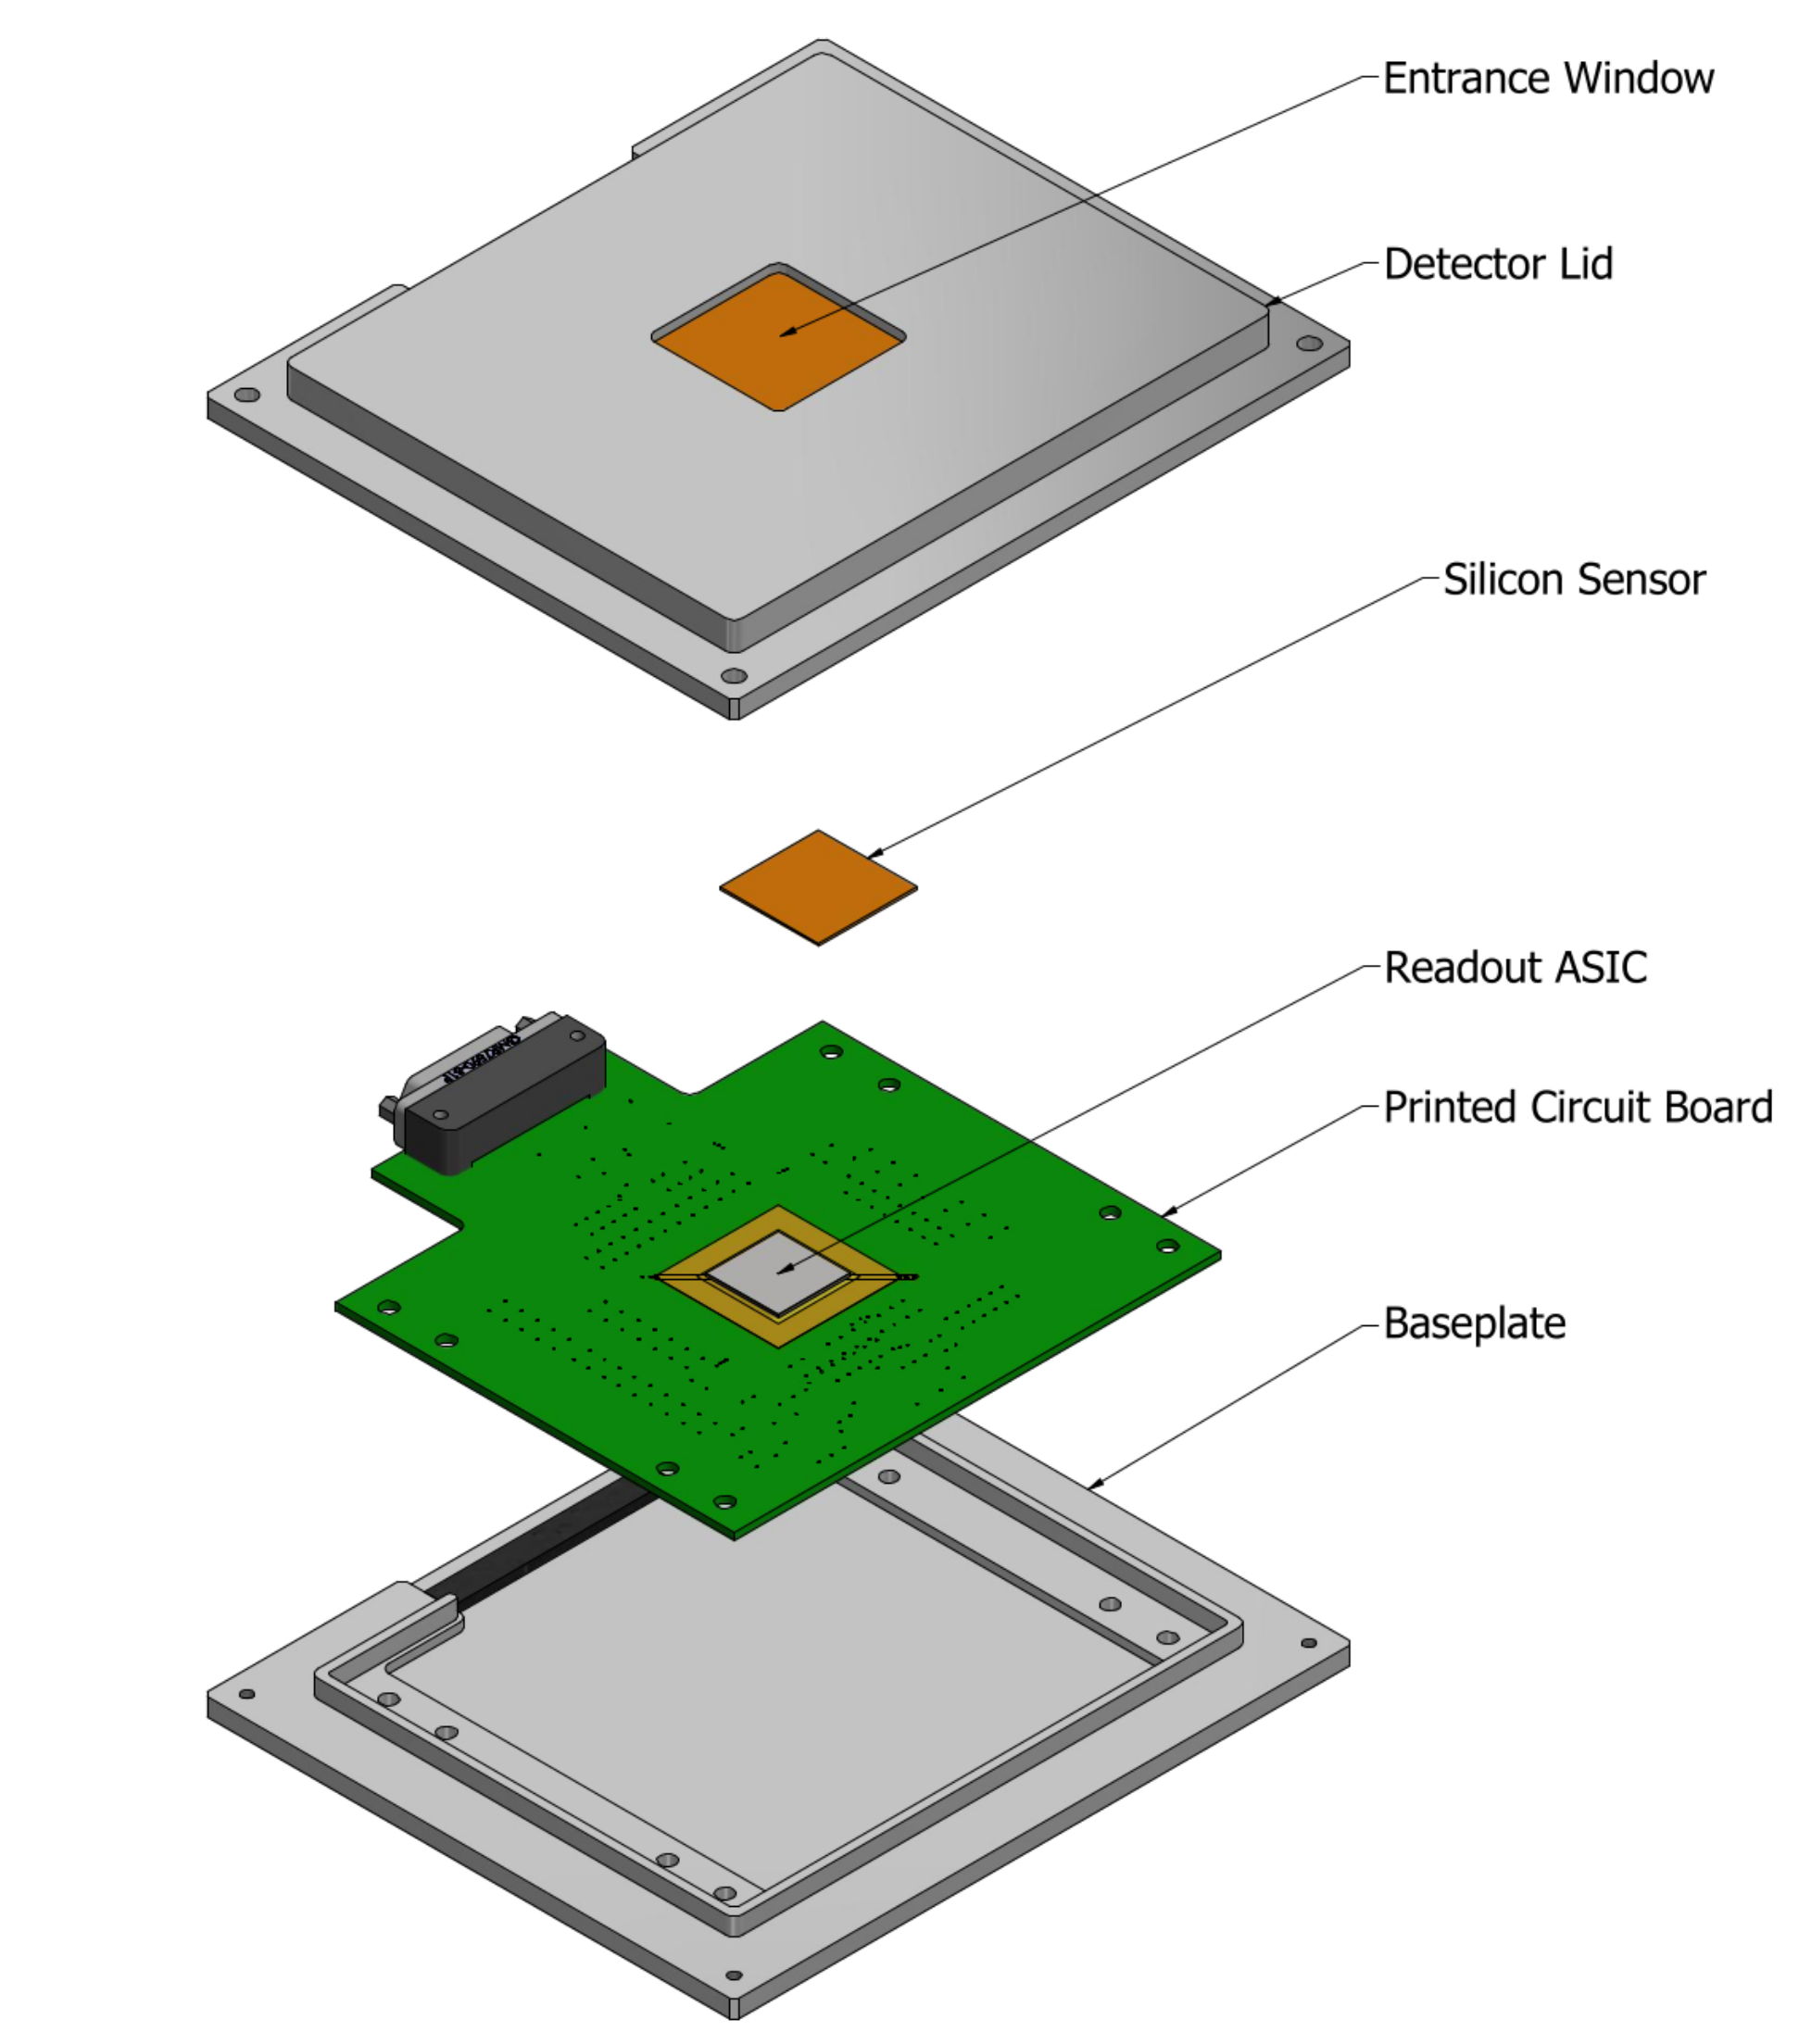
\includegraphics[width=0.7\linewidth]{figures/chapter4/design/detector}
    \caption{Exploded view of the detector with its housing. The detector is placed inside a simple metal housing with a square entrance window of a material suited for X-ray detection, such as beryllium or plastic materials. The detector itself is composed of the semiconductor sensor bump-bonded on top of the readout ASIC, which is wire bonded to the electronic board.}
    \label{fig:detector}
\end{figure}


\subsection{Active sensor}
\label{subsec:sensor}

The active sensor is the component of the detector where the physical signal is generated by interaction mechanisms between radiation and the sensor material, which is ionized by charged particles or by the photoelectron generated by the absorption of electromagnetic radiation \cite{rossi2006}. In solid state detectors the active sensor is made of a semiconductor material. 

There are various choices for the sensor material, depending on the required properties of the detector and the type or radiation that has to be detected. ASIX, which is designed to work with soft and hard X-rays, currently employs silicon and cadmium-telluride (CdTe) in the two prototypes currently available. CdTe is best suited for the harder region of the electromagnetic spectrum, as cadmium and tellurium are high-$Z$ materials, thus they have a cross section higher than silicon and a higher photoabsorption efficiency, as shown in Figs. \ref{fig:photo_cross_section} and \ref{fig:photoabs}.

The two active sensor prototypes consist of an hexagonally pixelated n-on-p 300 $\mu$m thick silicon sensor with a pixel pitch of 50 $\mu$m and an hexagonally pixelated Schottky-type 750 $\mu$m thick CdTe sensor with a pixel pitch of 100 $\mu$m \cite{minuti2025}, shown in Fig. \ref{fig:cdte_proto}. Given that the currently available ASIC readout chip has hexagonal pixels with 50 $\mu$m pitch, the CdTe sensor requires to connect one out of every four readout pixels.

\begin{figure}
    \centering
    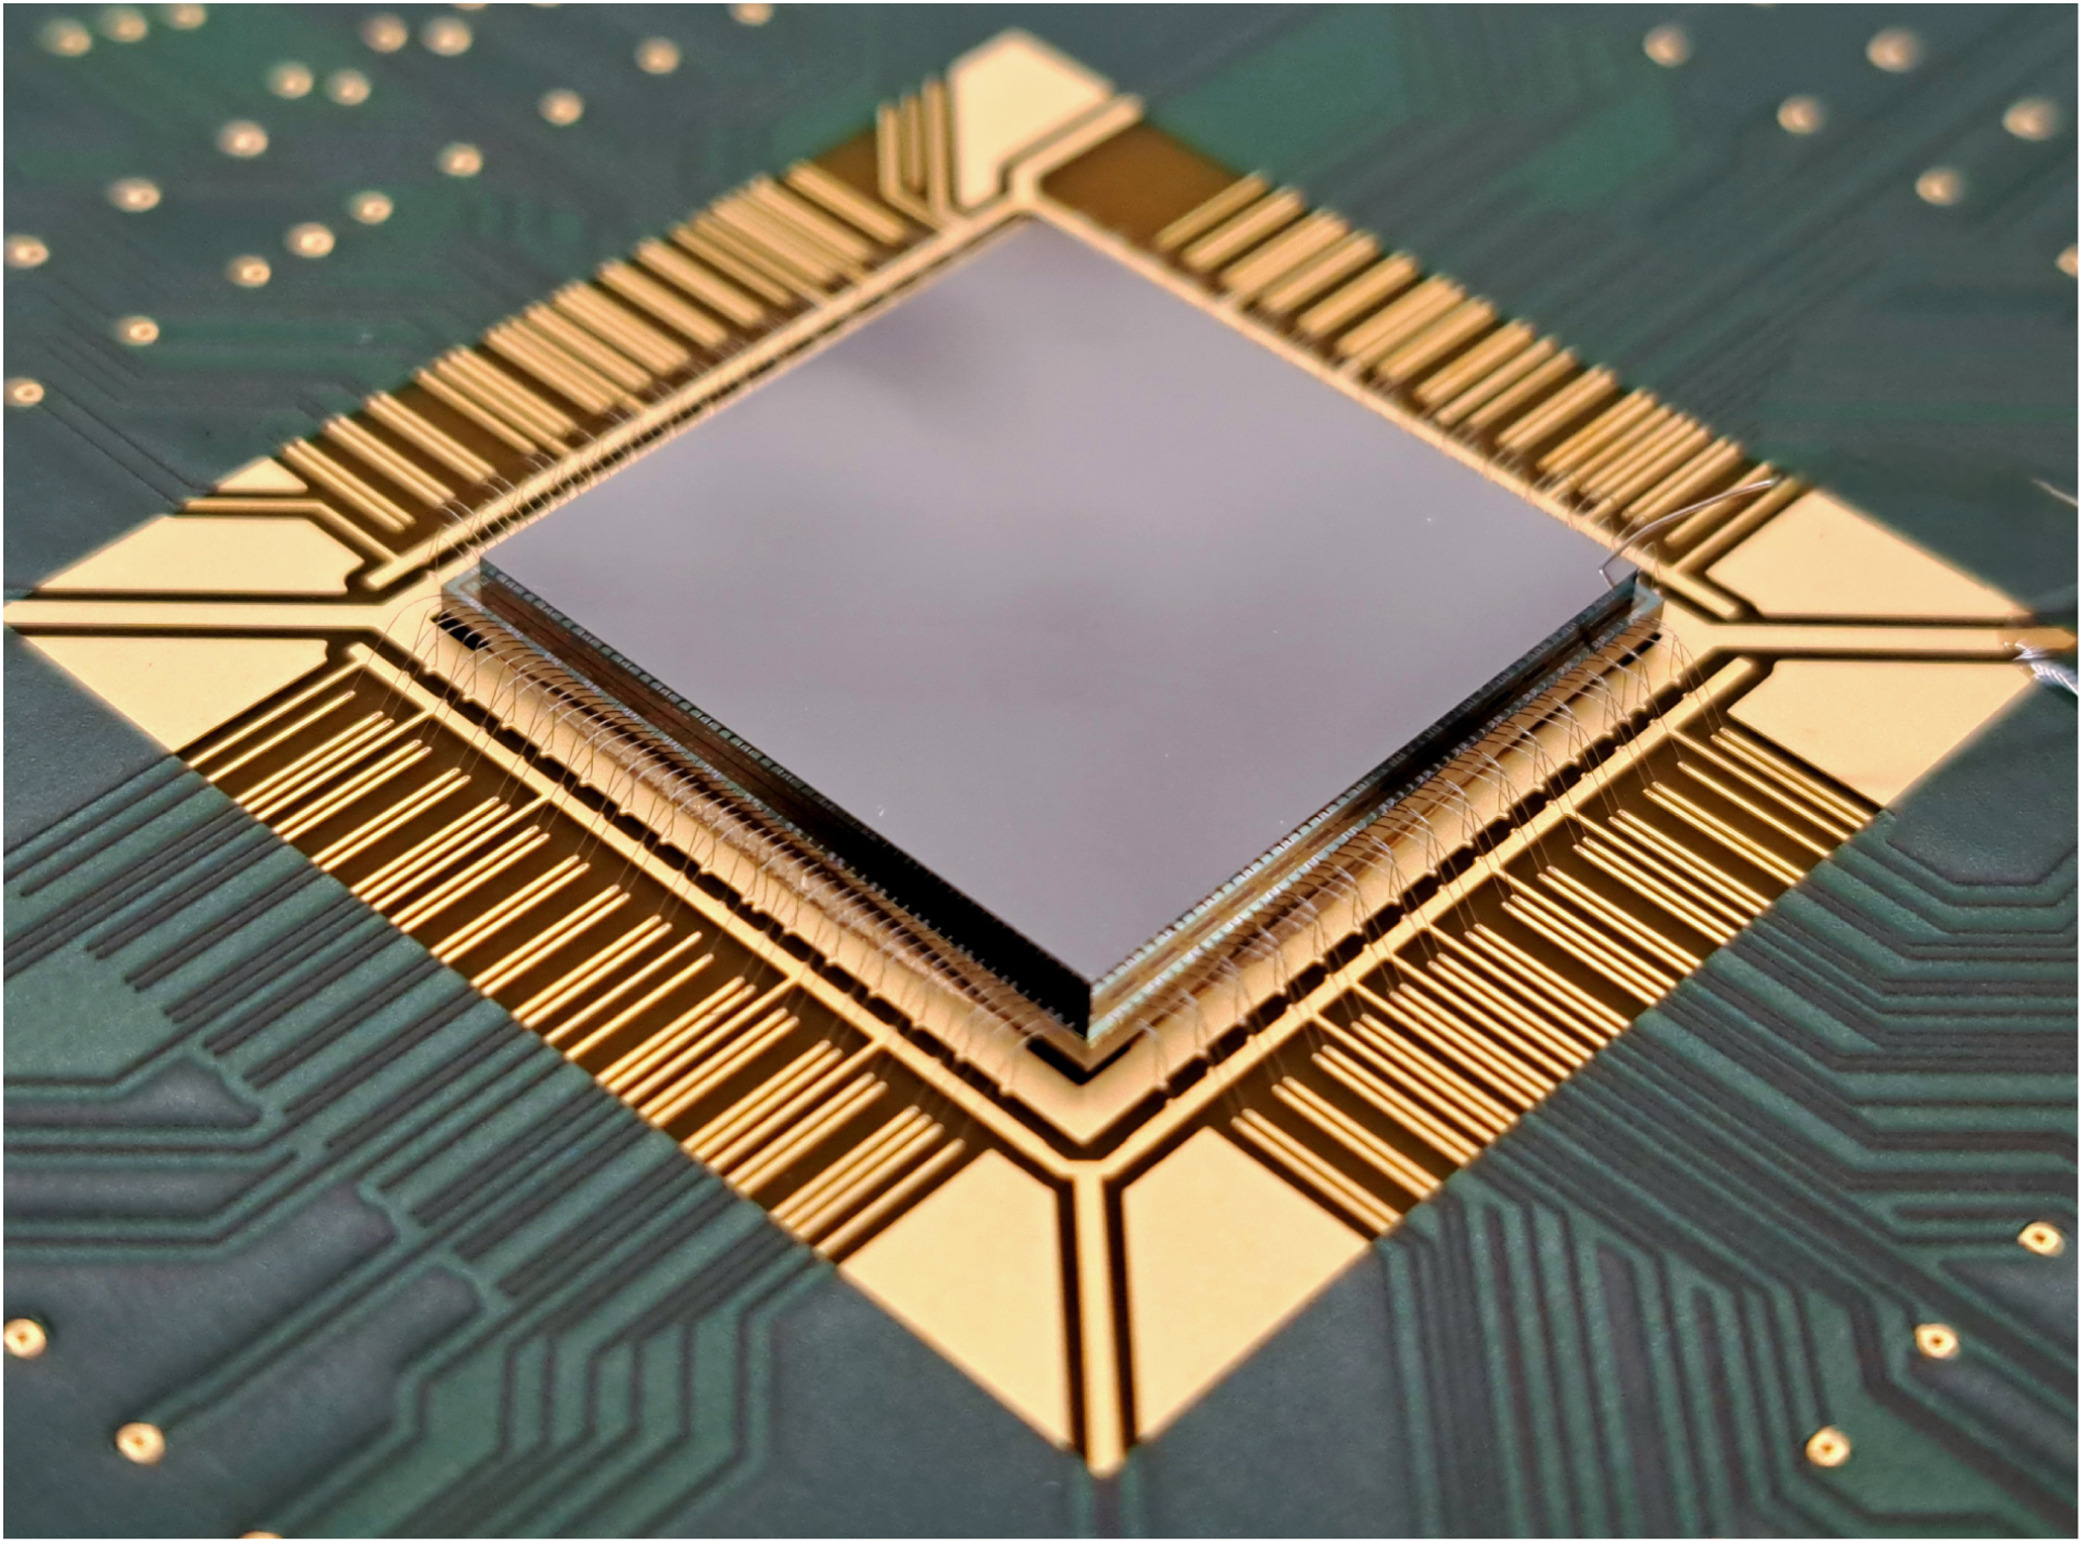
\includegraphics[width=0.7\linewidth]{figures/chapter4/design/asix}
    \caption{ASIX hybrid pixel detector with the CdTe sensor. The metallic layer visible on top is a platinum electrode positioned on the back side of the CdTe sensor to apply the reverse bias voltage. Image taken from \cite{minuti2025}.}
    \label{fig:cdte_proto}
\end{figure}

When a photon is absorbed in the active sensor, the distance traveled by the photoelectron depends on its kinetic energy and the sensor material, but it is typically much smaller than the sensor thickness (e.g., in silicon for $E_{\gamma} < 10~\text{keV}$, the photoelectron range is less than $1~\mu\text{m}$ \cite{nist_estar}). Consequently, the region where electron-hole pairs are generated via ionization can be approximated as point-like and coincident with the photon absorption point.

Once electron-hole pairs are generated they start to diffuse in the plane perpendicular to the electric field, as described in Chap. \ref{sec:semiconductors}. Knowing the sensor material properties, the electric field and the working conditions of the detector (e.g. the sensor temperature), the transverse diffusion sigma can be calculated using Eq. \ref{eq:diff_sigma_dist}.

The absorption depth depends on the energy of the photon and is distributed according to Eq. \ref{eq:pdf_truncated}, and by fixing the sensor thickness it allows to calculate the mean transverse diffusion sigma $\langle \sigma \rangle$ from Eqs. \ref{eq:z_average} and \ref{eq:diff_sigma_dist}. The dependence of $\langle \sigma \rangle$ on the photon energy for different Si sensor thicknesses is shown in Fig. \ref{fig:mean_sigma}.

\begin{figure}
    \centering
    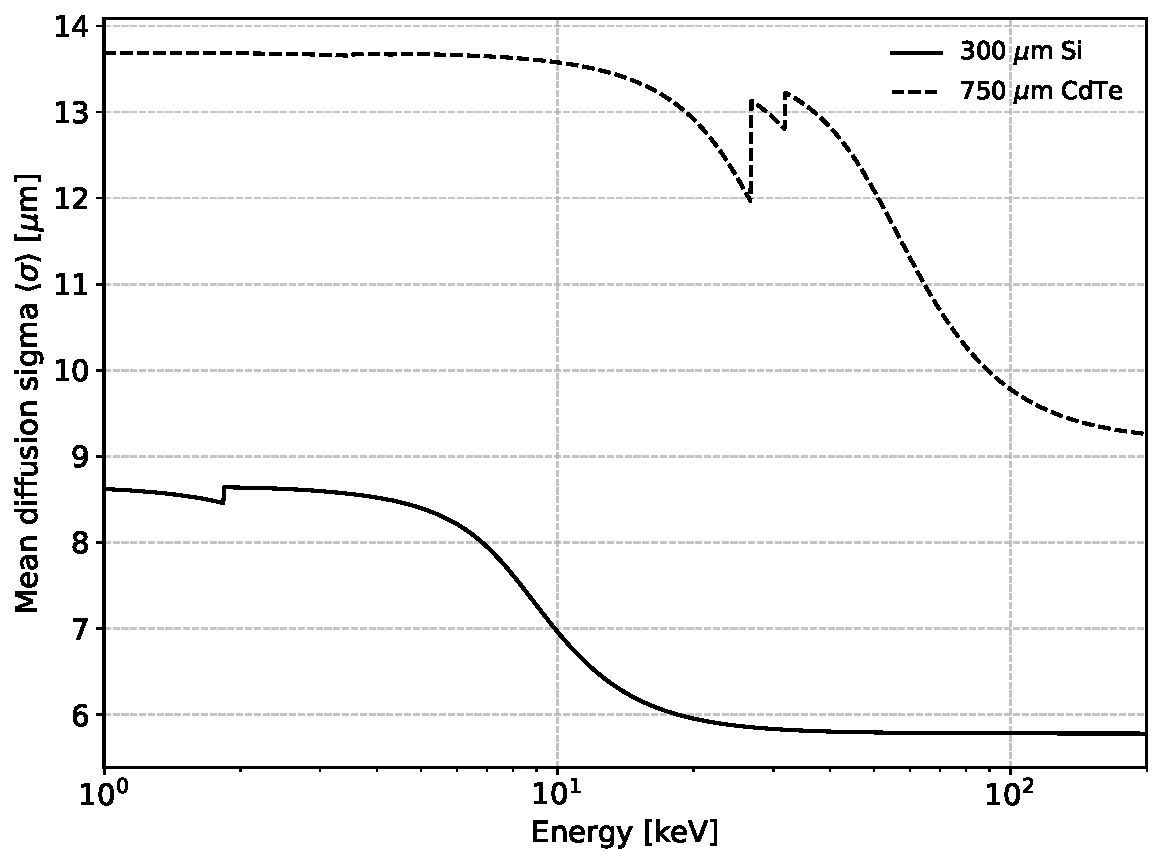
\includegraphics[width=0.7\linewidth]{figures/chapter4/design/mean_diffusion}
    \caption{Mean diffusion sigma as a function of the photon energy for different thickness of Si sensors, assuming $\mathcal{D} = 50 \,\mu$m cm$^{-0.5}$. }
    \label{fig:mean_sigma}
\end{figure}

Once the sensor working conditions like the temperature and the electric field are determined, meaning that $\mathcal{D}$ is fixed, Eq. \ref{eq:z_average} allows to find the best values of the sensor thickness and pixel pitch depending on the main intent of the detector.

If the goal is an imaging detector, the best choice would be to produce a large charge diffusion cloud in order to hit a lot of pixels and then reconstruct the position even with simple algorithms. Conversely, for spectroscopy applications, the smaller the number of pixels involved in the event, the better the energy resolution, as the total readout noise on the final measurement scales as $\sqrt{N}$, where $N$ is the number of pixels involved.

ASIX's goal is to find a compromise between an imaging and a spectroscopy detector, and thanks to a low noise readout and the pixel size and geometry, a good performance for both tasks is achievable. For this reason the sensor thickness and pixel pitch are chosen in order to have a ratio between the charge diffusion sigma and the pixel pitch $\langle \sigma \rangle / p$ in the range between 10--20\%.

The relevant metric to gauge how this ratio affects the detector readout design and the event analysis is the cluster size, which is defined as the number of pixels that have a signal above a certain threshold.

Simulations of charge diffusion show that in this range of $\langle \sigma \rangle / p$ the cluster size is always smaller than eight. This means that, given the hexagonal geometry of the pixels, all the charge is contained inside a circular set of seven pixels, with the pixel with the most charge at the center of the set and the other six pixels arranged in a circular corona around it. As will be discussed in Chap. \ref{subsec:readout}, this feature defines the readout logic of the chip under development.

Another important property which depends on diffusion and detector geometry is how the charge is distributed across the pixels. This is essential to determine the imaging and spectroscopy performance of the detector. As shown in Fig. \ref{fig:charge_distr}, by analyzing simulated events uniformly distributed across the pixels, the pixel charge distribution is highly asymmetrical and on average more than 90-95\% of the charge is always collected by two pixels and the third pixel collects almost all of the remaining charge, while the other four pixels always have less than 1\% of the total charge.

In real working conditions, even with low-noise readout electronics, is highly probable that the charge collected by each one of these four pixels is comparable to the electronic noise or even smaller. 

\begin{figure}
    \centering
    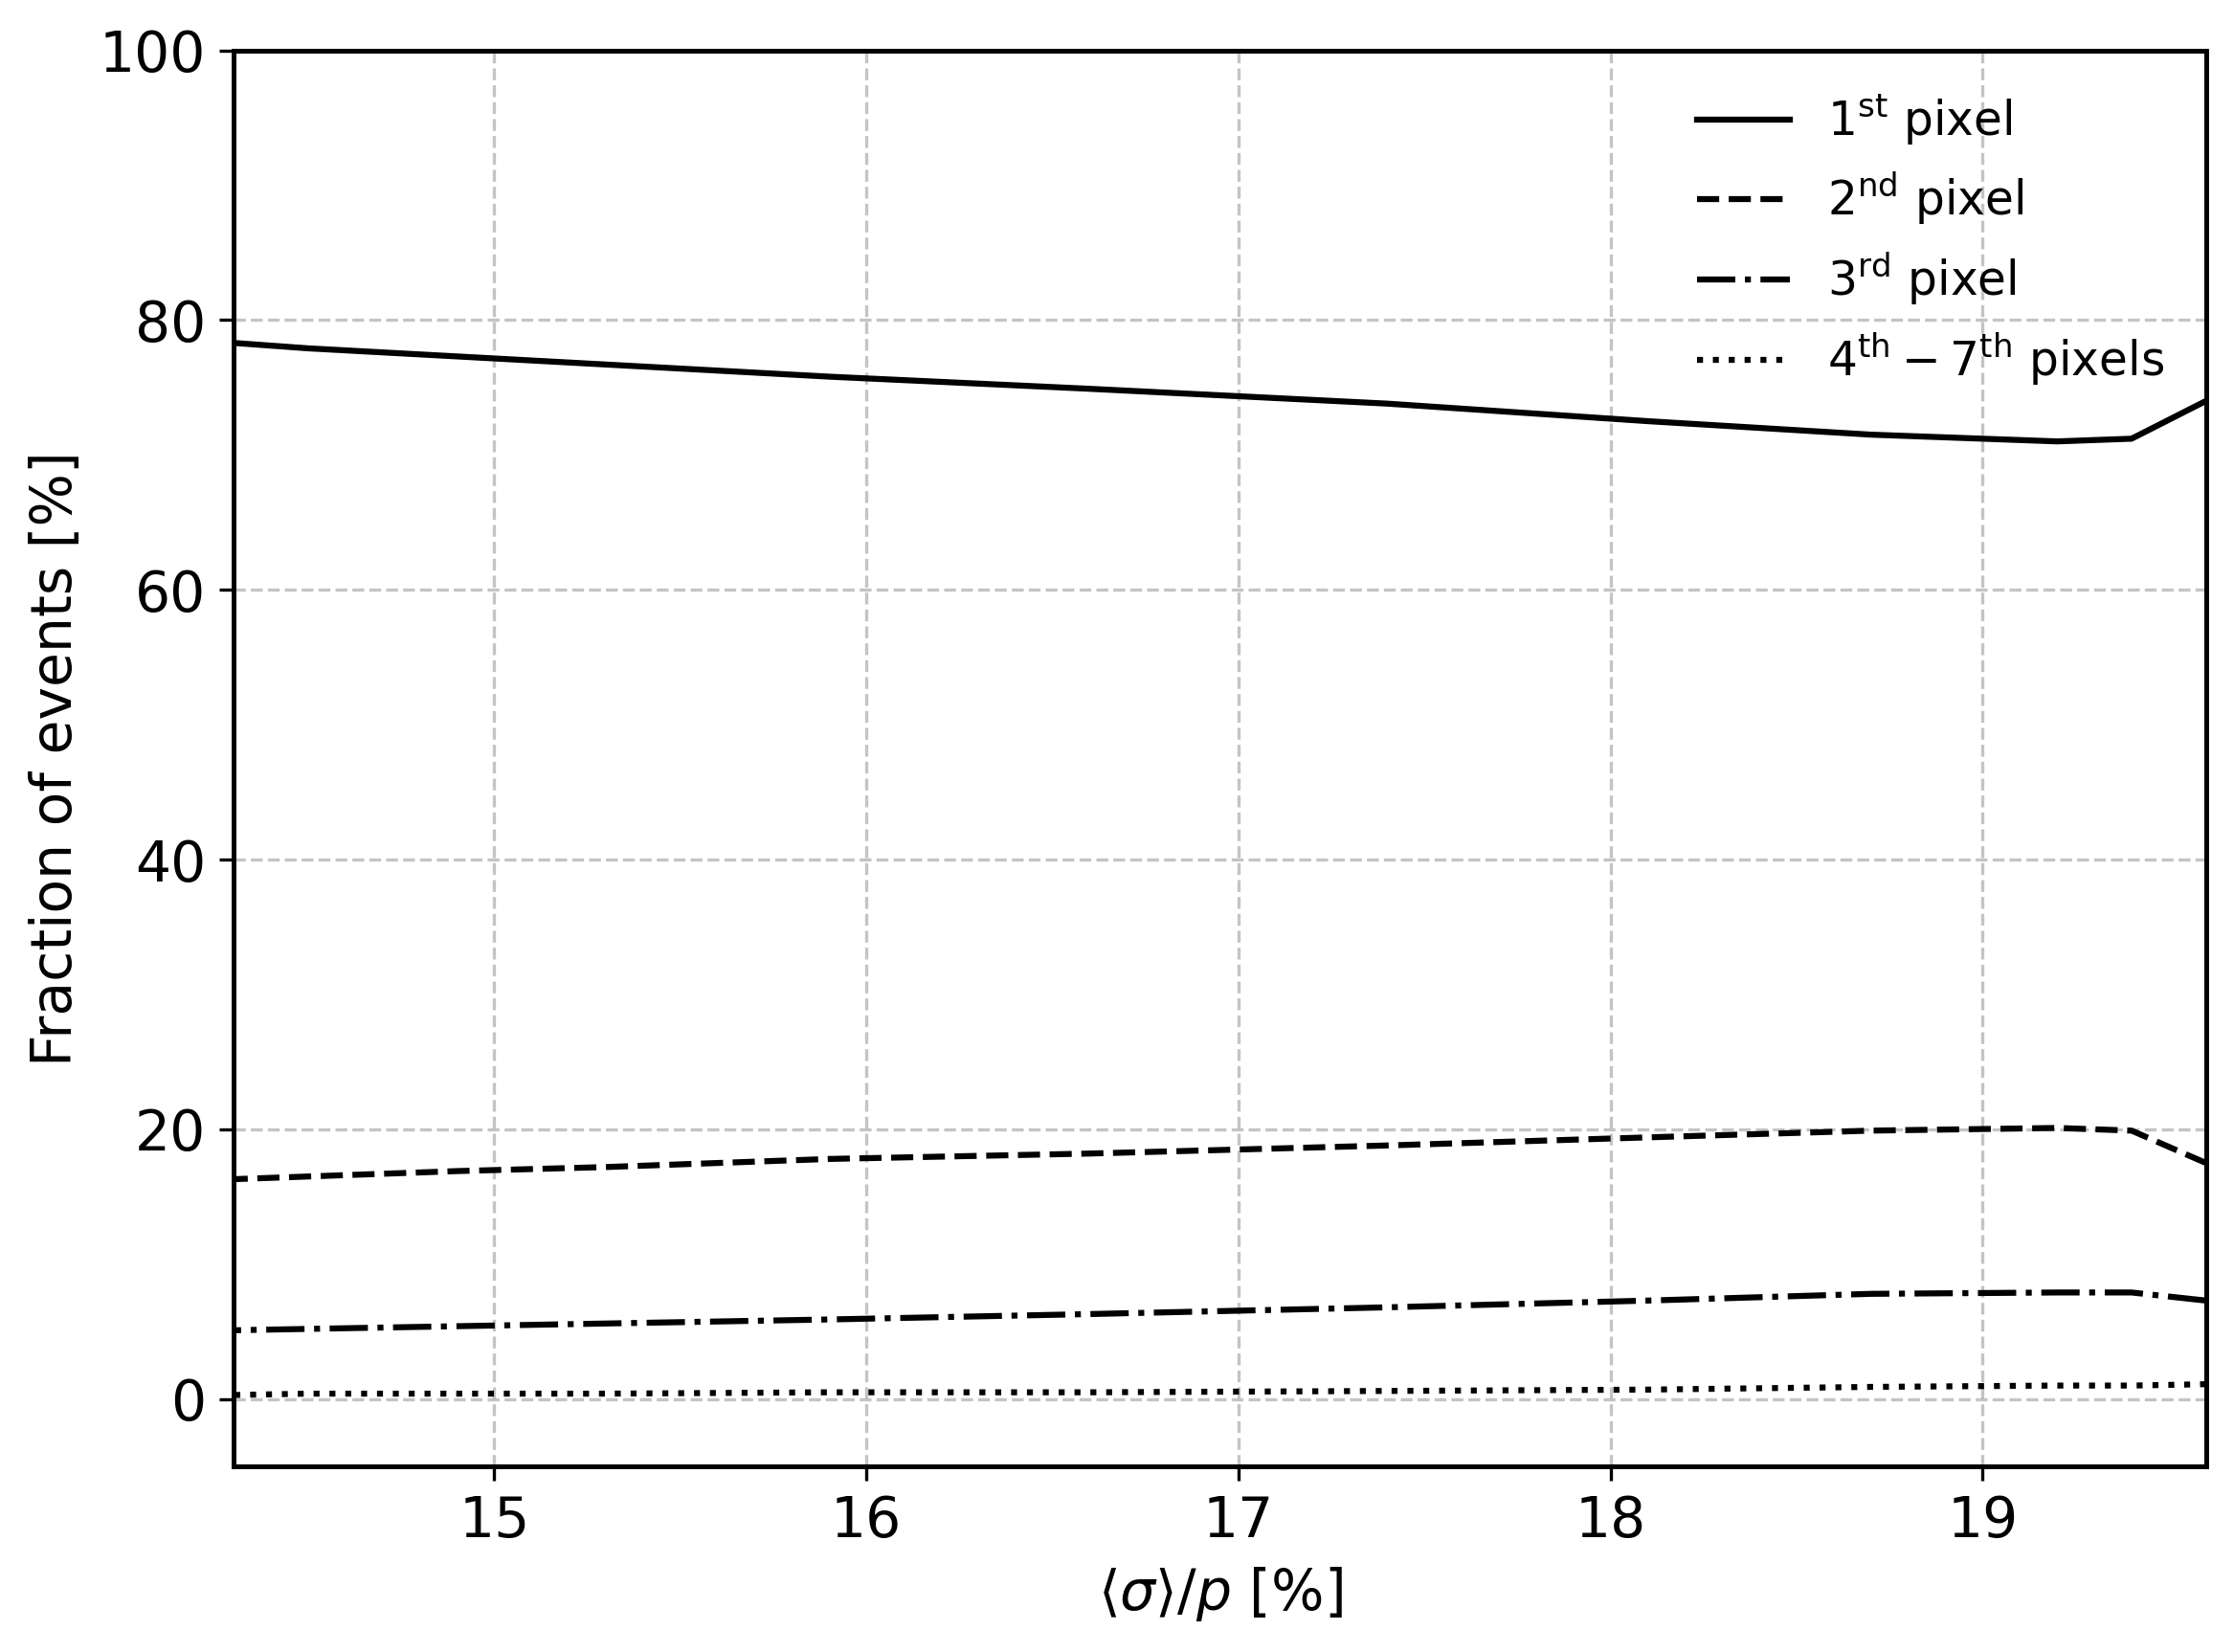
\includegraphics[width=0.7\linewidth]{figures/chapter4/design/charge_distr}
    \caption{Average charge fraction collected by the first, second, third and the remaining pixels as a function of $\langle \sigma \rangle / p$. The data set used consists of a simulation with uniformly distributed events across the pixels without electronic noise and no clustering threshold has been used.}
    \label{fig:charge_distr}
\end{figure}

%\begin{table}[htbp]
%\centering
%\begin{tabular}{c cccc}
%\multirow{2}{*}{$\langle \sigma \rangle / p$ [\%]} & \multicolumn{4}{c}{Pixel charge [\%]} \\
%\cmidrule(lr){2-5}
% & 1 & 2 & 3 & 4--7 \\
%\midrule
%19.6 & 74.0 & 17.5 & 7.3 & 1.1 \\
%19.4 & 71.2 & 19.9 & 7.9 & 1.0 \\
%19.2 & 71.0 & 20.1 & 7.9 & 1.0 \\
%18.7 & 71.5 & 19.9 & 7.8 & 0.9 \\
%18.1 & 72.5 & 19.4 & 7.3 & 0.7 \\
%17.4 & 73.8 & 18.8 & 6.8 & 0.6 \\
%16.6 & 74.9 & 18.2 & 6.3 & 0.5 \\
%15.9 & 75.8 & 17.8 & 5.9 & 0.5 \\
%15.3 & 76.7 & 17.2 & 5.6 & 0.4 \\
%14.9 & 77.3 & 16.9 & 5.4 & 0.4 \\
%14.5 & 77.9 & 16.5 & 5.2 & 0.4 \\
%14.3 & 78.3 & 16.3 & 5.1 & 0.3 \\
%\bottomrule
%\end{tabular}
%\caption{Average charge fraction collected by cluster pixels for different values of the ratio between the mean transverse diffusion sigma and the pixel pitch. The simulated data set is the same as Tab. \ref{tab:cluster_size}. It can be observed that the majority of the charge is collected by the first three pixels. \fix{Sostituire con grafico in cui su asse x c'è s/p, su y mettiamo occorrenza, plottiamo 1 pixel, 2 pixel, 3 pixel, sum(4-7) pixel, magari anche sum(1-2)}}
%\label{tab:charge_distr}
%\end{table}

\subsection{Readout strategy}
\label{subsec:readout}

The major difference between a GPD and the detectors developed under the ASIX project lies in the track topology. In a GPD, a photoelectron track can be up to a millimeter long (tens of pixels) due to the low density of the gaseous active medium, and its morphology varies significantly with photon energy. In a solid-state detector, instead, the charge is confined within a few tens of micrometers (a few pixels, typically no more than three, and strictly fewer than eight), as shown in Fig. \ref{fig:charge_distr}.

Furthermore, the charge distribution is axially symmetric around the impact point. As previously mentioned, this topology results in an event that is fully contained within a region composed of a central pixel (which collects most of the charge) and its six immediate neighbors.

Given this fixed maximum dimension and geometry, the readout can be performed differently from that of a GPD. The core idea is that when a pixel exceeds the trigger threshold, it is read out together with all six surrounding neighbors, regardless of the charge they have collected; therefore, the readout process always involves a fixed geometry seven-pixel cluster.

This represents a remarkable difference with respect to GPDs, requiring a completely new chip designed to fully exploit the advantages offered by this compact event topology. An example of the readout strategy is shown in Fig. \ref{fig:adc_routing}.

\begin{figure}[htbp]
    \centering
    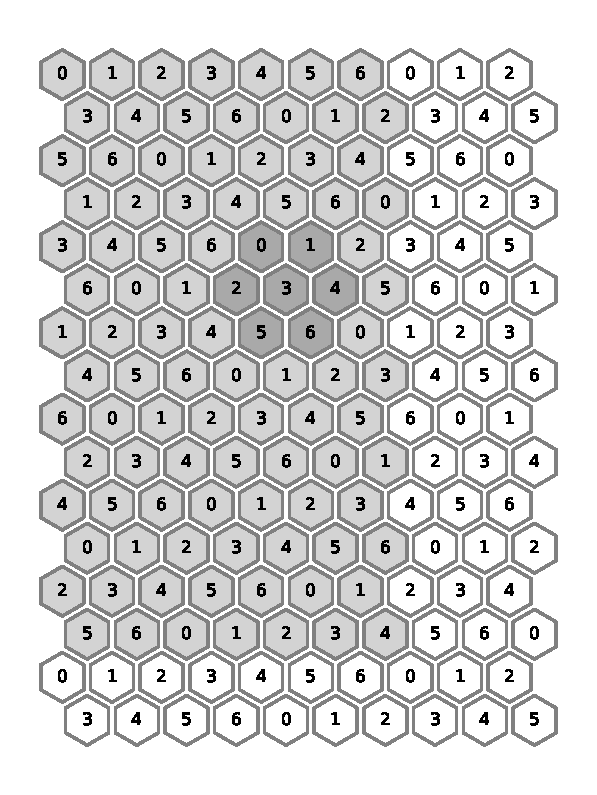
\includegraphics[width=0.4\linewidth]{figures/chapter4/design/adc_routing}
    \caption{Example of pixel routing using seven independent ADC channels. Each pixel is labeled with its corresponding ADC channel. The light gray area highlights the minimal unit cell needed to avoid adjacent pixels sharing the same channel. The seven darker pixels illustrate a cluster read out after the pixel connected to channel 3 triggers the event.}
    \label{fig:adc_routing}
\end{figure}


\subsection{ASIC}
\label{subsec:asic}

The goal of developing a detector suitable for different applications under diverse operating conditions requires a readout chip capable of handling event rates significantly higher than those typical of astrophysical sources. As a reference, the brightest extrasolar source in the 2--8~keV energy range yields a flux of about 30~ph~cm$^{-2}$~s$^{-1}$, whereas an XRD laboratory setup with a Cu source can easily exceed a flux of $2 \times 10^8$~ph~cm$^{-2}$~s$^{-1}$ \cite{bolze2019}.

The key to speeding up the readout with respect to GPDs is exploiting the fixed event geometry. While reducing the number of pixels to read is essential to lower the dead time, the main architectural breakthrough is the ability to read all seven pixels in parallel. 

This parallel readout can be implemented using an external ADC with seven independent channels. Each pixel in a cluster is routed to a different channel, and the hexagonal honeycomb arrangement of the pixels is ideal for this purpose, as it allows the entire chip matrix to be mapped using seven channels without any adjacent repetition of the same channel. This configuration enables a 7-pixel cluster to be read out in parallel at any location on the chip, as illustrated in Fig. \ref{fig:adc_routing}.

A further increase in rate capability can be achieved by segmenting the chip into independent readout regions, each equipped with its own 7-channel ADC. Although this approach can truncate events occurring at the boundaries between regions, leading to their rejection, selecting an optimal region size and shape ensures that the fraction of rejected events remains negligible.

The current design goal is to achieve a maximum rate capability of at least 100~kHz per region at a readout clock frequency of 20~MHz, which translates into a global detector rate of about 1~MHz, depending on the final number of independent regions.

The minimal event structure for readout requires to save the coordinates of the highest pixel (9 + 9 bit for a $304 \times 352$ pixels chip), the content of the pixels ($12 \times 7$ bit, assuming to use a 12 bit ADC) and the timestamp (16 bit), with a total event size of 118 bit. With a global rate of 1 MHz it would require a data bus with the capability of transferring around 100 MBit/s, which is feasible.

This performance estimate assumes that pedestal subtraction is performed offline, unlike in previous XPOL chips. Indeed, since all seven pixels are sampled simultaneously by their dedicated ADC channels, systematic effects induced by time-dependent digital transients during serial readout are naturally avoided. This eliminates the need for a second pedestal readout pass, saving time at the cost of requiring an accurate offline pedestal calibration.

Another critical property, essential for high-resolution spectroscopy, is the Equivalent Noise Charge (ENC) introduced by the front-end electronics. The design target is to maintain the noise below 20~$e^-$ ENC per pixel. When coupled with a silicon sensor, this noise level yields an energy resolution of approximately 350~eV FWHM at 8~keV, which is sufficient to resolve the Cu-K$_{\alpha}$ (8.04 keV) and Cu-K$_{\beta}$ (8.90 keV) fluorescence lines commonly used in XRD setups.

All these requirements are achievable with a dedicated analog front-end ASIC. The proposed design features $50~\mu\text{m}$ pitch hexagonal pixels in a honeycomb array over a rectangular matrix, similar to the other XPOL family chips. However, unlike in GPDs, where the readout pixels are physically separated from the GEM, in the ASIX architecture the ASIC pixels are directly connected to the pixelated sensor via micro-bump soldering, aligning each ASIC pixel to the corresponding electrode on the sensor.

Finally, to preserve the chip versatility for applications such as X-ray polarimetry, it will be designed to support an alternative triggering and readout logic similar to XPOL-III, based on a sequential readout within a rectangular ROI, as described in Chap. \ref{sec:xpol3}. While this mode operates at lower speeds and reduced maximum rates, it allows the acquisition and reconstruction of extended photoelectron tracks when required.

At the moment, the dedicated ASIC is still in the design phase and prototypes are not yet available.

\section{Simulations and analysis framework}

To estimate the properties of different detector designs prior to the realization and then to characterize a prototype, a framework to generate Monte Carlo simulations of the detector and analyze collected data has been developed and is available at \cite{hexsample, tomaiuolo2024}. The framework provides a suite of command-line tools that can be executed directly from the terminal or integrated into automated scripts. Data are stored using the Hierarchical Data Format (HDF5), which allows for efficient array storage and metadata tagging through file attributes. The core pipeline modules, illustrated in Fig.~\ref{fig:block_diagram}, are responsible for running Monte Carlo simulations, converting raw binary data collected with prototypes into HDF5 files, performing detector calibration, and executing event reconstruction.

This section illustrates the Monte Carlo simulation software and the calibration and analysis pipeline.

\begin{figure}[h]
    \centering
    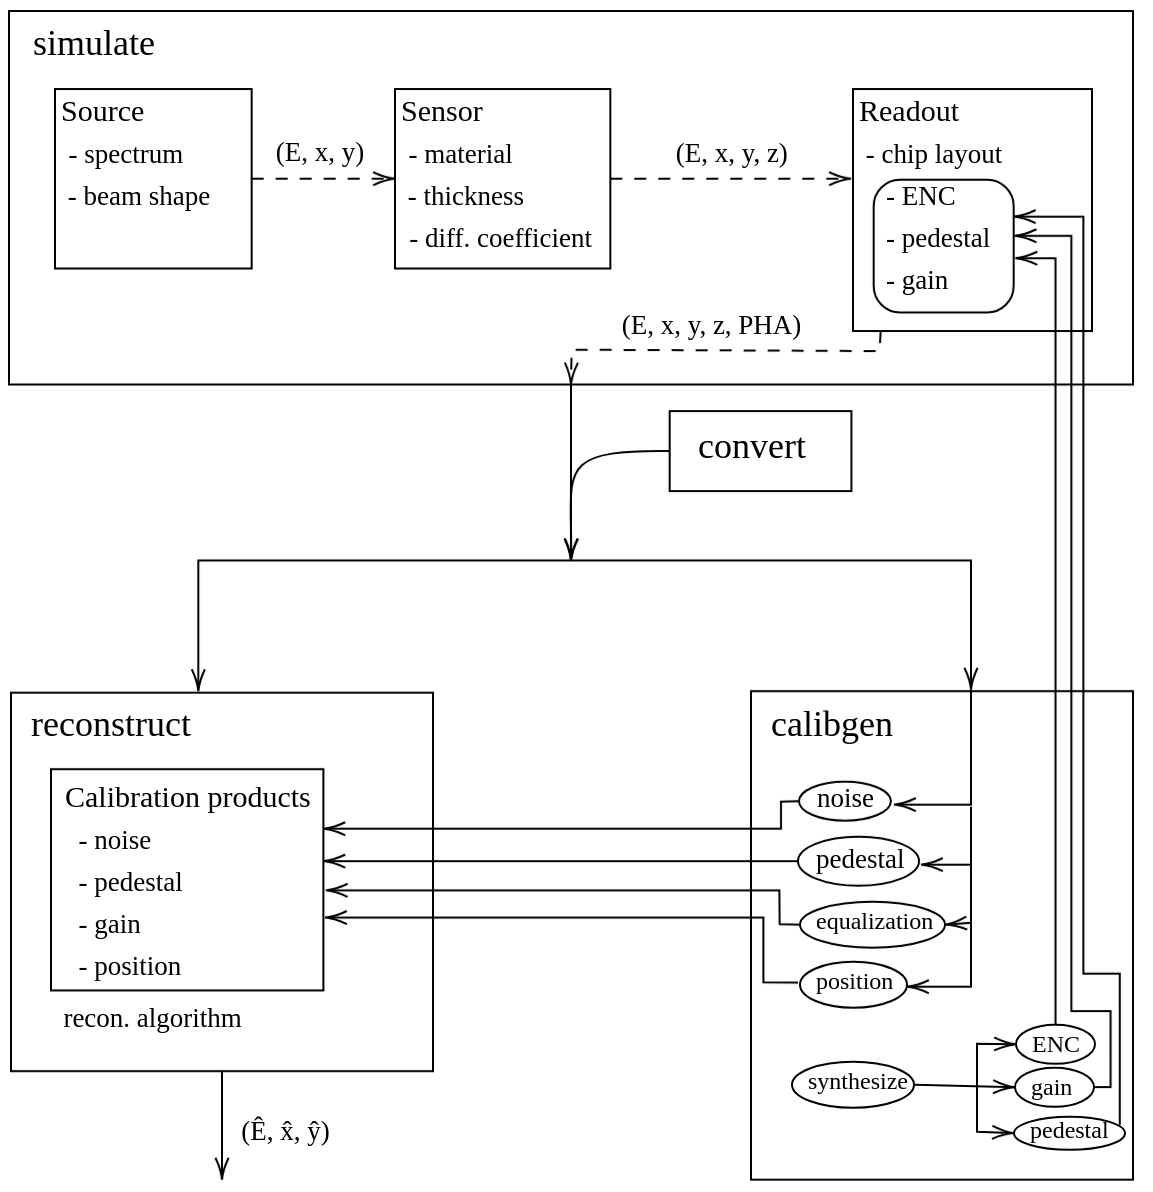
\includegraphics[width=0.7\linewidth]{figures/chapter4/calibration/block_diagram}
    \caption{Block diagram representing the main steps of the simulation and analysis software available at \cite{hexsample}. A dataset can be generated with the Monte Carlo simulation framework or obtained by converting a binary laboratory acquisition. The dataset is used to generate the calibration products, which are subsequently employed to reconstruct the events.}
    \label{fig:block_diagram}
\end{figure}

\subsection{Monte Carlo simulations}
Monte Carlo simulations of the detector are essential to understand its capabilities depending on the design. As mentioned in the previous section, designing a detector which has both imaging and spectroscopical high-resolution capabilities requires to carefully tune the active sensor thickness, pixel pitch, working voltages and further properties to achieve the correct trade-off between energy and spatial resolution. 

With the first prototypes it is also possible to validate the simulations with laboratory data, and if necessary finely tuning the Monte Carlo to match the data, in order to have a software that can reliably simulate the real detector. The simulation consists of different steps, each representing a different stage of the detector.

First, it is necessary to define the detector design, specifying the active sensor and the readout chip properties. The active sensor is described by three parameters, which are the material, the thickness and the transverse diffusion coefficient of the electrons, defined in Eq. \ref{eq:diff_sigma_dist} and that depends on the working conditions.

The chip layout is described by the pixel pitch, the number of columns and rows and the readout logic, which allows to choose between the seven-pixels parallel readout and the XPOL-III sequential rectangular readout with the additional option to choose the padding dimensions. The readout chip is also characterized by three other quantities, the ENC, the pedestal and the gain, which are provided in form of matrices with the same dimension of the chip to take into account spatial variations across the chip. The last thing to setup is the X-ray source, which is described by its energy spectrum and the beam shape, position and spatial distribution.

In the simulation, a photon with a given energy and incident position is generated according to the spectrum and beam distribution and then its absorption depth is sampled from Eq. \ref{eq:pdf_truncated}.

At the moment, only on-axis photons generation is implemented. Furthermore, the approximation that electron-hole pairs are produced in a point-like region located in the absorption point is adopted. As mentioned above, this approximation is valid in the case of a silicon sensor and photon energies below 10 keV.

The diffusion is modeled as discussed in Chap. \ref{subsec:sensor}, assuming a two-dimensional Gaussian distribution centered on the impact point and with a standard deviation which depends on the absorption depth. Afterwards, the event readout is performed according to the chosen readout logic.

The simulation does not take into account some physical effects, such as the distance travelled by the photoelectron or the possibility of having a fluorescence photon that can travel through the sensor before being absorbed, with the consequence that a point-like conversion region is no more a good approximation.

As mentioned above, the first effect becomes relevant at high photon energies, while the second effect depends on the photon energy and the sensor material, as fluorescence yield depends on the involved shell and on the atomic number $Z$. For silicon the fluorescence yield is smaller than 5\% for K-shell and almost 0\% for L-shell, while for cadmium and tellurium is between 83-88\% for K-shell and about 5-7\% for L-shell, as shown in Fig. \ref{fig:fluorescence_yield}.

If fluorescence radiation is emitted, given the isotropic emission angle distribution, it travels through the sensor until it is absorbed and produces a new photo-electron. Depending on the photon energy, the new photoelectron can be generated even a pixel pitch far from the first electron. For CdTe sensor this drastically decreases the simulation accuracy, but only for energies above the K-edge, which is about 27 keV.

At the moment the goal of the simulation software is to validate and verify the feasibility of the silicon sensor design in the 6--10 keV energy range, thus all of these effects are negligible. In the future more detailed simulations will be performed by implementing this stage with Geant4 \cite{geant4}.

Another effect that is not taken into account is pixel crosstalk, which represents an additional source of charge sharing between pixels. A simple way to partially solve this is to include this effect into the charge diffusion process, increasing the diffusion parameter calculated from Eq. \ref{eq:diff_sigma_dist}. The correct value of this parameter can be chosen comparing the cluster size distribution between laboratory data and simulation until they match.

\subsection{Analysis}
\label{sec:analysis}
After detector calibration, which requires more details and will be explained in the next section, data files generated with Monte Carlo simulations or by converting laboratory binary data files can be analyzed to extract the relevant information about the events.

Each event contains information about the timestamp, the signal amplitude recorded by each pixel (expressed as Pulse Height Amplitude, or PHA), and the coordinates needed to localize the event, which depend on the readout mode. If using the seven-pixel parallel readout mode the coordinate of the central pixel is given, while in the XPOL-III readout mode the coordinates of two opposite vertices of the rectangular ROI and the padding information are stored.

Detector calibration is necessary because raw PHA values need to be corrected for two contributions, which are pedestal and normalized gain variations over the chip. Further details will be given in the following.

The corrected PHA values are used to analyze the event and reconstruct photon properties, such as energy and impact position. The reconstruction software contains different algorithms to infer the position and energy, and according to the one adopted an additional processing of the data can be required.

For some algorithms all the PHA values of the seven-pixel cluster are necessary, while for others a data reduction can be made. Particularly, as shown in Fig. \ref{fig:charge_distr}, more than 99\% of all the charge is collected by the three pixels with most signal. This information can be used to create a smaller cluster containing only pixels that have a high probability of having collected physical signal and not only electronic noise.

The first step to create the cluster is choosing a zero-suppression threshold, which is defined for each pixel in terms of its noise standard deviation, measured during the calibration phase to build a dedicated noise map of the chip. The threshold is used to suppress all the pixels that are dominated by electronic noise.

The second step applies a geometrical constraint, requiring all pixels above threshold to be adjacent. The central pixel is always kept as it triggered the event. The remaining pixels in the cluster are selected by evaluating the non-central pixels above threshold in descending order of signal amplitude, starting from the one with the highest PHA. A pixel is kept only if it is adjacent to a previously accepted pixel, otherwise it is suppressed. This process continues until a maximum of two neighboring pixels (plus the central one) is reached. Consequently, the final cluster size is strictly constrained to be between one and three.

\section{Detector calibration}
\label{sec:calibration}

Raw PHA values recorded by the detector need to be corrected for electronic baseline offsets (pedestal) and pixel-to-pixel gain variations (equalization) to retrieve the true deposited charge. Furthermore, characterizing the pixel noise is essential to define zero-suppression thresholds and to correctly weight PHA values during clustering and event reconstruction.

Detector calibration is crucial to account for spatial non-uniformities across the active area, which arise from small imperfections in the readout electronics, sensor inhomogeneities, and non-uniformities in the bump-bonding connections with the ASIC. Correcting for these variations allows maximizing detector performance and improving both spatial and energy resolution.

The calibration process consists in measuring the pedestal level (in ADC counts), the noise standard deviation (in ADC counts), and the normalized gain for each pixel across the matrix. The resulting maps are employed during event reconstruction to subtract offsets, set noise-dependent thresholds, and equalize the pixel response. Under specific conditions, it is also possible to derive the absolute gain and the ENC noise by combining these calibration products with additional information on the incident radiation.

In the analysis framework a calibration product has been designed as an HDF5 file containing three different matrices with the same shape as the readout chip. Each element of a matrix is associated with the pixel in the corresponding position. The labels of the three matrices and their content are the following:
\begin{itemize}[label=-]
\item \textit{values}, contains the central value of the calibrated quantity for each pixel;
\item \textit{entries}, contains the number of events used for the calibration for each pixel;
\item \textit{errors}, contains the estimated uncertainty associated with the value of the calibrated quantity for each pixel.
\end{itemize}

The calibration products can either be generated by analyzing a data file or by synthesizing maps with the chosen size and values distribution. As said above, their main use is for event reconstruction, but they are also used to define the readout chip characteristics in the Monte Carlo simulation software.

When analyzing a data file, the calibration process follows a specific order. First, noise and pedestal levels are calibrated, and then the normalized gain is evaluated using these baseline products. If required, the absolute gain and ENC maps can subsequently be calculated using the ADC noise and normalized gain maps.

In this section the methods developed to calibrate noise, pedestal and gain are described, and finally the results obtained from the calibration of Monte Carlo simulations are presented to evaluate the performance of the calibration framework.

\subsection{Noise and pedestal}
\label{sec:noise_calibration}

Noise and pedestal variations are introduced by small non-uniformities in the manufacturing of the readout electronics and in the bonding of the active sensor onto the ASIC. Characterizing the noise of each pixel enables to apply pixel thresholds that take into account the possibility of having noisier pixels. 

The noise and pedestal level are estimated by sampling the PHA distribution of a pixel in the absence of source signal. Under this condition, the PHA distribution of each pixel is a Gaussian distribution with a mean corresponding to the pedestal and a standard deviation equal to the noise of the pixel. During the readout the Gaussian is truncated before 0 ADC and digitized. In the optimal configuration, to estimate both quantities, the pedestal is much larger than the noise and thus the Gaussian can be fully sampled. 

For the current prototypes, which are based on XPOL-III, it is possible to generate noise and pedestal maps from data acquisitions with a source that illuminates the chip.  As explained in Chap. \ref{sec:xpol3}, XPOL-III defines a ROT with triggered miniclusters and an additional padding can be added, with a large enough padding it is possible to have a lot pixels without source signal.

In the acquisitions used in the following the padding is large and the resulting ROI has a size of at least $10\times13$ pixels, as shown in Fig. \ref{fig:noise_pedestal_roi}. The true size depends on the number of miniclusters that triggered, thus it can be larger. Once the ROI is defined, pixels that belong to the ROT and all their neighbors are discarded in order to have the smallest probability of including pixels with source signal in the analysis. The number of pixels resulting from this selection is about 120, but it depends on the size of the ROT.

\begin{figure}
    \centering
    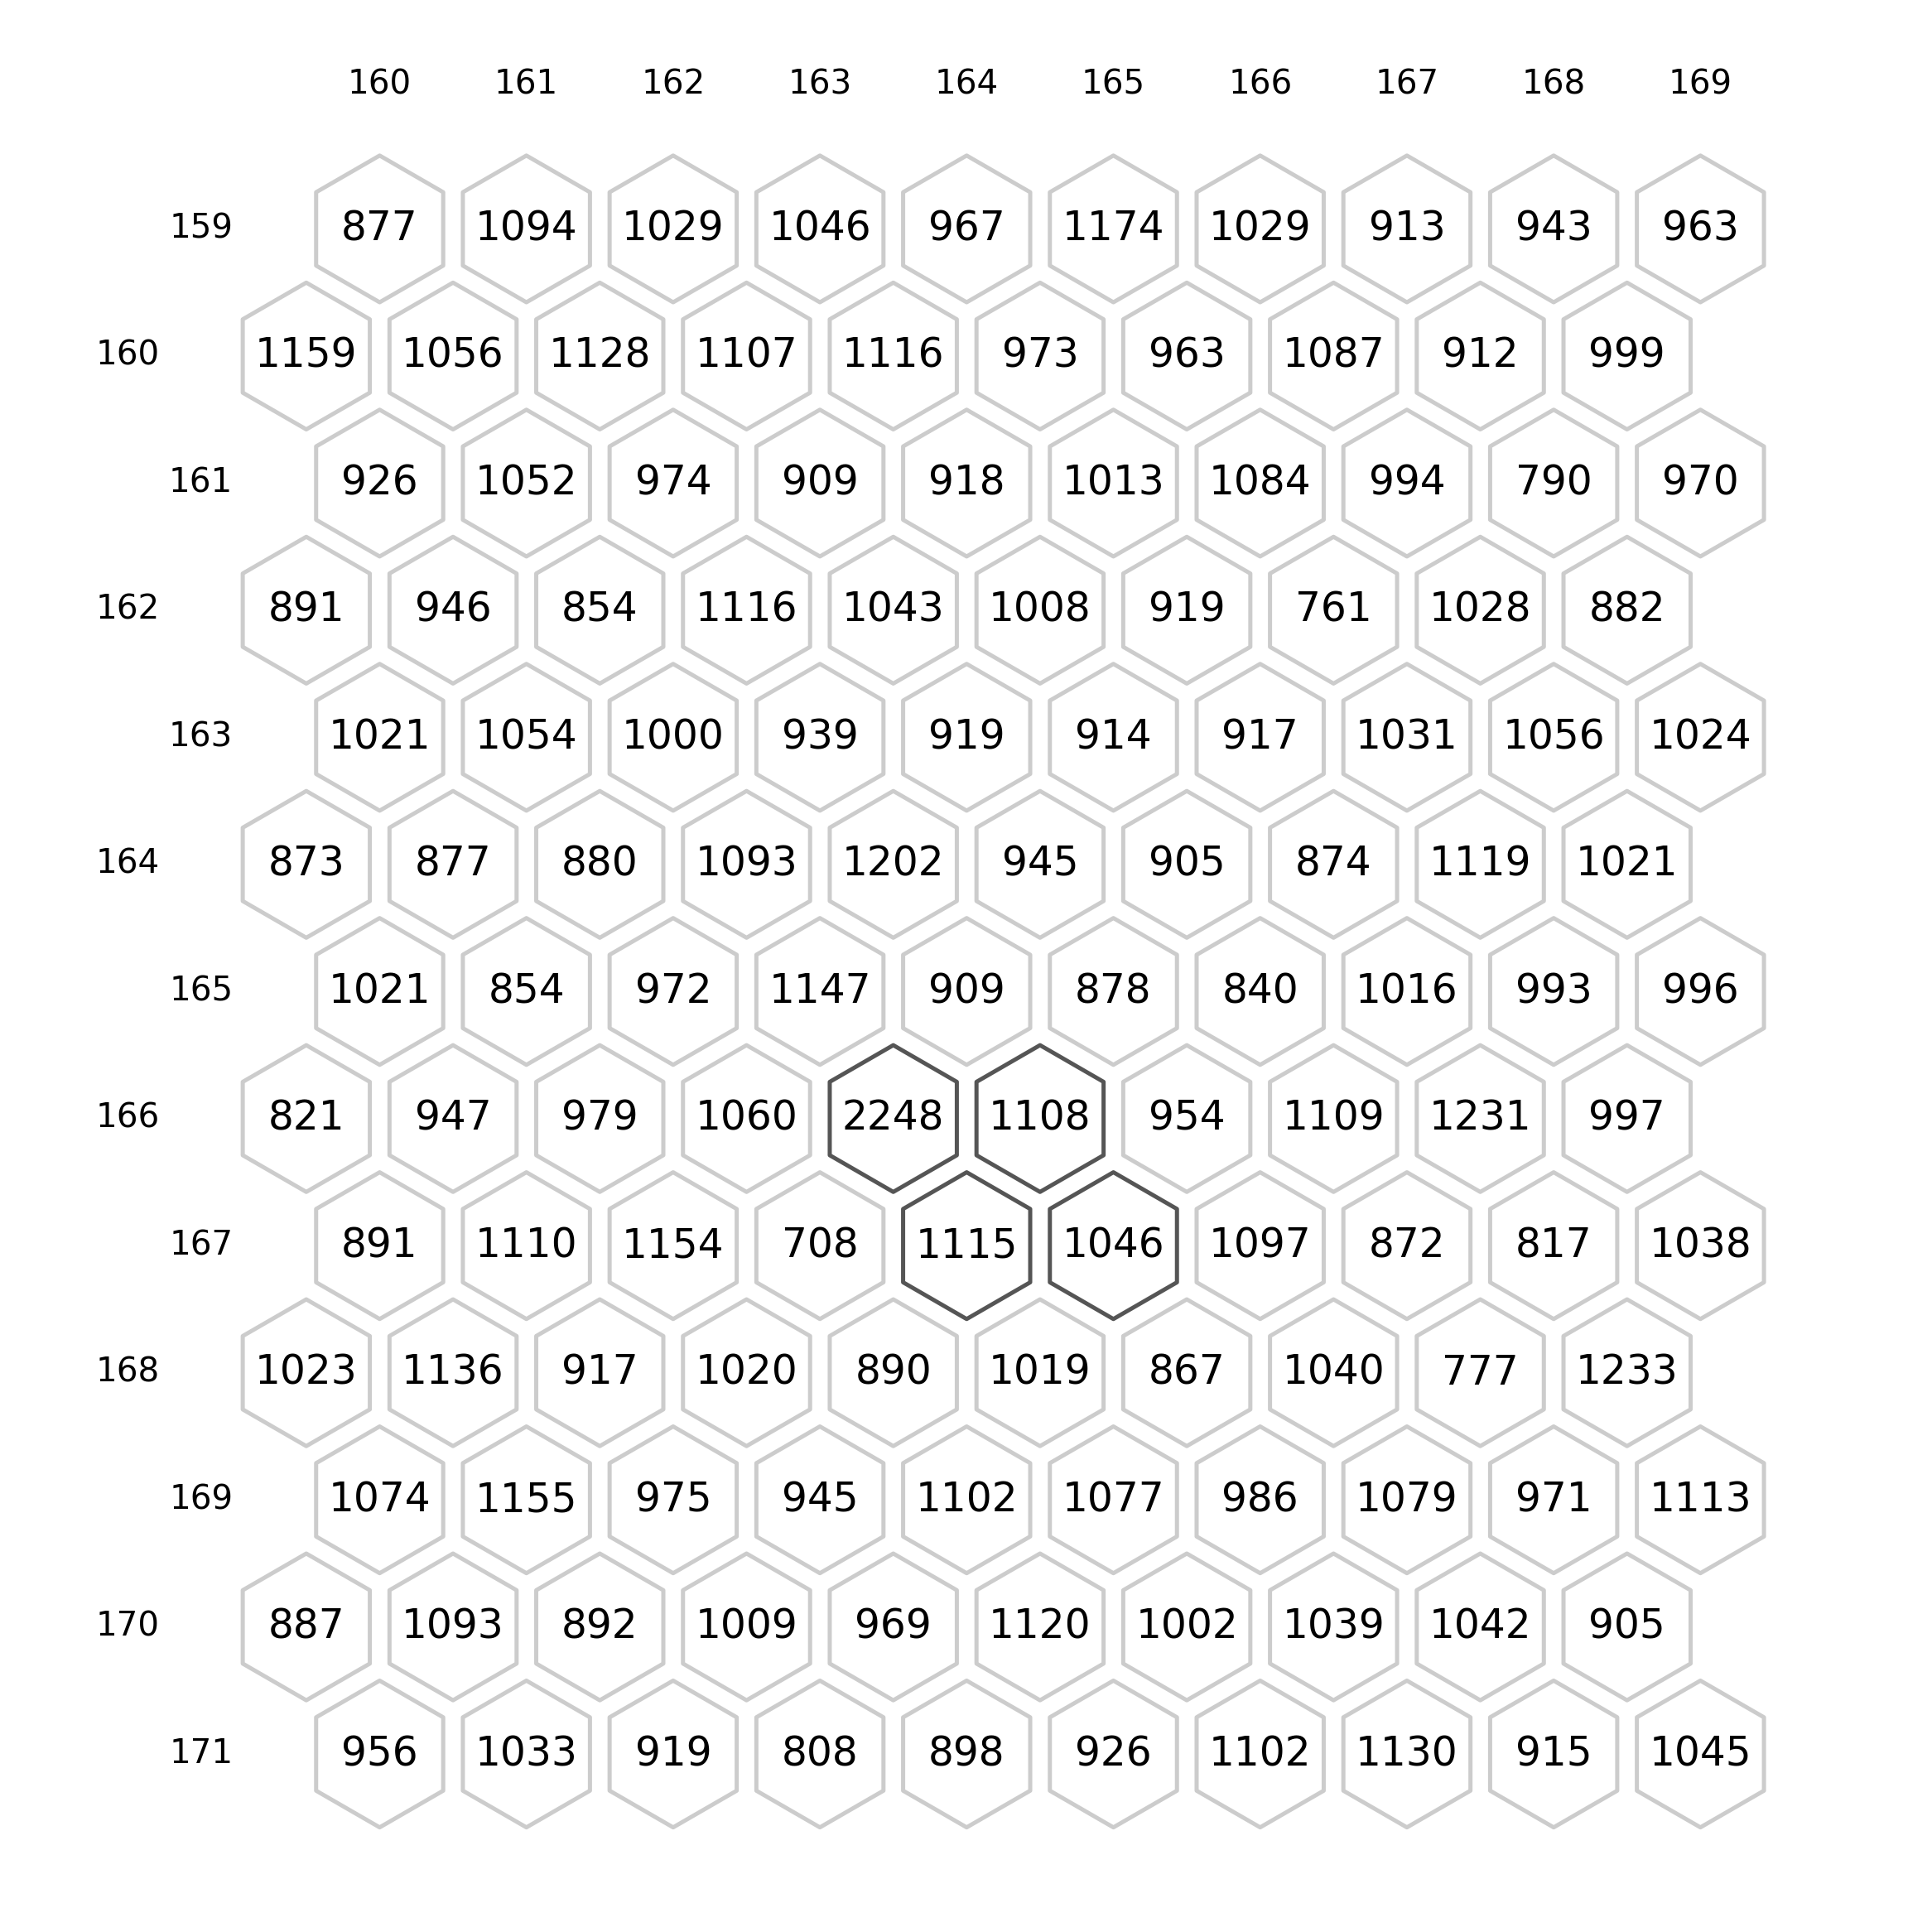
\includegraphics[width=0.5\linewidth]{figures/chapter4/calibration/roi}
    \caption{Example of the ROI of an event with the source on. Central pixels with marked borders belongs to the ROT and are excluded from the calibration analysis, together with all their immediate neighbors. This image is taken from a simulation with pixel noise and pedestals distributed according to Gaussian distributions with 20 ADC and 1000 ADC, respectively, and 10\% standard deviation.}
    \label{fig:noise_pedestal_roi}
\end{figure}

Depending on the readout properties, there are different methods that can be employed to calibrate noise and pedestals. However, in the current XPOL-III design pedestal subtraction is performed online, thus it is not possible to calibrate pedestal levels from data acquisitions. For this reason, it is assumed that they are exactly zero for all the pixels, thus only noise requires to be calibrated.

The first calibration method is used exactly in the current working condition where pedestals are zero. In this case the PHA sample distribution is a half-normal distribution defined only on the positive semi-axis, and the probability density function is

\begin{equation}
p(x; \sigma^2) = \frac{2}{\sqrt{2 \pi \sigma^2}} \exp \left( -\frac{x^2}{2\sigma^2} \right), \quad \text{for } x > 0
\label{eq:half_normal}
\end{equation}

Using the parity of the Gaussian it can be shown that the expectation value $\langle x^2 \rangle$ of the distribution defined in Eq. \ref{eq:half_normal} is equal to the variance of the untruncated Gaussian, which is exactly the square of the noise value to calibrate. The best-fit value of the pixel noise is thus given by

\begin{equation}
s = \sqrt{\frac{1}{N} \sum_i^{N} x_i^2}.
\end{equation}

The uncertainty related to this estimate is the uncertainty of the sample standard deviation, thus it is $s/\sqrt{2N}$.

In case the pedestal subtraction is performed offline, there are two possible cases in which it is possible to use different methods. The first is when the pedestal level is much larger than the noise, which is the optimal case and allows to sample the entire Gaussian distribution. On the other hand, the second case is when the pedestal level is comparable to the noise (not much smaller, otherwise the first method can be employed), thus the distribution is truncated on the left tail.

In the case where the pedestals are much larger (at least 4 or 5 times larger) than the noise it is possible to directly calculate the sample mean and standard deviation of the distribution. In practice, this method is performed using Welford algorithm \cite{welford1962} for online update of the mean and variance of each pixel distribution while looping on all the events of the acquisition. The mean and variance of the distribution after $n$ events are given by

\begin{equation}
\begin{split}
\bar{x}_n &= \bar{x}_{n-1} + \frac{x_n - \bar{x}_{n-1}}{n}, \\
M_{2,n} &= M_{2, n-1} + (x_n - \bar{x}_{n-1})(x_n - \bar{x}_n), \\
s_n^2 &= \frac{M_{2,n}}{n-1}.
\end{split}
\label{eq:welford}
\end{equation}

This method ensures very high numerical stability, is fast and the occupied space in memory only depends on the shape of the detector and not on the number of processed events. The error associated to the pedestal $\hat{p}$ is the uncertainty of the sample mean, and for the noise $\hat{n}$ is the one associated to the sample standard deviation, thus

\begin{equation}
\sigma_{\hat{p}} = \frac{\hat{n}}{\sqrt{N}}, \quad \quad \sigma_{\hat{n}} = \frac{\hat{n}}{\sqrt{2N}},
\label{eq:noise_uncertainty}
\end{equation}
where $N$ is the number of events collected for each pixel.

In the last case, when the pedestals are comparable to the noise, a least-squares minimization using a Gaussian curve as the fit model can be performed for each pixel. Furthermore, this method is not stable in the limit where the PHA distribution is a half-truncated digitized Gaussian because the fit rarely converges to acceptable values.

Fig. \ref{fig:methods} shows the possible cases of application of the three methods described above. At the moment the method employed on real data is the first, but all of them can be used when the new chip, whose design phase is not completed, will be ready.

\begin{figure}[t]
    \centering
    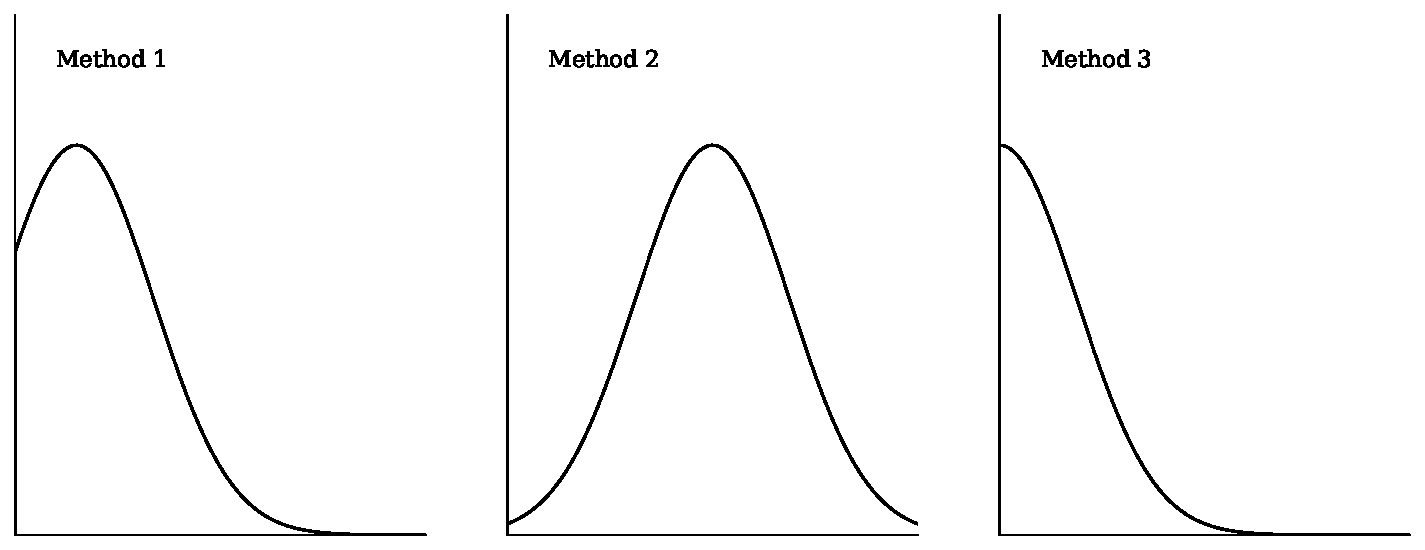
\includegraphics[width=1\linewidth]{figures/chapter4/calibration/noise_methods}
    \caption{Examples of applications of the different methods to estimate noise and pedestal levels of te detector. Method 1 can be applied when the pedestal is null and the distribution is a half-normal. Method 2 is ideal when the distribution is not truncated, thus the sample mean and standard deviation are correct. Method 3 is essential when the Gaussian is partly truncated, because the other methods do not converge to the correct values.}
    \label{fig:methods}
\end{figure}

For the first two methods the relative error on the noise calibration scales as $1/\sqrt{N}$, thus to achieve a 1\% uncertainty it is necessary to collect about $10^4$ events for each pixel. Considering that with the ROI described above about $10^2$ pixels can be used for calibration, and considering that an XPOL-III chip has more than $10^5$ pixels, the total number of events required is of the order of $10^7$. The relative error on pedestal calibration depends on the noise level.


\subsection{Normalized gain}

The accuracy of the reconstructed photon energy and incidence position is particularly sensitive to variations in pixel response across the chip. For this reason, compensating for these non-uniformities is essential to optimize the overall detector performance. These variations can be attributed to imperfections from the ASIC manufacturing process, differences in the bump-bonding connections between the ASIC and the sensor, or inhomogeneities in the sensor itself. While the former can in principle be corrected using internal ASIC calibrations, the latter require dedicated measurements with a reference source.

To calibrate this quantity it is customary to illuminate the chip with a source. In principle, there is no constraint on how the source spectrum should be, but the best results are achievable with a monochromatic source. The calibration can be performed in two different ways, depending on the knowledge of the incoming spectrum and the ability to simulate it.

The first method does not require any previous knowledge of the spectrum, as it only uses one-pixel events, which are events where all the charge is deposited in a single pixel. The idea is that when considering only one-pixel events, all the pixels have PHA distibutions with the same shape but can be shifted. Thus, by comparing the mean value of each pixel spectrum, it is possible to normalize their values by constraining the mean values distribution to have unit average.

To correctly identify one-pixel events, the clustering procedure described in Chap. \ref{sec:analysis} is applied. The zero-suppression threshold, which is determined for each pixel based on the noise calibration maps, should be set low enough to ensure that even small amounts of charge deposited into neighboring pixels due to charge diffusion are properly detected, thus preventing multi-pixel events from being misclassified as one-pixel events.

The second method is based on the modeling of the source spectrum, which is then used as a probability density function $f(E)$ to calculate the likelihood of the total charge collected by an event. Contrary to the first method, this one requires to know exactly the source spectrum and being able to simulate it for the fully calibrated and equalized detector.

To estimate $f(E)$, a dataset with the source spectrum is simulated, the event reconstruction is performed and the resulting ADC values distribution is transformed into a probability density function. This operation is performed using gaussian kernel density estimation (KDE). The resulting KDE is evaluated for a grid of values and the resulting values are then interpolated with a cubic spline. This step is necessary because KDE evaluation is slow, and given that this method relies on the numerical minimization of the negative log-likelihood, the cubic spline speeds up the minimization. KDE and interpolation are performed using functions implemented in the scientific analysis library \cite{scipy2020}.

The total energy released in an event can be expressed as the sum of the ADC counts of each pixel $p_i$ multiplied by a factor $q_i$, thus the likelihood can be calculated as

\begin{equation}
\mathcal{L}(q_1, ..., q_n) = f \left( \sum_{i=1}^n q_i p_i \right),
\label{eq:equalization_likelihood}
\end{equation}
where $n$ is the number of pixel involved in a single event. $q_i$ represents the inverse of the gain normalization, and the choice of fitting the inverse is to have more stability in the fit. Given that all events are independent, the total likelihood is the product of Eq. \ref{eq:equalization_likelihood} for each event.

This method includes all the events in the analysis, guaranteeing a much larger statistics than the other one, thus allowing to have more accuracy and stability. It is still possible to suppress pixels below a certain threshold to avoid large noise contamination.

In theory it could be possible to calculate the total likelihood for all the $N$ events across all the $n_{pix}$ pixels of the detector

\begin{equation}
\mathcal{L}(q_1, ..., q_{n_{pix}}) = \prod_{i=1}^{N} f \left( \sum_{j=1}^{n_{pix}} q_j p_j \right)
\label{eq:total_likelihood}
\end{equation}
and minimize it with respect to all the fit parameters. In practice, this is not feasible due to the large number of parameters, which are more than $10^5$, because the minimization would require too much space in memory.

For this reason the detector can be virtually divided into smaller square sub-regions and all the pixels inside the same sub-region are fitted simultaneously. In order to include an event inside a sub-region fit, all the charge must be collected by pixels inside it. To not exclude events that involve pixels on the borders of sub-regions, a two-pixel overlap is guaranteed between adjacent sub-regions. In this way all the events are considered for the analysis and pixels that lie on the borders do not have reduced statistics. For each sub-region the negative log-likelihood is calculated from Eq. \ref{eq:total_likelihood} and then minimized with \textit{iminuit} \cite{iminuit}.

If the spectrum used for the calibration is accurately simulated, it is also possible to estimate the conversion factor from ADC counts to eV, allowing the absolute gain calibration product to be obtained. Knowing the sensor material and the mean energy required to generate an electron-hole pair, it is then possible to combine the ADC noise and absolute gain maps to estimate the ENC map, thus measuring the intrinsic noise level of each pixel.

\subsection{Calibration performance}

To test the calibration procedure and gauge the algorithms performance, a dataset with a monochromatic source of 10 keV with a beam that uniformly illuminates the entire detector has been simulated. Noise, pedestal and gain are distributed according to Gaussian distributions with a mean of 100 electrons, 1000 ADC and 0.1 ADC/electron, respectively, and a standard deviation of 10\% of the mean. A total of $10^7$ events have been generated.

The first calibration step is the ADC noise and pedestal calibration. In this case the method that calculates the sample mean and standard deviation of the PHA distributions has been used because the pedestal is much bigger than the noise level. Fig. \ref{fig:noise_pedestal} shows the correlation between the calibrated and the Monte Carlo truth values of noise and pedestals.

\begin{figure}[!b]
    \centering
    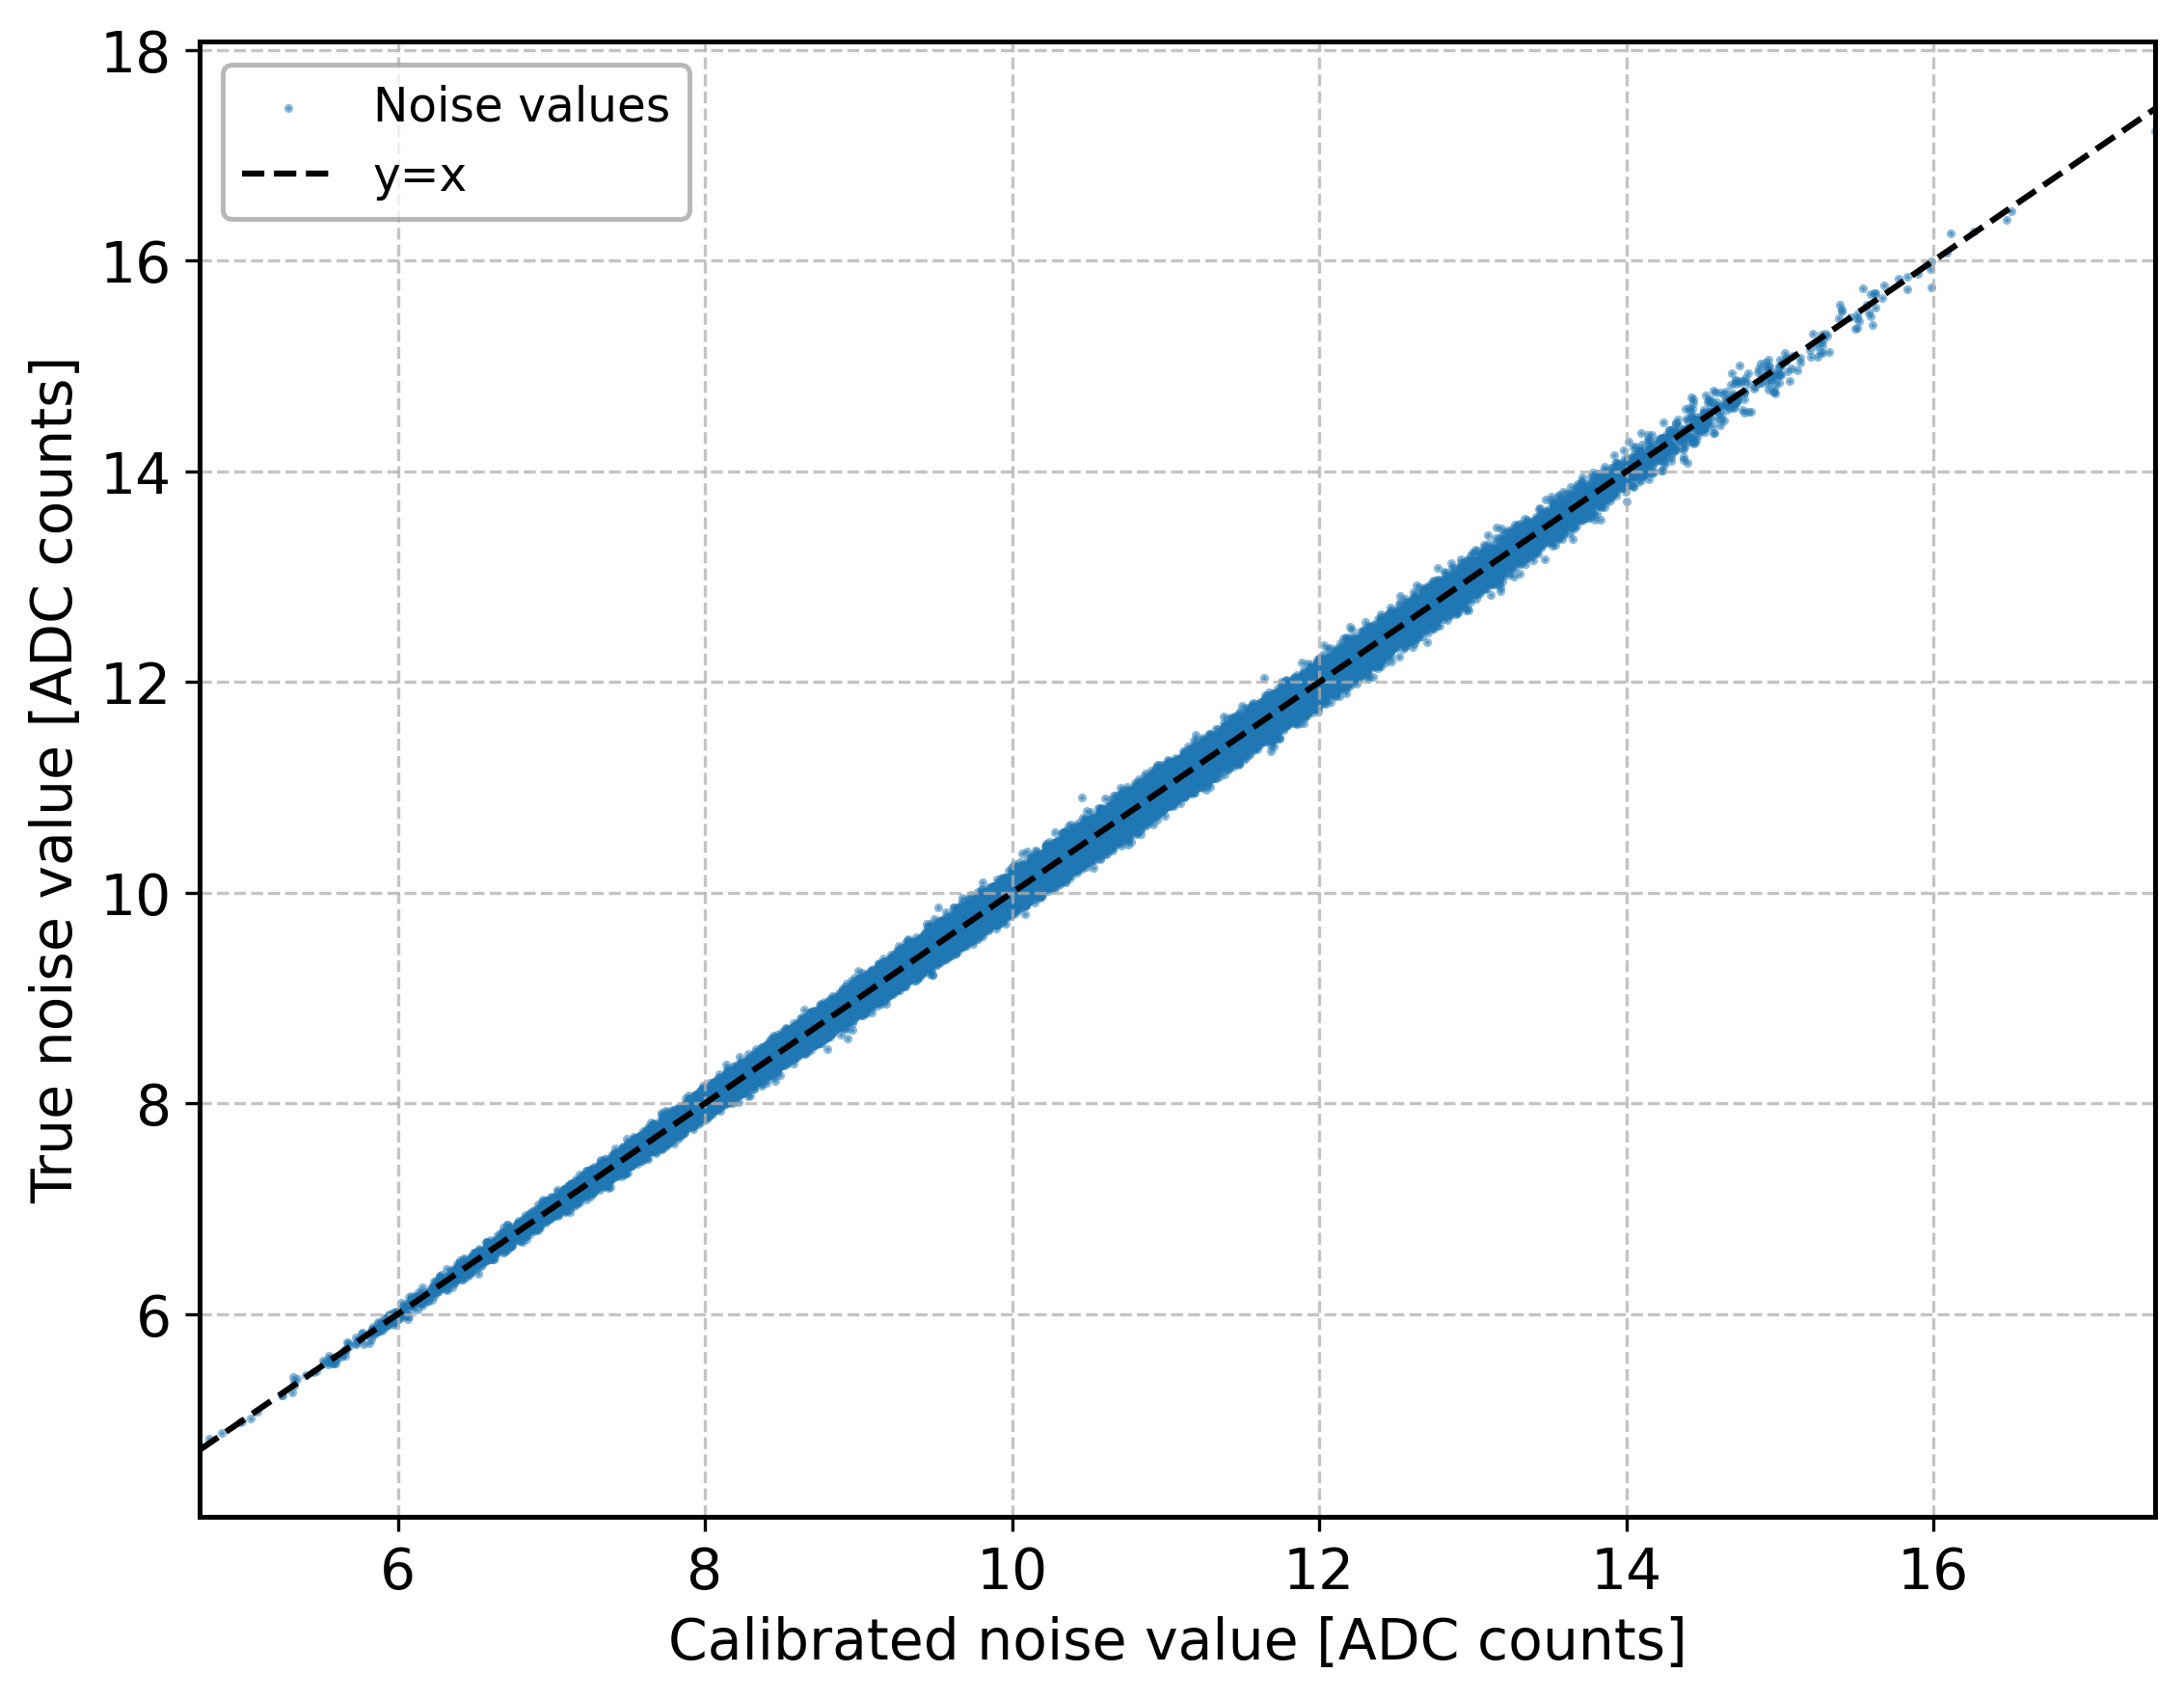
\includegraphics[width=0.49\linewidth]{figures/chapter4/calibration/noise_correlation}
    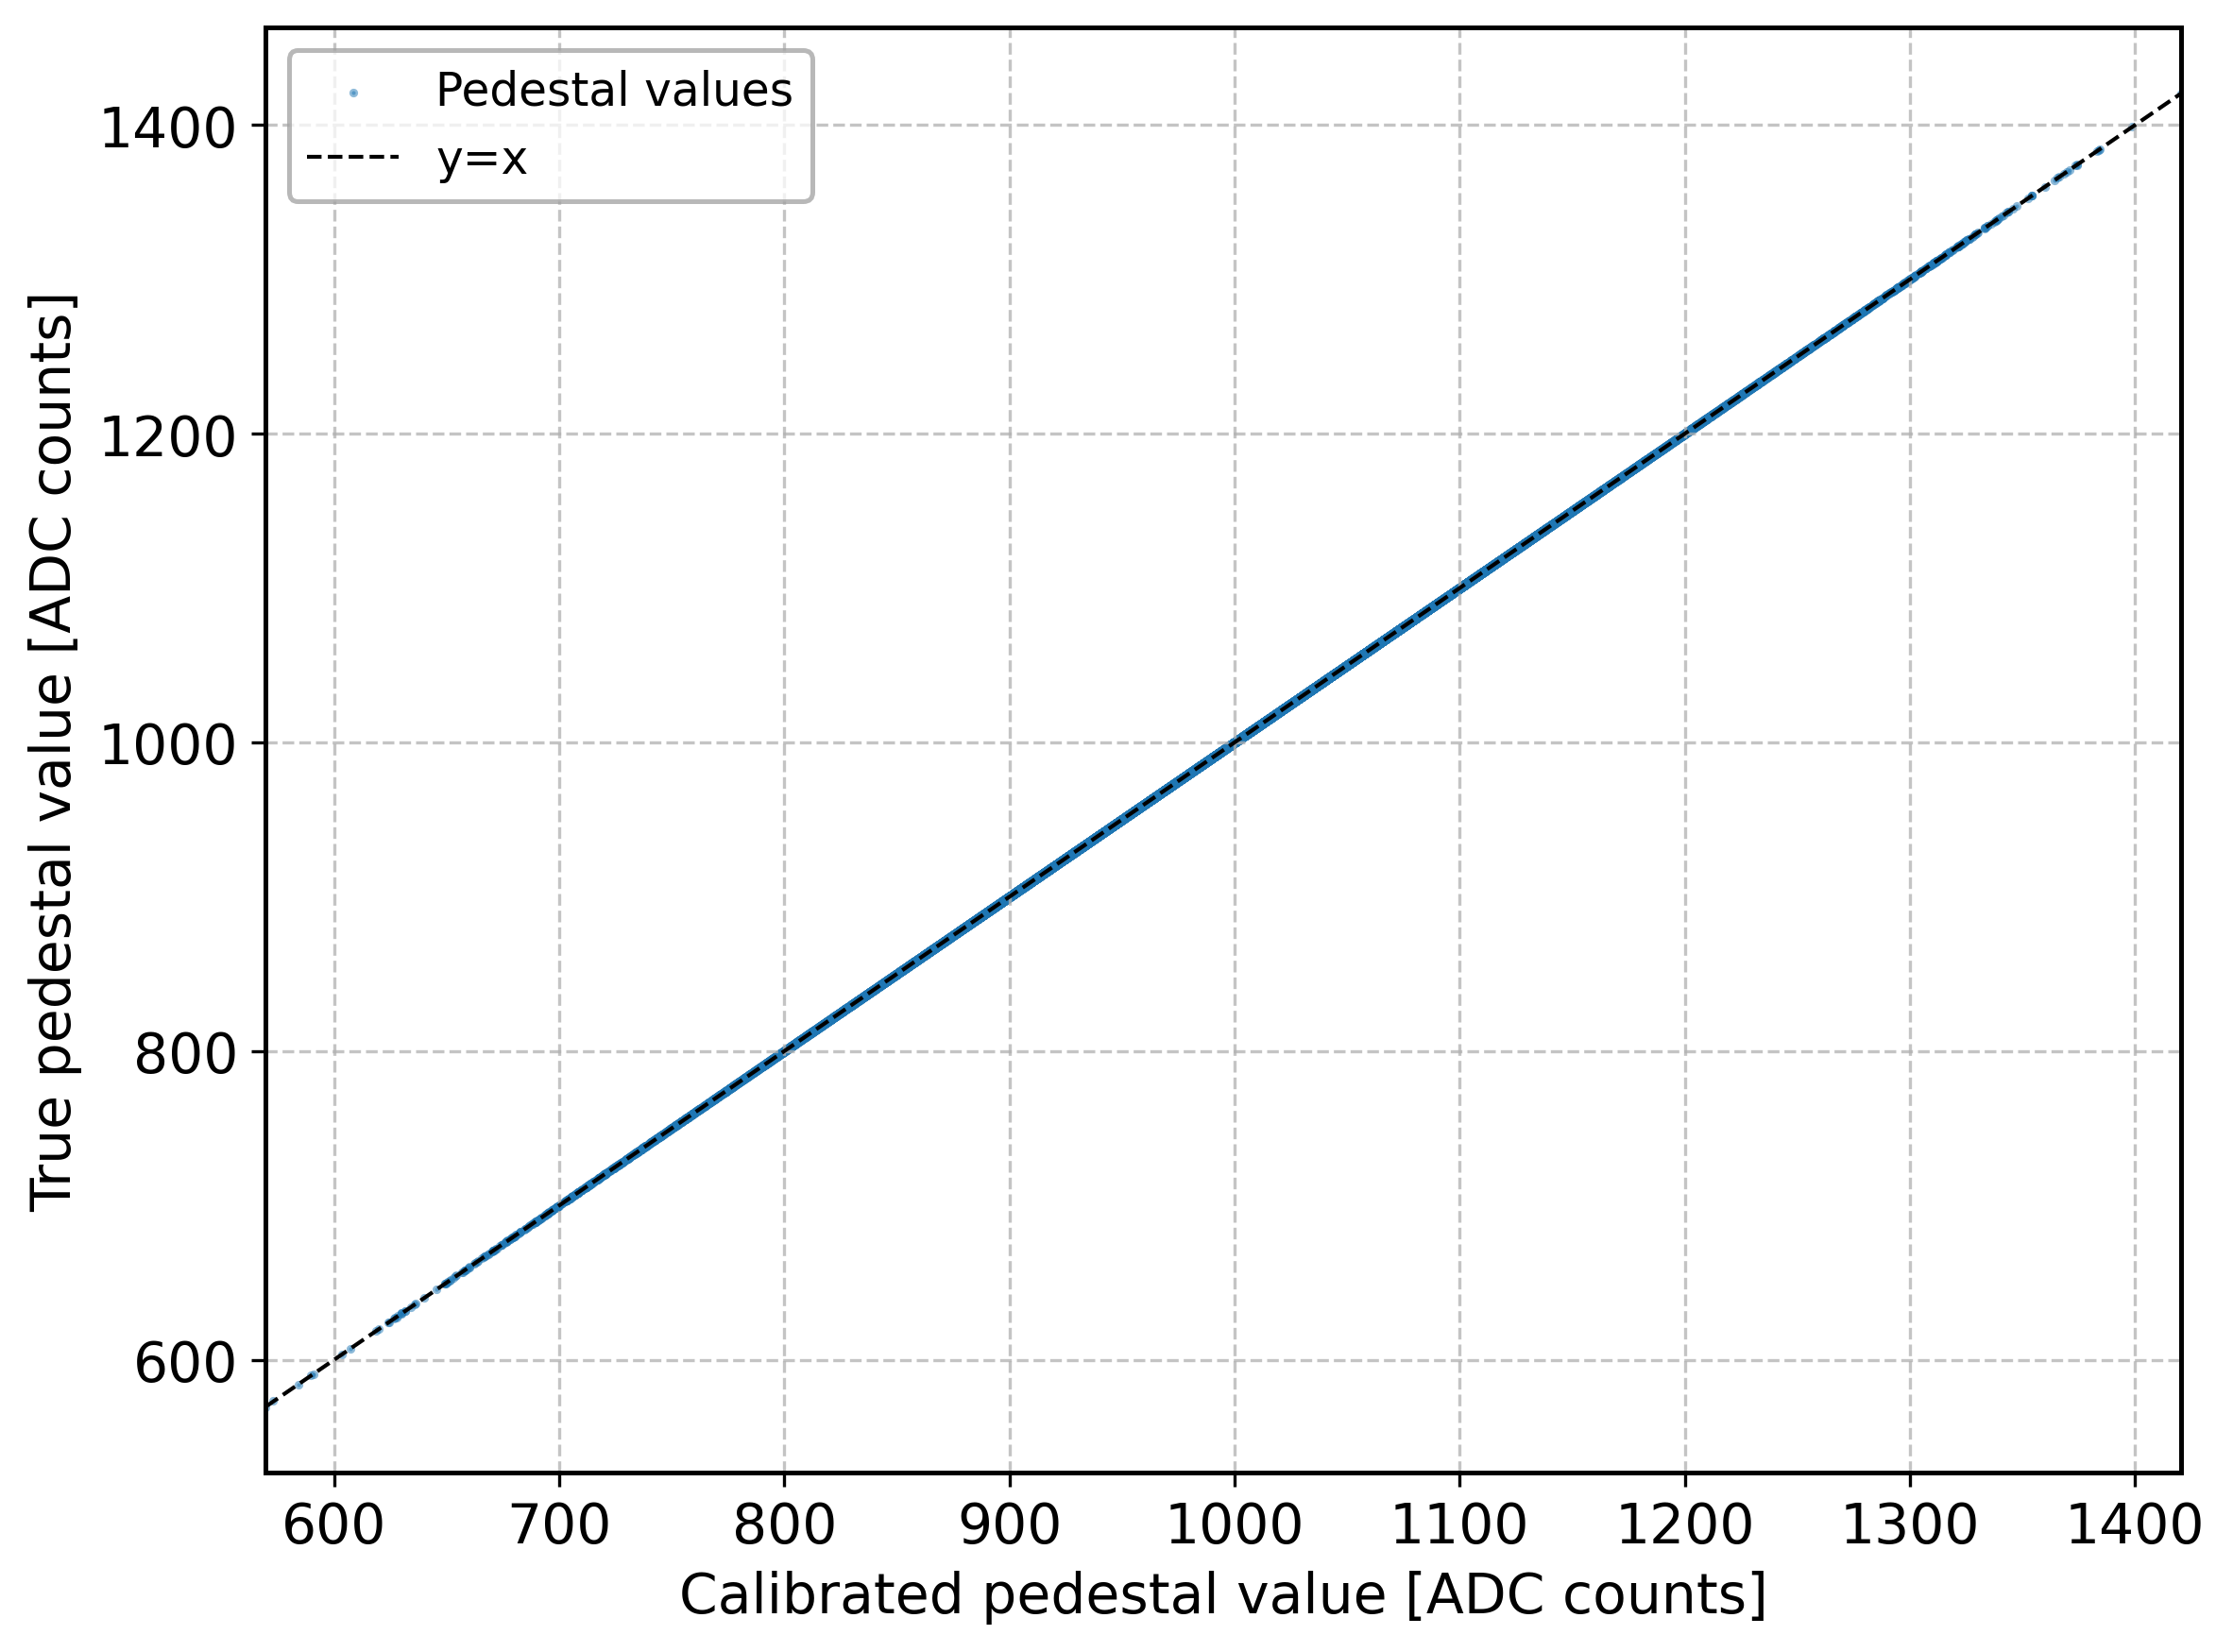
\includegraphics[width=0.49\linewidth]{figures/chapter4/calibration/pedestal_correlation}
    \caption{Two-dimensional correlation histograms between the true Monte Carlo values and the calibrated values for pixel noise (left) and pedestal levels (right). The red dashed line represents the ideal $y = x$ correlation.}
    \label{fig:noise_pedestal}
\end{figure}

Fig. \ref{fig:noise_distribution} shows the distribution of the calibrated values of the noise matrix and the residuals distribution. The ADC noise distribution is not a Gaussian because it is the product of two random variables, the ENC and gain, distributed according two different Gaussian distributions. The resulting distribution is a more complex skewed distribution, with mean equal to the product of the means of the parent distributions \cite{aroian1947}.

The residuals distribution has a standard deviation of about 0.07 ADC, equal to a mean relative error on the calibrated pixel value of 0.7\%, which is compatible with the expected relative error estimated from Eq. \ref{eq:noise_uncertainty} using the average number of events per pixel, which is about 11000 events.

Analogous results have been obtained for the pedestal calibration, whose residuals distribution has a standard deviation of 0.1 ADC, compatible with the expected value estimated from Eq. \ref{eq:noise_uncertainty}.

\begin{figure}
    \centering
    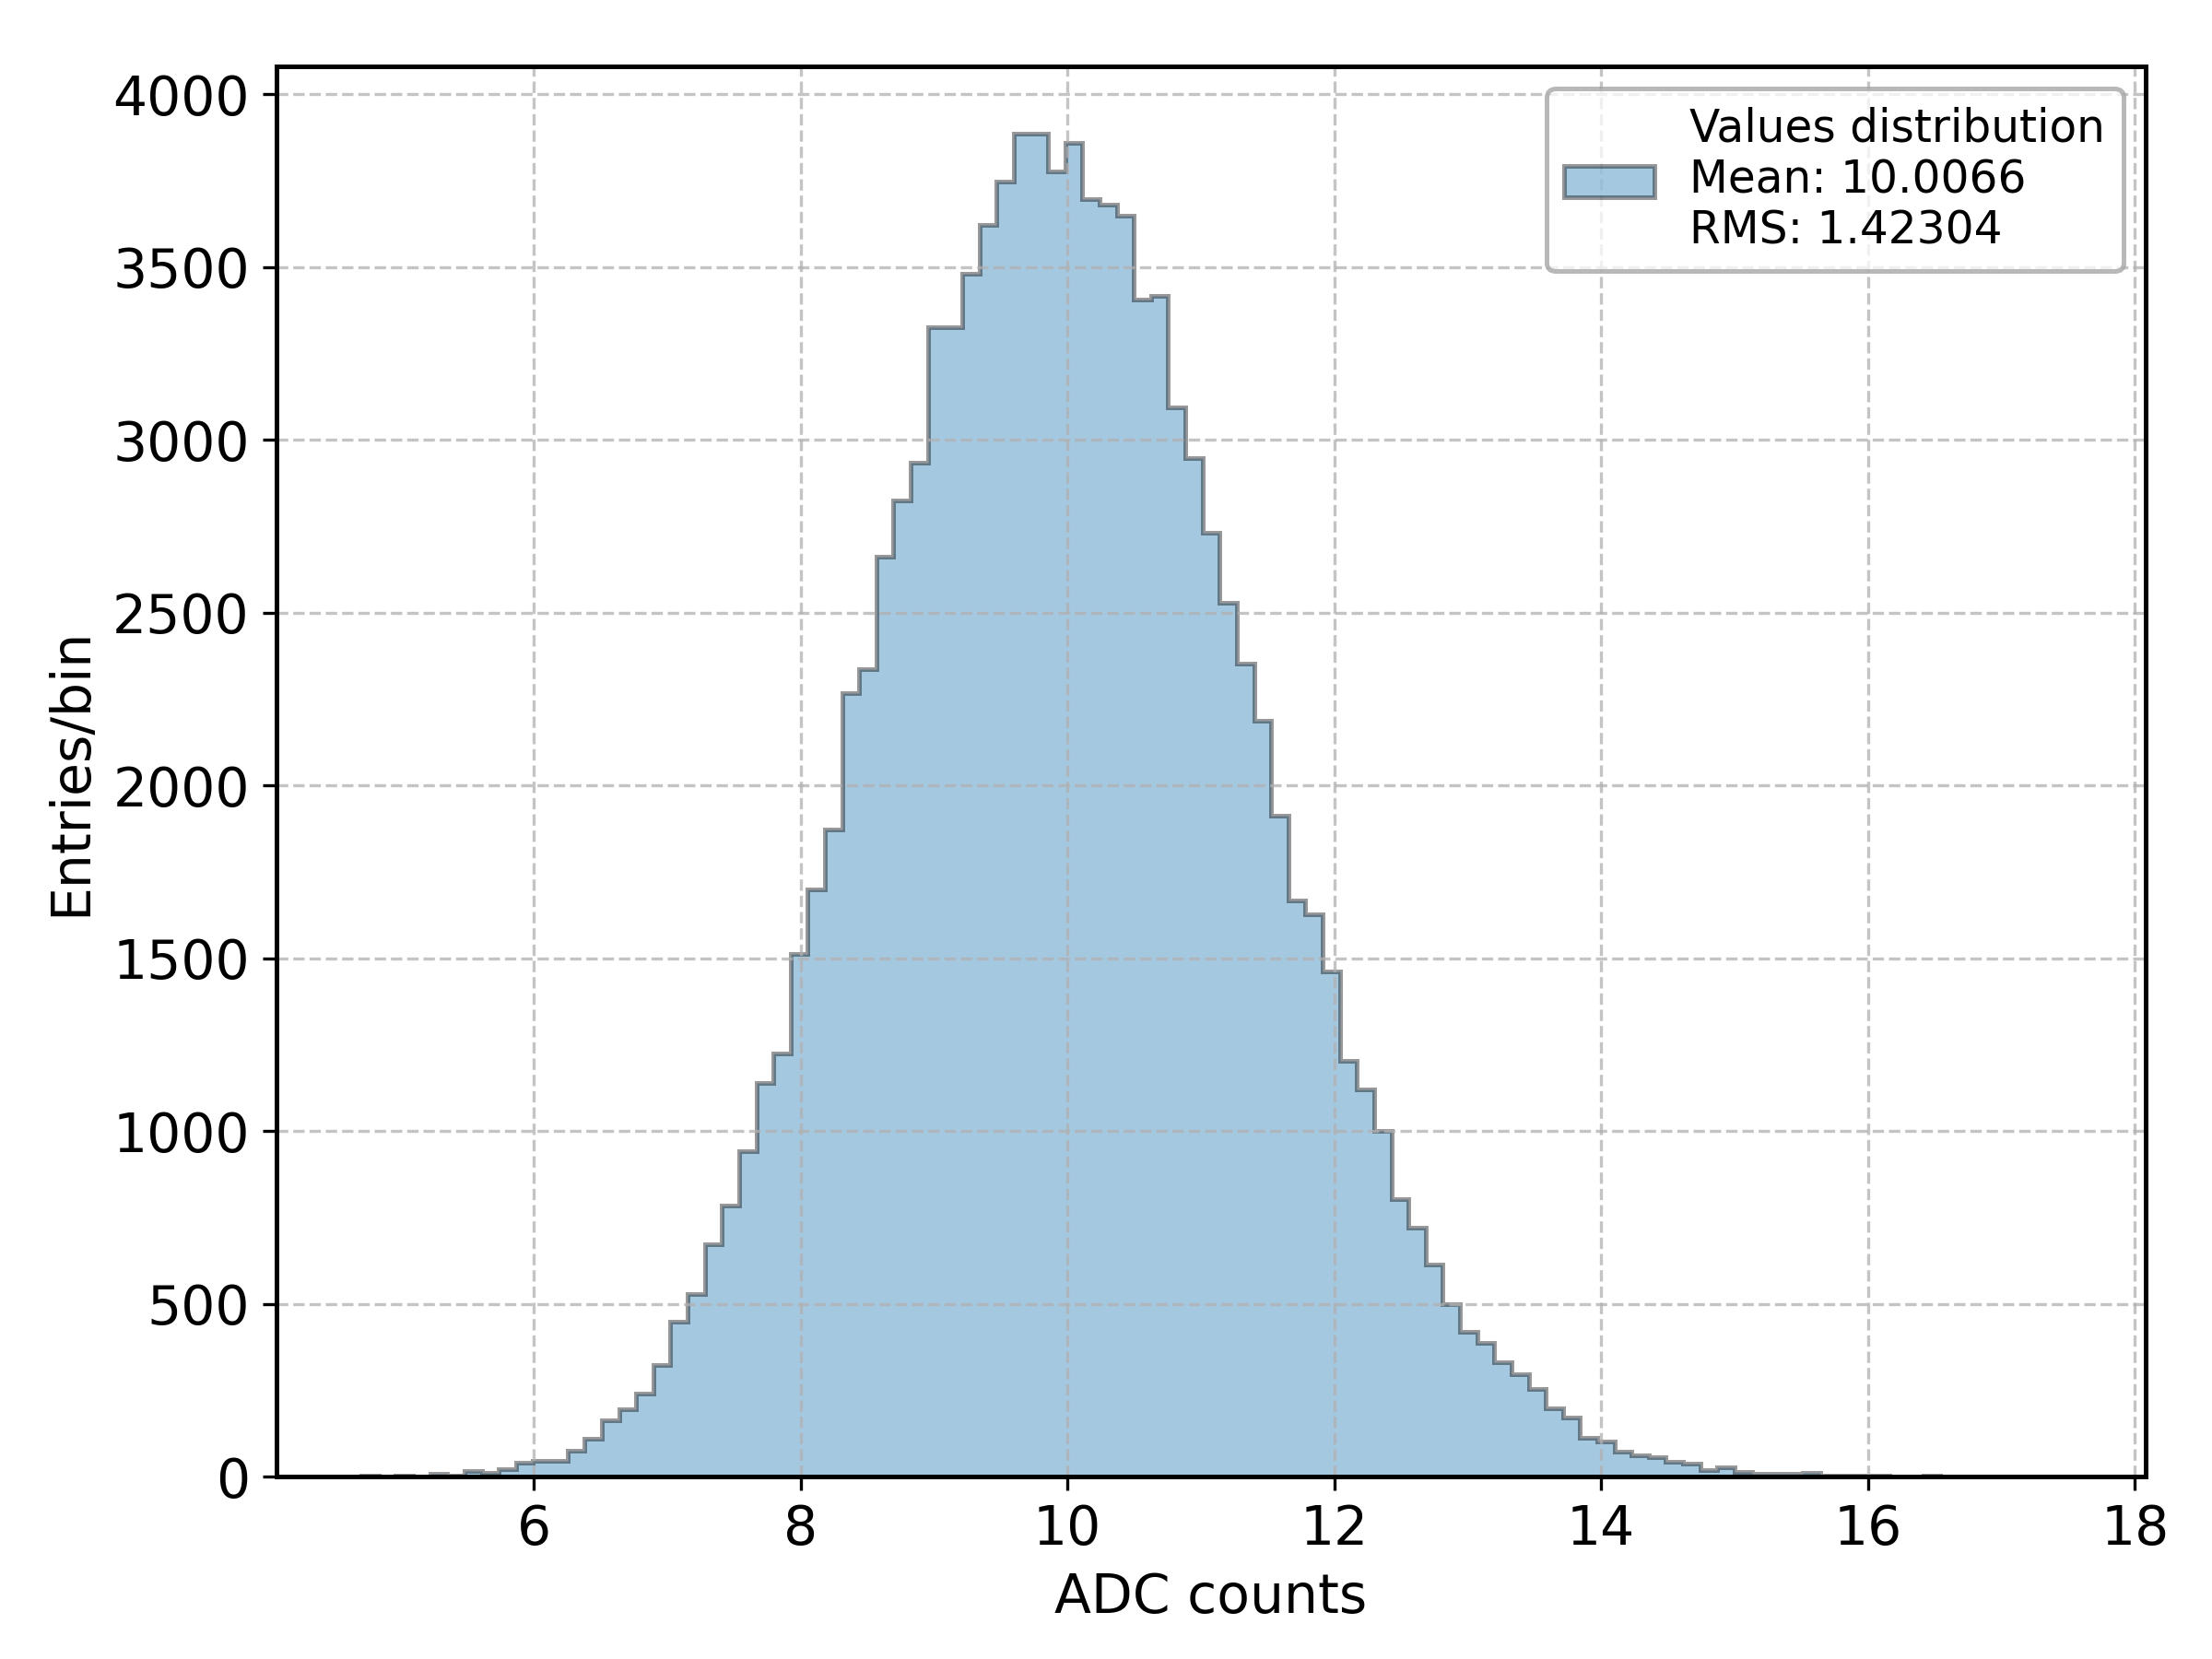
\includegraphics[width=0.49\linewidth]{figures/chapter4/noise_matrix_distribution}
    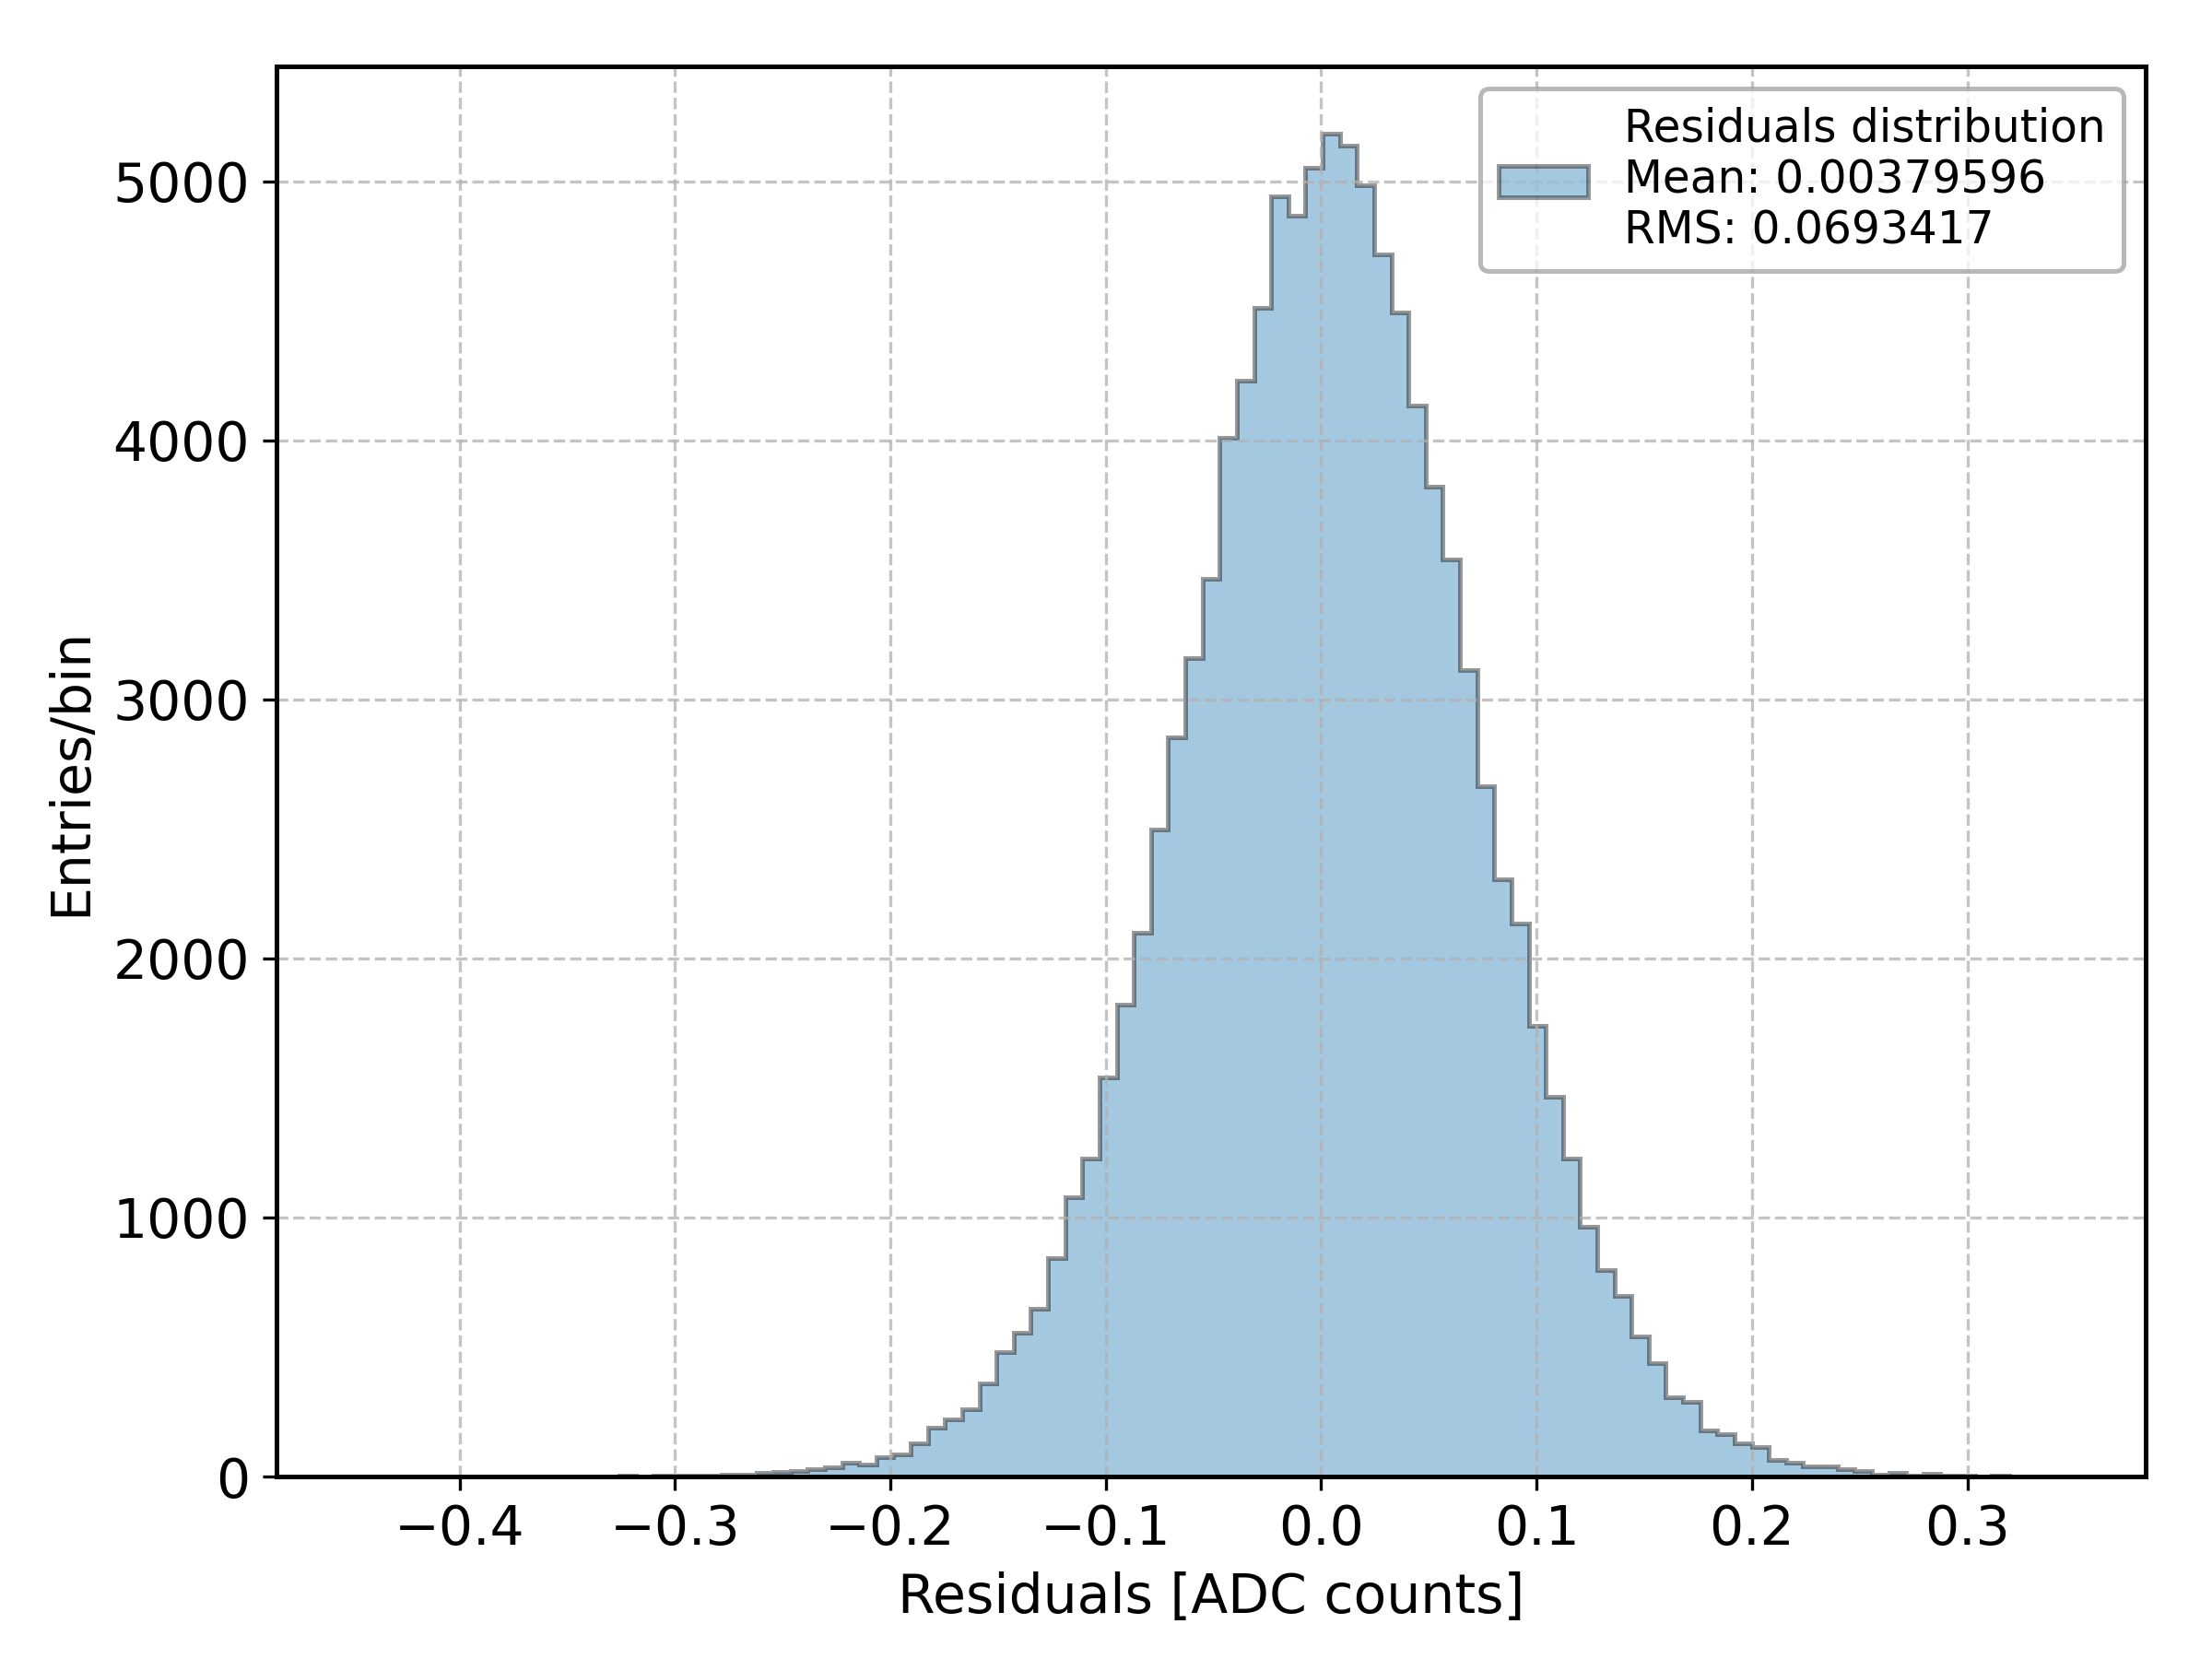
\includegraphics[width=0.49\linewidth]{figures/chapter4/noise_matrix_residuals}
    \caption{The left panel shows the calibrated values distribution of ADC noise, which is not a Gaussian distribution, but a distribution with a positive skewness. The residuals distribution is visible in the right panel.}
    \label{fig:noise_distribution}
\end{figure}

With these two calibration files, it is now possible to re-analyze the same dataset to calibrate the normalized gain. Both algorithms described above have been tested. The first one is straightforward, as it only requires using the noise and pedestal calibration products to remove offsets and correctly weight the pixel contents. However, with this method, only about 6\% of all events are classifiable as one-pixel events and can be used for the calibration, meaning that on average each pixel collects only about 6 events.

The second method requires running a simulation of the source spectrum using the noise and pedestal calibration products and assuming a uniform gain across the chip (the exact value is relevant only for the absolute gain; thus, for the normalized gain, it can be set to 1). The simulated dataset is then reconstructed, and the resulting spectrum is used as the probability density function for the likelihood estimation of the normalized gain. This method exploits all events, resulting in an average of about 230 events per pixel.

The correlation between the true and the calibrated values of the normalized gain for the two methods is shown in Fig. \ref{fig:gain_results}. In both cases, the reconstructed values are well aligned along the $y=x$ identity line, demonstrating that both calibration procedures are unbiased and correctly reconstruct the normalized gain.

However, the two distributions show significant differences in terms of dispersion. The first method, being limited to one-pixel events with an average of only $\approx 6$ events per pixel, exhibits a broader distribution around the diagonal due to larger statistical fluctuations. In contrast, the second method exploits the full event statistics, resulting in a substantially narrower correlation band and thus a higher precision in the gain estimation. A very small fraction of outliers can be observed in the second method near the axes, corresponding to pixels where the likelihood minimization did not converge optimally. From the distribution of the residuals, the relative error on the normalized gain is found to be about 2\% for the first method and 1\% for the second method.

\begin{figure}
    \centering
    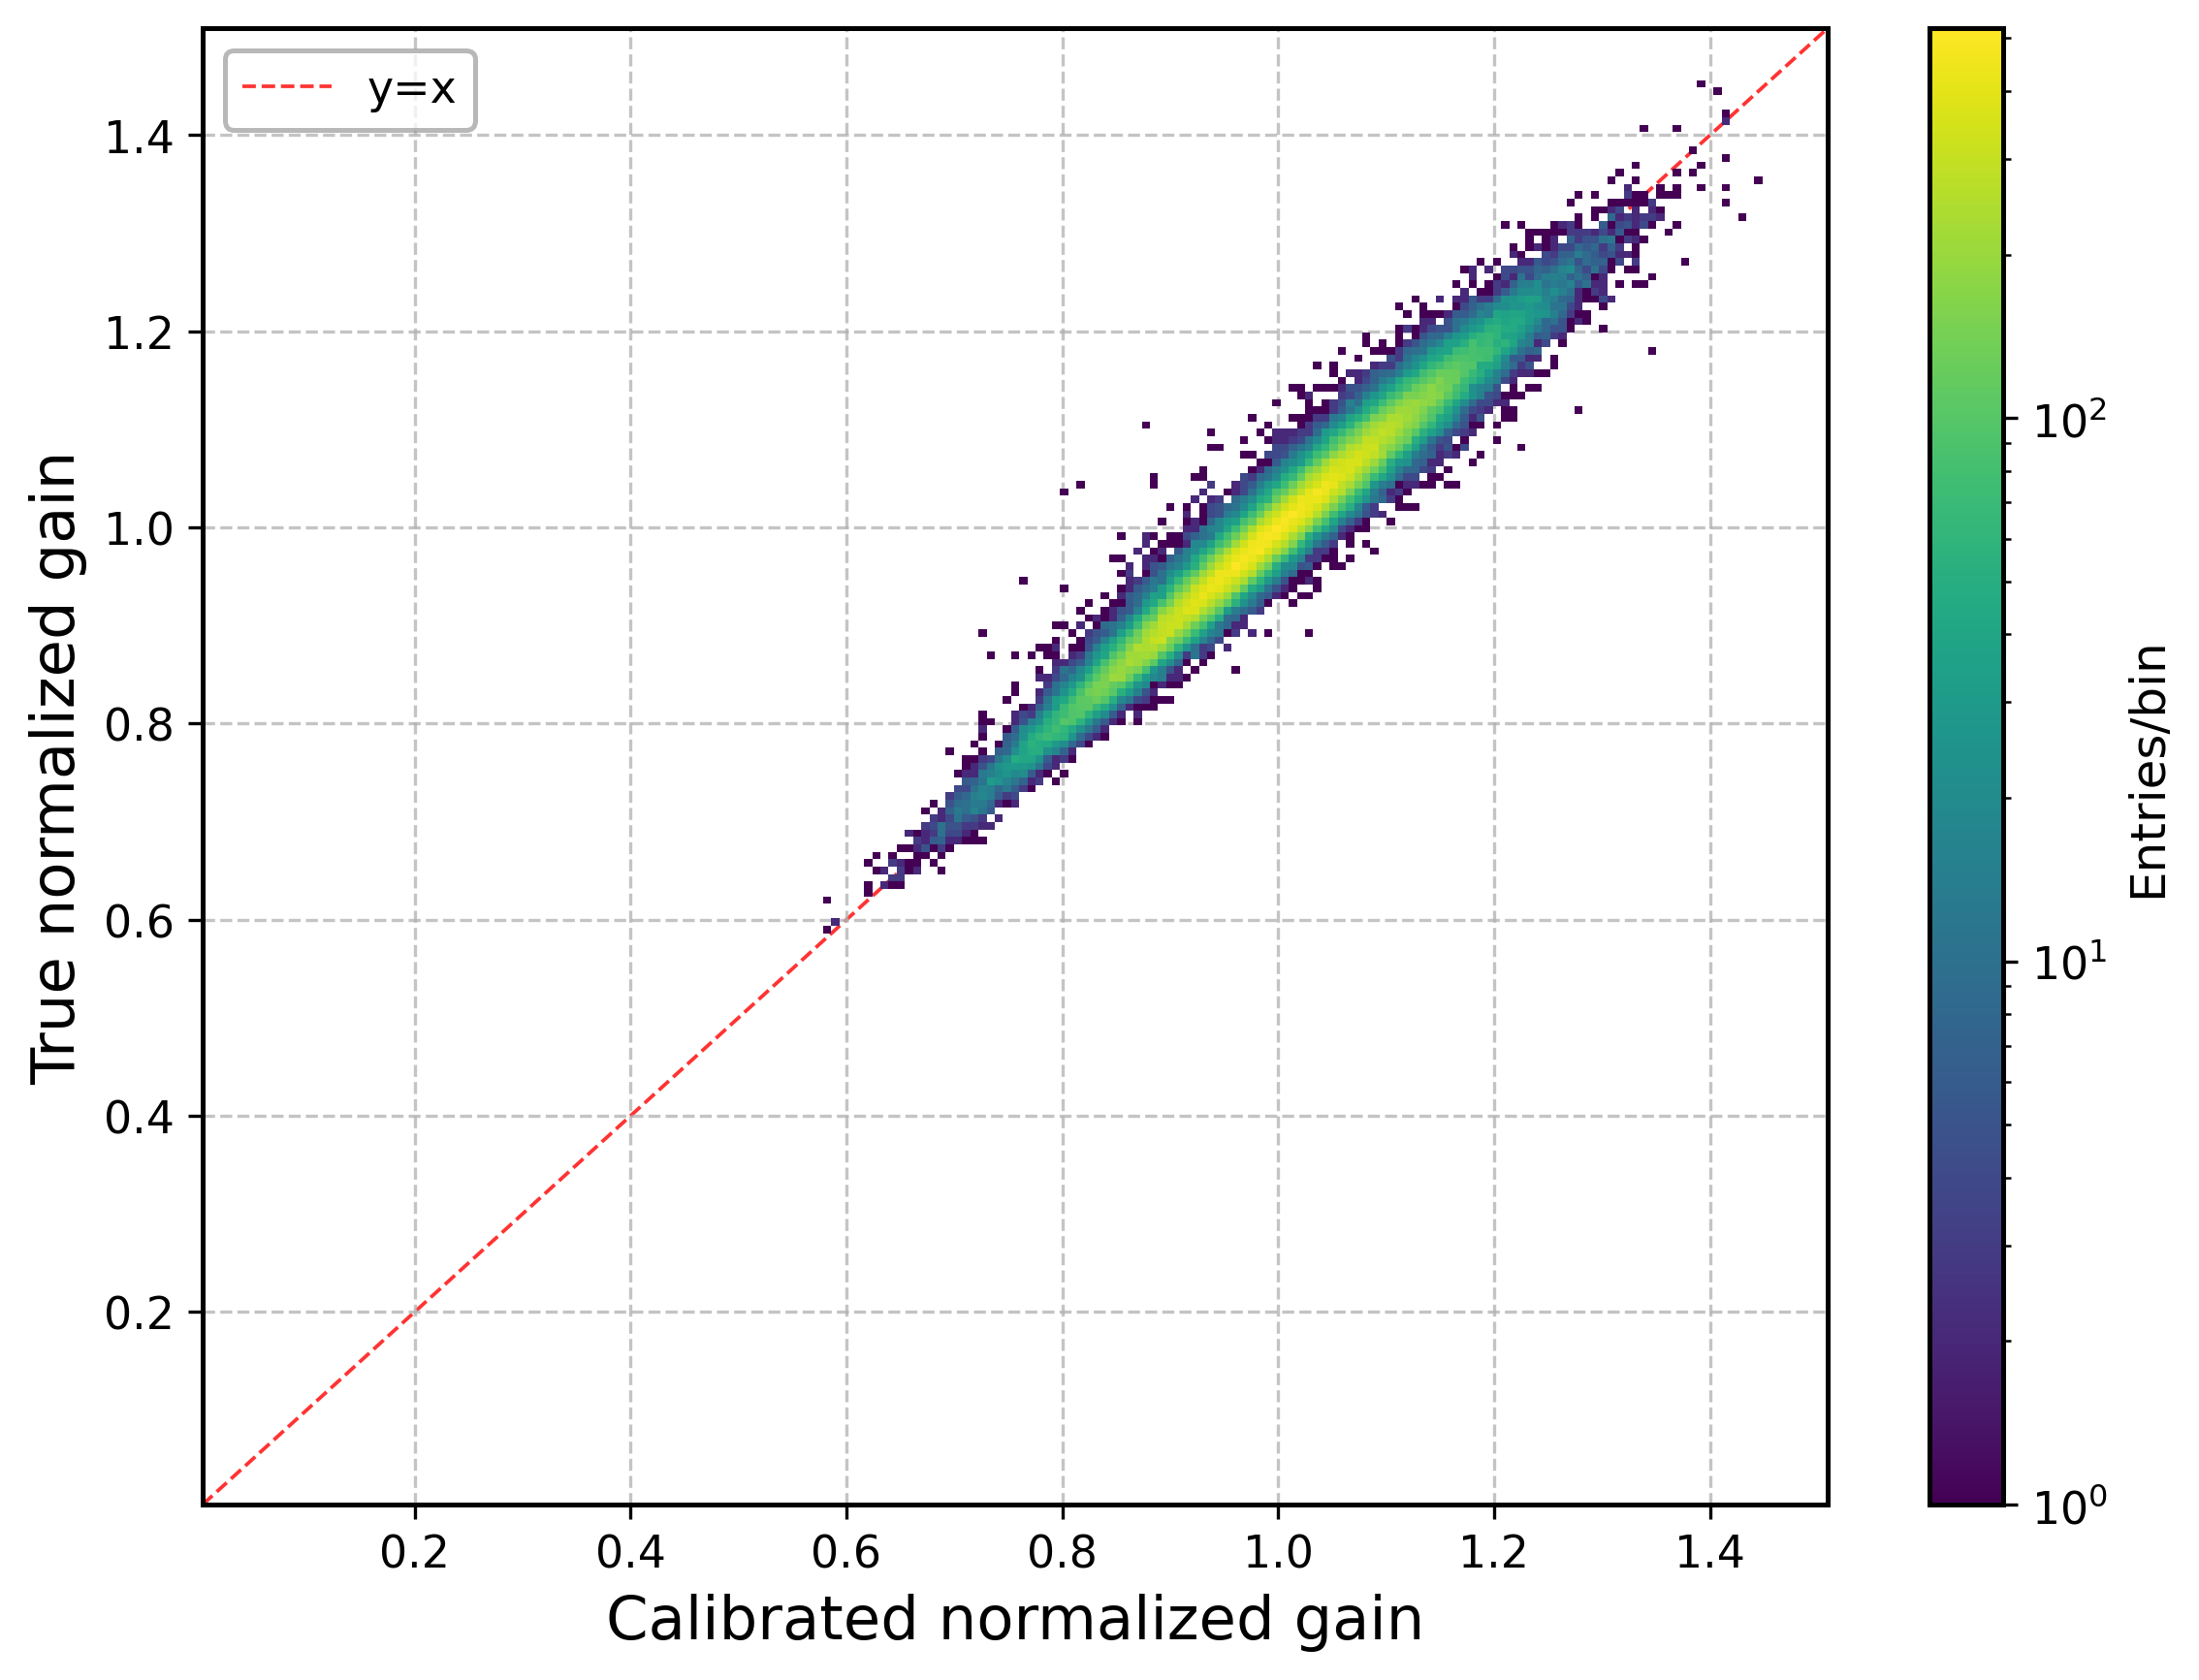
\includegraphics[width=0.49\linewidth]{figures/chapter4/calibration/equalization_correlation_method1}
    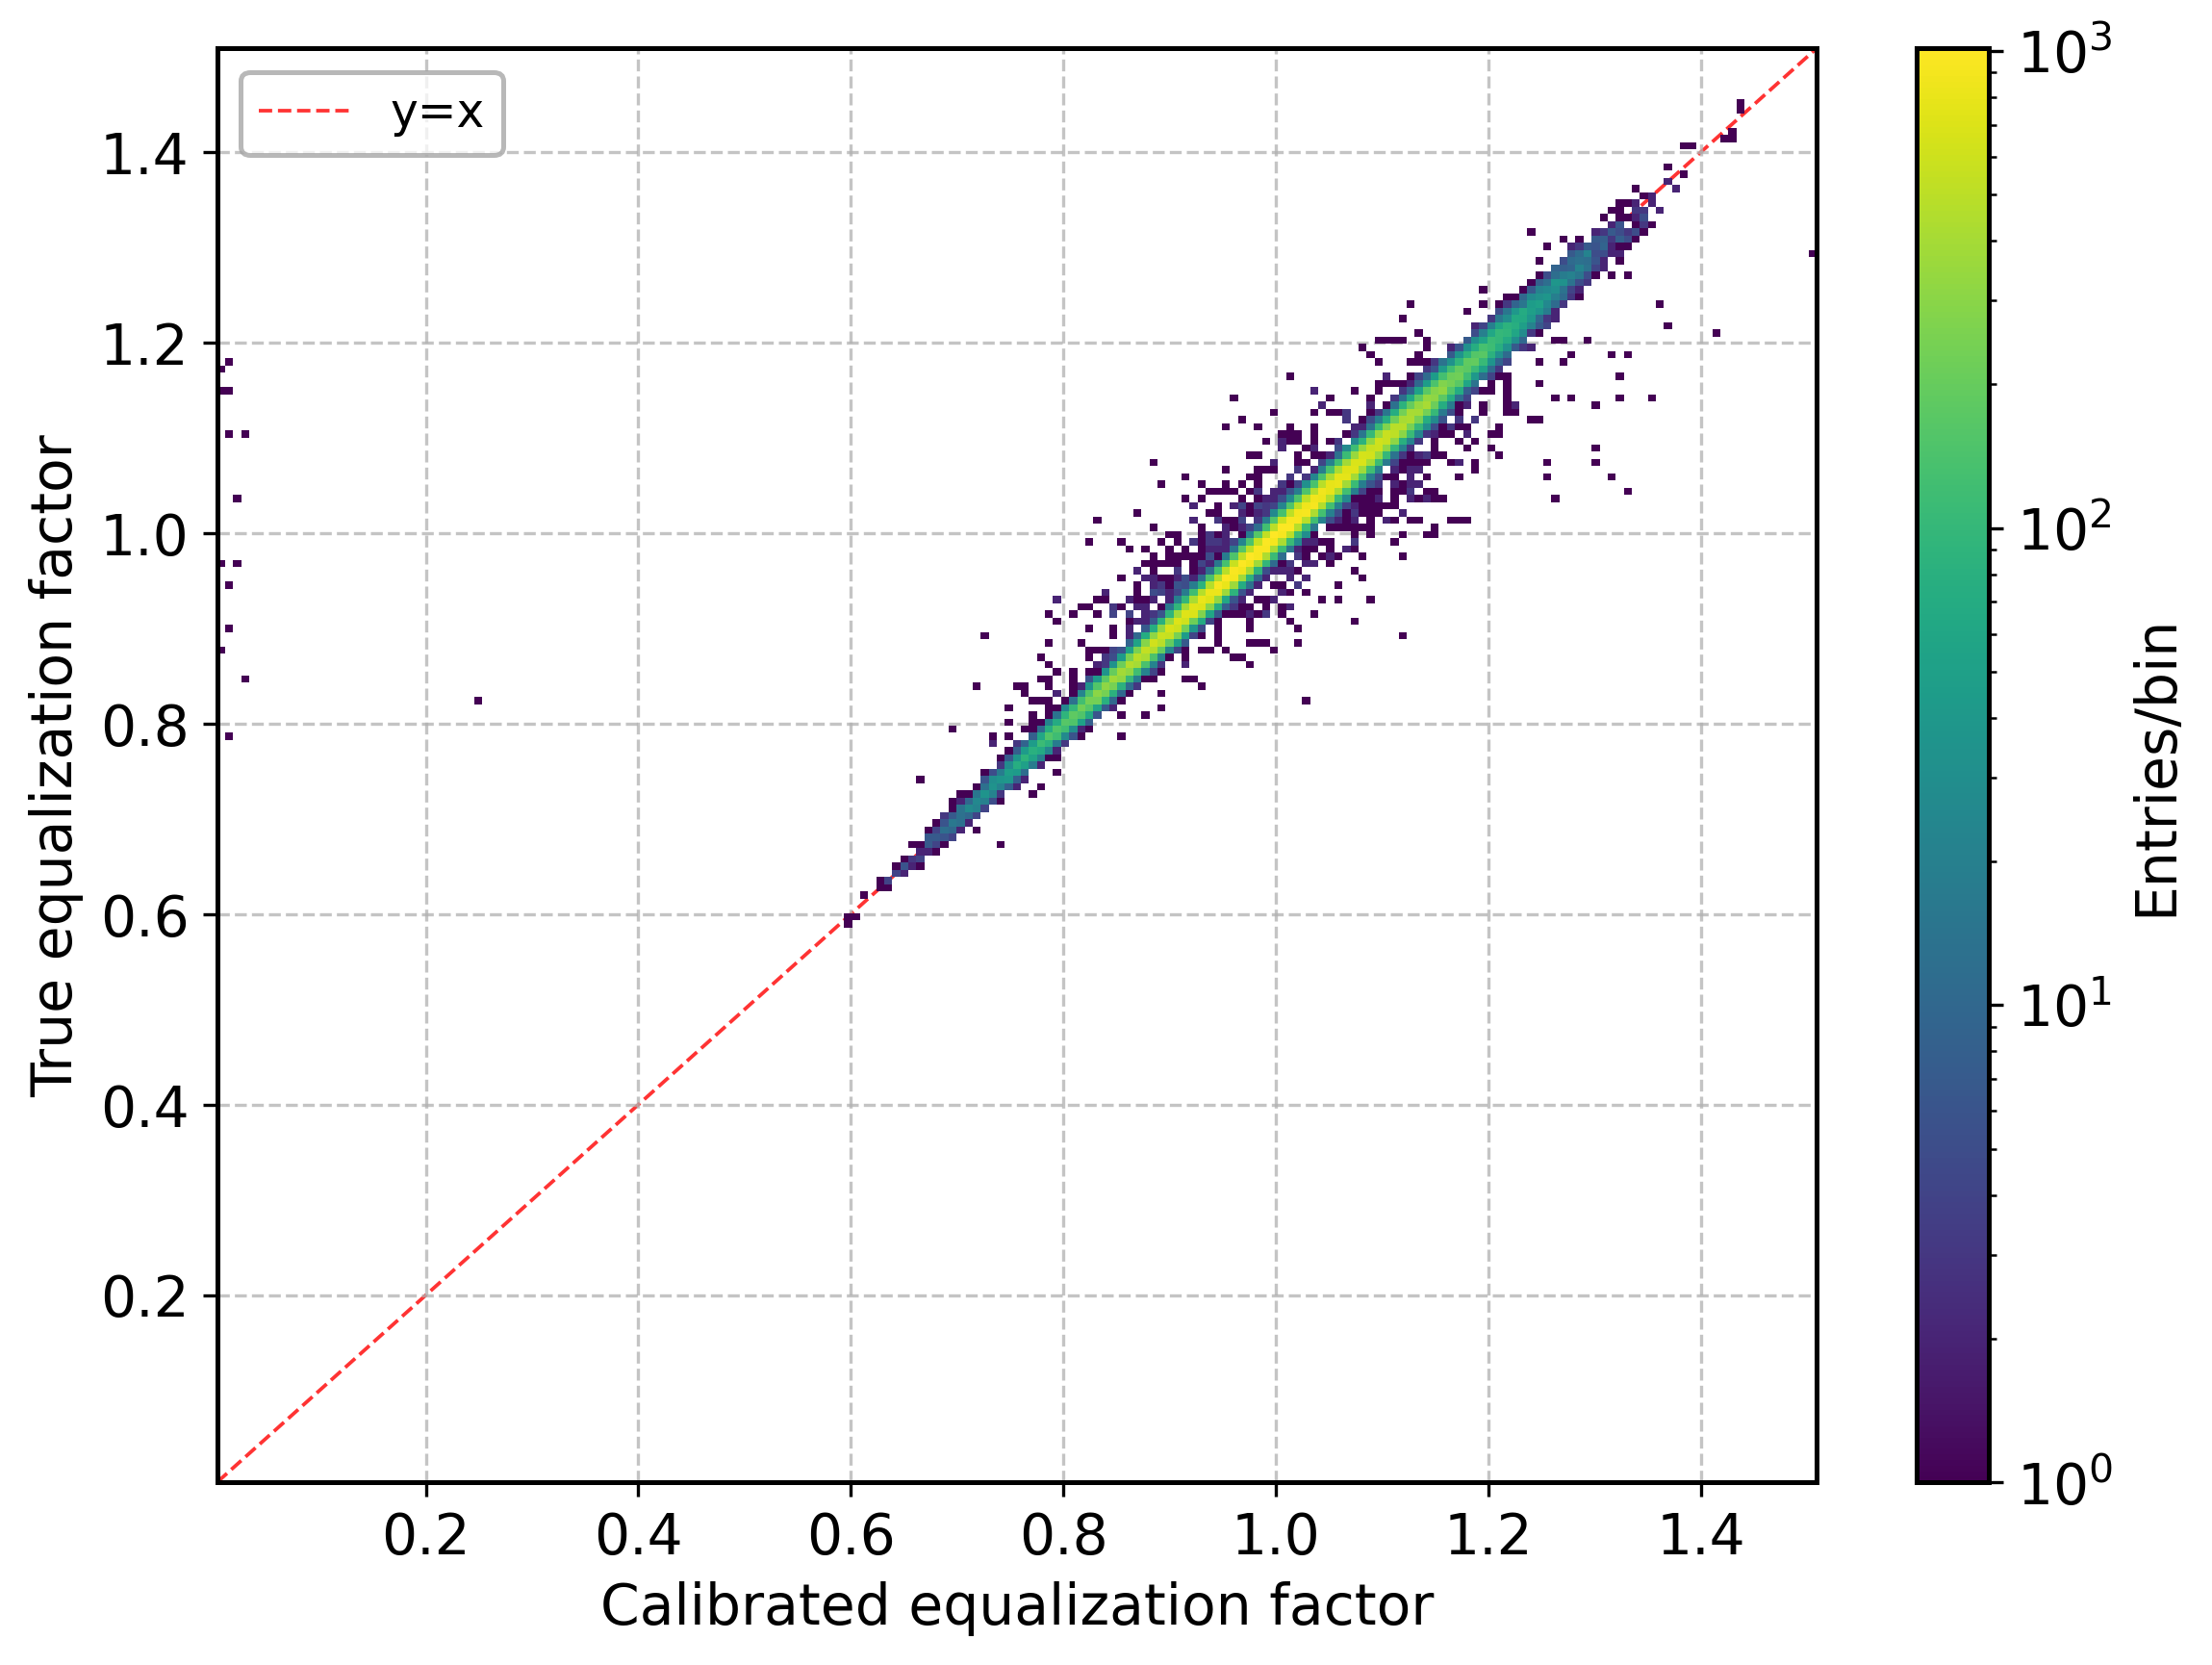
\includegraphics[width=0.49\linewidth]{figures/chapter4/calibration/equalization_correlation_method2}
    \caption{Two-dimensional correlation histograms between the calibrated equalization factors and the Monte Carlo truth for the one-pixel method (left) and the spectrum likelihood method (right). The red dashed line indicates the ideal $y = x$ correlation.}
    \label{fig:gain_results}
\end{figure}

\section{Position reconstruction}

With all the necessary calibration products, it is possible to reconstruct all the information about the events. The important thing to take into account is that one of the features of ASIX is that the size of the diffused charge cloud is a bit smaller than a pixel, meaning that the average cluster size is quite small, as shown in Chap. \ref{sec:asix_design}. While this feature is essential for spectroscopy, in order to minimize the contribution of noise, it introduces the need of a careful analysis to reconstruct the incident position.

As a consequence, different algorithms have been developed and compared to determine which one achieves the best spatial resolution. To estimate the performance of these algorithms, two distinct methods can be employed. 

The first approach is typical for space applications, where a source with a known spatial profile, such as a point-like source, is used to directly compare the true incidence position with the reconstructed one. In this work, this method is implemented using the Monte Carlo ground truth. The metric used to gauge the spatial resolution is the encircled energy fraction (EEF). The EEF is the cumulative density function of the radial distance distribution between the true and the reconstructed positions \cite{longair2011}.

Usually, the EEF is calculated by integrating the Point Spread Function (PSF), which represents the response of a detector to a point-like source. In this case, given the availability of the Monte Carlo ground truth positions, it can be directly derived from the radial residuals distribution. Common metrics of the EEF are the radii corresponding to 50\% (Half-Energy Width, HEW) and 90\% encircled energy, which represent the customary standard for space telescopes. The HEW measures the core spatial resolution, while the latter is sensitive to the extended tails of the distribution.

The second approach is standard in medical and industrial imaging and relies on evaluating the spatial response of the detector to an illuminated slit or a sharp edge. This method has been adopted to analyze laboratory experimental data.

\subsection{Charge barycenter}
\label{subsec:barycenter}

The simplest possible algorithm consists of calculating the barycenter of the pixels centers by weighting their positions with the collected charge

\begin{equation}
x = \frac{\sum_i x_i \cdot q_i}{\sum_i q_i}, \quad y = \frac{\sum_i y_i \cdot q_i}{\sum_i q_i},
\end{equation}
where $x_i$ and $y_i$ are the coordinates of the $i$-th pixel and $q_i$ is the charge collected by it.

\begin{figure}[!b]
    \centering
    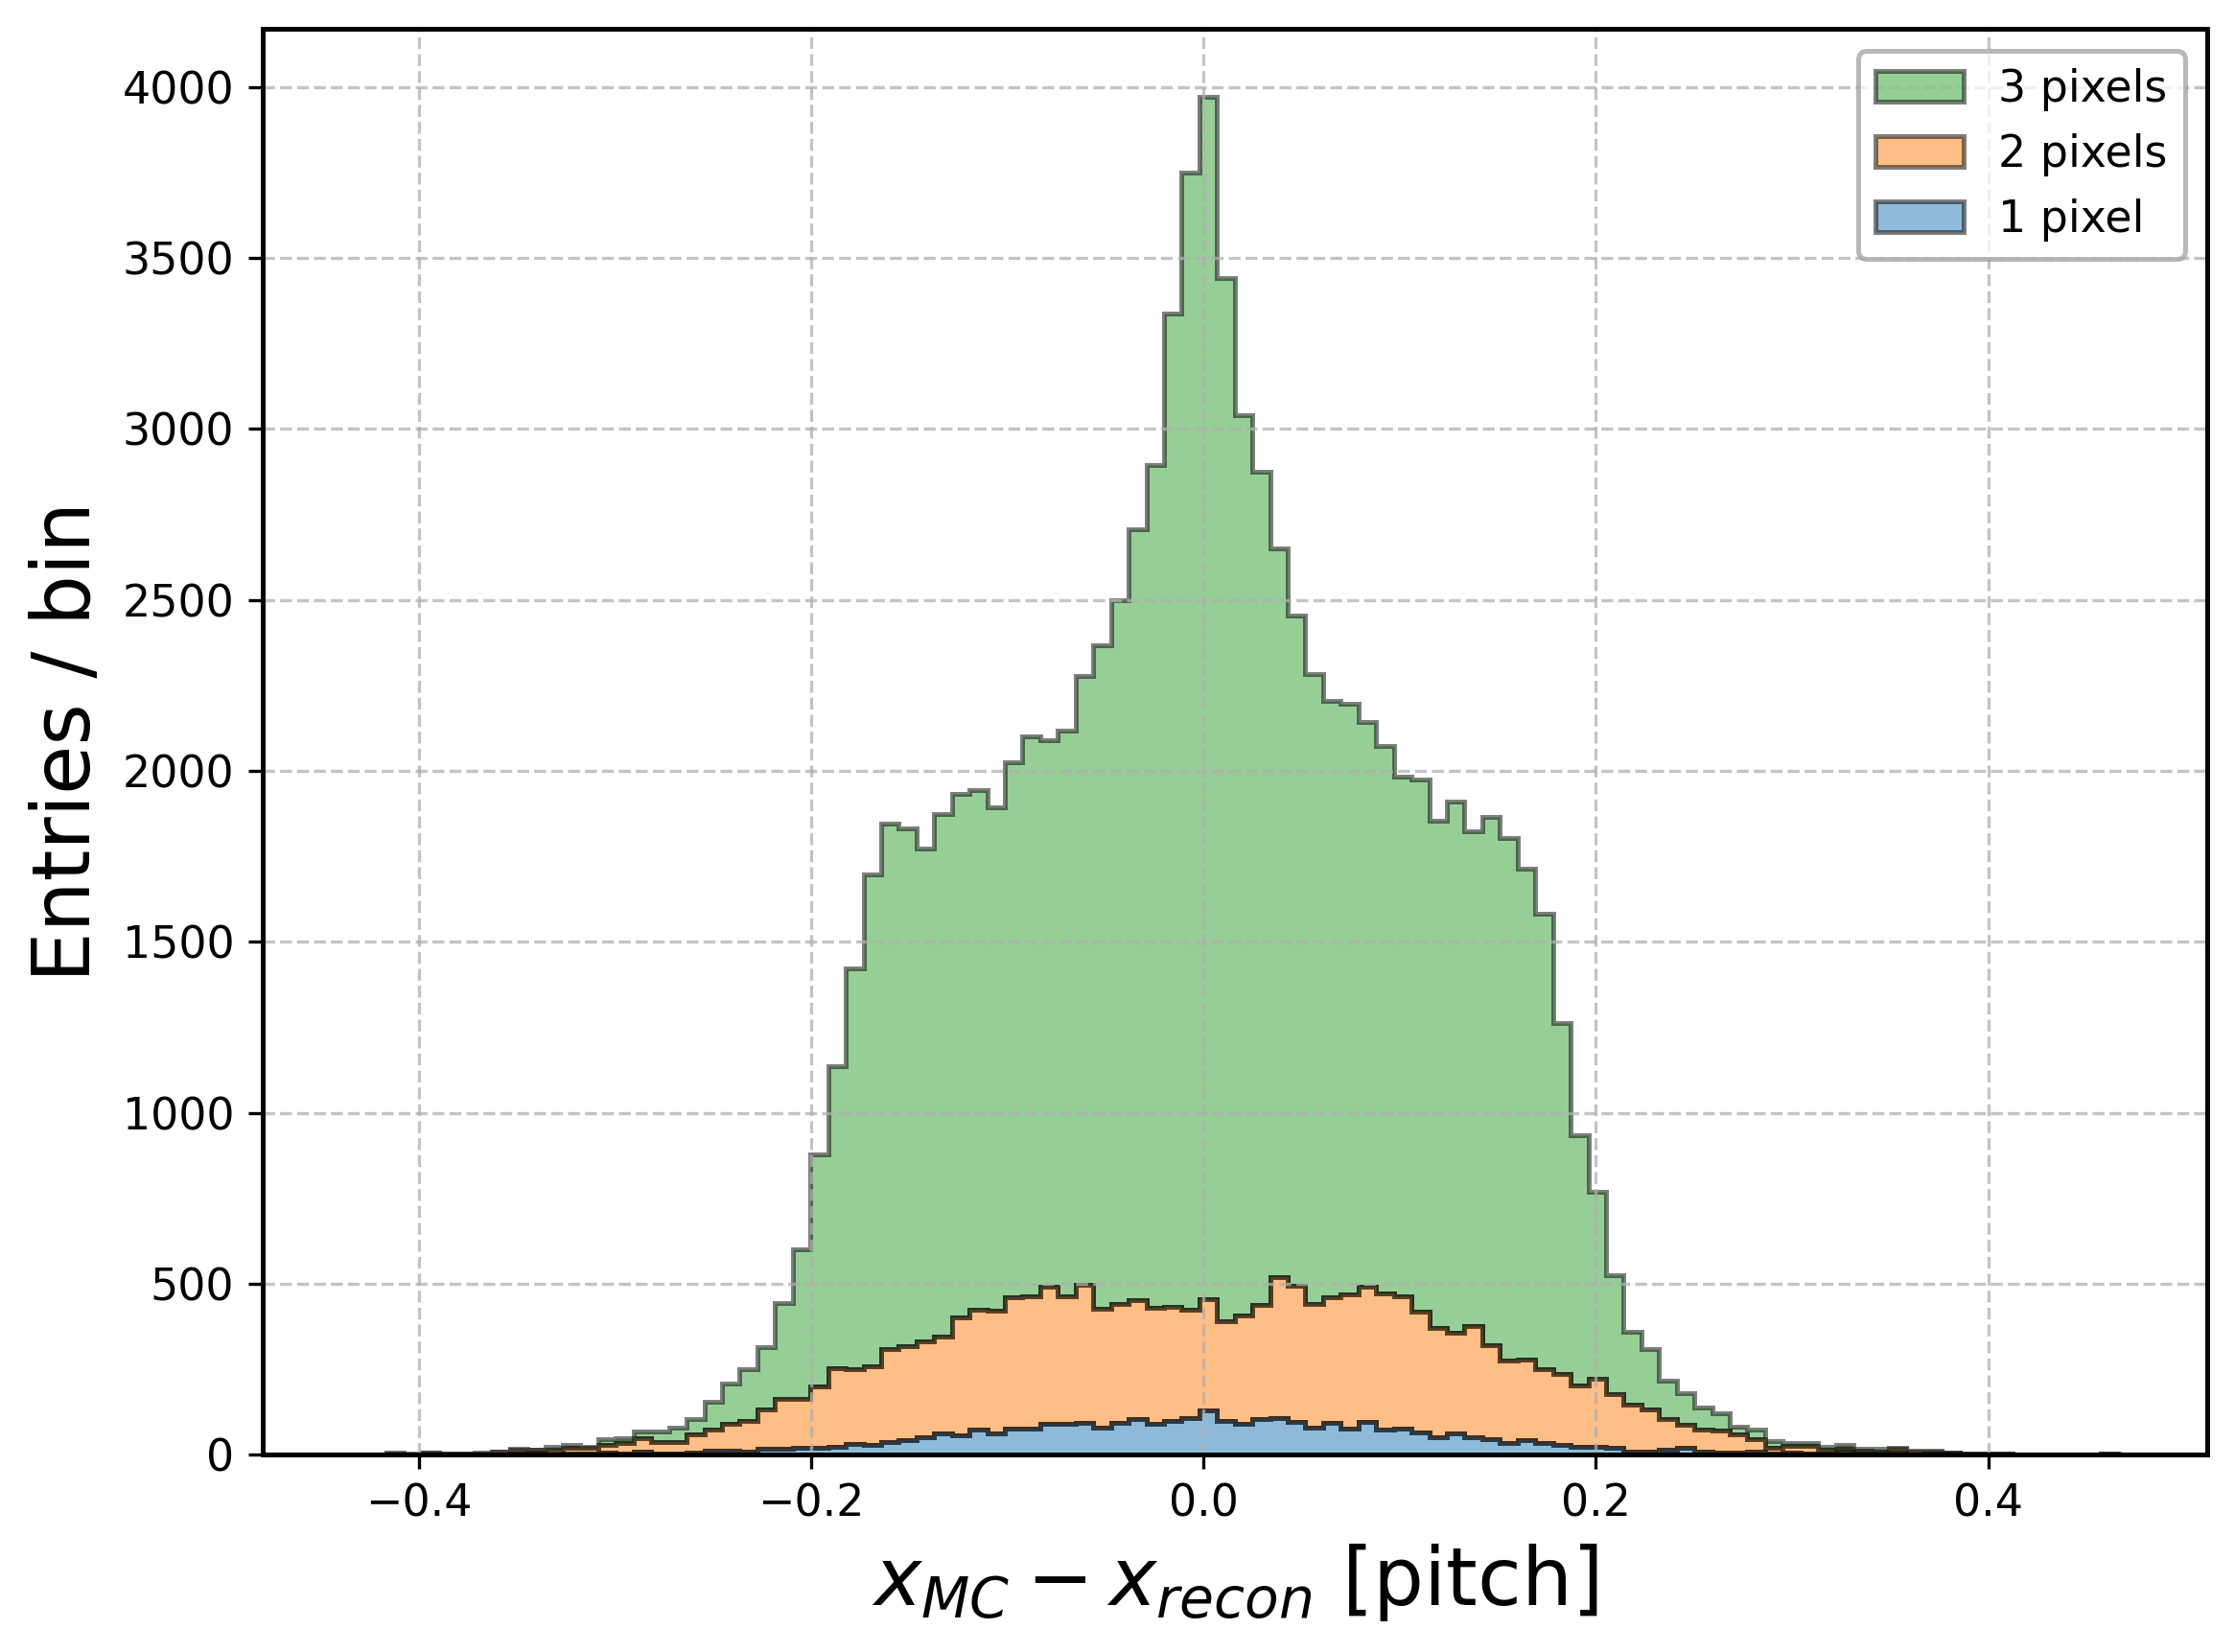
\includegraphics[width=0.49\linewidth]{figures/chapter4/position/barycenter_dx}
    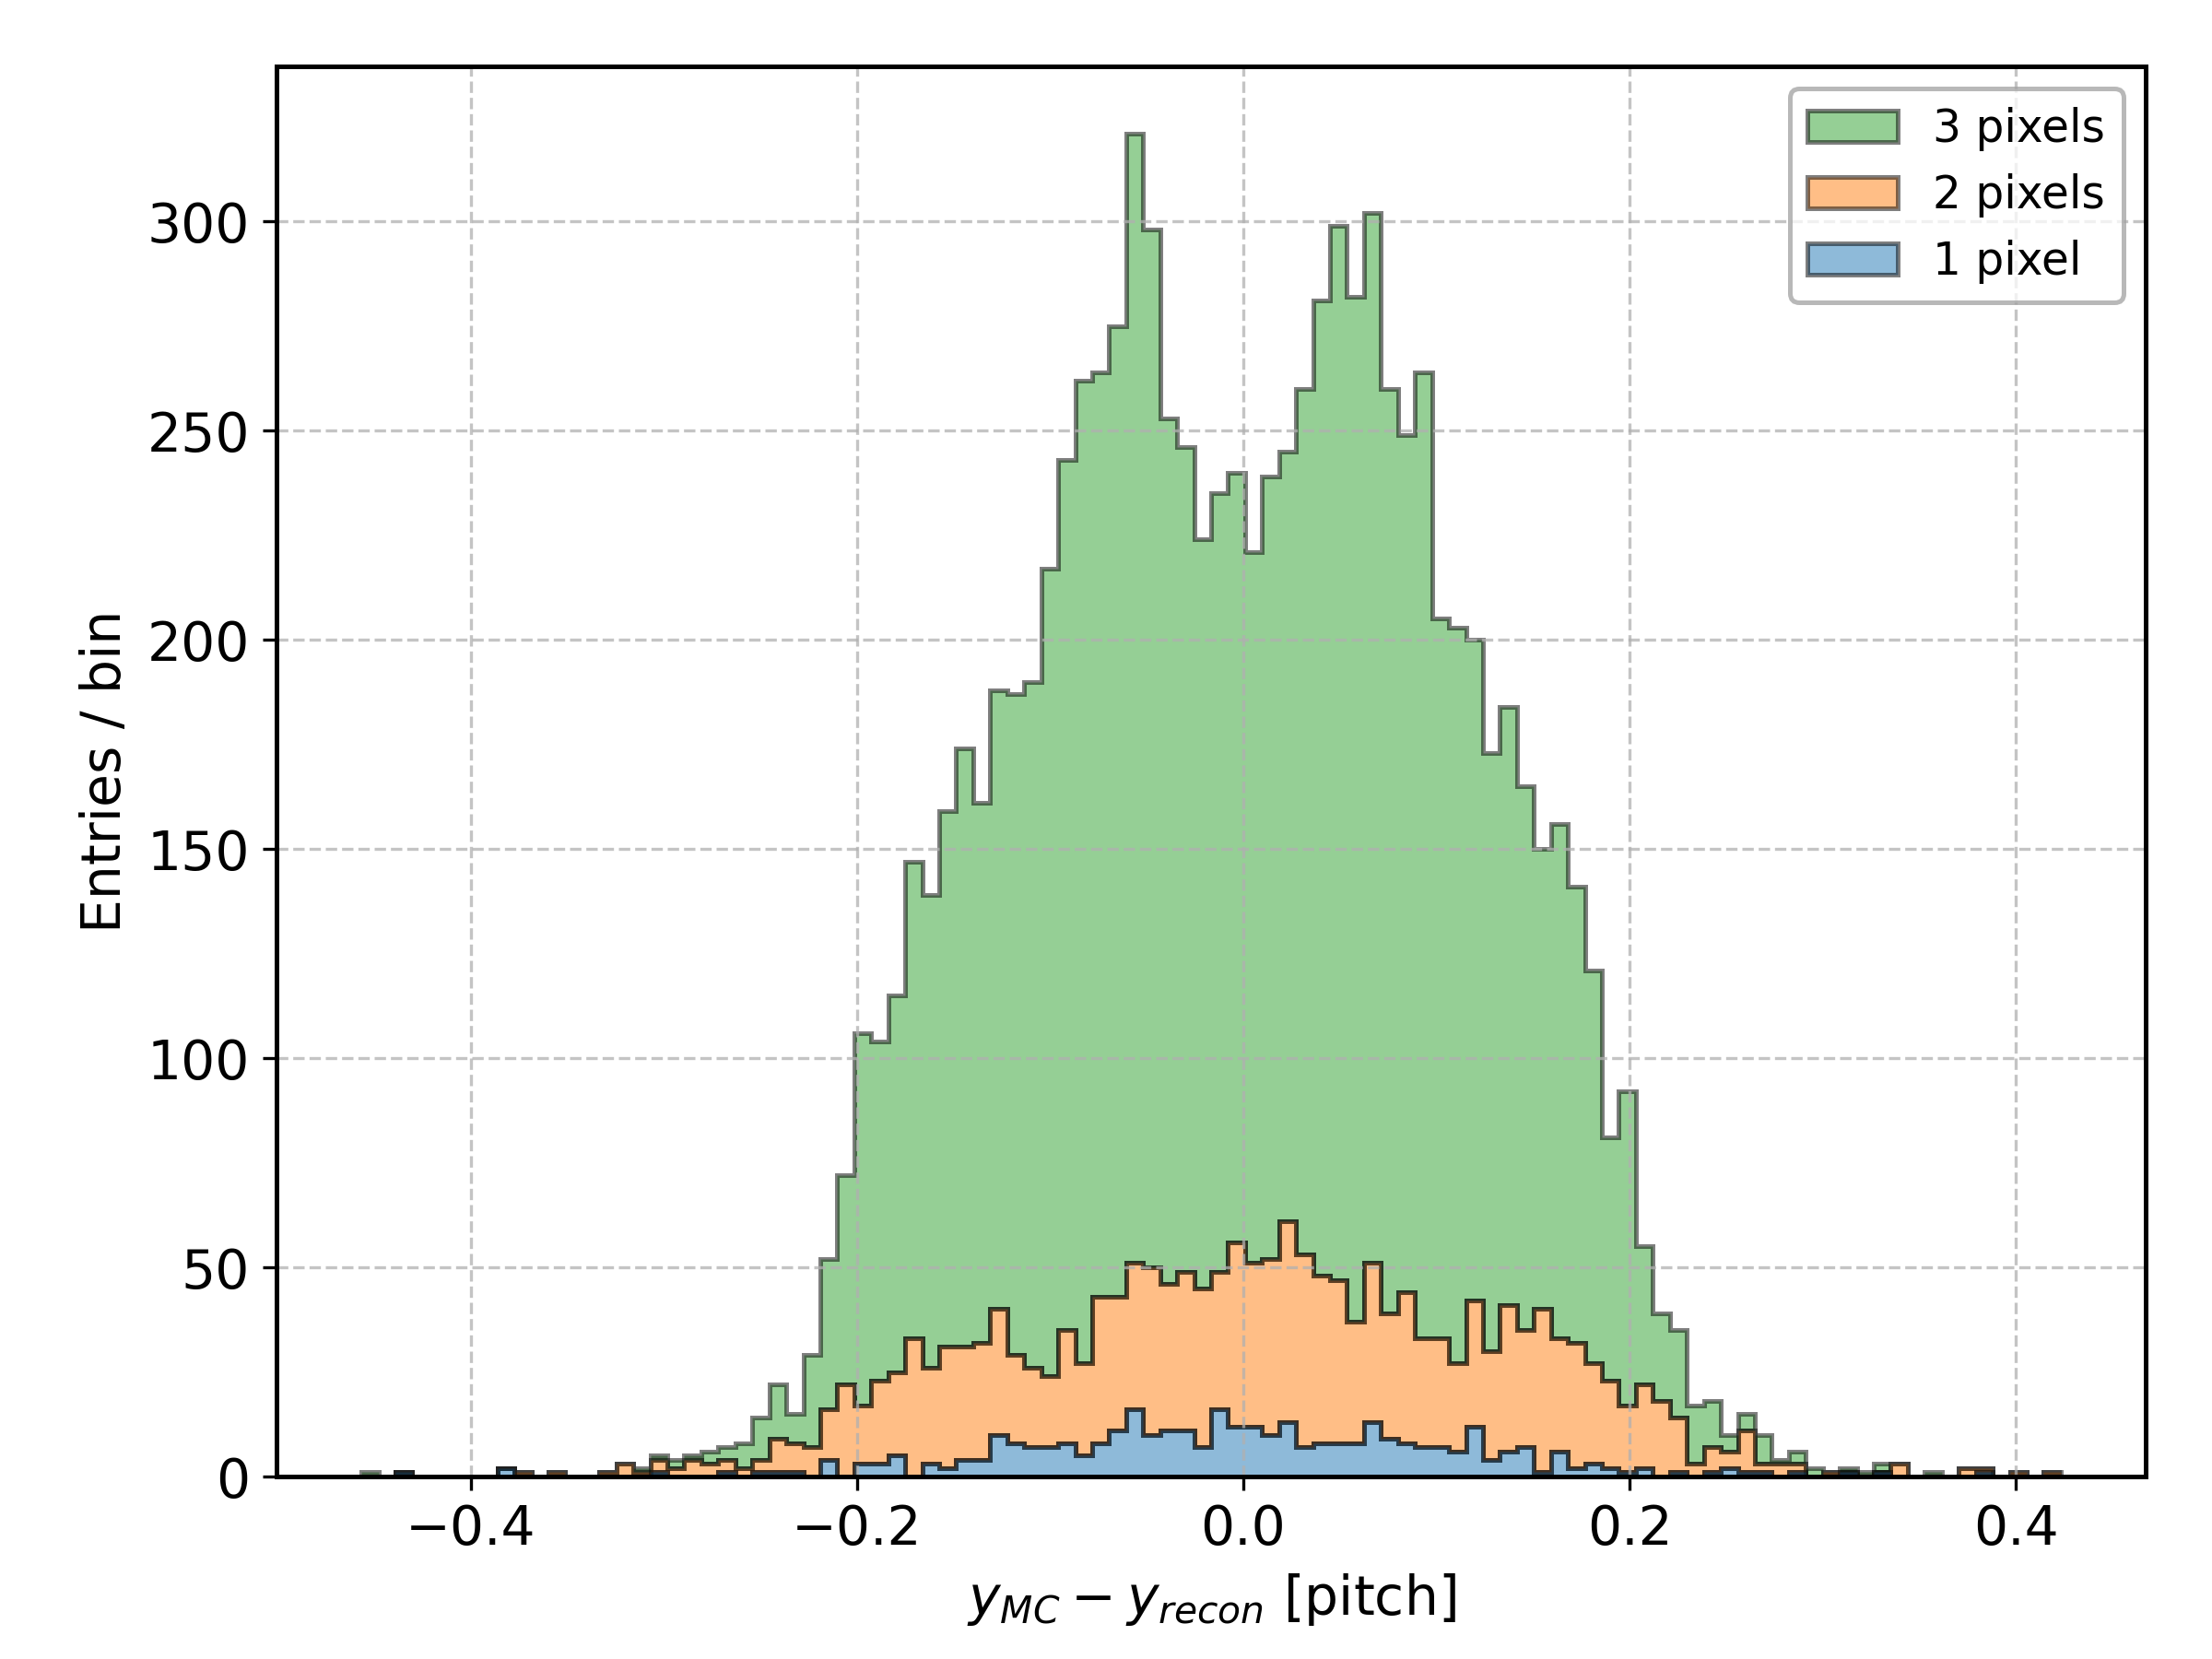
\includegraphics[width=0.49\linewidth]{figures/chapter4/position/barycenter_dy}
    \caption{Residuals distributions for the $x$ and $y$ directions obtained with the charge barycenter algorithm. The residuals are calculated as the difference between the reconstructed and the Monte Carlo truth $x$ and $y$ components. The events are separated by cluster size, with each color representing a specific cluster size. The histograms are stacked on each other. The simulation is made with a 8 keV monochromatic source, 20 ENC of noise and a silicon sensor 300 $\mu$m thick, with a $\langle \sigma \rangle / p = 15$\% .}
    \label{fig:barycenter_dx_dy}
\end{figure}

This method assumes that the charge in each pixel is spread uniformly across it or, equivalently, that it is concentrated in its center. This method does not consider how the charge diffuses inside the active sensor. If the charge would spread on a large number of pixels, this assumption would be valid and the charge barycenter would be a good estimator of the incident position. However, as said above, the detectors are designed to have a small $\langle \sigma \rangle / p$ ratio and the cluster size is small, thus the charge barycenter is not ideal.

It must be noted that for one-pixel events this is the only possible method that can be applied, as there is not enough information to reconstruct a position different from the pixel center. From this point on, it is assumed that every time a one-pixel event is analyzed, the incident position is reconstructed in the pixel center. While these events have the best energy resolution, as will be shown in the next section, they have the worst spatial resolution.

Fig. \ref{fig:barycenter_dx_dy} shows the residuals distributions for the $x$ and $y$ components between the reconstructed and the Monte Carlo truth positions. It is visible how the hexagonal geometry affects the reconstruction, in particular for two-pixels and three-pixels events. The overall distributions are not gaussians and are broad.

By calculating the distance between the truth and the reconstructed positions, the EEF can be calculated. 
Fig. \ref{fig:barycenter_eef} shows how the EEF of the barycenter algorithm varies as a function of the ratio between the diffusion widths of the charge cloud and the pixel pitch. It can be observed that a broader diffusion implies a better resolution. 
%Tab. \ref{tab:eef_barycenter} shows the distance at which EEF contains 50\% and 90\% of the events.

%\begin{table}[htbp]
%\centering
%\begin{tabular}{c cccc}
%$\langle \sigma \rangle / p$ [\%] & EEF@50\% [pitch] & EEF@90\% [pitch]\\
%\midrule
%12.2 & 0.19 & 0.27 \\
%13.7 & 0.17 & 0.24 \\
%15.2 & 0.15 & 0.22 \\
%16.8 & 0.13 & 0.20 \\
%18.3 & 0.11 & 0.18 \\
%\bottomrule
%\end{tabular}
%\caption{Pitch distances at which EEF contains 50\% and 90\% of the events with charge barycenter reconstruction, as a function of the ratio $\langle \sigma \rangle / p$. The values are extracted from Fig. \ref{fig:barycenter_eef}}
%\label{tab:eef_barycenter}
%\end{table}

This algorithm does not require any specific position-calibration models, as it neglects the physical details of charge diffusion. Consequently, it represents a fast, straightforward approach that provides a robust first estimate of the interaction position, relying exclusively on basic noise and gain-corrected pixel data.

\begin{figure}[h]
    \centering
    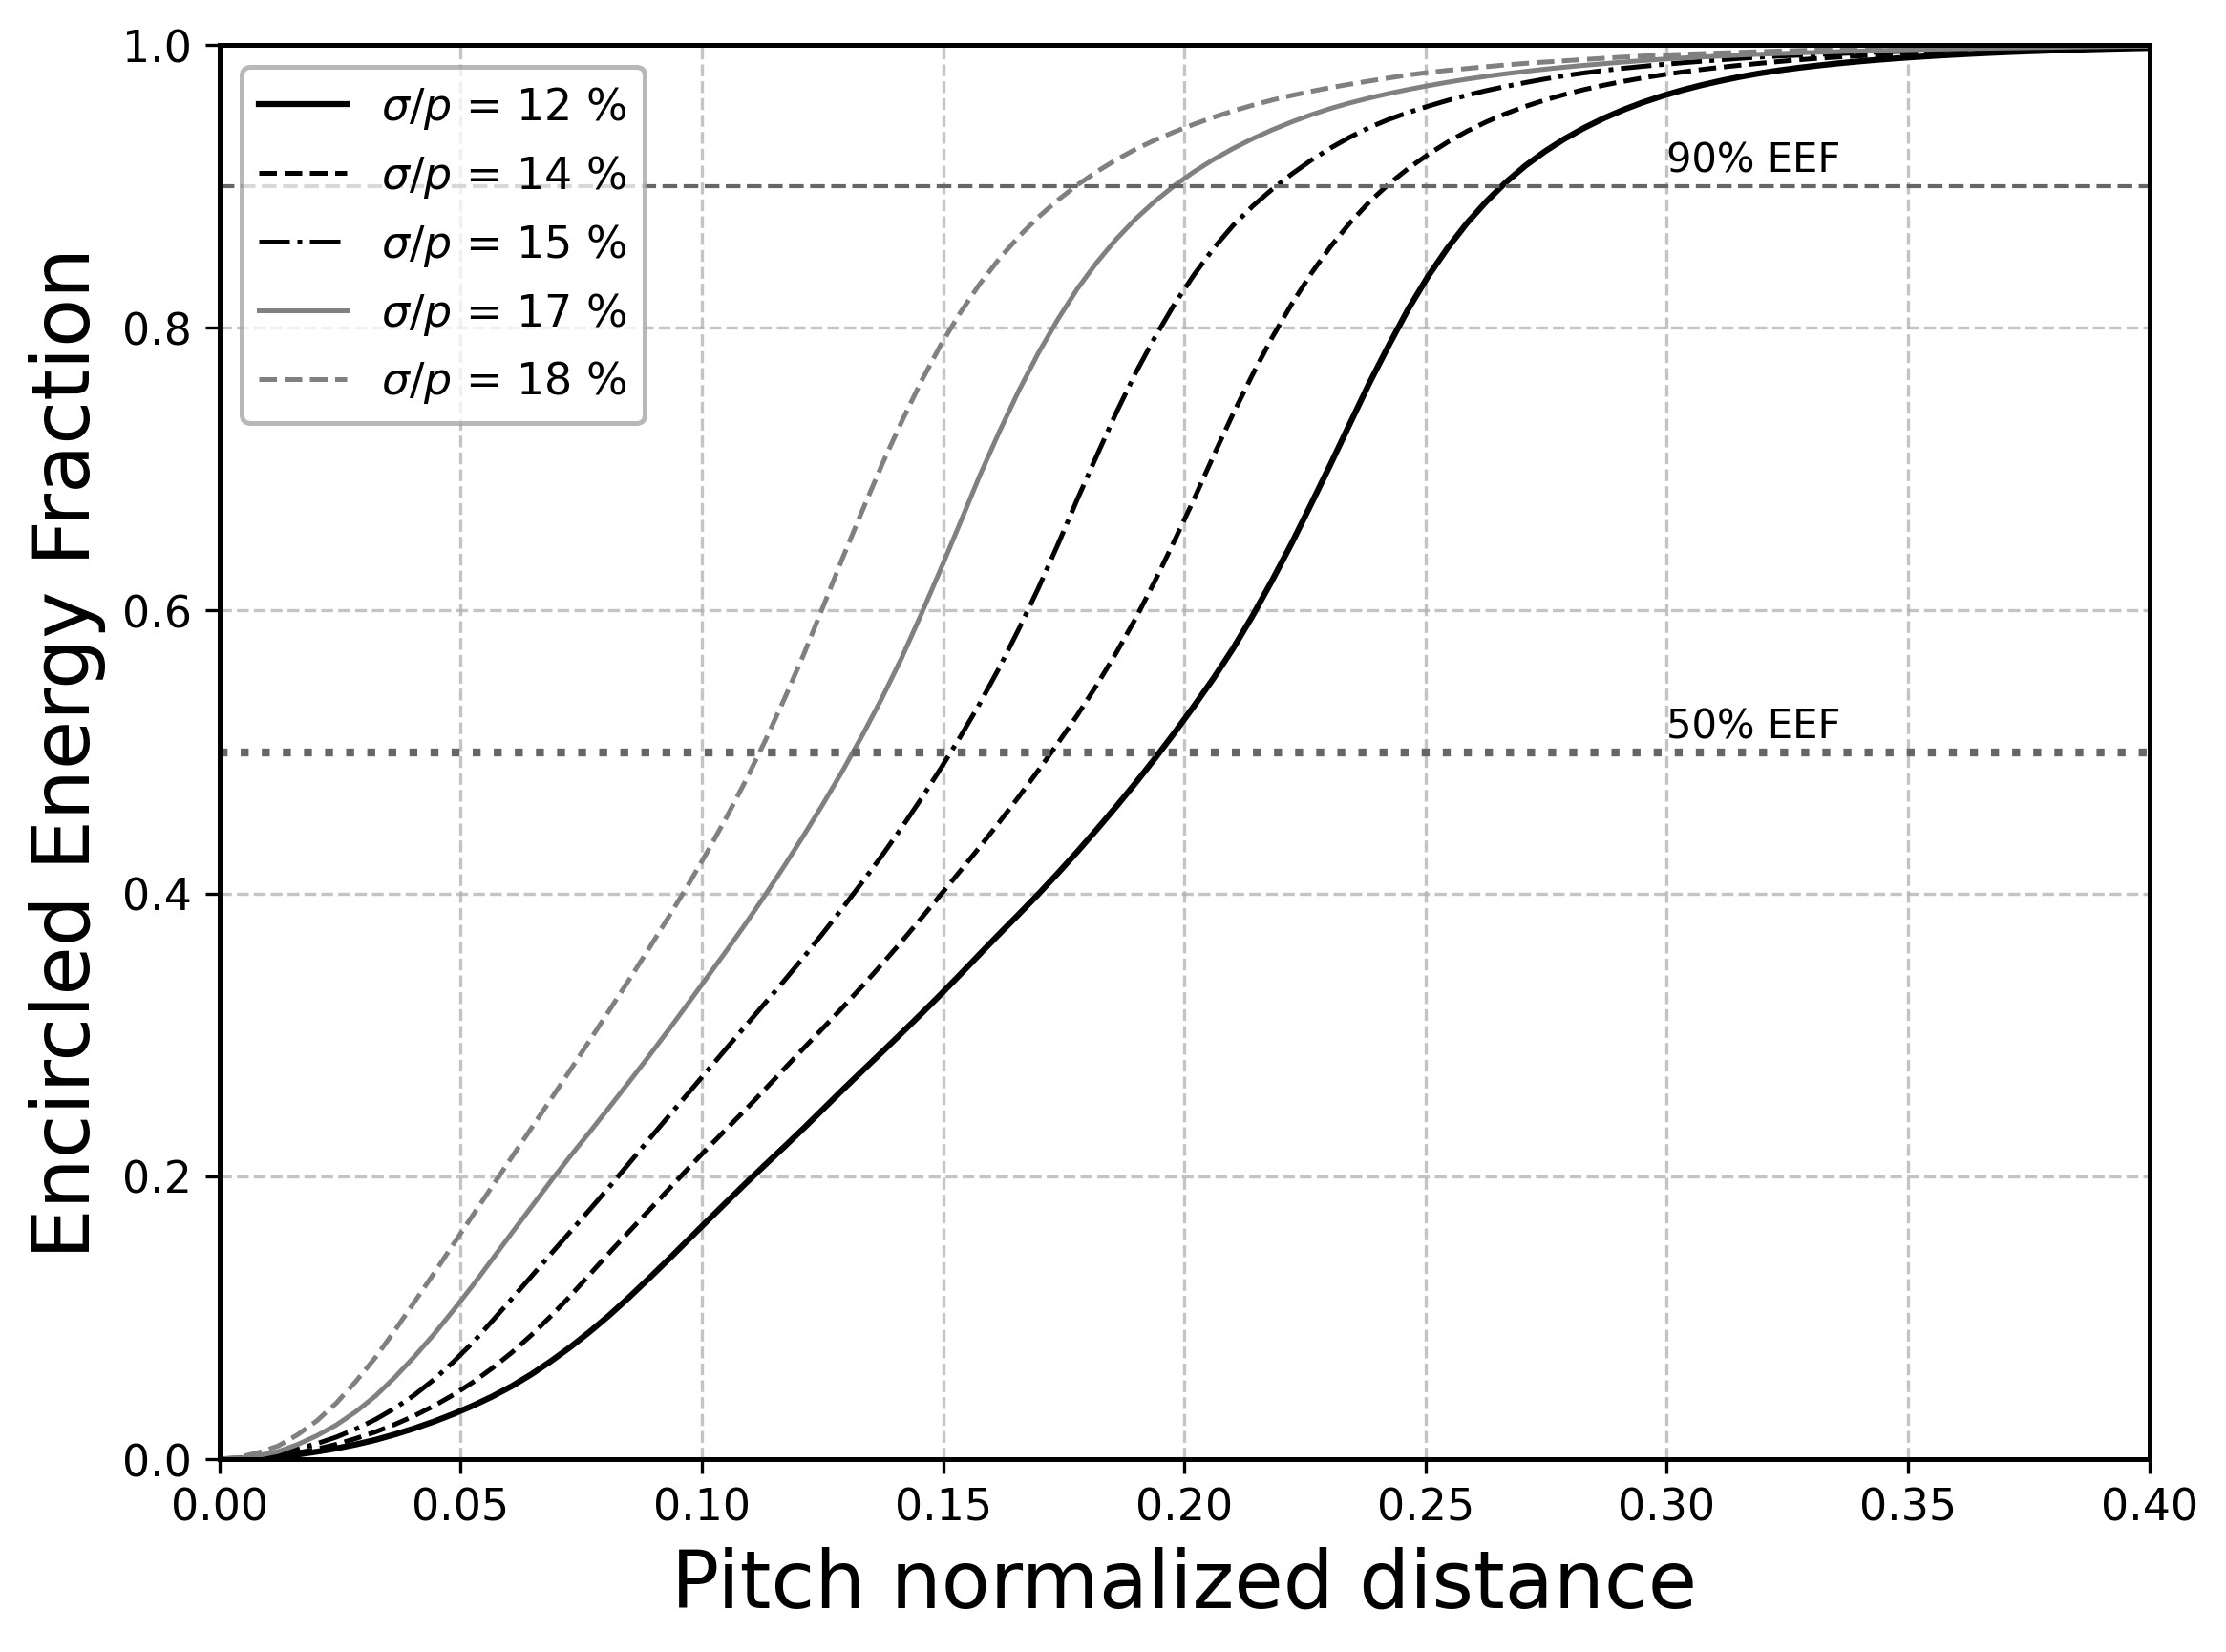
\includegraphics[width=0.7\linewidth]{figures/chapter4/position/barycenter_eef}
    \caption{EEF for different values of the ratio between the diffusion cloud widths and the pixel pitch as a function of the pitch normalized distance. The simulations are made with 20 ENC of noise and a silicon sensor 300 $\mu$m thick. To vary $\langle \sigma \rangle / p$ the diffusion coefficient is varied in the range 40--60 $\mu$m cm$^{-0.5}$.}
    \label{fig:barycenter_eef}
\end{figure}

\subsection{Likelihood estimator}
\label{subsec:mle}

\begin{figure}[!b]
    \centering
    \begin{tikzpicture}[scale=2.5]

    \hexpix{\hexsize}
    \hexpix[xshift=1cm]{\hexsize}
    \hexpix[xshift=-1cm]{\hexsize}
    \hexpix[xshift=0.5cm, yshift=-0.866cm]{\hexsize}
    \hexpix[xshift=-0.5cm, yshift=-0.866cm]{\hexsize}
    \hexpix[xshift=0.5cm, yshift=+0.866cm]{\hexsize}
    \hexpix[xshift=-0.5cm, yshift=+0.866cm]{\hexsize}
    
    \begin{scope}
        \clip (0.3,0.2) circle (0.75cm);
        \fill[shading=paletteScienza, path fading=gaussianaPerfetta, opacity=0.3] (0.3,0.2) circle (0.75cm);
    \end{scope}
    
    \tikzset{
        labelStyle/.style={
            anchor=center, 
            font=\small, 
            text=black, 
            align=center,
            fill=white, 
            fill opacity=0.7, 
            text opacity=1, 
            inner sep=1.5pt, 
            rounded corners=1.5pt
        }
    }

    \node[labelStyle] at (0, -0.15) {$q_0$\\[-2pt]\footnotesize 64.8\%};
    \node[labelStyle] at (1, -0.15) {$q_2$\\[-2pt]\footnotesize 21.5\%};
    \node[labelStyle] at (0.5, 0.866-0.15) {$q_1$\\[-2pt]\footnotesize 10.9\%};
    \node[labelStyle] at (0.5, -0.866-0.15) {$q_3$\\[-2pt]\footnotesize 1.9\%};
    \node[labelStyle] at (-0.5, 0.866-0.15) {$q_6$\\[-2pt]\footnotesize 0.9\%};
    \node[labelStyle] at (-0.5, -0.866-0.15) {$q_4$\\[-2pt]\footnotesize $<0.1\%$};
    \node[labelStyle] at (-1, -0.15) {$q_5$\\[-2pt]\footnotesize $<0.1\%$};

    \fill[black] (0.3, 0.2) circle (0.025cm);
    \node[anchor=south west, font=\scriptsize, text=black, inner sep=1pt] 
        at (0.3, 0.2) {$(x_0, y_0)$};
        
    \end{tikzpicture}
    
    \caption{Example of charge diffusion from a photon with incident position $(x_0, y_0)$ and standard deviation of the bivariate Gaussian equal to 15\% of the pixel pitch. The charge cloud extends up to $5\sigma$, and the calculated charge fractions collected by each pixel ($q_0\text{--}q_6$) are explicitly indicated.}
    \label{fig:mle_model}
\end{figure}

The simple barycenter algorithm totally ignores how the charge diffuses inside the sensor, as it assumes that it uniformly spreads across the involved pixels. As mentioned in Chap. \ref{sec:semiconductors}, the charge diffusion inside the active sensor can be modeled with a bivariate Gaussian distribution centered on the incident position and with a standard deviation $\sigma$ that can be estimated using Eq. \ref{eq:z_average} and the working conditions of the sensor. By normalizing the total charge to 1, the integral of the bivariate distribution over each pixel $P_i$ represents the charge fraction $f_i$ that has been collected by it

\begin{equation}
f_i (x_0, y_0) = \int_{P_i} \frac{1}{2\pi \sigma^2} \exp \left[ - \frac{(x - x_0)^2 + (y - y_0)^2}{2\sigma^2} \right] \,dx\,dy.
\label{eq:mle_charge_fraction}
\end{equation}

The total charge of the event is defined as $Q = \sum_{i=0}^6 q_i$, where $q_i$ is the charge collected by the $i$-th pixel. Assuming that electronic noise is negligible and that charge fluctuations are purely statistical, the joint distribution of charges across the cluster follows a multinomial distribution. From this distribution, the likelihood of the photon incident position $(x, y)$ given the observed charges is defined as:

\begin{equation}
\mathcal{L}(x, y) = \frac{Q!}{\prod_i q_i!} \prod_i f_i(x,y) ^{q_i}.
\label{eq:mle_multinomial}
\end{equation}

If electronic noise is present, the pure multinomial model no longer holds, especially in high-noise conditions, because the observed charge fluctuations become dominated by signal-independent electronic noise rather than charge-partition statistics. 

An example to illustrate this situation is the case of a $8\text{ keV}$ photon absorbed in a silicon sensor, which generates approximately $Q \approx 2200\text{ e}^-$ electron-hole pairs. If the central pixel collects an expected fraction $f_0 = 40\%$ of the total charge, the variance associated with the binomial charge-sharing partition among the pixels is

\begin{equation}
\sigma_{\text{s}}^2 = Q f_0 (1 - f_0) \approx 528.
\end{equation}

For the design goal electronics noise of $\sigma_n = 20\text{ ENC}$, the electronic noise variance is $\sigma_n^2 = 400$. Even for the pixel collecting the largest charge fraction, the statistical partition variance $\sigma_{\text{s}}^2$ and the electronic noise variance $\sigma_n^2$ are of comparable magnitude. For neighboring pixels collecting smaller fractions ($f_i \ll 1$), the partition variance scales as $\sigma_{\text{s}}^2 \approx Q f_i$ and becomes completely overwhelmed by the electronic noise.

To correct this model and adapt it to the presence of electronic noise it is necessary to consider how the noise affects the observations. As seen in Sec. \ref{sec:noise_calibration}, the noise is distributed according to a Gaussian distribution. As a consequence, each pixel charge distribution can be modeled with a Gaussian distribution for the following reasons:

\begin{itemize}[label=-]
\item if a pixel collects many charges, its probability distribution converges to a Gaussian distribution. When the noise is added, the resulting variable is still distributed according to a Gaussian distribution with variance $\sigma^2 = \sigma^2_s + \sigma^2_n$;

\item if a pixel collects a small fraction of charge, its charge distribution follows a binomial distribution with a small probability parameter $f_i$. This distribution is highly asymmetrical, peaked near zero and with a very low variance $\sigma^2_s$, negligible with respect to the electronic noise variance $\sigma^2_n$. This means that when summing the two variables, the noise dominates the signal charge, with the resulting distribution being a Gaussian distribution, whose variance can still be modeled as the sum of the two independent components $\sigma^2 = \sigma^2_s + \sigma^2_n$.
\end{itemize}

Therefore, the charge probability density function of a single pixel is

\begin{equation}
p(q_i; \mu = f_i Q , \sigma^2) = \frac{1}{\sqrt{2\pi}\sigma} \exp \left[- \frac{(q_i - f_i Q)^2}{2\sigma^2} \right],
\label{eq:pdf_mle}
\end{equation}

where $\sigma$ is the standard deviation obtained from the squared sum of the two fluctuation components and $Q$ is the true total charge generated by the photon interaction. It is important to note that, unlike the electronic noise-free scenario, the true charge $Q$ is now an unknown parameter, because the independent electronic noise added to each pixel causes the sum of the measured charges $\sum_i q_i$ to deviate from the true value $Q$.

Eq. \ref{eq:pdf_mle} lacks an important characteristic which is included in Eq. \ref{eq:mle_multinomial}, which is the correlation between the pixels. Indeed, this probability density function does not take into account the fact that if the incident position varies a bit, some pixels lose some of the charge, while others increase it, thus it cannot be assumed that the pixels are independent. To take the pixel correlation into account, a model that takes into account all the pixels at once has to be considered.

To this end, the probability density function is a generic multivariate Gaussian distribution, described by

\begin{equation}
p(\vec{q}; x, y, Q) = \frac{1}{(2 \pi)^{7/2} |V|^{1/2}} \exp{\left[ -\frac{1}{2}(\vec{q} - \vec{f}Q)^{T} V^{-1} (\vec{q} - \vec{f}Q) \right]},
\label{eq:multivariate_gauss}
\end{equation}
where $\vec{q}$ is the seven-dimensional vector with the observed pixels charge, $\vec{f}$ is the vector with the charge fraction values, and $V$ is the covariance matrix, for which the diagonal elements are the squared sums of the multinomial variances and noise fluctuations and off-diagonal elements are the covariances obtained from the multinomial model, which describe the charge sharing mechanism of the cloud

\begin{equation}
V_{ii} = \sigma^2_{s,i} + \sigma^2_{n,i}, \quad \quad V_{ij} = - Q f_i f_j \quad \textrm{for } i \neq j.
\label{eq:cov_matrix}
\end{equation}

For the off-diagonal elements of the covariance matrix the assumption that electronic noise is uncorrelated is made.

In Eqns. \ref{eq:multivariate_gauss} and \ref{eq:cov_matrix}, the dependance from the incident position is hidden inside $\vec{f}$, so both the mean vector and the covariance matrix depend on the unknown parameters $(x, y)$. At this point, the negative log-likelihood can be computed from Eq. \ref{eq:multivariate_gauss} as

\begin{equation}
\operatorname{NLL}(x, y, Q) = -\ln \mathcal{L} = \frac{1}{2}(\vec{q} - \vec{f}Q)^{T} V^{-1} (\vec{q} - \vec{f}Q) +  \frac{1}{2} \ln |V| + \textrm{const.}
\label{eq:nll_multivariate}
\end{equation}

\begin{figure}[!b]
    \centering
    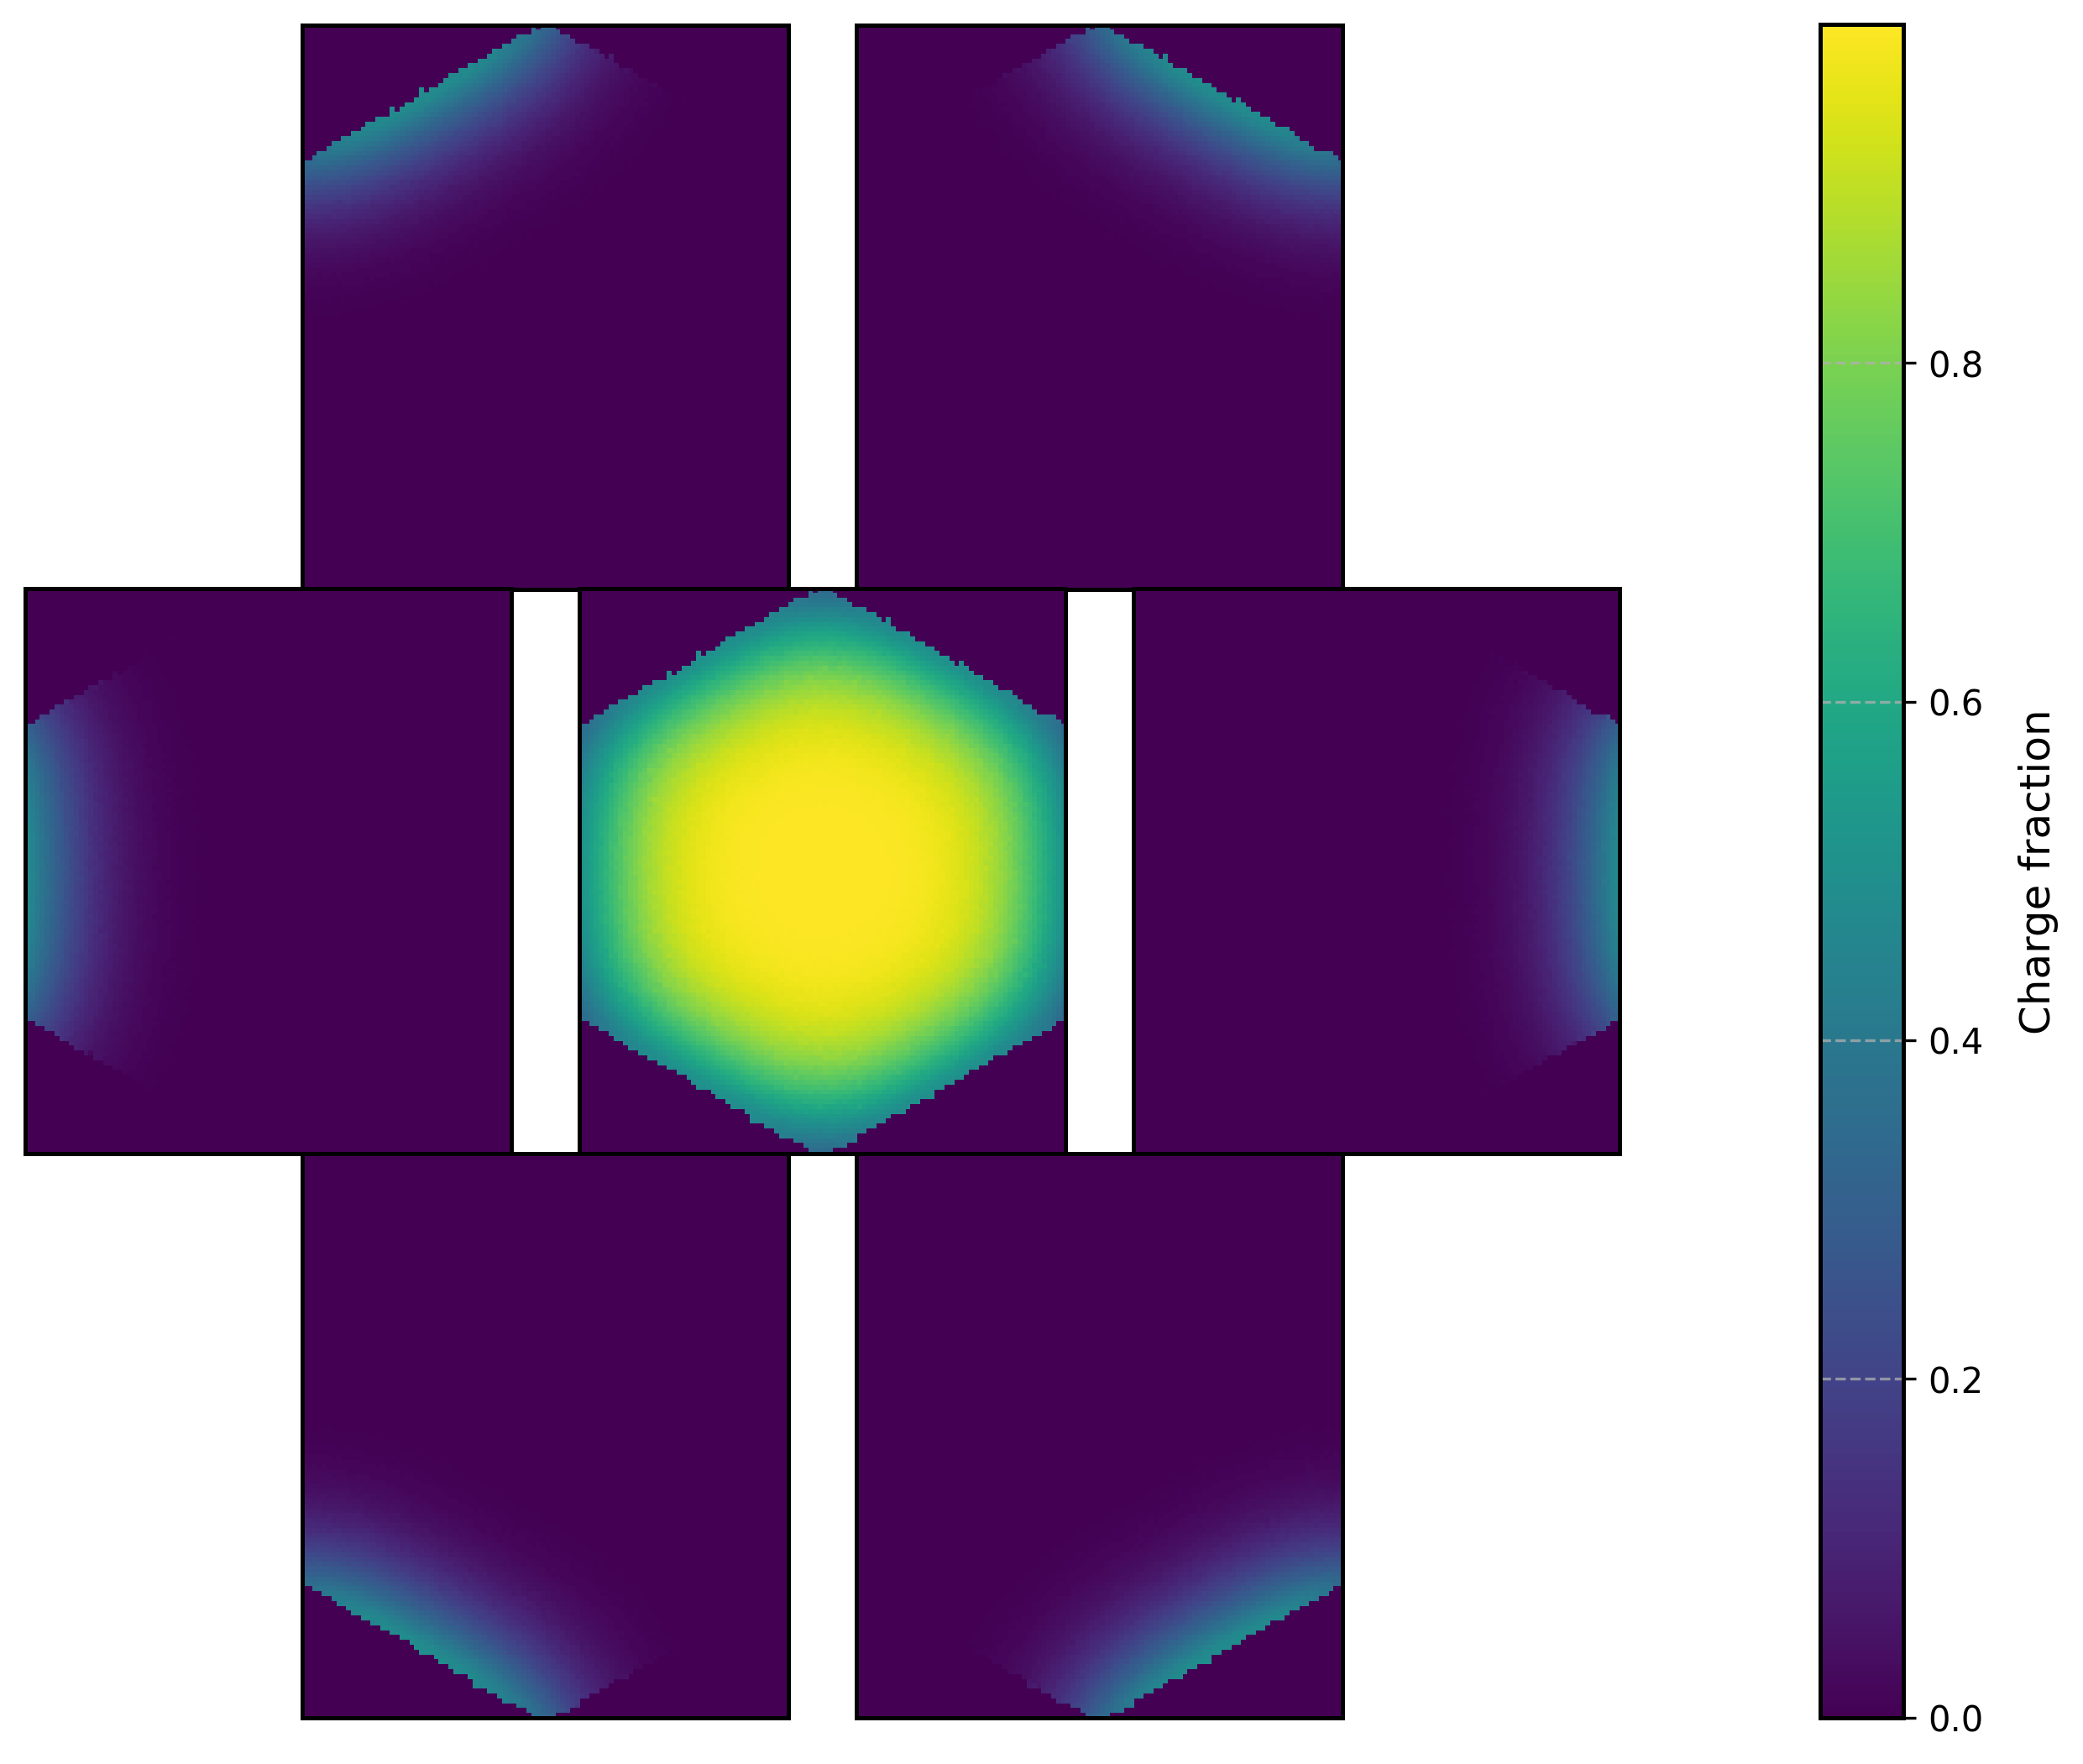
\includegraphics[width=0.48\linewidth]{figures/chapter4/position/calibration_matrices}
    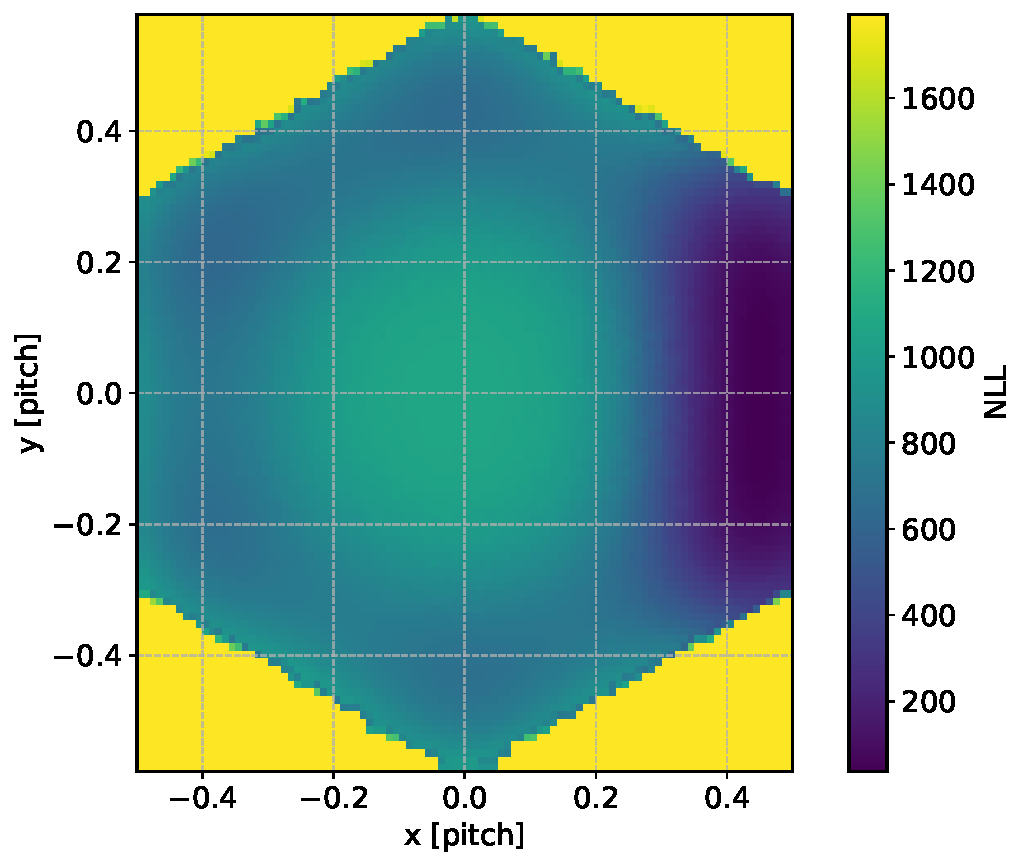
\includegraphics[width=0.48\linewidth]{figures/chapter4/position/nll}
    \caption{Left panel: the seven charge fraction calibration matrices evaluated as a function of the impact position on the central pixel, simulated for a 6 keV monochromatic source with $\langle \sigma \rangle / p \approx 13\%$. The grid is composed of $100 \times 116$ bins. Right panel: two-dimensional map of the $\operatorname{NLL}$ evaluated across the central pixel for a fixed charge $Q$, where the minimum identifies the best-fit reconstructed position $(\hat{x}, \hat{y})$. In the actual fit, $Q$ is free and the minimization is performed in the 3D space $(x, y, Q)$.}
    \label{fig:mle_calibration_and_nll}
\end{figure}

This equation can now be minimized with respect to the unknown parameters $(x, y, Q)$ to find the best-fit incident position and total charge of the event. The minimization is performed with \textit{iminuit} \cite{iminuit}. 

In order to be correctly used, this position reconstruction method requires a prior calibration of the diffusion model. Indeed, the charge fractions depend on the charge cloud diffusion width. The charge fractions $f_i$ could be numerically calculated with Eq. \ref{eq:mle_charge_fraction}, but the hexagonal geometry of the pixels makes the calculation complex. For this reason, the charge-sharing model is evaluated through Monte Carlo simulations and tabulated for a certain value of the $\langle \sigma \rangle / p$ ratio, which is specific to a combination of sensor thickness, pixel pitch, diffusion coefficient and photon energy.

The charge-sharing model calibration is performed using a simulation without noise. A large number of monochromatic events are simulated, then the cluster central pixel is divided into a grid of square bins. For each position bin the average of the charge fraction collected by each of the seven pixels is calculated. The result of the calibration is a set of seven matrices, one for each pixel. Up to a reflection, the matrices of the outer pixels are identical, but for numerical simplicity they are saved and used independently. An example of the set of seven matrices is shown in Fig. \ref{fig:mle_calibration_and_nll}.

During the fit, the minimizer evaluates the $\operatorname{NLL}$ for various values of $(x, y, Q)$. An example of the $\operatorname{NLL}$ evaluated across the pixel for a fixed charge $Q$ is shown in Fig. \ref{fig:mle_calibration_and_nll}. Further details on how the evaluation and minimization of the $\operatorname{NLL}$ are performed are provided in Appendix \ref{appendix:mle}.

\begin{figure}[!b]
    \centering
    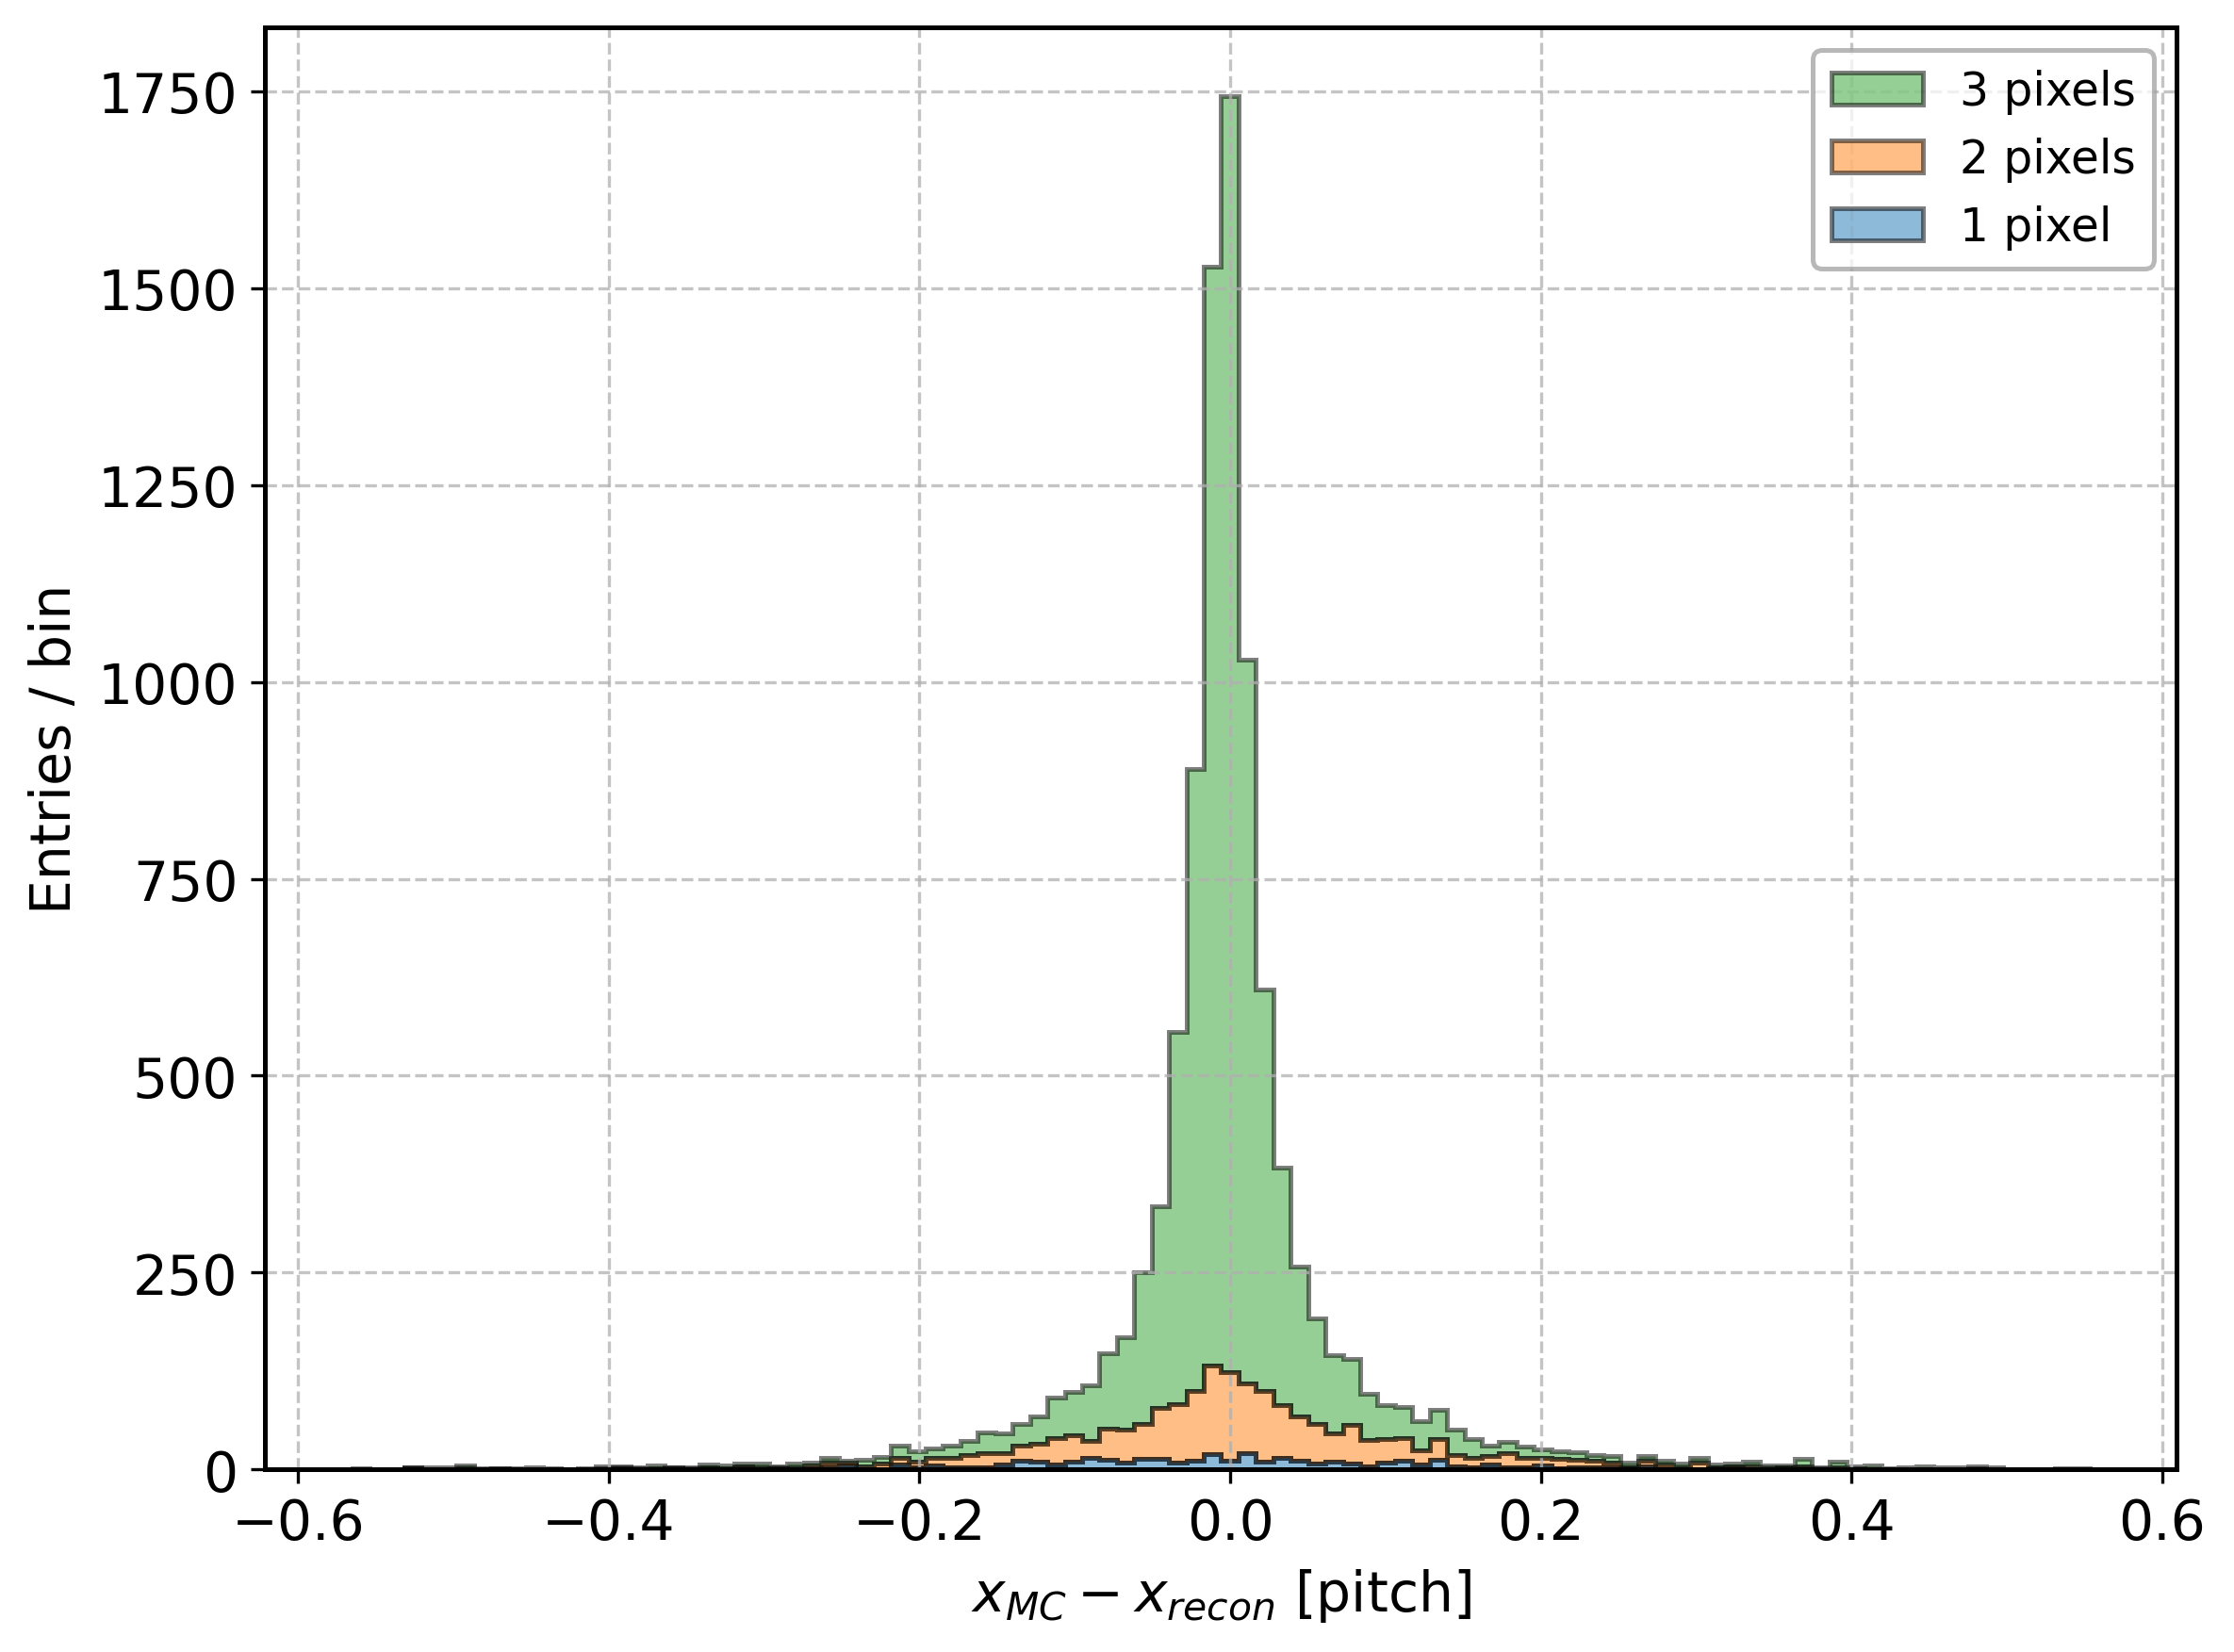
\includegraphics[width=0.49\linewidth]{figures/chapter4/position/mle_dx}
    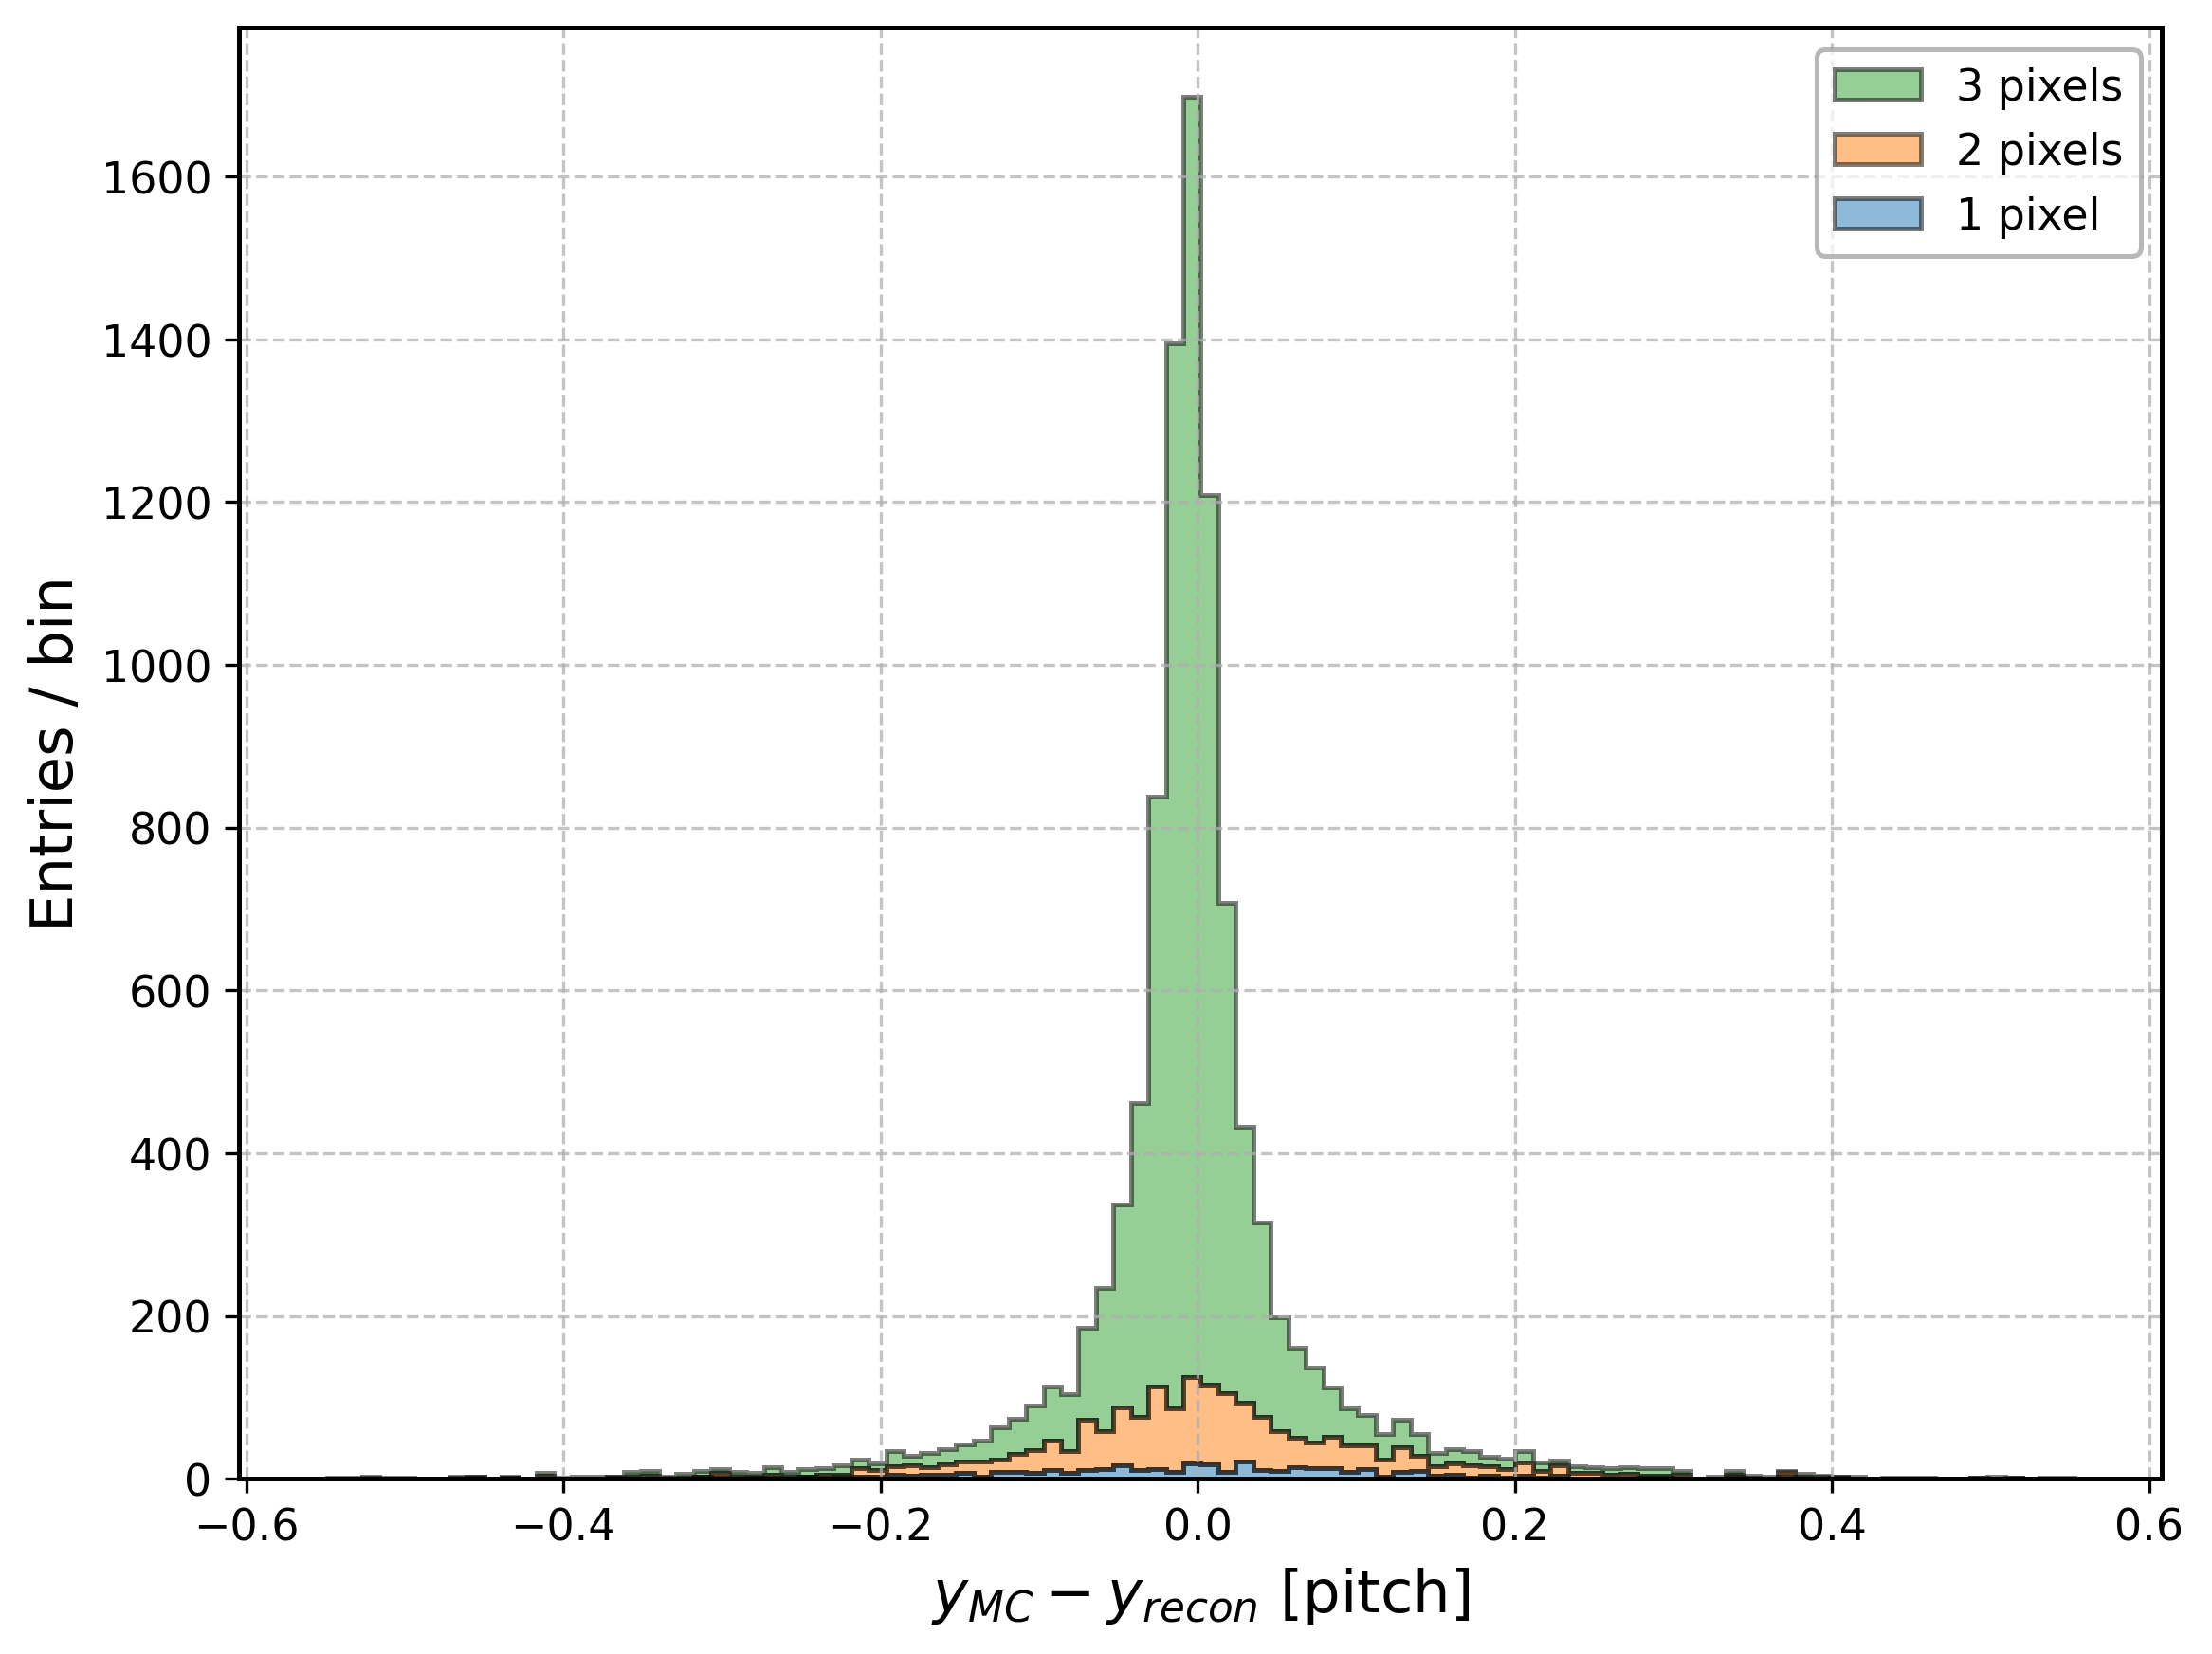
\includegraphics[width=0.49\linewidth]{figures/chapter4/position/mle_dy}
    \caption{Residuals distributions of the maximum likelihood reconstruction algorithm for the $x$ and $y$ directions, calculated as the difference between the reconstructed and the Monte Carlo truth $x$ and $y$ components. The events are separated by cluster size, with each color representing a specific cluster size. The histograms are stacked on each other. Cluster sizes are obtained from the reconstruction described in Sec. \ref{subsec:barycenter}. The simulation is made with a 8 keV monochromatic source, 20 ENC of noise and ratio between the diffused charge cloud sigma and the pitch of 15\%.}
    \label{fig:mle_dx_dy}
\end{figure}

Contrary to charge barycenter, this algorithm does not implement any type of suppression. Indeed, while charge barycenter applies a zero-suppression threshold and a position-suppression to suppress pixels that have high probability of having only noise signal, this algorithm weights each pixel by considering their charge and the calibrated diffusion model. As a consequence, defining the cluster size becomes ambiguous. For plotting purposes and to compare different algorithms, the cluster size used in Fig. \ref{fig:mle_dx_dy} to separate events is the cluster size that is obtained with the charge barycenter algorithm. Fig. \ref{fig:mle_dx_dy} shows the residuals distributions for the $x$ and $y$ position components. With this algorithm the residuals distributions are regular and unimodal. Moreover, the width of the distribution is much smaller than the previous algorithm. 

The only problem arises in the tails of the distributions, that show some residuals up to $\pm 0.6$ times the pixel pitch. This behaviour is well visible in Fig. \ref{fig:mle_eef}, where it is possible to see that the EEF has very long tails, particularly for small diffusion widths. This algorithm is generally better than the charge barycentering, indeed the EEF@50\% is always about three times smaller, but due to the long tails the EEF@90\% can be worse in some cases. 
%Tab. \ref{tab:eef_mle} shows exactly this feature because while the EEF@50\% is about three times smaller than the charge barycenter, the EEF@90\% can be worse in particular cases. 

Furthermore, the same dependence on the diffusion width as the charge barycenter can be observed, with broader diffusions that have a better spatial resolution. It must be noted that for the position reconstruction a set of calibration matrices has been produced for each diffusion width.

\begin{figure}[h]
    \centering
    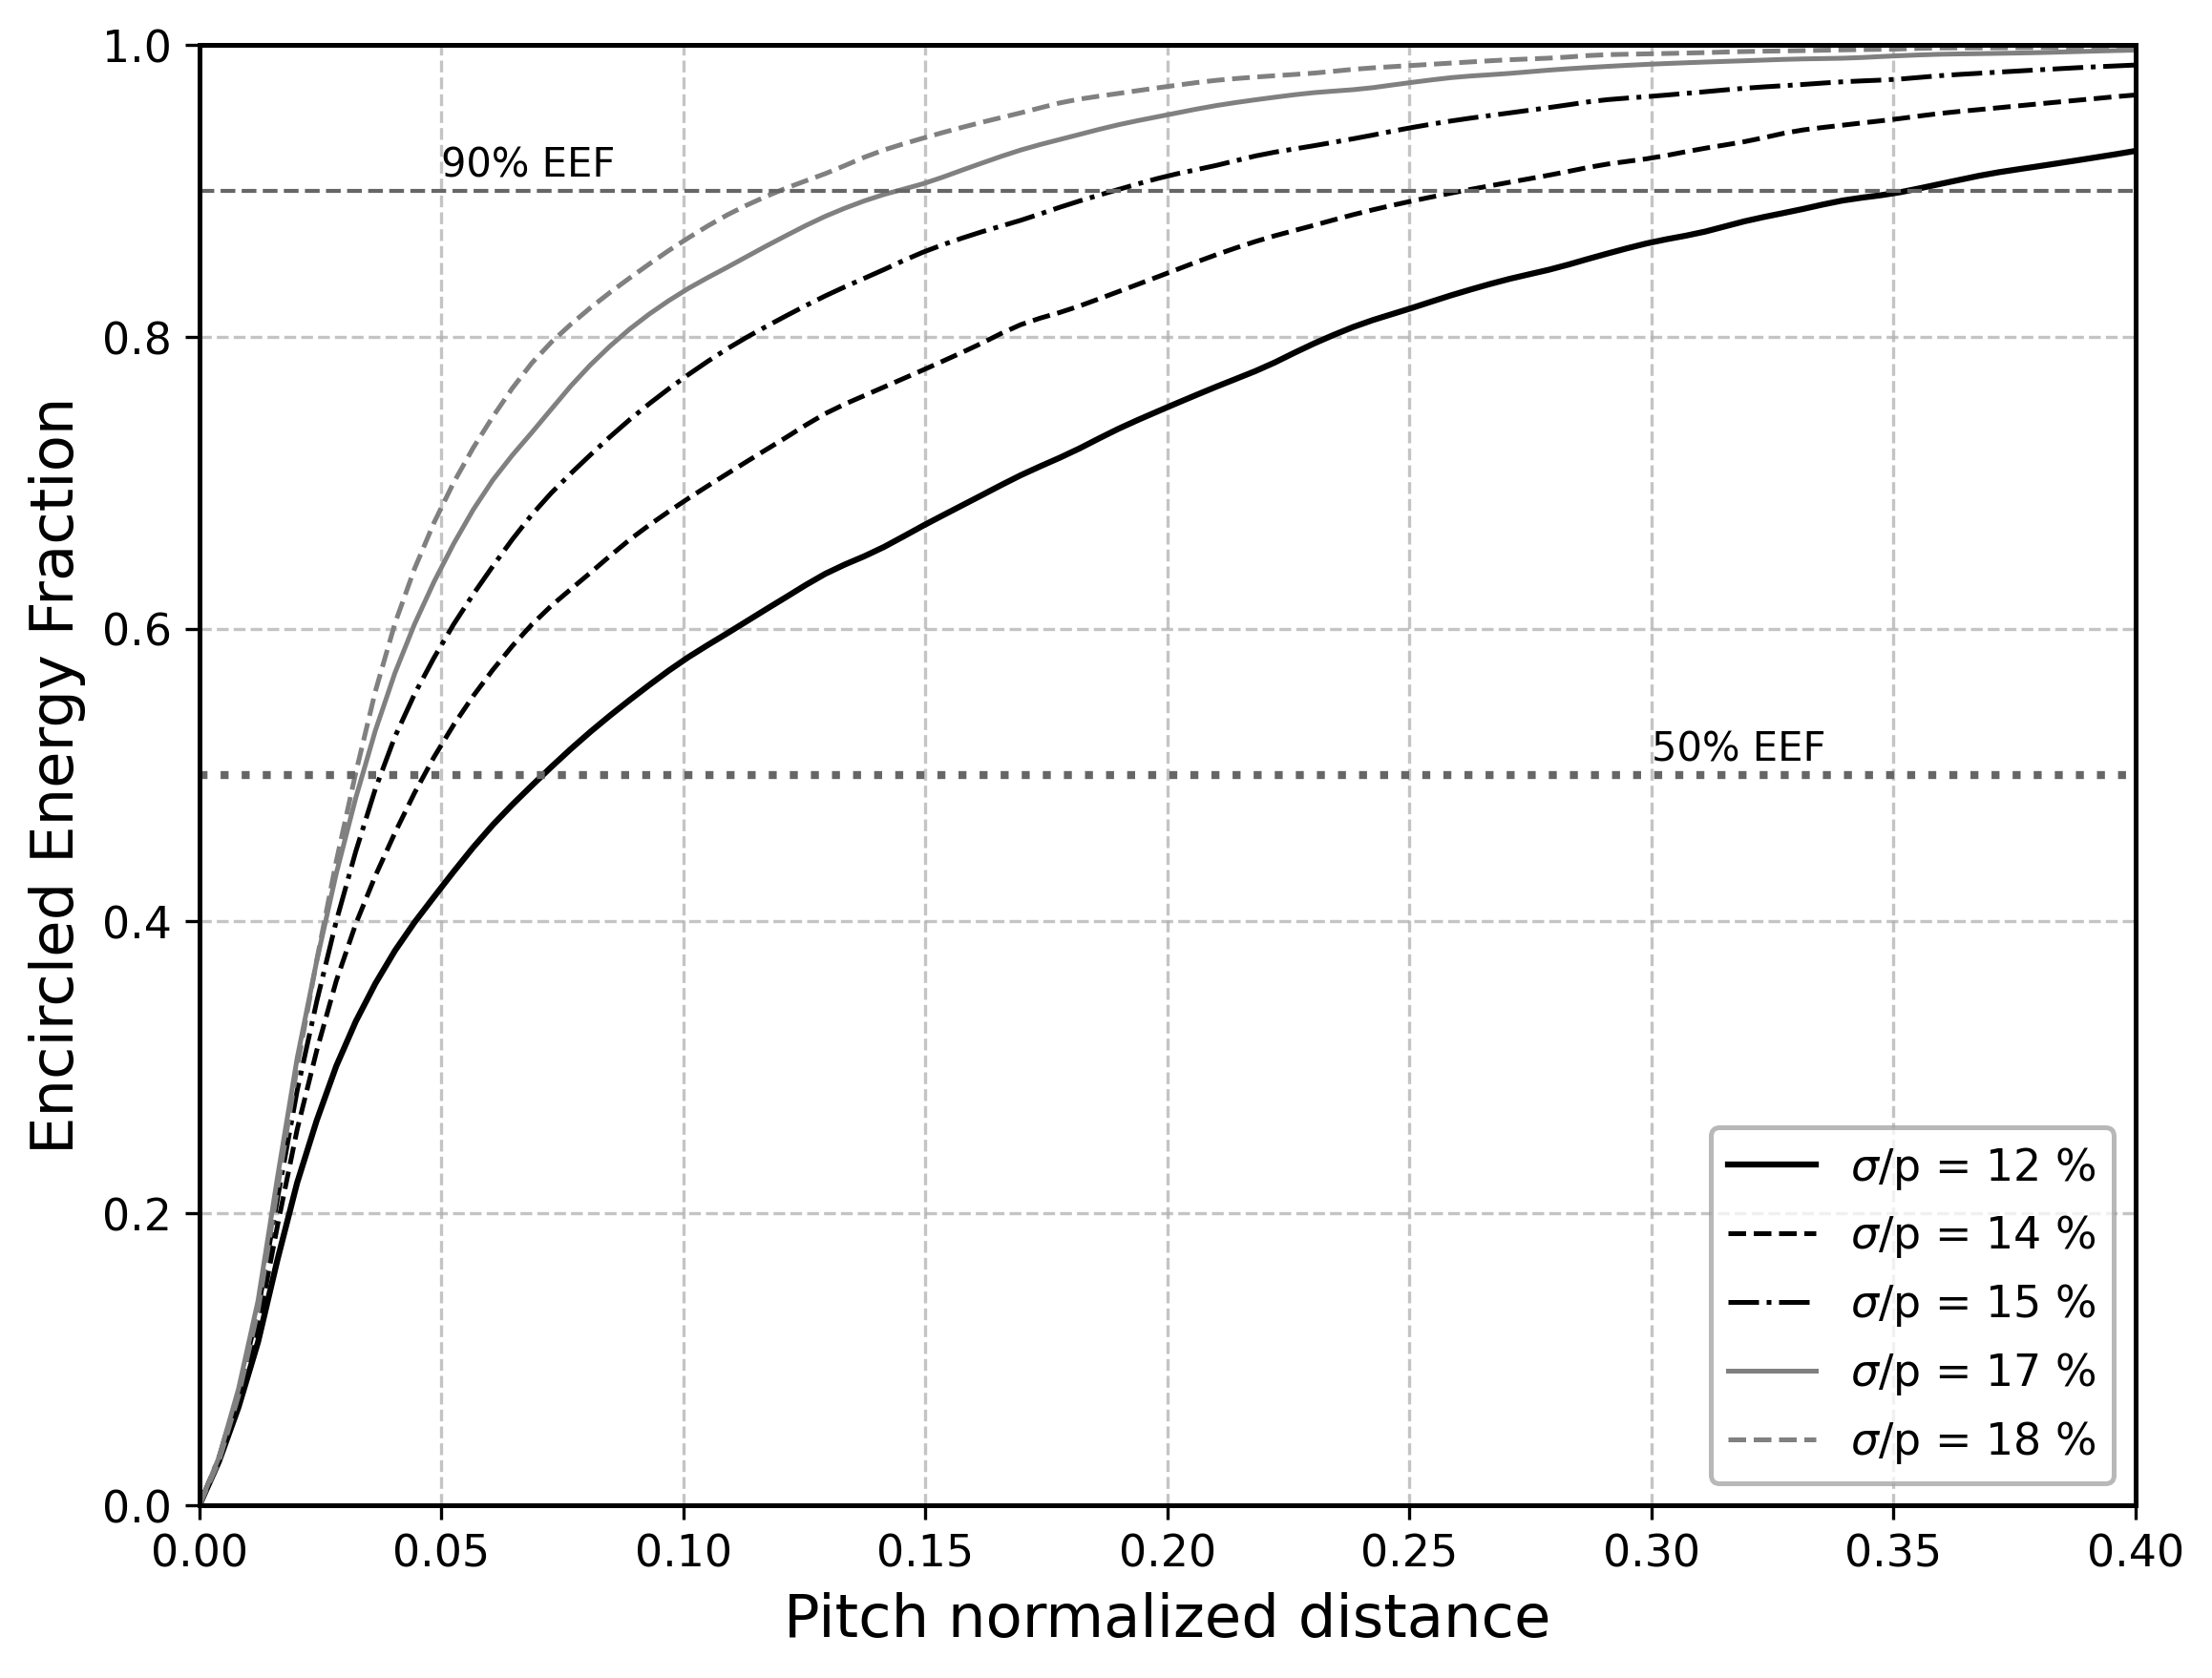
\includegraphics[width=0.7\linewidth]{figures/chapter4/position/mle_eef}
    \caption{Encircled energy fraction of the maximum likelihood estimator reconstruction for different values of the ratio between the diffused charge cloud and the pixel pitch as a function of the pitch normalized distance. The simulation is made with 20 ENC of noise.}
    \label{fig:mle_eef}
\end{figure}

%\begin{table}[htbp]
%\centering
%\begin{tabular}{c cccc}
%$\langle \sigma \rangle / p$ & EEF@50\% [pitch] & EEF@90\% [pitch]\\
%\midrule
%12.2 & 0.07 & 0.35 \\
%13.7 & 0.05 & 0.26 \\
%15.2 & 0.04 & 0.19 \\
%16.8 & 0.03 & 0.14 \\
%18.3 & 0.03 & 0.12 \\
%\bottomrule
%\end{tabular}
%\caption{Pitch distances at which EEF contains 50\% and 90\% of the events with maximum likelihood estimator reconstruction, as a function of the ratio $\langle \sigma \rangle / p$. The values are extracted from Fig. \ref{fig:mle_eef}}
%\label{tab:eef_mle}
%\end{table}


\subsection{$\eta$ algorithm}
\label{subsec:eta}
In the context of silicon microstrip detectors, a common and widely used algorithm to reconstruct the incident position of radiation is the so-called $\eta$ algorithm \cite{belau1983, turchetta1993}. This algorithm, in the case when only two strips have collected signal, is based on the definition of the $\eta$ variable

\begin{equation}
\eta = \frac{q_R}{q_L + q_R},
\label{eq:def_eta}
\end{equation}
that for a microstrip detector is the ratio between the charge $q_R$ collected by the right strip and the total charge collected by the two strips (right and left) involved in the event. By characterizing the distribution of this variable and studying the relation with the incident position, it is possible to obtain a non-linear algorithm, that contrary to the charge barycenter takes into account how the charge diffuses, like the maximum likelihood estimator algorithm.

Assuming that the events are uniformly distributed between the two strips, the typical distribution of $\eta$ is a U-shaped curve, peaked near $\eta = 0$ and $\eta = 1$ and symmetrical with respect to $\eta = 0.5$. The cumulative distribution of $\eta$ gives the relation between the distance from the left strip  of the impact point of the radiation and the observed value of $\eta$. The two distributions are shown in Fig. \ref{fig:belau_eta}.

\begin{figure}
    \centering
    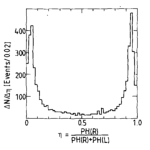
\includegraphics[width=0.45\linewidth]{figures/chapter4/position/belau_eta}
    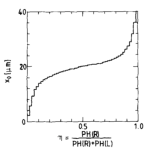
\includegraphics[width=0.45\linewidth]{figures/chapter4/position/belau_cumulative}
    \caption{In the left panel, experimental distribution of the $\eta$ variable calculated for a silicon microstrip detector. In the rigth panel, the cumulative distribution calculated from the latter, which gives the calibration function to reconstruct the event incident position. Images taken from \cite{belau1983}.}
    \label{fig:belau_eta}
\end{figure}

This methodology can also be generalized to the case of hexagonal pixel detectors, but there are some things that need to be modified. The main difference is the two-dimensional nature of position reconstruction on hexagonal pixels. For this reason, the discussion has to be separated depending on the cluster size. The second difference is that, contrary to microstrips, projecting the events belonging to a specific cluster size onto the chosen reconstruction axis does not yield a uniform one-dimensional distribution. Even under a perfectly uniform 2D illumination of the sensor, this projection is inherently non-uniform due to the hexagonal geometry of the pixels. Given that the uniform event distribution is a fundamental requirement to use this method, as stated in \cite{belau1983}, it is necessary to apply geometrical corrections which depend on the pixel shape and on the event typology.

These corrections can be calculated from a Monte Carlo simulation with a source that illuminates the detector with a uniform beam. Using Monte Carlo truth positions, the event distribution along the relevant axis for the event typology can be calculated. These distributions can be used to correctly weight the $\eta$ distributions as if the events were uniformly distributed along the axis. The approach that has been used for each event typology will be explained in the following paragraphs.

As said for the charge barycenter algorithm, for one-pixel events there is nothing that can be done, thus the reconstructed position must coincide with the pixel center.

\begin{figure}[!t]
    \centering
    \begin{tikzpicture}[scale=4]
    \hexpix{\hexsize}
    \node[anchor=south] at (0, 0) {$q_0$};
    \begin{scope}
        \clip (0,0) -- (30:\hexsize) -- (-30:\hexsize) -- cycle;
        \fill[pattern=north east lines, pattern color=gray] (-1,-1) rectangle (1,1);
    \end{scope}
    \hexpix[xshift=1cm]{\hexsize}
    \node[anchor=south] at (1, 0) {$q_1$};
    \draw[|-|] (0, 0.75) -- (1, 0.75);
    \node[anchor=south] at (0.5, 0.75) {$p$};
    \draw[->] (0, 0) -- (1.75, 0);
    \node[anchor=west] at (1.75, 0) {$r$};
    \end{tikzpicture}
    \caption{Illustration of the two-pixel event topology. Assuming that  $q_1 \leq q_0$, 
    the hatched triangle represents the portion of the phase space in terms of the 
    true impact point originating this topology. The $r$ axis is where the event position is reconstructed.}
    \label{fig:two_pixel_event}
\end{figure}

The case of two-pixel events is more interesting, and it can be treated in a similar way as a microstrip detector. Considering the readout design of ASIX, where the triggering pixel is always located at the center of a seven pixel cluster, a small change in the definition of $\eta$ is necessary, which is now defined as
\begin{equation}
\eta = \frac{q_1}{q_0 + q_1},
\label{eq:eta_2pix}
\end{equation}
where $q_0$ is always the central pixel of the cluster and $q_1$ is one of the outer pixels. This means that for ASIX the definition of left and right has no more sense as in microstrips detector. This change in the definition affects the shape of the $\eta$ variable distribution, because now it ranges in the interval $(0, 0.5)$ and does not have a double peak as in Fig. \ref{fig:belau_eta}. 

Before calculating the $\eta$ distribution it is necessary to verify if two-pixel events are uniformly distributed along the axis that connects the two pixel centers shown in Fig. \ref{fig:two_pixel_event}. The scatter plot shown in Fig. \ref{fig:2pix_scatter} shows how the real impact position of two-pixel events are distributed. By observing the count distribution of these events projected onto the axes connecting the center of the central pixel with the outer ones, shown in Fig. \ref{fig:2pix_scatter} as well, it is possible to see that the events are not uniformly distributed.

\begin{figure}
    \centering
    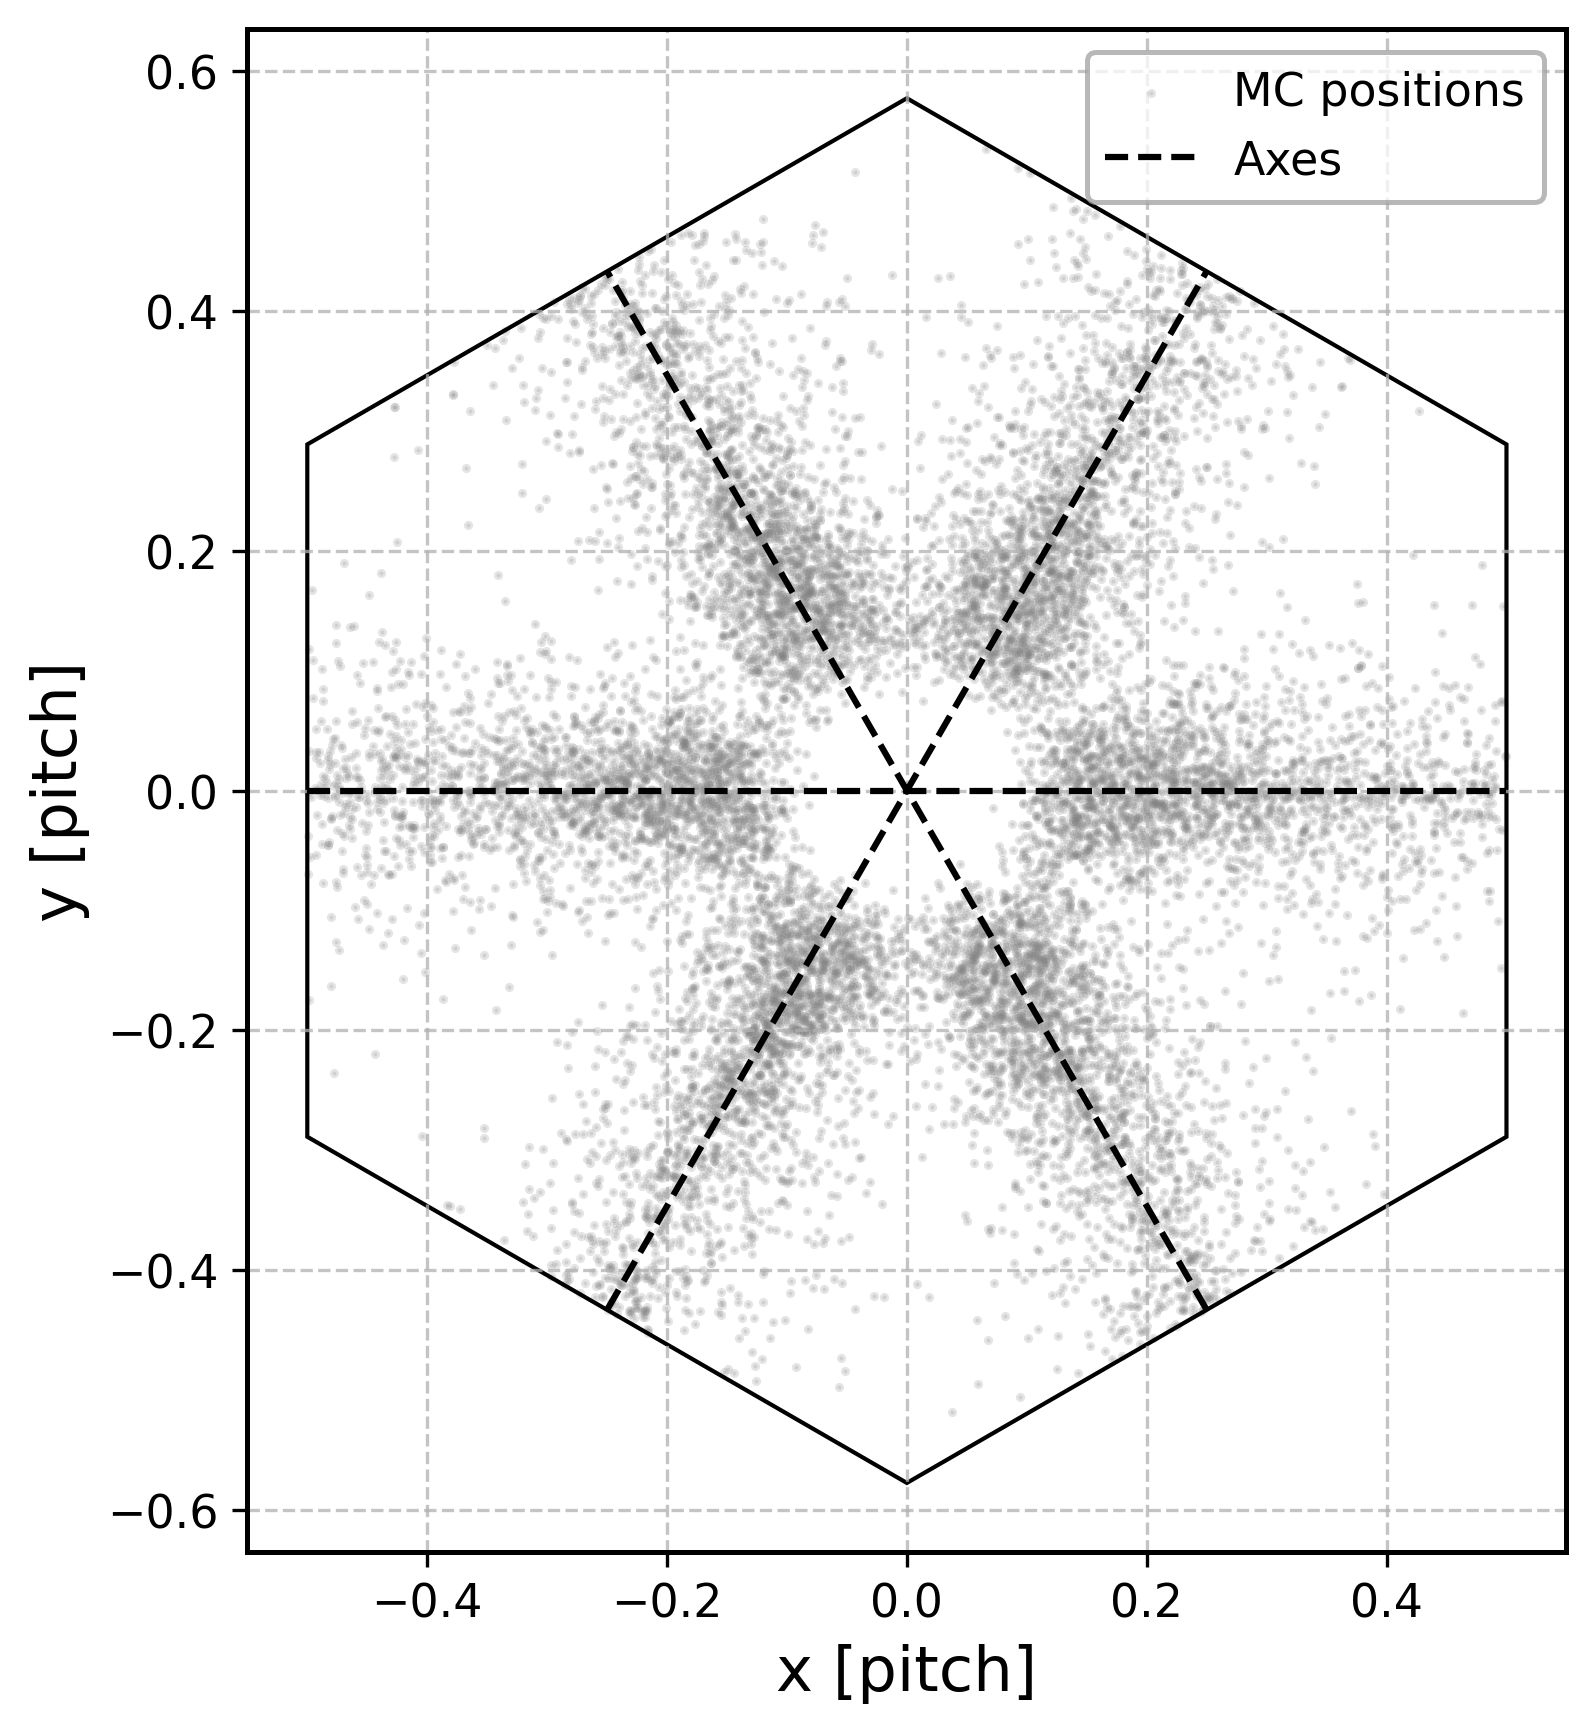
\includegraphics[width=0.35\linewidth]{figures/chapter4/position/eta_2pix_scatter}
    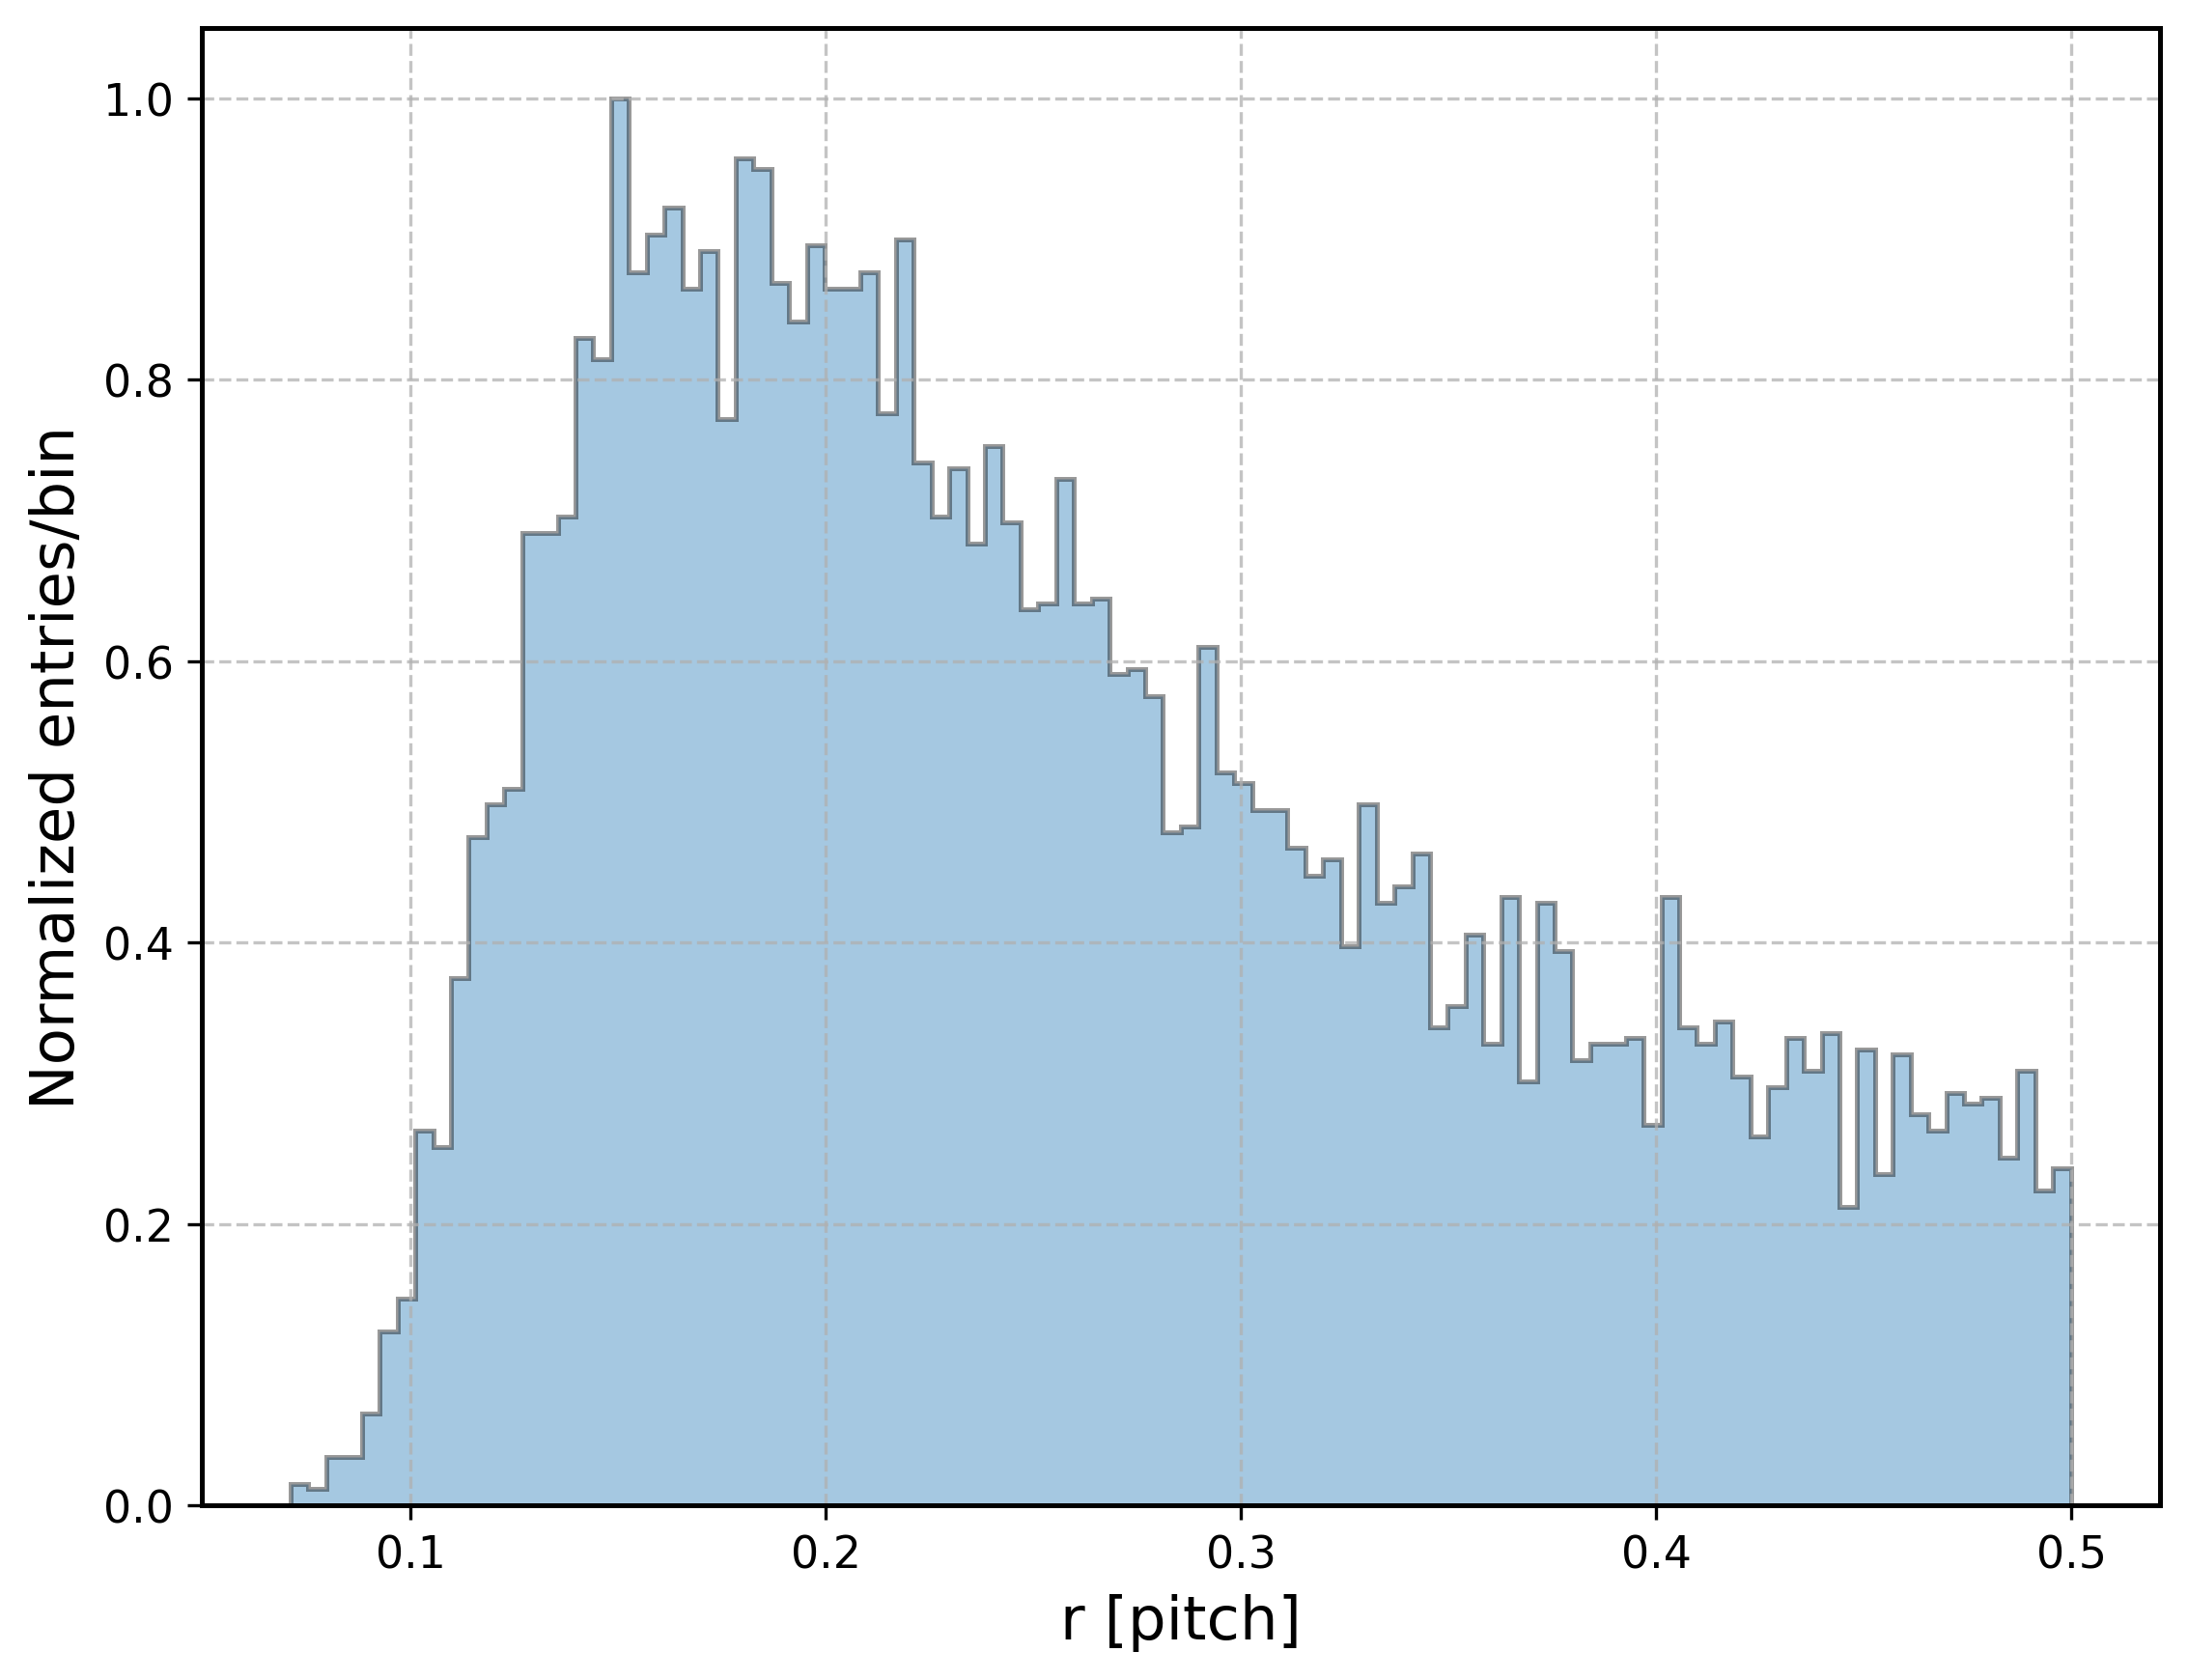
\includegraphics[width=0.49\linewidth]{figures/chapter4/position/eta_2pix_dr_hist}
    \caption{Scatter plot of Monte Carlo truth impact positions of two-pixel events on the central pixel (left panel) and event count distribution of the events projected onto the relevant axes, shown with dashed lines (right panel).}
    \label{fig:2pix_scatter}
\end{figure}
%
%To apply the geometrical correction to the $\eta$ distribution, an iterative procedure is adopted. In the initial step, the relationship between $\eta$ and the position $r$ is assumed to be linear, mapping the minimum and maximum observed values of $\eta$ to the boundaries of the $r$ interval. Using this preliminary $r(\eta)$ mapping, the $\eta$ distribution is corrected by weighting the counts in each $\eta$ bin by the inverse of the spatial density at the corresponding position $r$. The cumulative distribution function of this weighted $\eta$ histogram is then calculated, yielding an updated, non-linear calibration function $r(\eta)$. This new mapping is fed back into the previous step to re-evaluate the weights for the next iteration. The process is repeated until the relation $r(\eta)$ converges to a stable shape. The resulting distributions are shown in Fig. \ref{fig:eta_2pix}. For the final event reconstruction, the cumulative distribution is interpolated to obtain a continuous function $r(\eta)$.
%

To apply the geometrical correction on the $\eta$ distribution, an iterative approach can be adopted. Calling $g(\eta)$ the measured $\eta$ distribution and $\rho(r)$ the event spatial distribution along the reconstruction axis $r$. In the first step $n=0$, the relation between $\eta$ and $r$ is assumed to be linear, and the minimum and maximum observed values of $\eta$ correspond to the minimum and maximum values of $r$

\begin{equation}
r_0(\eta) = r_{\textrm{min}} + (\eta - \eta_{\textrm{min}}) \frac{r_{\textrm{max}} - r_{\textrm{min}}}{\eta_{\textrm{max}} - \eta_{\textrm{min}}}.
\end{equation}

At a generic step $n$, using the relation $r_n(\eta)$ found in the previous iteration, the corrected distribution $g_{n+1}(\eta)$ is calculated. This is done by weighting the original distribution with the inverse of the spatial density evaluated at that position

\begin{equation}
g_{n+1}(\eta) = \frac{g(\eta)}{\rho(r_n(\eta))}.
\end{equation}

\begin{figure}[!b]
    \centering
    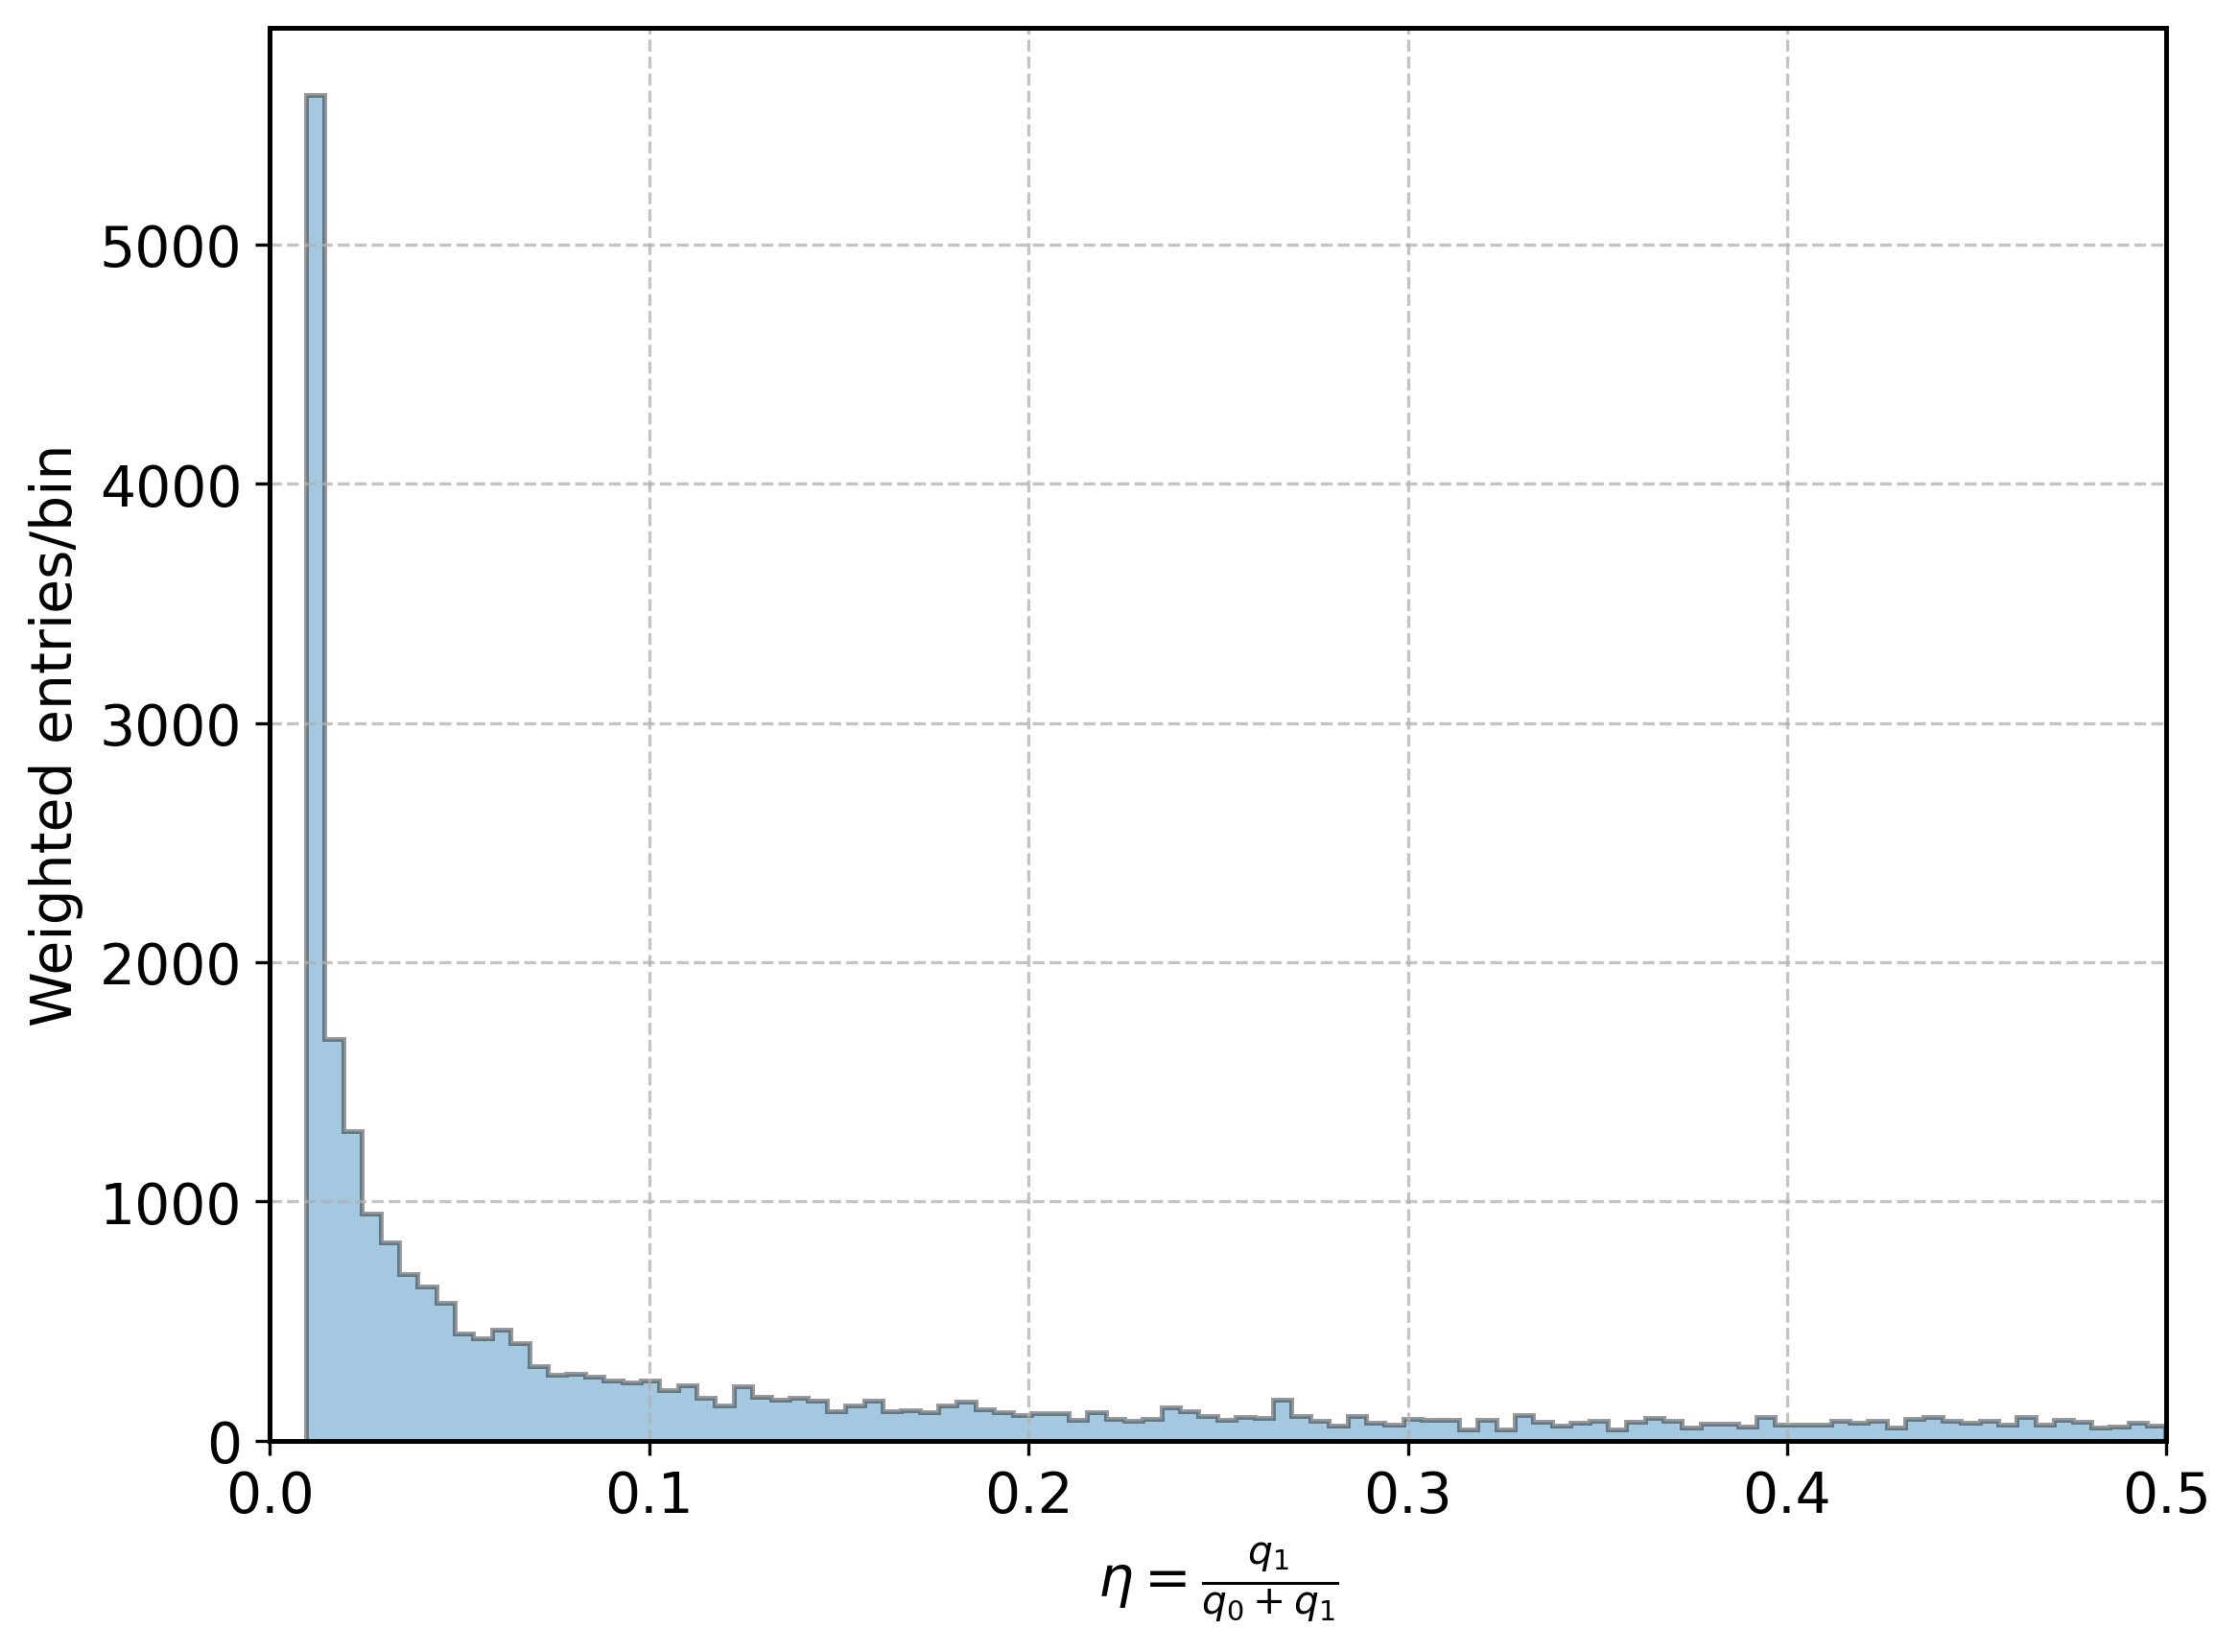
\includegraphics[width=0.49\linewidth]{figures/chapter4/position/eta_hist}
    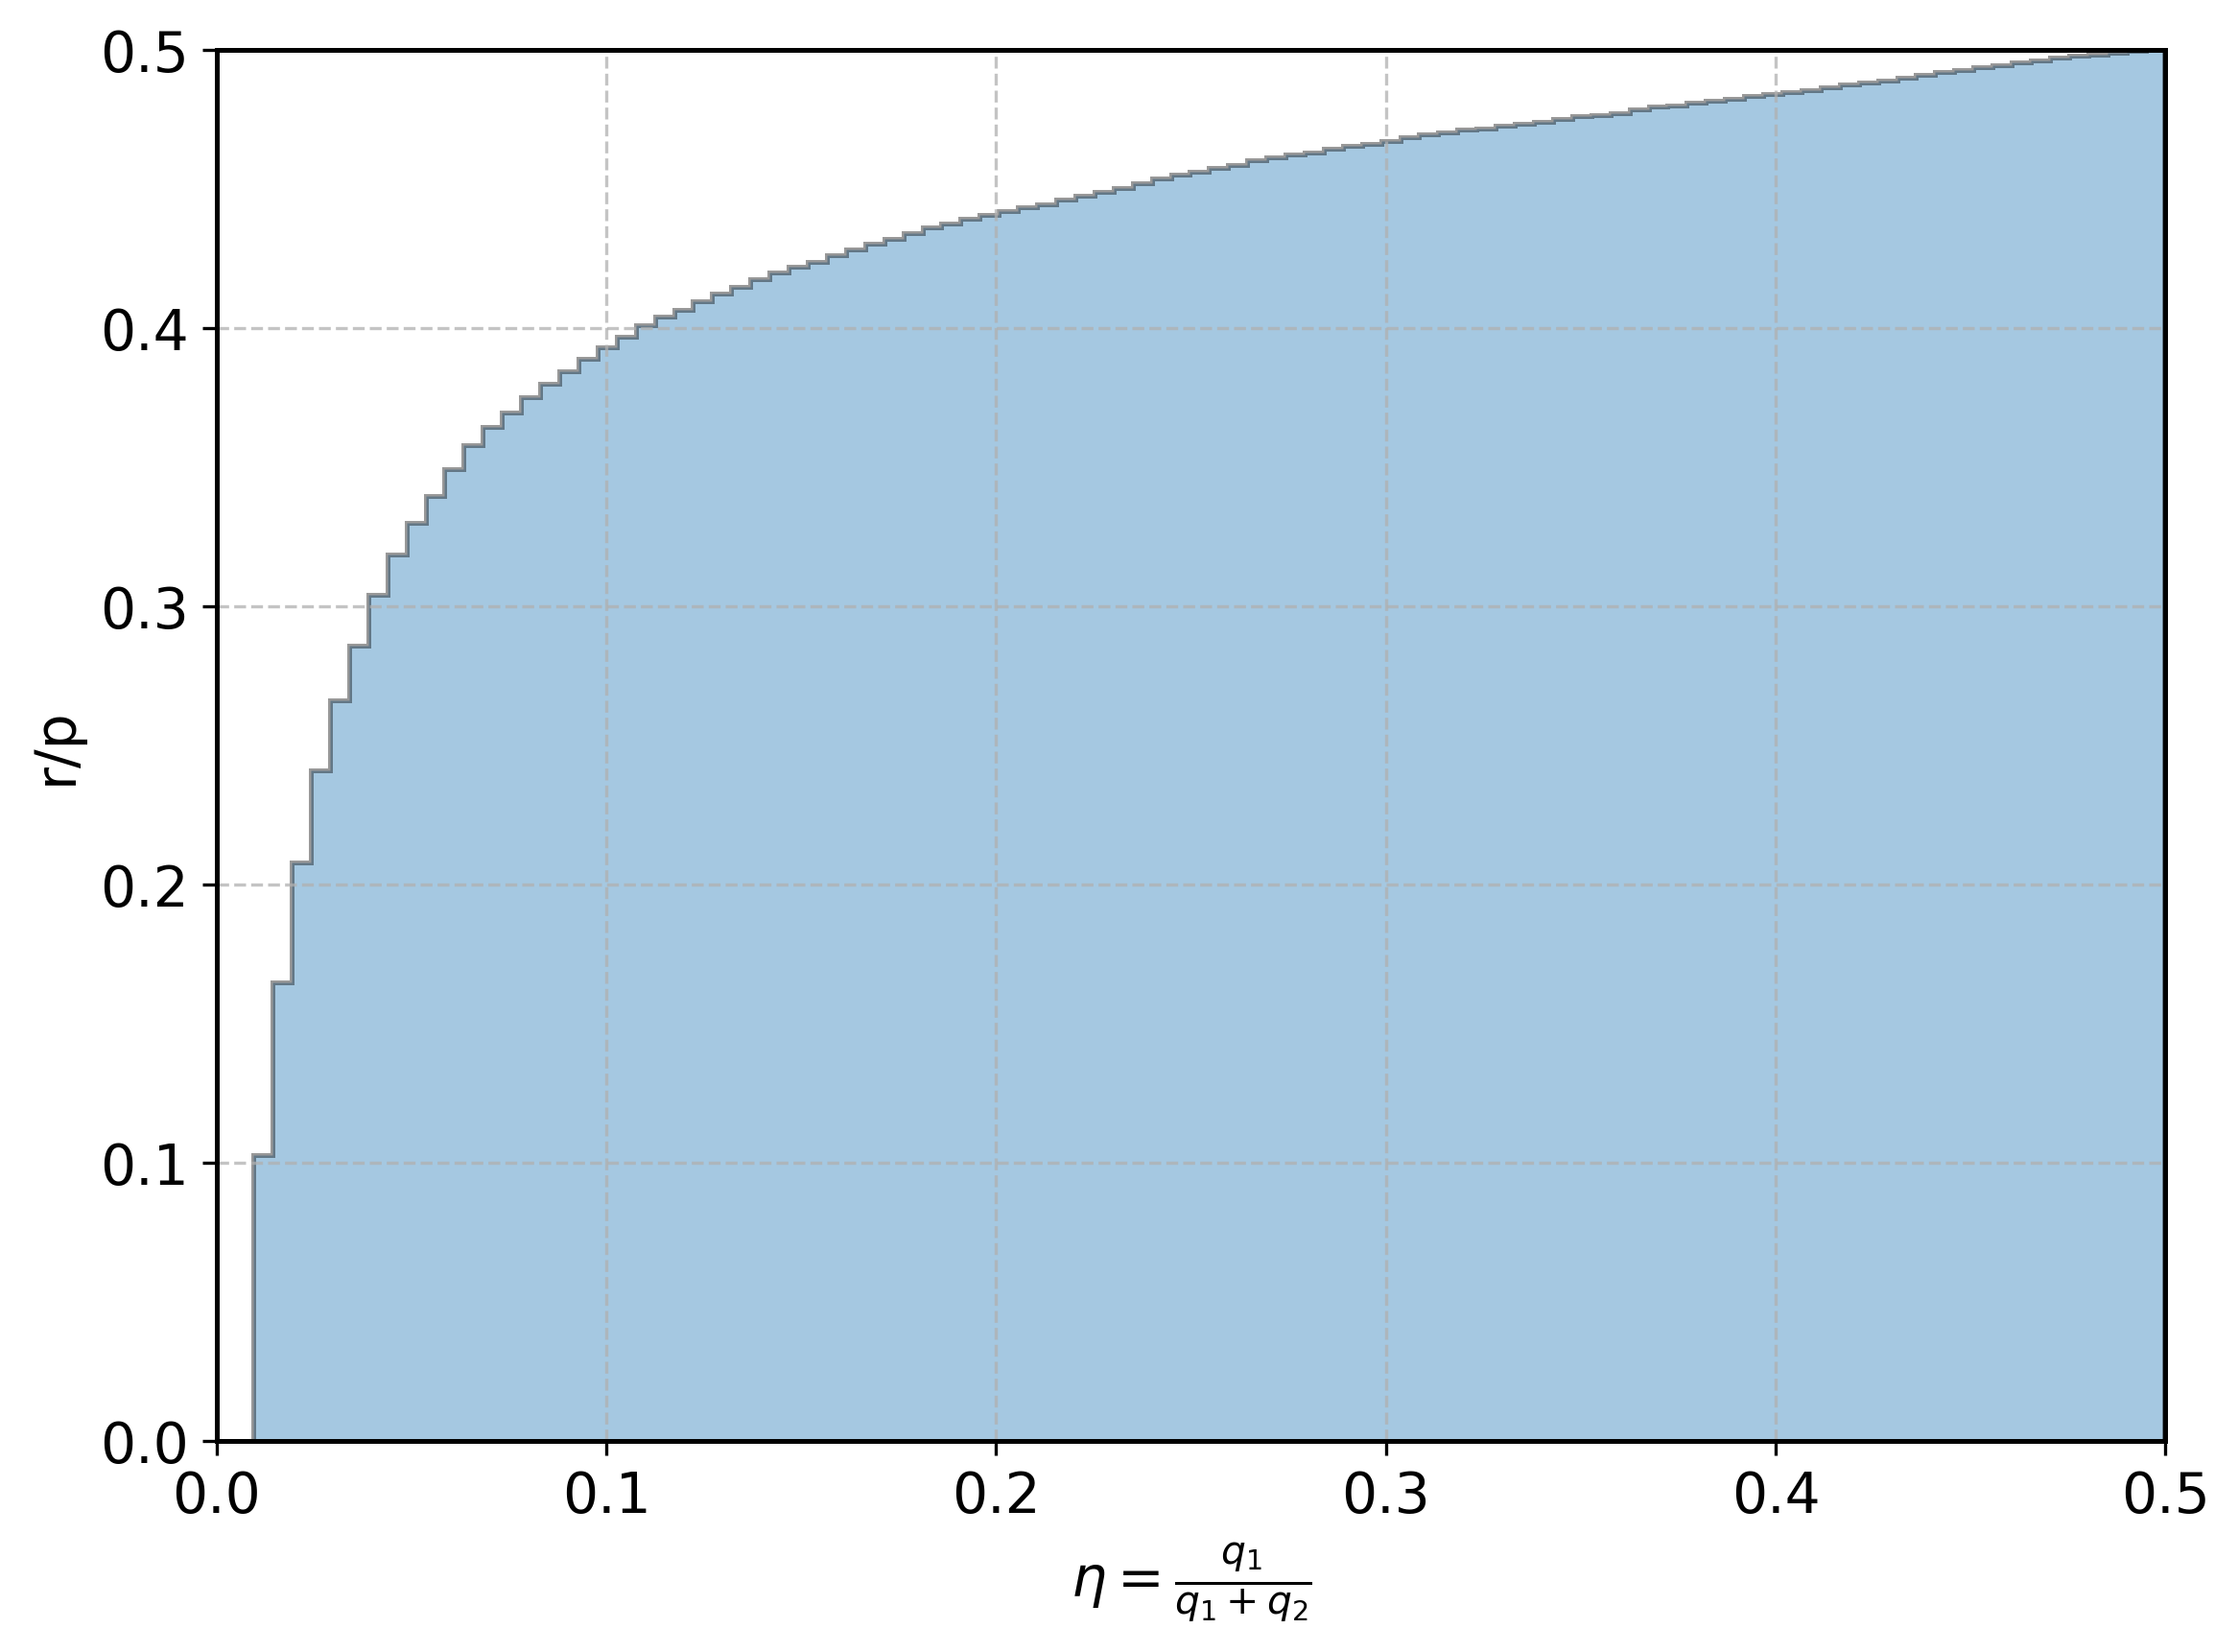
\includegraphics[width=0.49\linewidth]{figures/chapter4/position/eta_cumulative}
    \caption{$\eta$ distribution (left panel) after correcting for non-uniformity of event distribution and its cumulative distribution (right panel) for two-pixel events. The two distributions are truncated near $\eta=0$ because of a zero-suppression threshold that is applied.}
    \label{fig:eta_2pix}
\end{figure}

The cumulative distribution of this weighted histogram is calculated, which gives the updated non-linear relation $r_{n+1}(\eta)$

\begin{equation}
r_{n+1}(\eta) = r_{\textrm{min}} + (r_{\textrm{max}} - r_{\textrm{min}}) \frac{\int_{\eta_{\textrm{min}}}^{\eta} g_{n+1}(\eta') \, d\eta'}{\int_{\eta_{\textrm{min}}}^{\eta_{\textrm{max}}} g_{n+1}(\eta') \, d\eta'}.
\end{equation}

Using this relation, the steps are repeated. The resulting distributions are shown in Fig. \ref{fig:eta_2pix}. Finally, for event reconstruction, the cumulative distribution is interpolated to get a continuous function $r(\eta)$.

This approach can be generalized to the case of three-pixels events as well. Contrary to the two-pixels case, this is a two-dimensional problem. A single $\eta$ variable is not enough and the generalization of the previous case is to define the variables

\begin{equation}
\eta_1 = \frac{q_1}{q_0 + q_1 + q_2}, \quad \quad \eta_2 = \frac{q_2}{q_0 + q_1 + q_2}, \quad \quad q_0 > q_1 > q_2.
\label{eq:eta_3pix}
\end{equation}

\begin{figure}[!b]
    \centering
    \begin{tikzpicture}[scale=3]
    \hexpix{\hexsize}
    \node[anchor=south] at (0, 0) {$q_0$};
    \draw[|-|] (0, 0.75) -- (1, 0.75);
    \node[anchor=south] at (0.5, 0.75) {$p$};
    \begin{scope}
        \clip (0,0) -- (0:\hexsize) -- (-30:\hexsize) -- cycle;
        \fill[pattern=north east lines, pattern color=gray] (-1,-1) rectangle (1,1);
    \end{scope}
    \hexpix[xshift=1cm]{\hexsize}
    \node[anchor=south] at (1, 0) {$q_1$};
    \hexpix[xshift=0.5cm, yshift=-0.866cm]{\hexsize}
    \node[anchor=north] at (0.5, -0.866) {$q_2$};
    \draw[dashed] (0, 0) -- (1, 0);
    \draw[->] (0, 0) -- (1.5, -0.866);
    \draw[dashed] (0, 0) -- (0.5, -0.866);
    \draw[dashed] (0.5, -0.866) -- (1, 0);
    \draw[dashed] (0, 0) -- (1.7, -0.45);
    \node[anchor=west] at (1.5, -0.866) {$r$};
    \draw[->] (1.45, -0.827) arc[start angle=-30, end angle=-10, radius=1.2];
    \node[anchor=west] at (1.55, -0.65) {$\theta$};
    \end{tikzpicture}
    \caption{Illustration of the three-pixel event topology. Assuming that the ordering
    of the charges is $q_2 \leq q_1 \leq q_0$, the hatched triangle represents again the 
    portion of the phase space in terms of the true impact point originating this topology.}
    \label{fig:three_pixel_event}
\end{figure}

These two new variables are still not good enough, because it is not easy to parametrize the geometry of the problem with them. By looking at the geometry of the three pixels in Fig. \ref{fig:three_pixel_event}, a better parametrization can be employed to simplify the description of this type of events.

The idea is to decompose the two-dimensional problem into two one-dimensional problems that can be treated as two-pixel events, each describing a specific coordinate. The best coordinates for this problem 
are a radial coordinate and an angular coordinate. The two coordinates are defined as follows:
\begin{itemize}[label=-]
\item $r$ is distance of the incident position projected onto the axis that passes through the vertex of the central pixel and the middle point between the outer pixels centers;
\item $\theta$ is the angle measured starting from the latter axis and oriented towards the outer pixel with the highest charge collected.
\end{itemize}

Considering the ASIX readout geometry, where the central pixel is always the one with the highest pixel and the other two pixels are neighbors, the radial component can be parametrized as a two-pixel event by considering the outer pixels as a single pixel with charge equal to their sum. This automatically defines a new $\eta_+$ variable which is defined as

\begin{equation}
\eta_+ = \eta_1 + \eta_2.
\label{eq:eta_sum}
\end{equation}

\begin{figure}[!t]
    \centering
    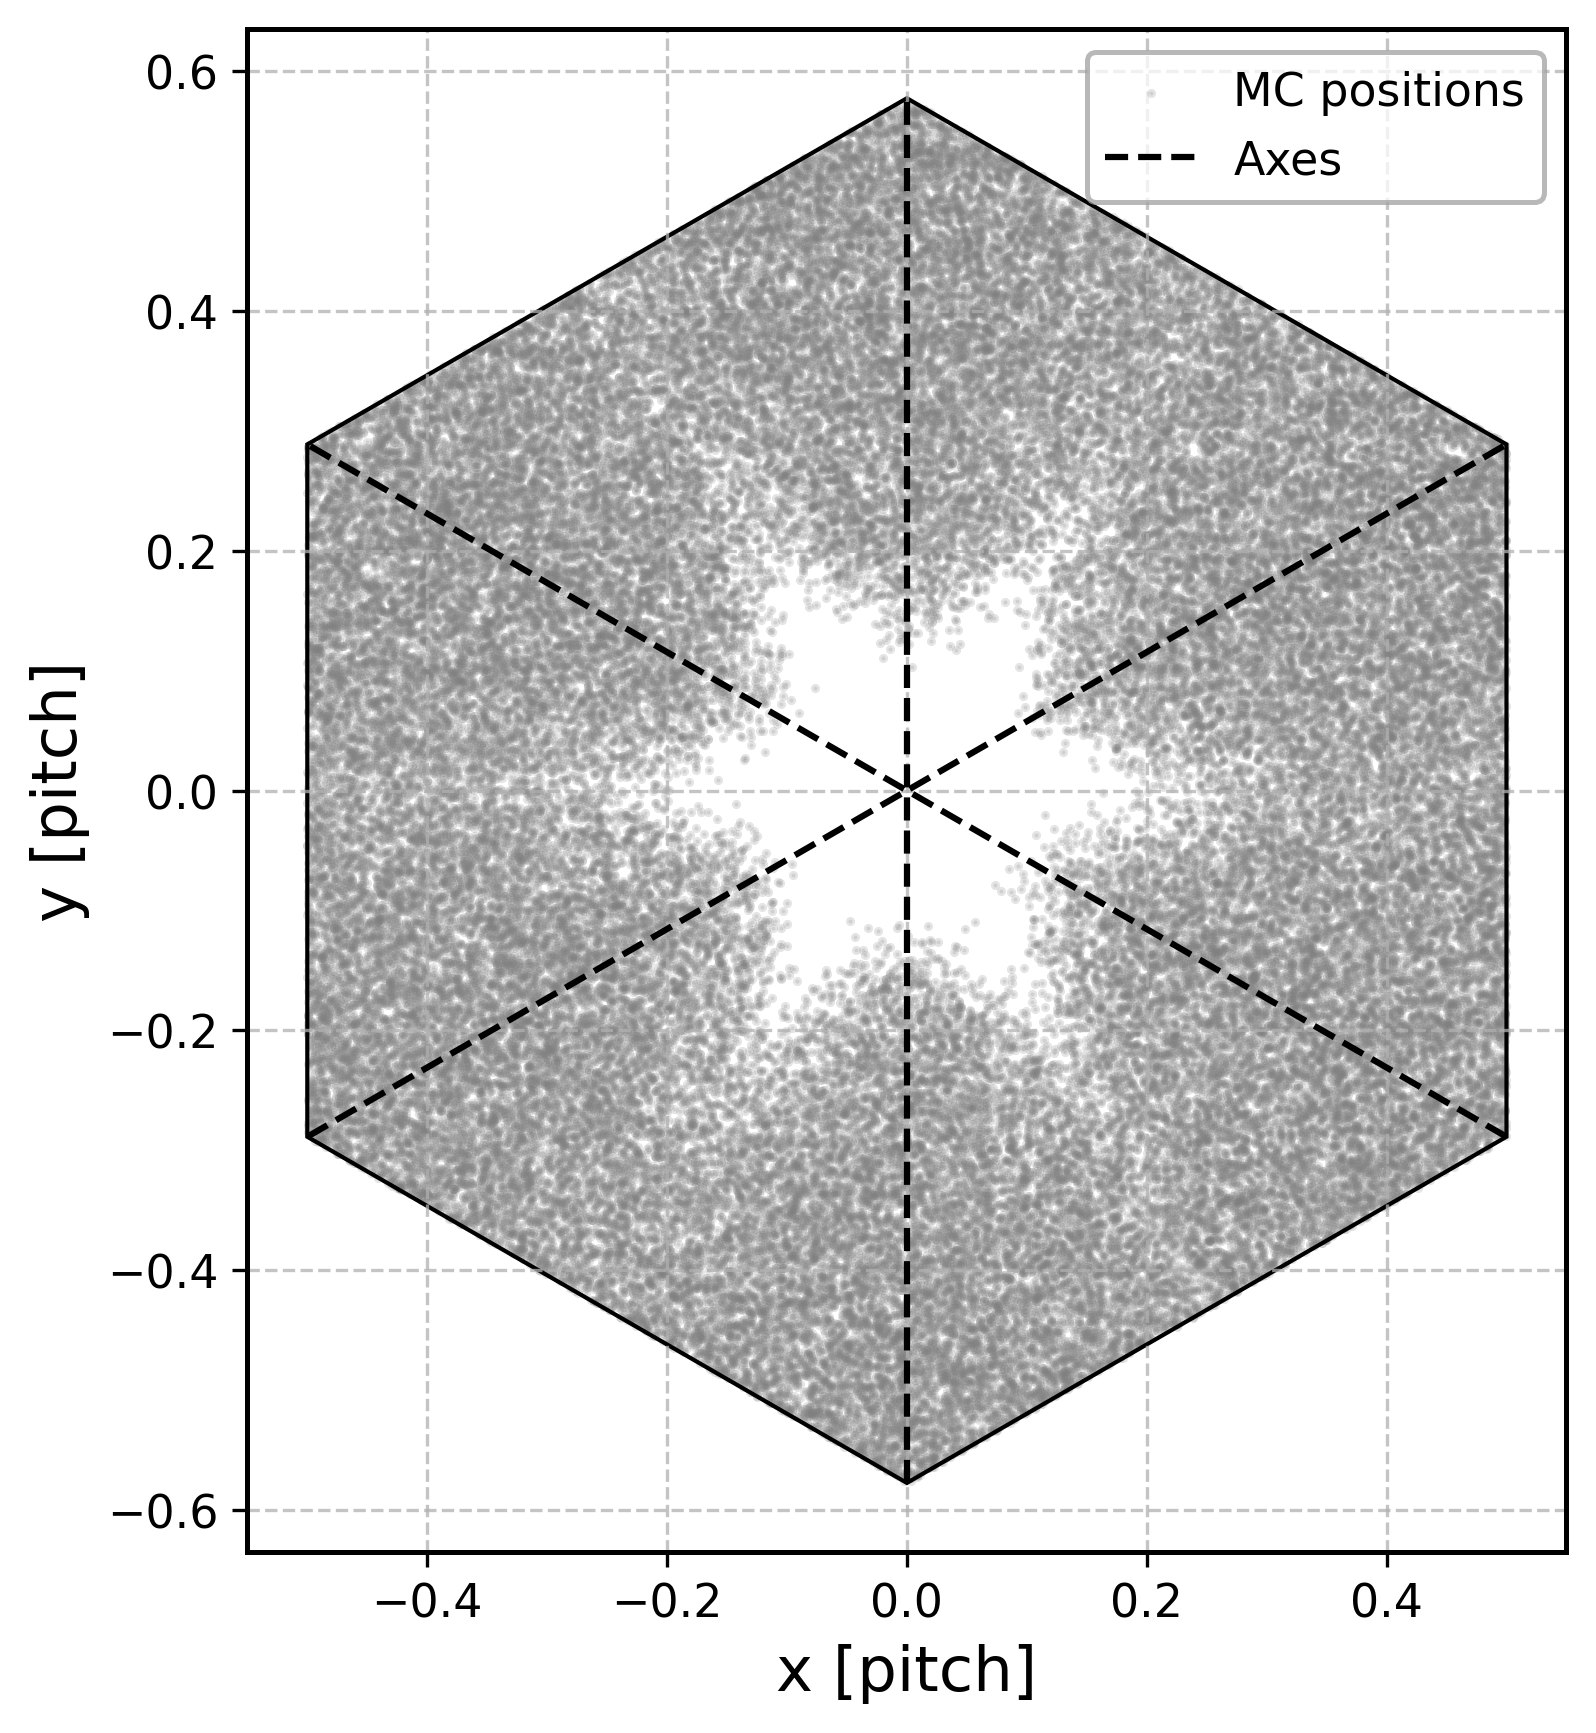
\includegraphics[width=0.35\linewidth]{figures/chapter4/position/eta_3pix_scatter}
    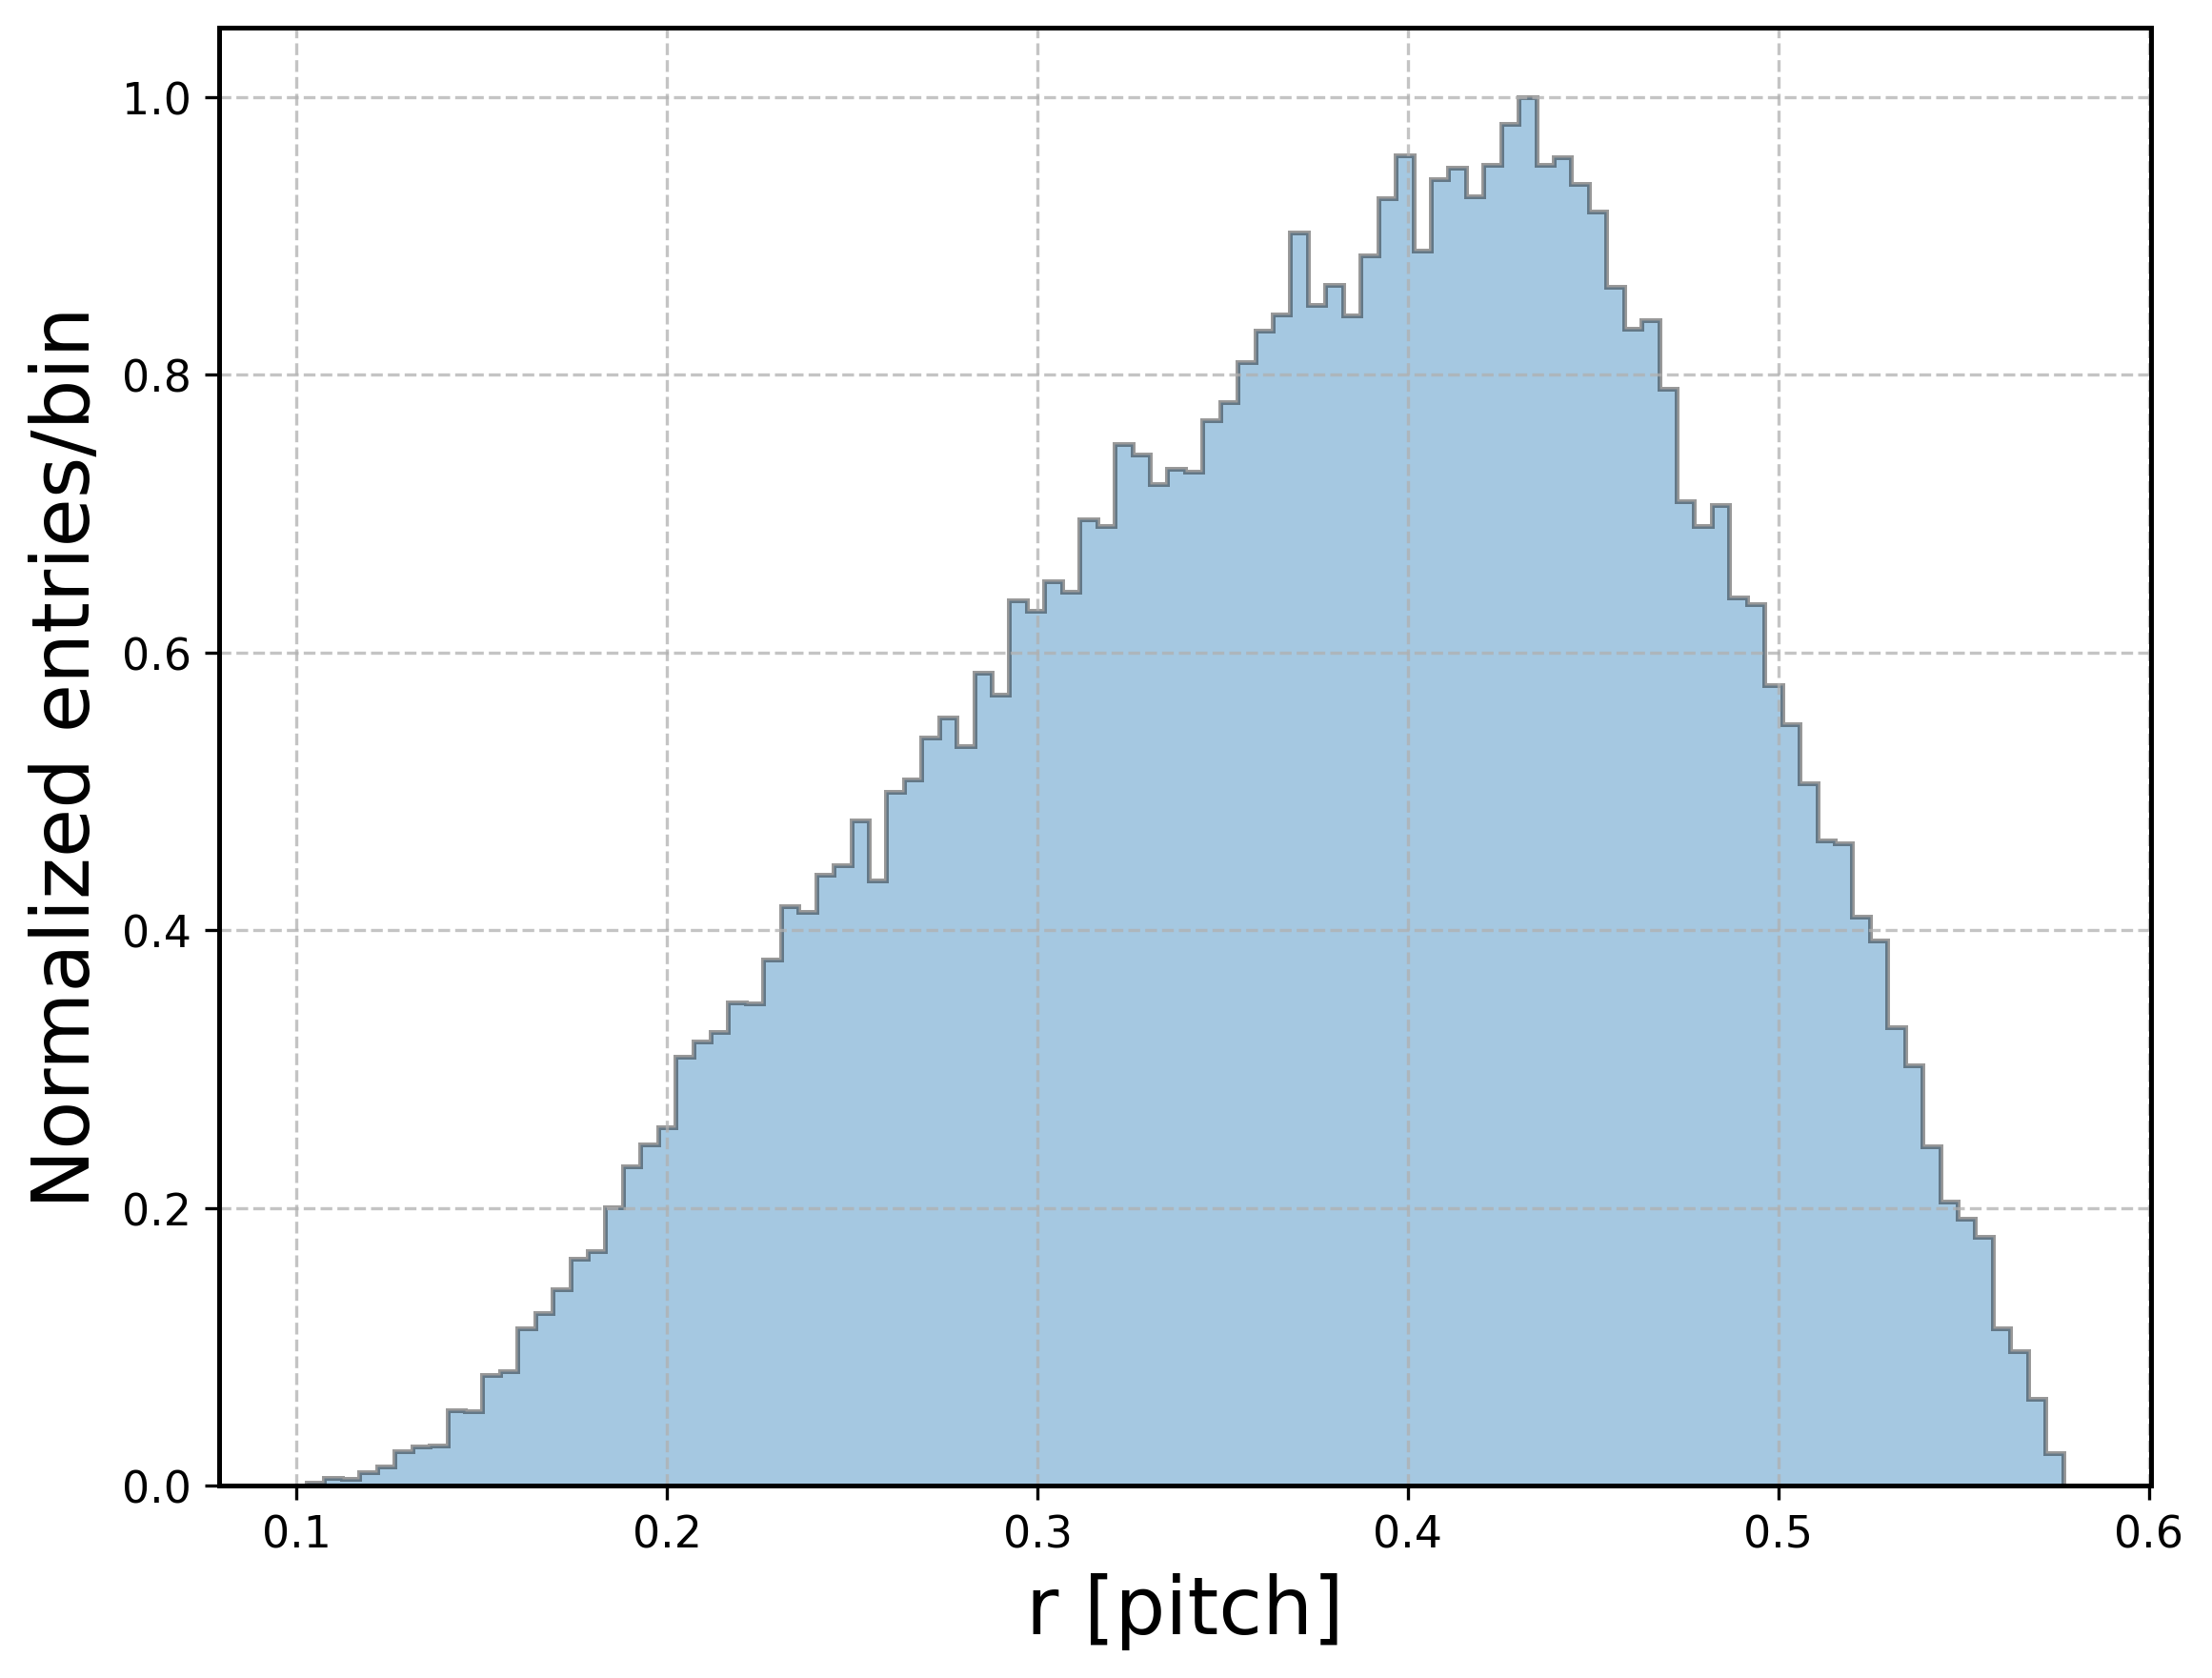
\includegraphics[width=0.49\linewidth]{figures/chapter4/position/eta_3pix_dr_hist}
    \caption{Scatter plot of Monte Carlo truth impact positions of three-pixel events on the central pixel (left panel) and event count distribution of the events projected onto the radial axes, shown with dashed lines (right panel). The empty circular region at the center of the hexagon is where events are labeled as one-pixel events, and its radius depends on the zero-suppression threshold.}
    \label{fig:3pix_scatter}
\end{figure}

The angular coordinate can be parametrized as a two-pixel event problem as well. In this case the relevant property is how the charge collected by the outer pixels is divided between them. As a consequence, a new variable can be defined as

\begin{equation}
\eta_- = \frac{\eta_1 - \eta_2}{\eta_+}.
\label{eq:eta_minus}
\end{equation}

\begin{figure}[!b]
    \centering
    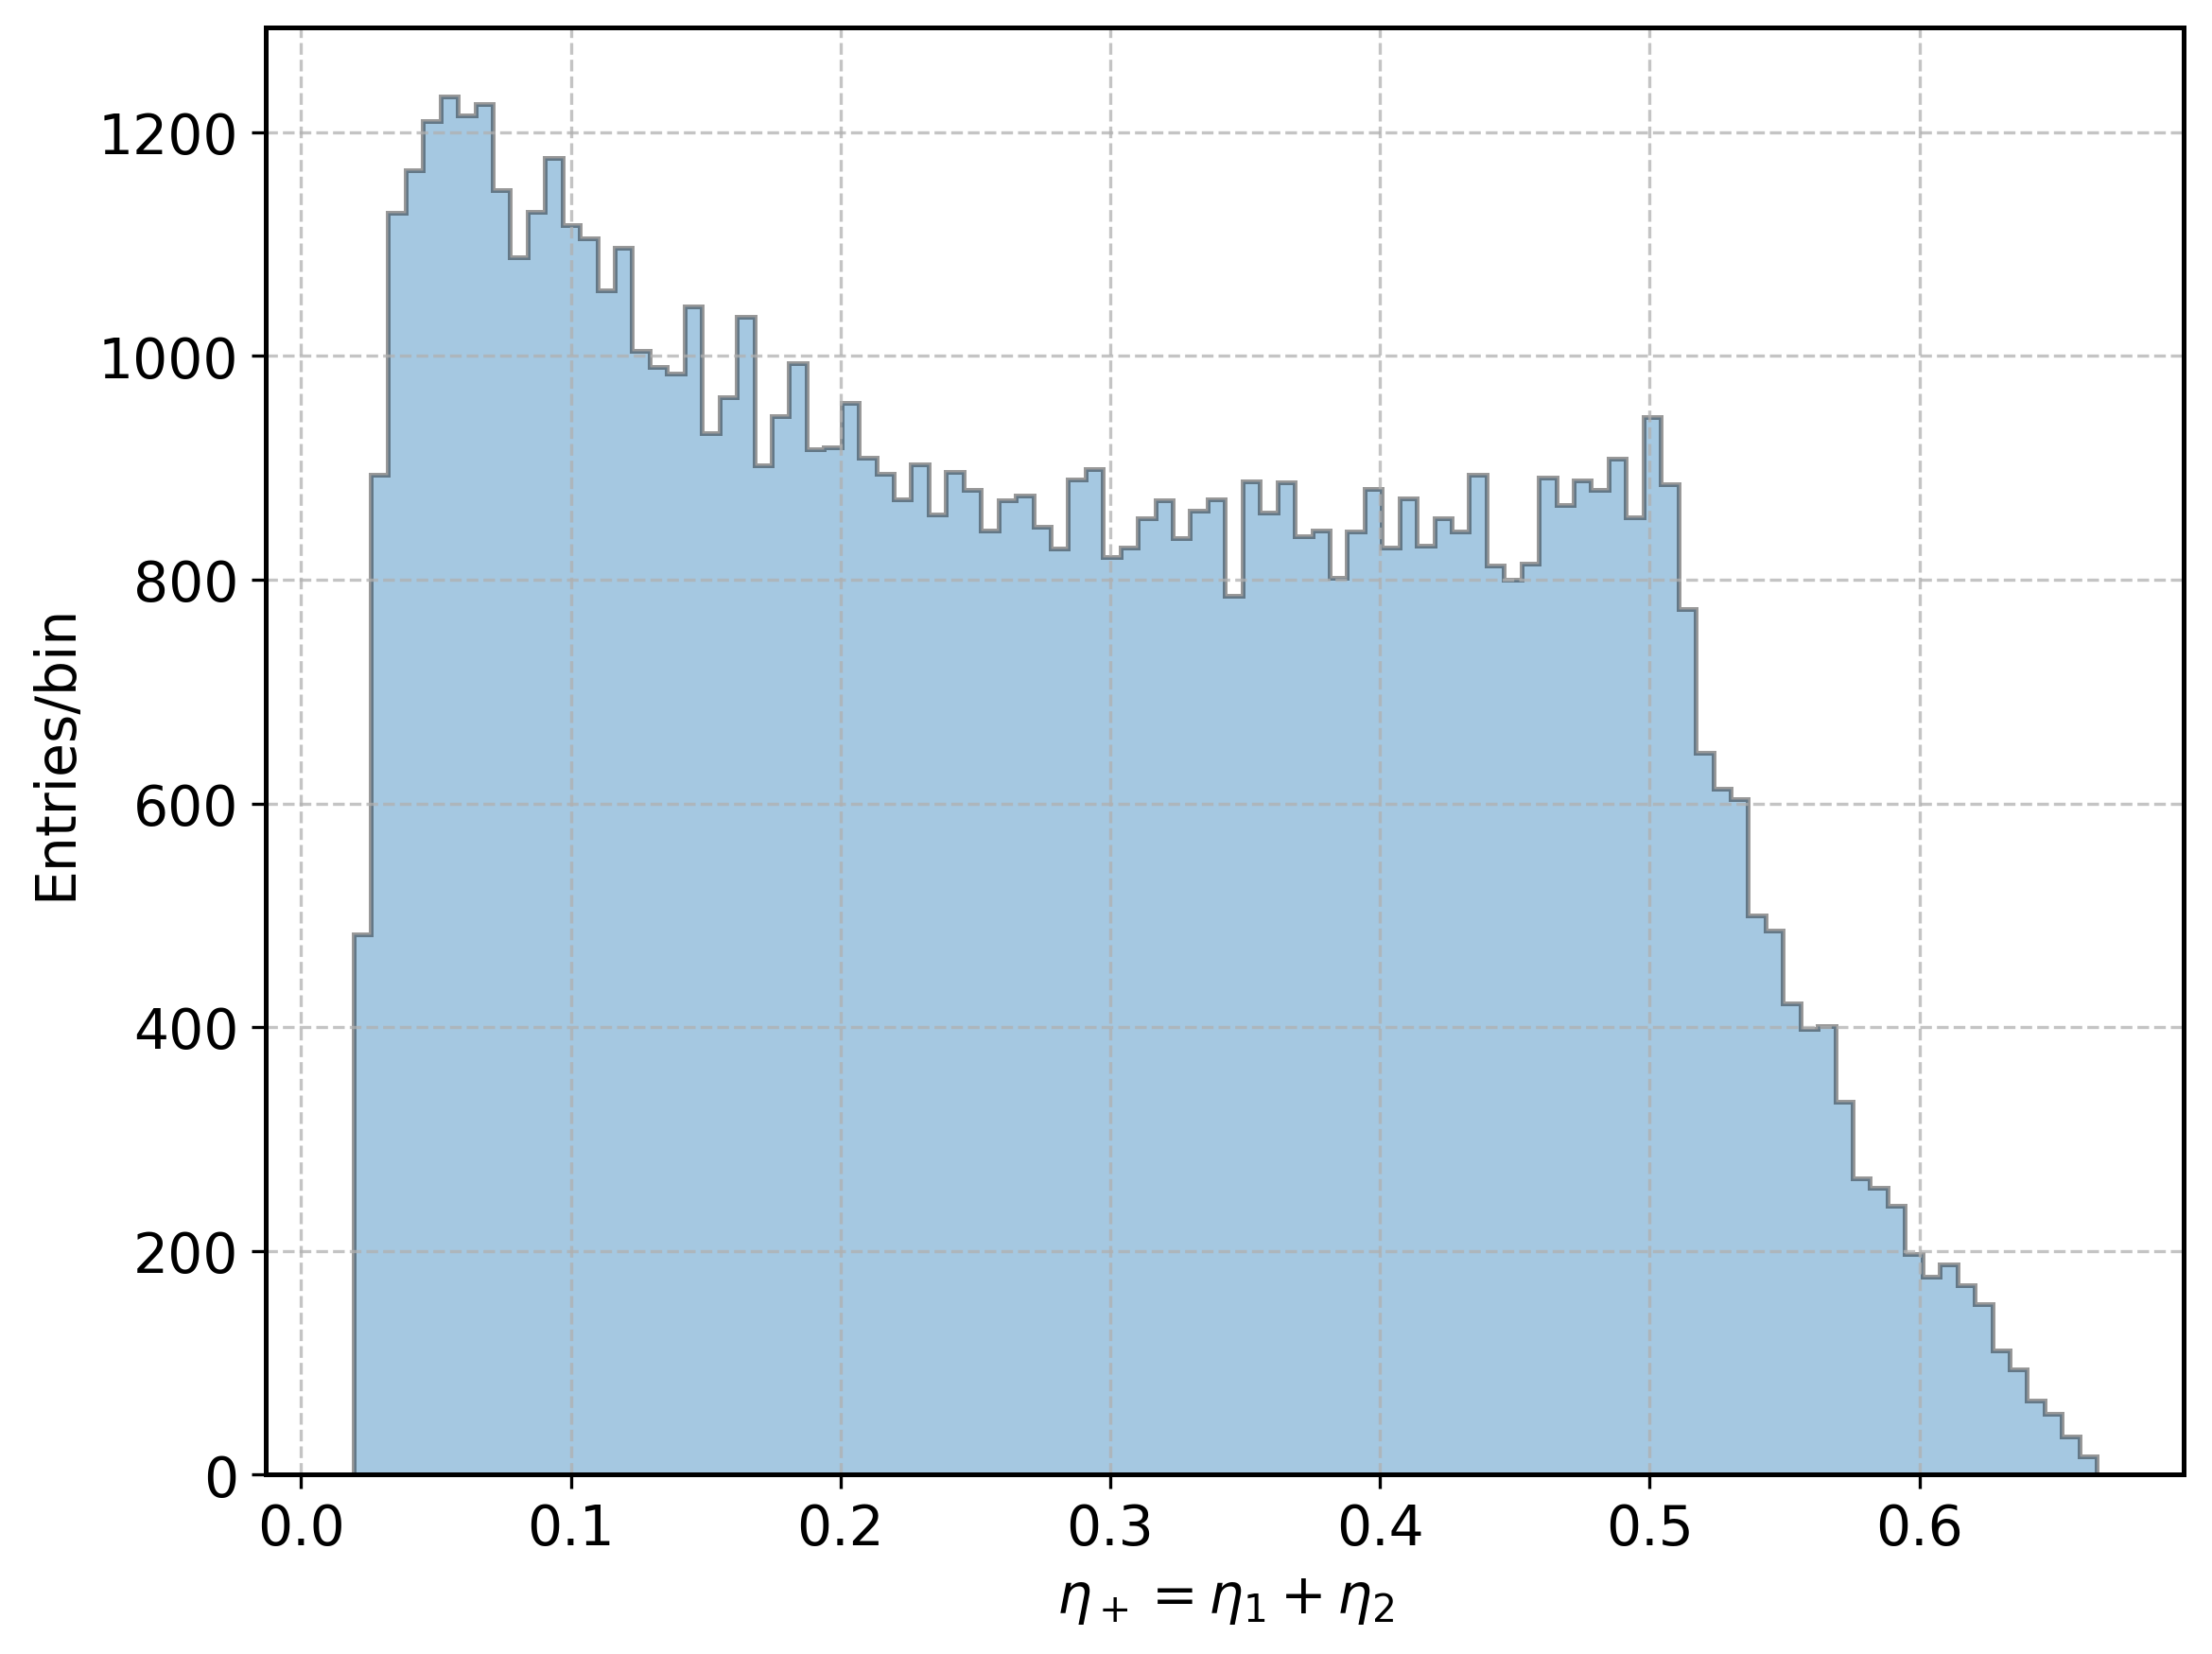
\includegraphics[width=0.49\linewidth]{figures/chapter4/position/eta_3pix_uncorrected_hist}
    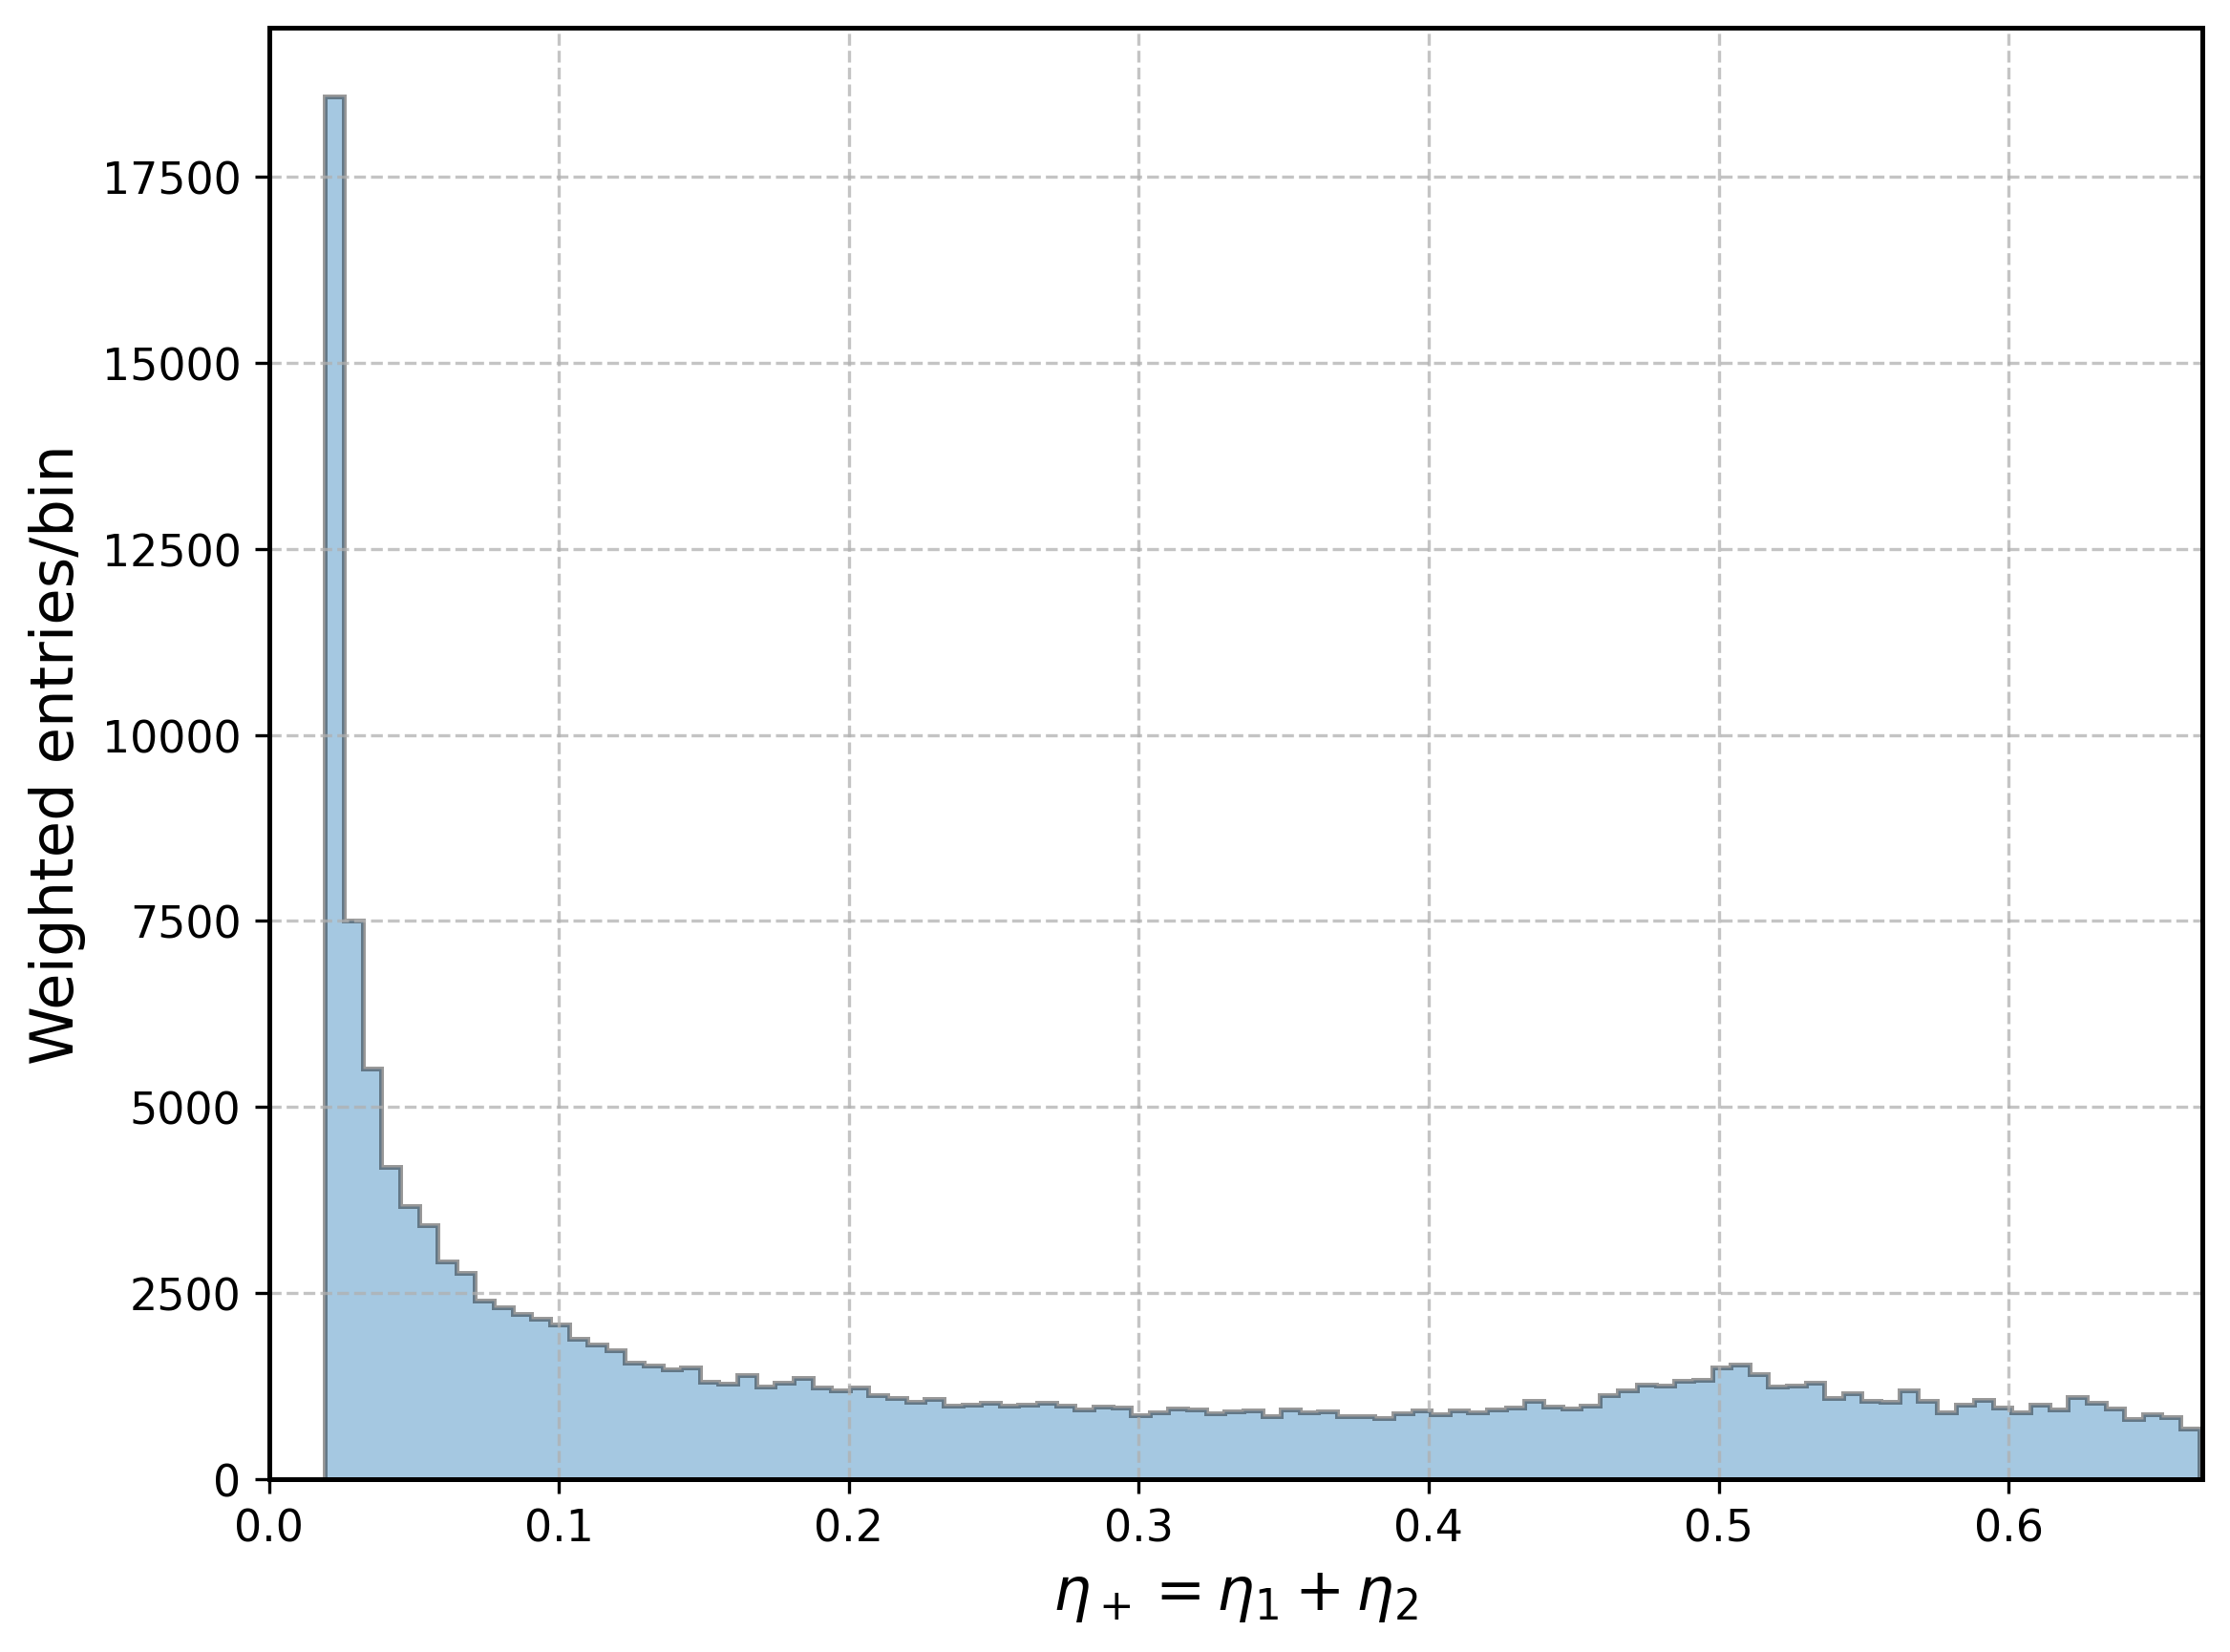
\includegraphics[width=0.49\linewidth]{figures/chapter4/position/eta_3pix_rad_hist}
    \caption{$\eta_+$ distribution without weigthing the entries to correct for non-uniformity (left panel) and distribution with the correction applied (right panel). $\eta_-$ distribution is not shown, but the distorsion in the uncorrected distribution is of a similar magnitude.}
    \label{fig:3pix_rad_eta}
\end{figure}

As in the case of two-pixel events, the uniformity of the events along the relevant axes has to be verified and, in case, corrected. The scatter plot of the Monte Carlo truth incidence positions and their distribution along the radial axis for three-pixel events are shown in Fig. \ref{fig:3pix_scatter}. It is possible to see that the distribution is highly non-uniform.

\begin{figure}[!t]
    \centering
    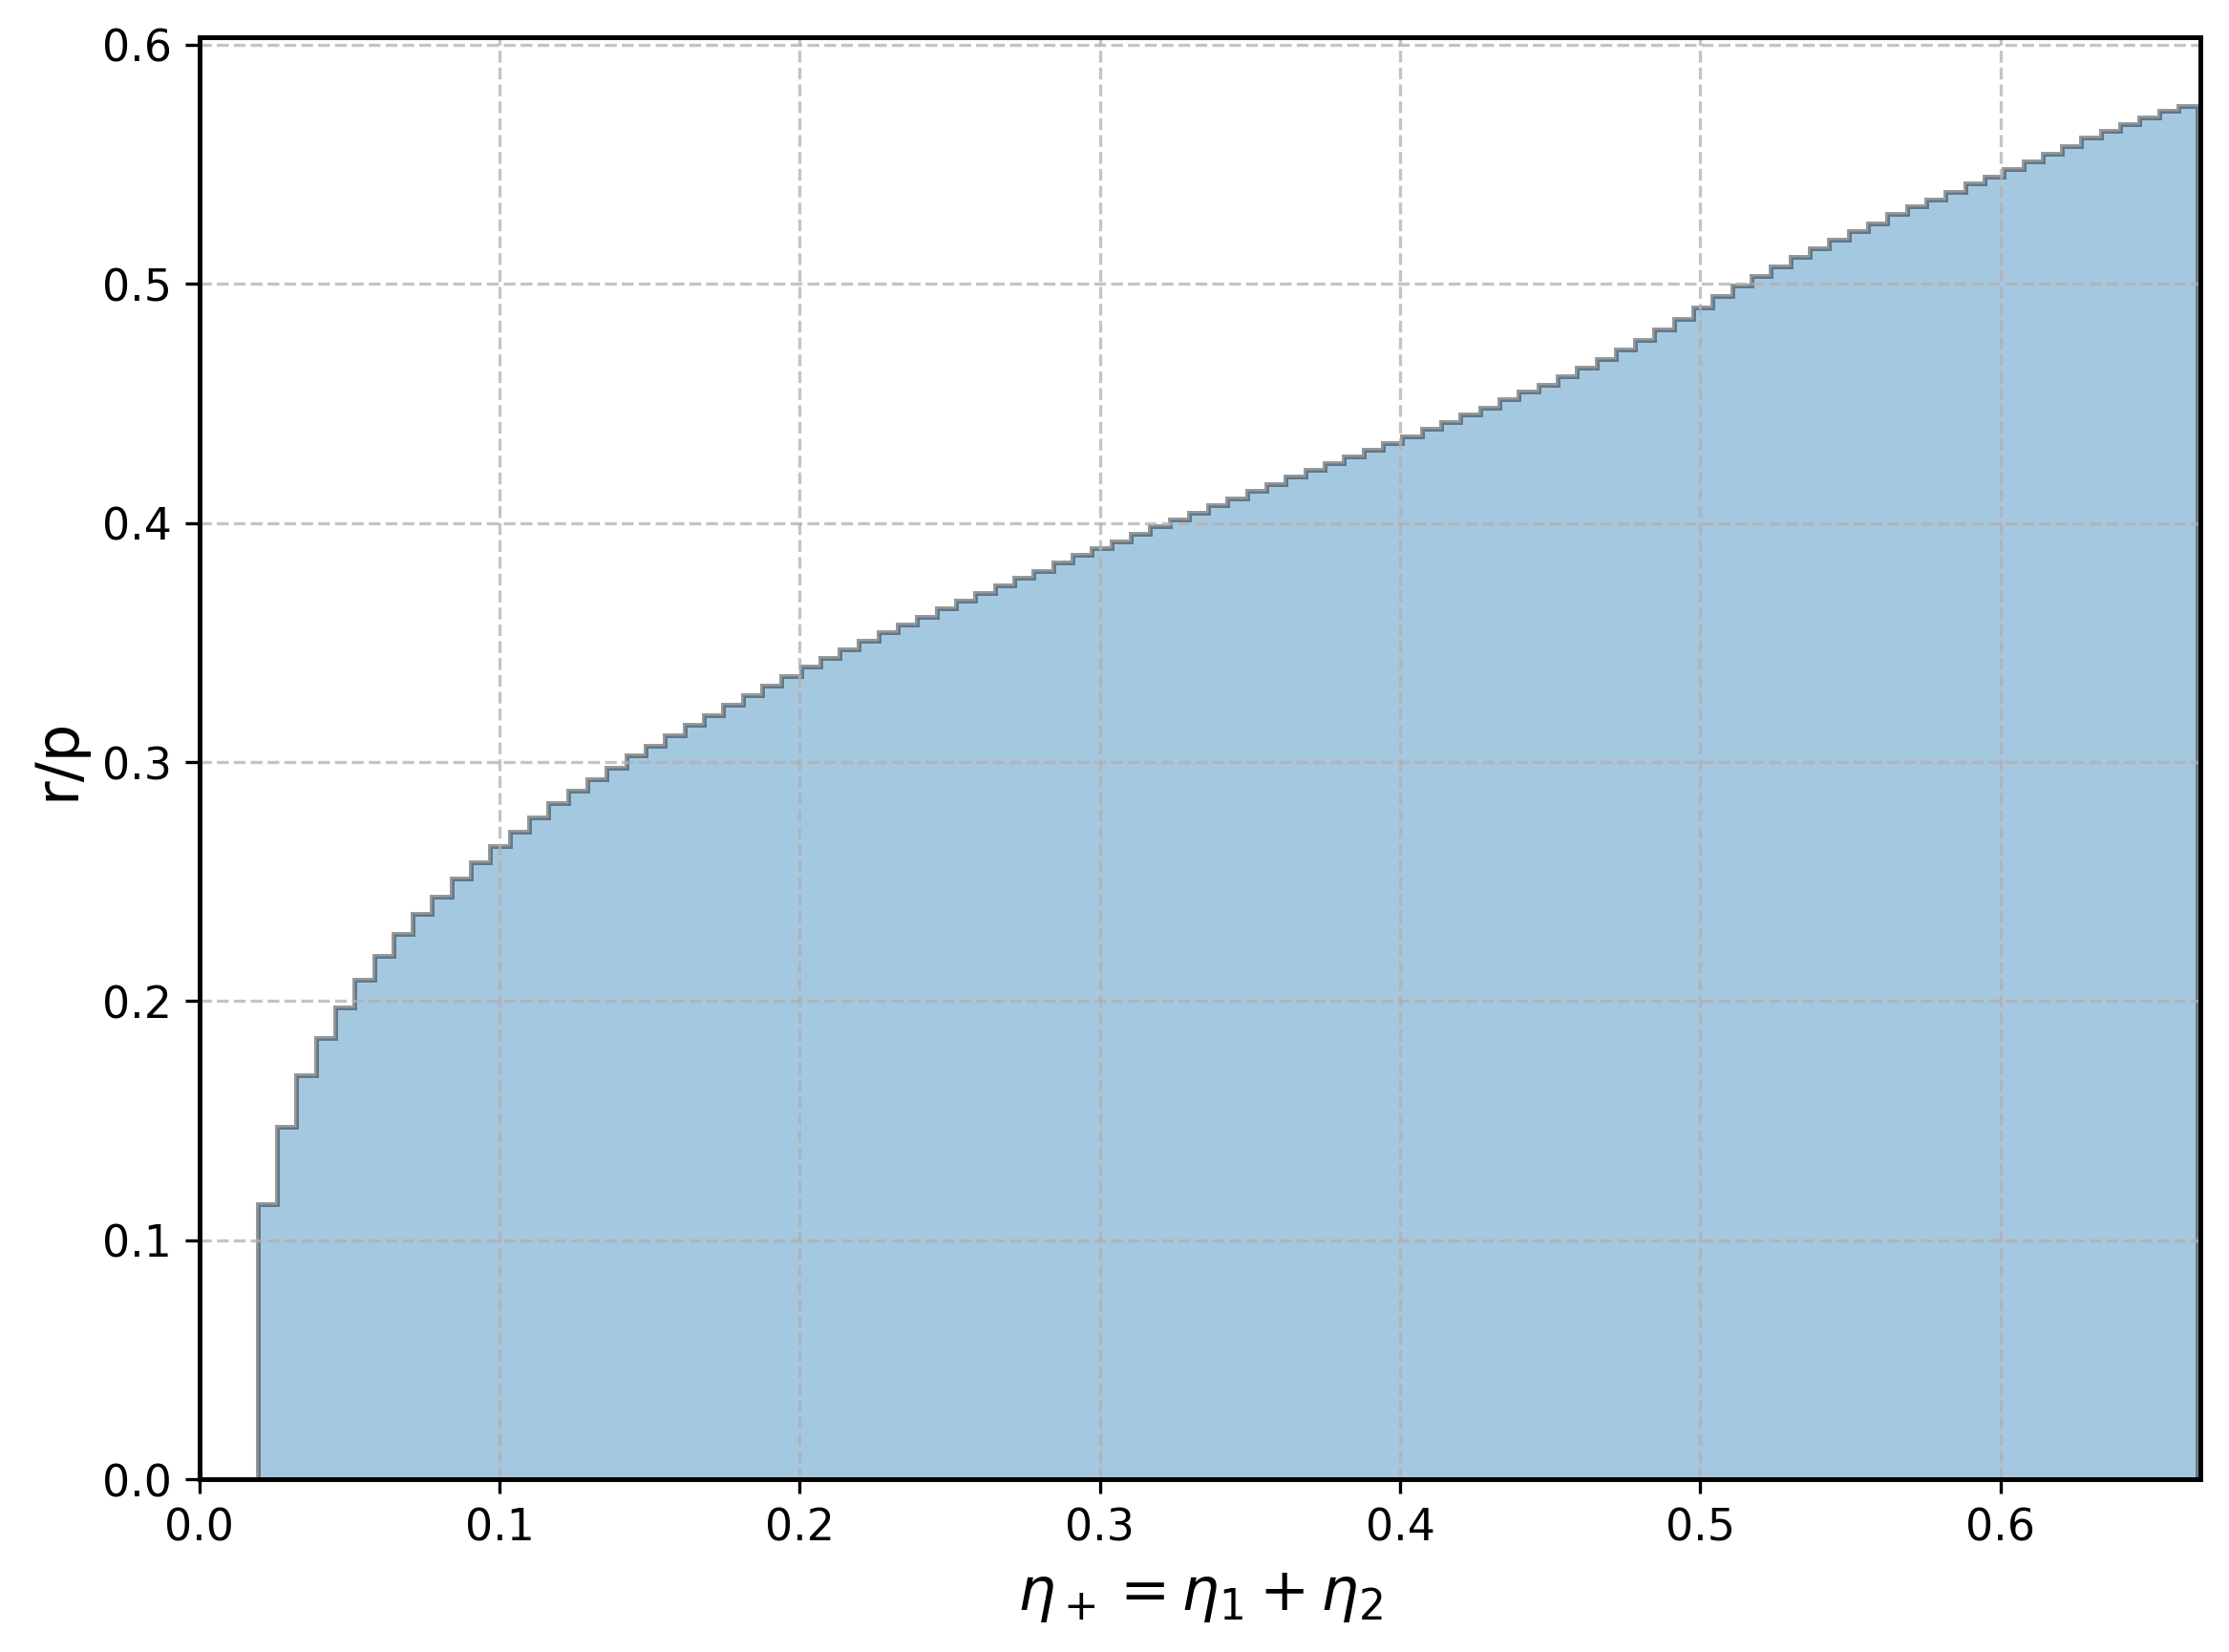
\includegraphics[width=0.49\linewidth]{figures/chapter4/position/eta_3pix_rad_cumulative}
    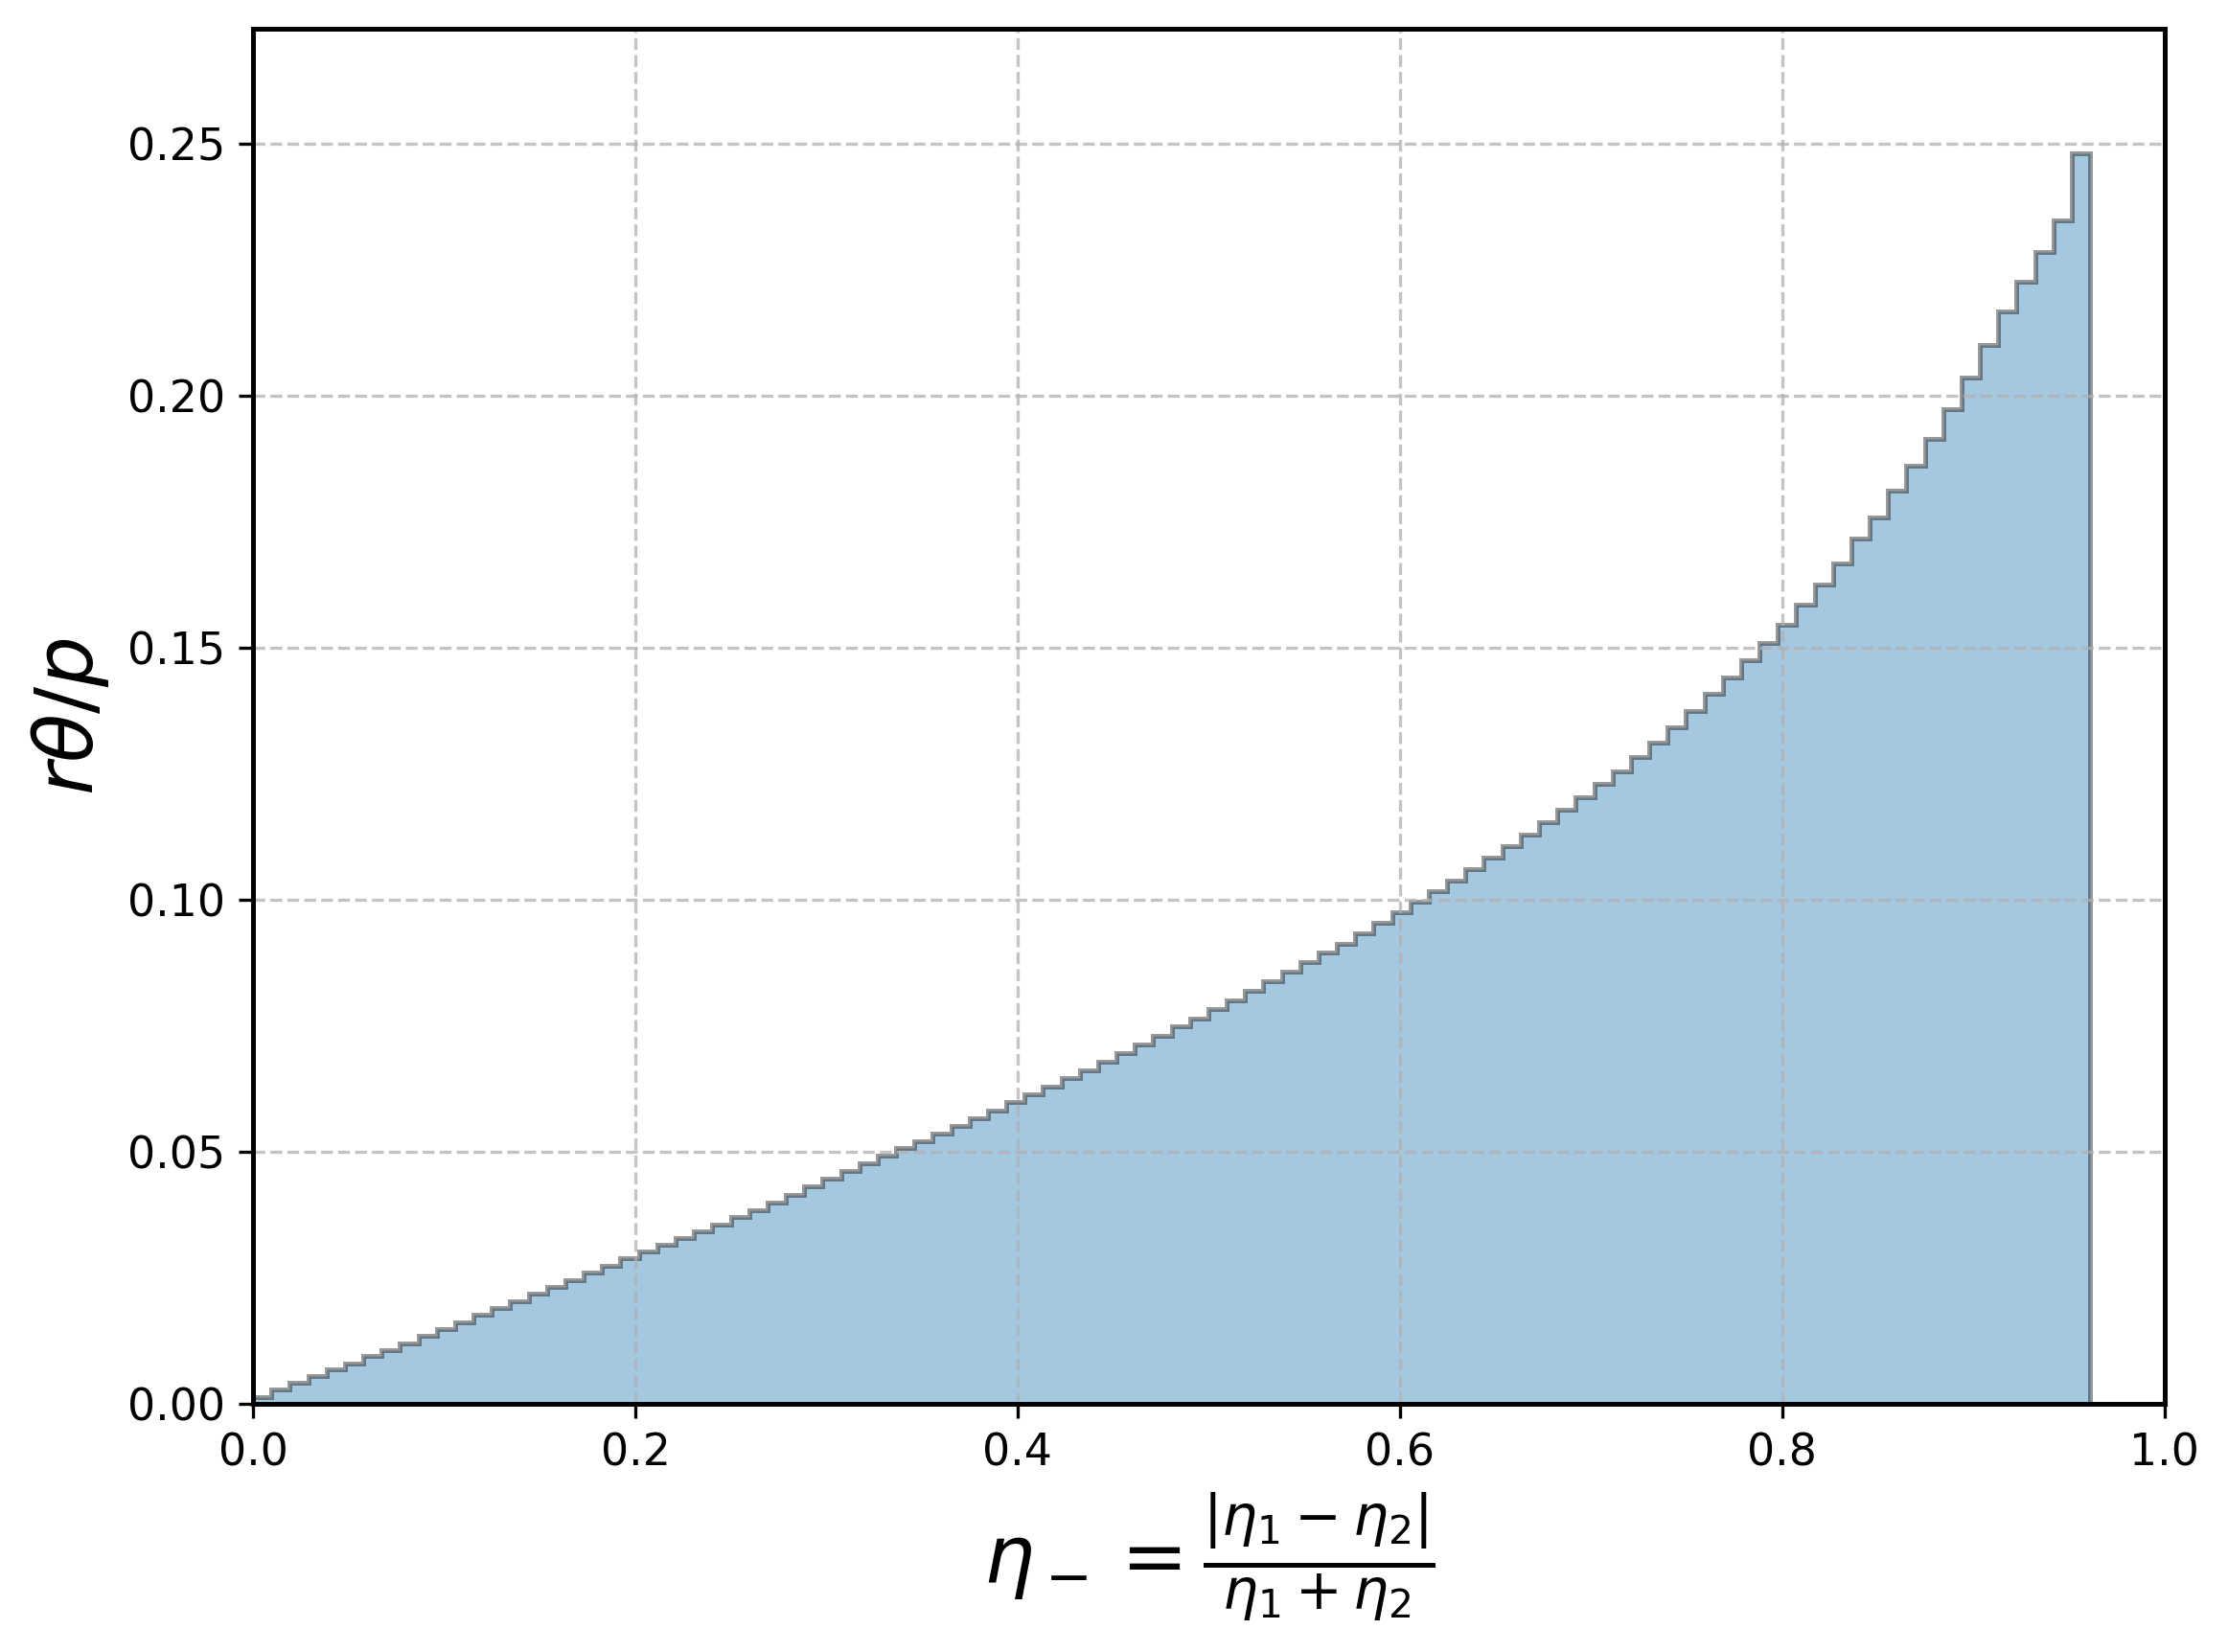
\includegraphics[width=0.49\linewidth]{figures/chapter4/position/eta_3pix_ang_cumulative}
    \caption{Cumulative distributions for $\eta_+$ (left panel) and $\eta_-$ (right panel) variables. }
    \label{fig:eta_3pix}
\end{figure}


For three-pixel events, the non-uniformity of the spatial distribution is primarily a geometrical effect. Even though the events are uniformly spread across the two-dimensional surface of the pixel, the transverse width of the relevant sector significantly varies along the reconstruction axis, reaching a peak after the middle point. This variation directly shapes the projected distribution, which is exactly what is observed in the left panel of Fig. \ref{fig:3pix_scatter}.

\begin{figure}[!b]
    \centering
    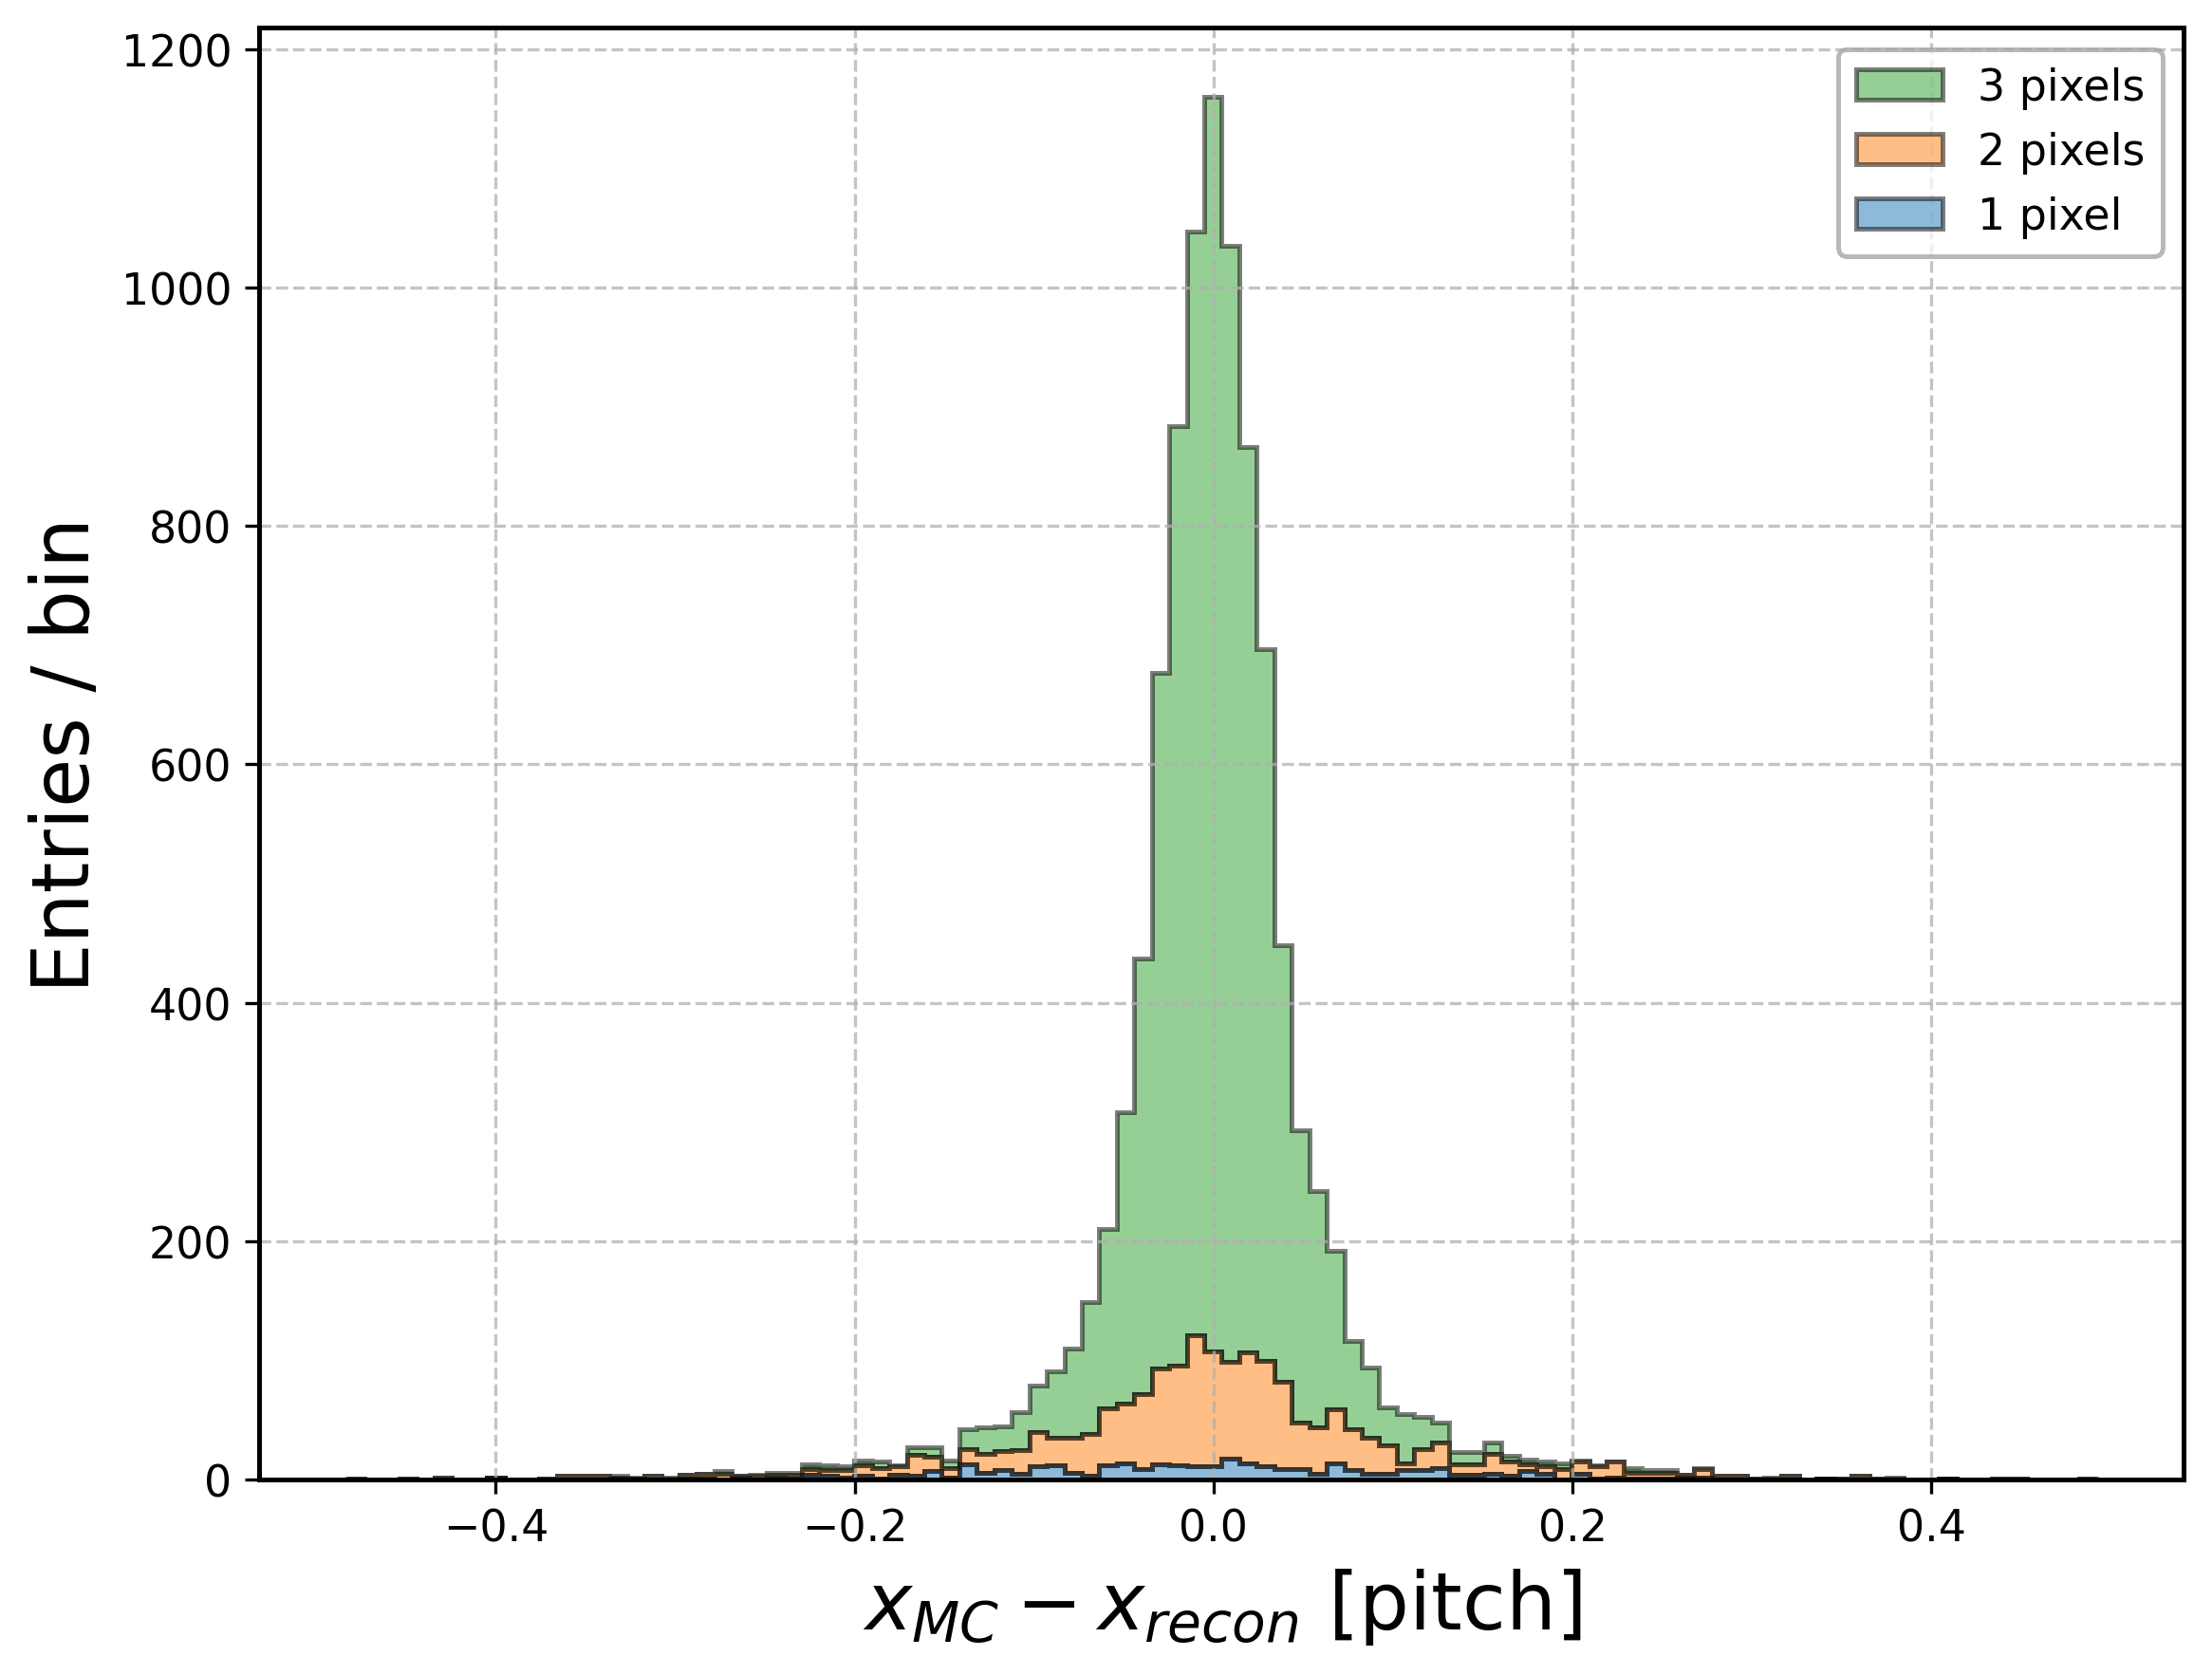
\includegraphics[width=0.49\linewidth]{figures/chapter4/position/eta_unmodeled_dx}
    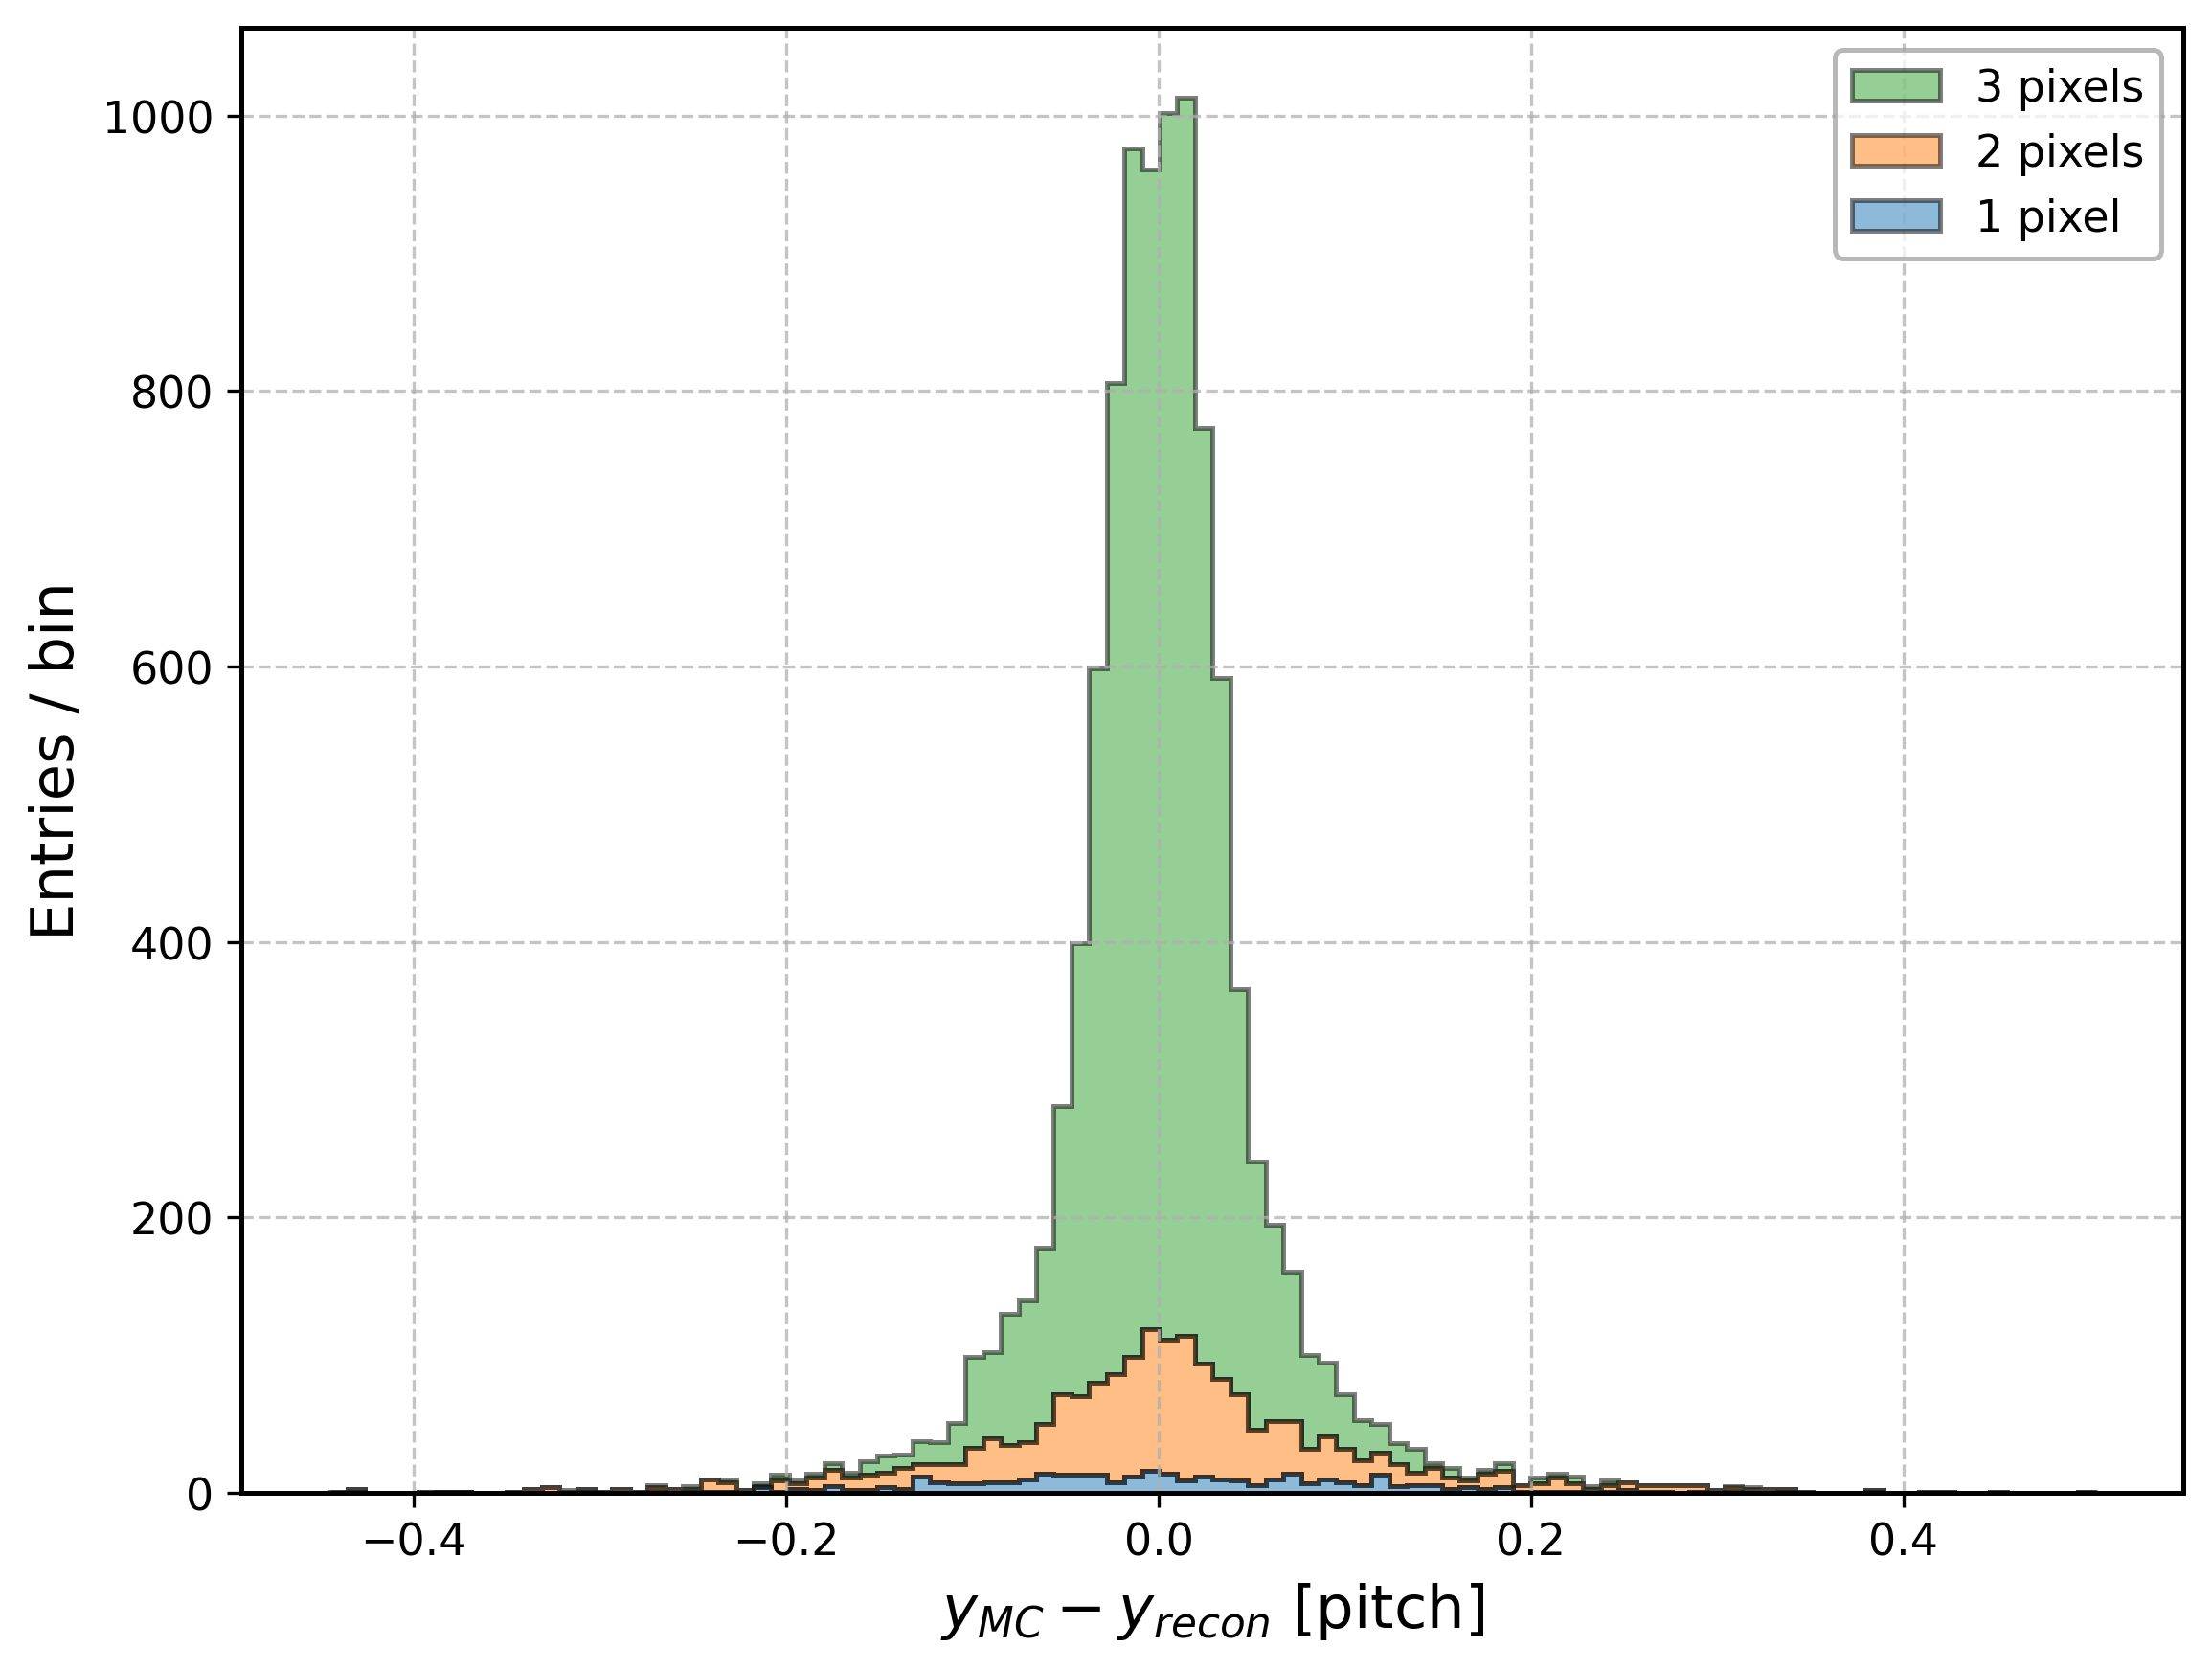
\includegraphics[width=0.49\linewidth]{figures/chapter4/position/eta_unmodeled_dy}
    \caption{Residuals distributions of the eta algorithm for the $x$ and $y$ directions, calculated as the difference between the reconstructed and the Monte Carlo truth $x$ and $y$ components. The events are separated by cluster size, with each color representing a specific cluster size. The histograms are stacked on each other. The simulation is made with a 8 keV monochromatic source, 20 ENC of noise and ratio between the diffused charge cloud sigma and the pitch of 15\%.}
    \label{fig:eta_dx_dy}
\end{figure}

A similar behaviour is observed for $\eta_-$ projecting onto the axis perpendicular to the radial one. These non-uniformities heavily affect the shape of $\eta_+$ and $\eta_-$ distributions. Fig. \ref{fig:3pix_rad_eta} shows a comparison between the $\eta_+$ with and without the correction for uniformity.

After correcting non-uniformities in the $\eta_+$ and $\eta_-$ distributions with the same iterative approach used for two-pixel events, the cumulative distributions can be calculated. The cumulative distributions are shown in Fig. \ref{fig:eta_3pix}.

The $\eta$ algorithm presented for three-pixel events could also be generalized to all cluster sizes. The only necessary thing to do is identifying the symmetry axes of the specific cluster size and then opportunely define two combinations of the $\eta_i$. However, with an increasing number of pixels involved in an event the charge barycenter algorithm becomes better and the improvement of an $\eta$ algorithm could become negligible. For ASIX only events with up to three pixels have been analyzed, as it is designed to not have big cluster sizes.

Similarly to the likelihood reconstruction method, the $\eta$ algorithm requires a calibration before being able to use it. The relevant difference between the two methods is that the $\eta$ algorithm does not need Monte Carlo truth information, but it can be directly calibrated from observed data. The only condition that has to be satisfied is using a source that uniformly illuminates the detector.

After analyzing the same dataset as the previous algorithms, the residuals for this reconstruction method are shown in Fig. \ref{fig:eta_dx_dy}. The residuals distributions are similar to those obtained with the MLE algorithm, but the tails are not as prevalent as for the MLE. This behavior is confirmed by the EEF, shown in Fig. \ref{fig:eta_unmodeled_eef}. 
%Tab. \ref{tab:eef_eta_unmodeled} shows the distances at which the EEF contains 50\% and 90\% of the events.


\begin{figure}[!b]
    \centering
    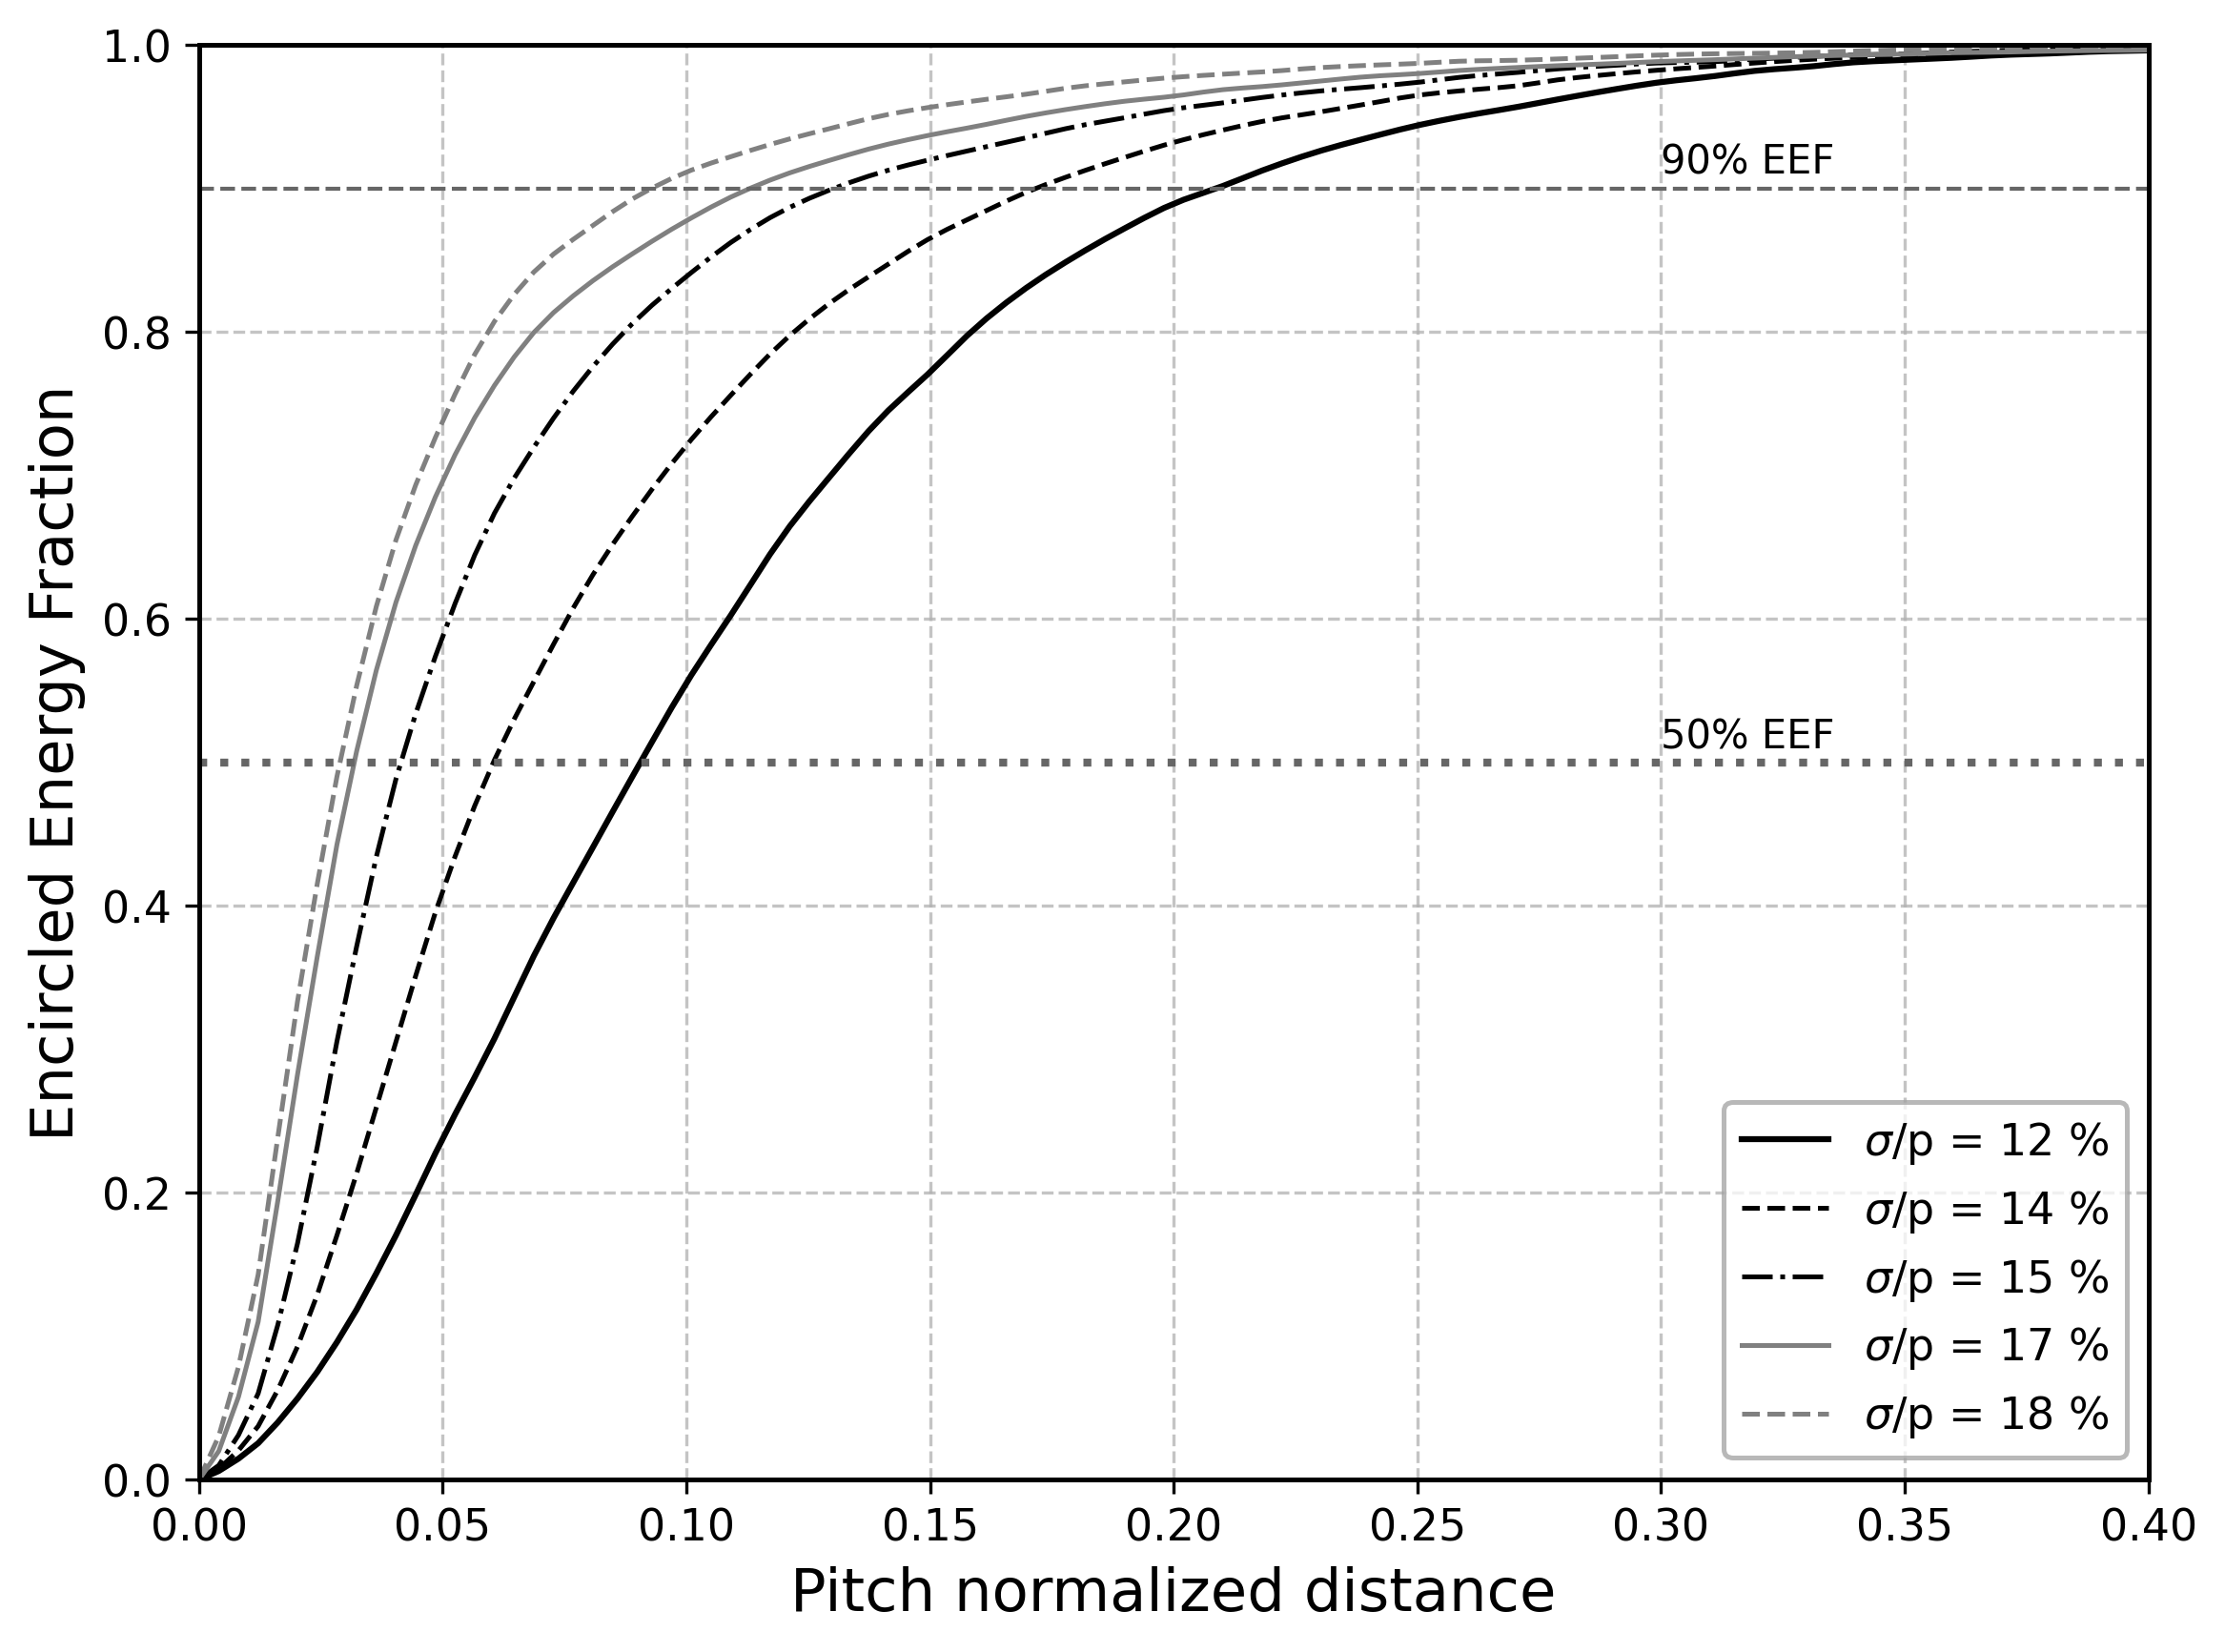
\includegraphics[width=0.7\linewidth]{figures/chapter4/position/eta_unmodeled_eef}
    \caption{Encircled energy fraction of the $\eta$ reconstruction algorithm for different values of the ratio between the diffused charge cloud and the pixel pitch as a function of the pitch normalized distance. The simulation is made with 20 ENC of noise.}
    \label{fig:eta_unmodeled_eef}
\end{figure}

%\begin{table}[htbp]
%\centering
%\begin{tabular}{c cccc}
%$\langle \sigma \rangle / p$ & EEF@50\% [pitch] & EEF@90\% [pitch]\\
%\midrule
%12.2 & 0.09 & 0.21 \\
%13.7 & 0.06 & 0.17 \\
%15.2 & 0.04 & 0.13 \\
%16.8 & 0.03 & 0.11 \\
%18.3 & 0.03 & 0.09 \\
%\bottomrule
%\end{tabular}
%\caption{Pitch distances at which EEF contains 50\% and 90\% of the events with the $\eta$ algorithm reconstruction, as a function of the ratio $\langle \sigma \rangle / p$. The values are extracted from Fig. \ref{fig:eta_unmodeled_eef}}
%\label{tab:eef_eta_unmodeled}
%\end{table}

The strength of this method is that a Monte Carlo simulation is not necessary. However, in case it is available, a different formulation of the $\eta$ algorithm can be made using the true incident positions.  In this case it is required knowing the charge diffusion model, but contrary to the likelihood method there are some approximations that can be made, making possible to solve analytically the problem. 

In the case of two-pixel events the position can only be reconstructed along the line connecting the two pixel centers, thus it is one-dimensional problem, as already seen above. Considering a photon which impacts on this line, the charge diffusion can be modeled as a one-dimensional Gaussian distribution centered on the incident point at a distance $r$ from the central pixel.

Given that the charge cloud dimension is small with respect to the pixel, all the charge is collected by these two pixels. As a consequence, the fraction of charge $\eta$ collected by the outer pixel, defined in Eq. \ref{eq:eta_2pix}, is a function of $r$ and can be calculated as the integral of the Gaussian

\begin{equation}
\eta(r) = \int ^{\infty}_{p/2} \frac{1}{\sqrt{2\pi}\sigma} \exp \left[ - \frac{(r' - r)^2}{2\sigma^2}  \right] dr' = \Phi \left( \frac{r - p/2}{\sigma} \right),
\label{eq:eta_2pix_int}
\end{equation}
where $\Phi(z)$ is the cumulative density function of the standard normal distribution and $p$ is the pixel pitch. Eq. \ref{eq:eta_2pix_int} can be inverted to find

\begin{equation}
r(\eta) = \frac{p}{2} + \sigma \Phi^{-1}(\eta),
\label{eq:eta_2pix_final}
\end{equation}
where $\Phi^{-1}(p)$ is the percent point function of the standard normal distribution.

The only unknown parameter in Eq. \ref{eq:eta_2pix_final} is $\sigma$, that could be estimated with Eq. \ref{eq:diff_sigma_dist}. However, this estimate would not take into account the presence of events occuring far from the axis, as shown in Fig. \ref{fig:2pix_scatter}. For this reason Monte Carlo simulations can be used to estimate the parameter.

To estimate $\sigma$ the projected distance $r$ of the Monte Carlo truth position onto the axis connecting the two pixel centers is calculated. A two-dimensional histogram is calculated using the resulting projected distance and $\eta$, as shown in Fig. \ref{fig:eta_2pix_r_distr}.

\begin{figure}[!b]
    \centering
    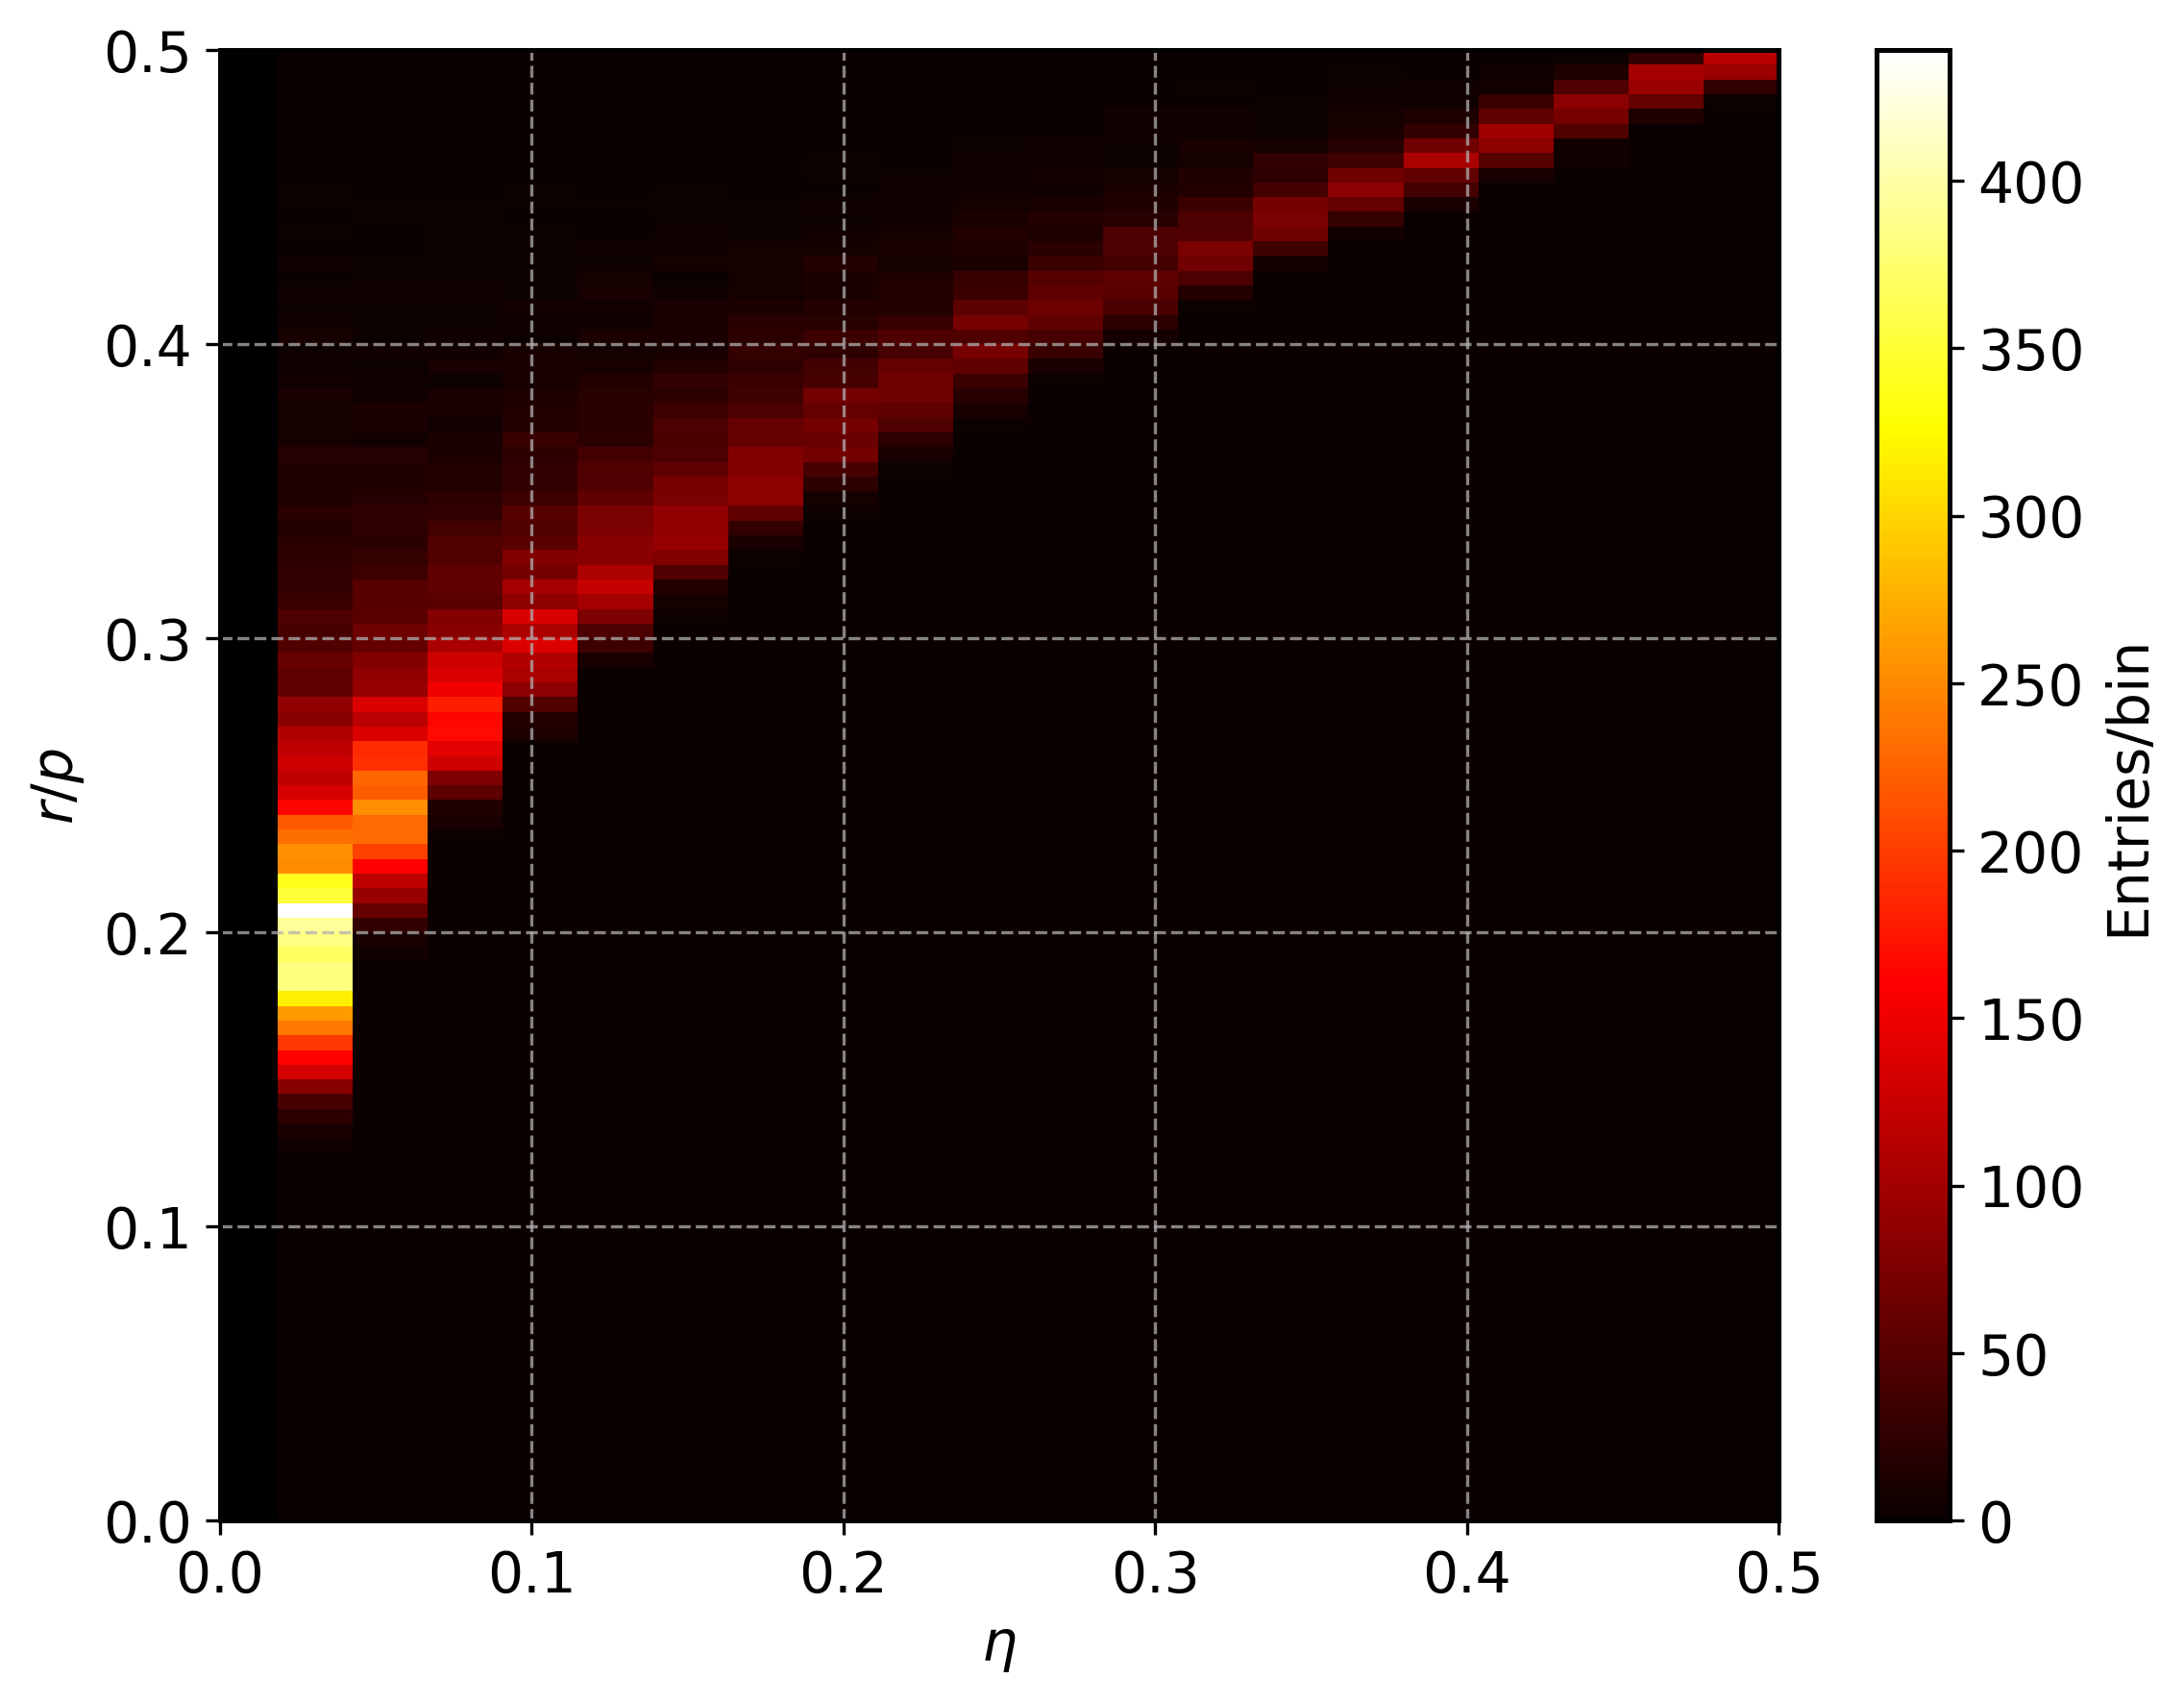
\includegraphics[width=0.49\linewidth]{figures/chapter4/position/eta_2pix_hist}
    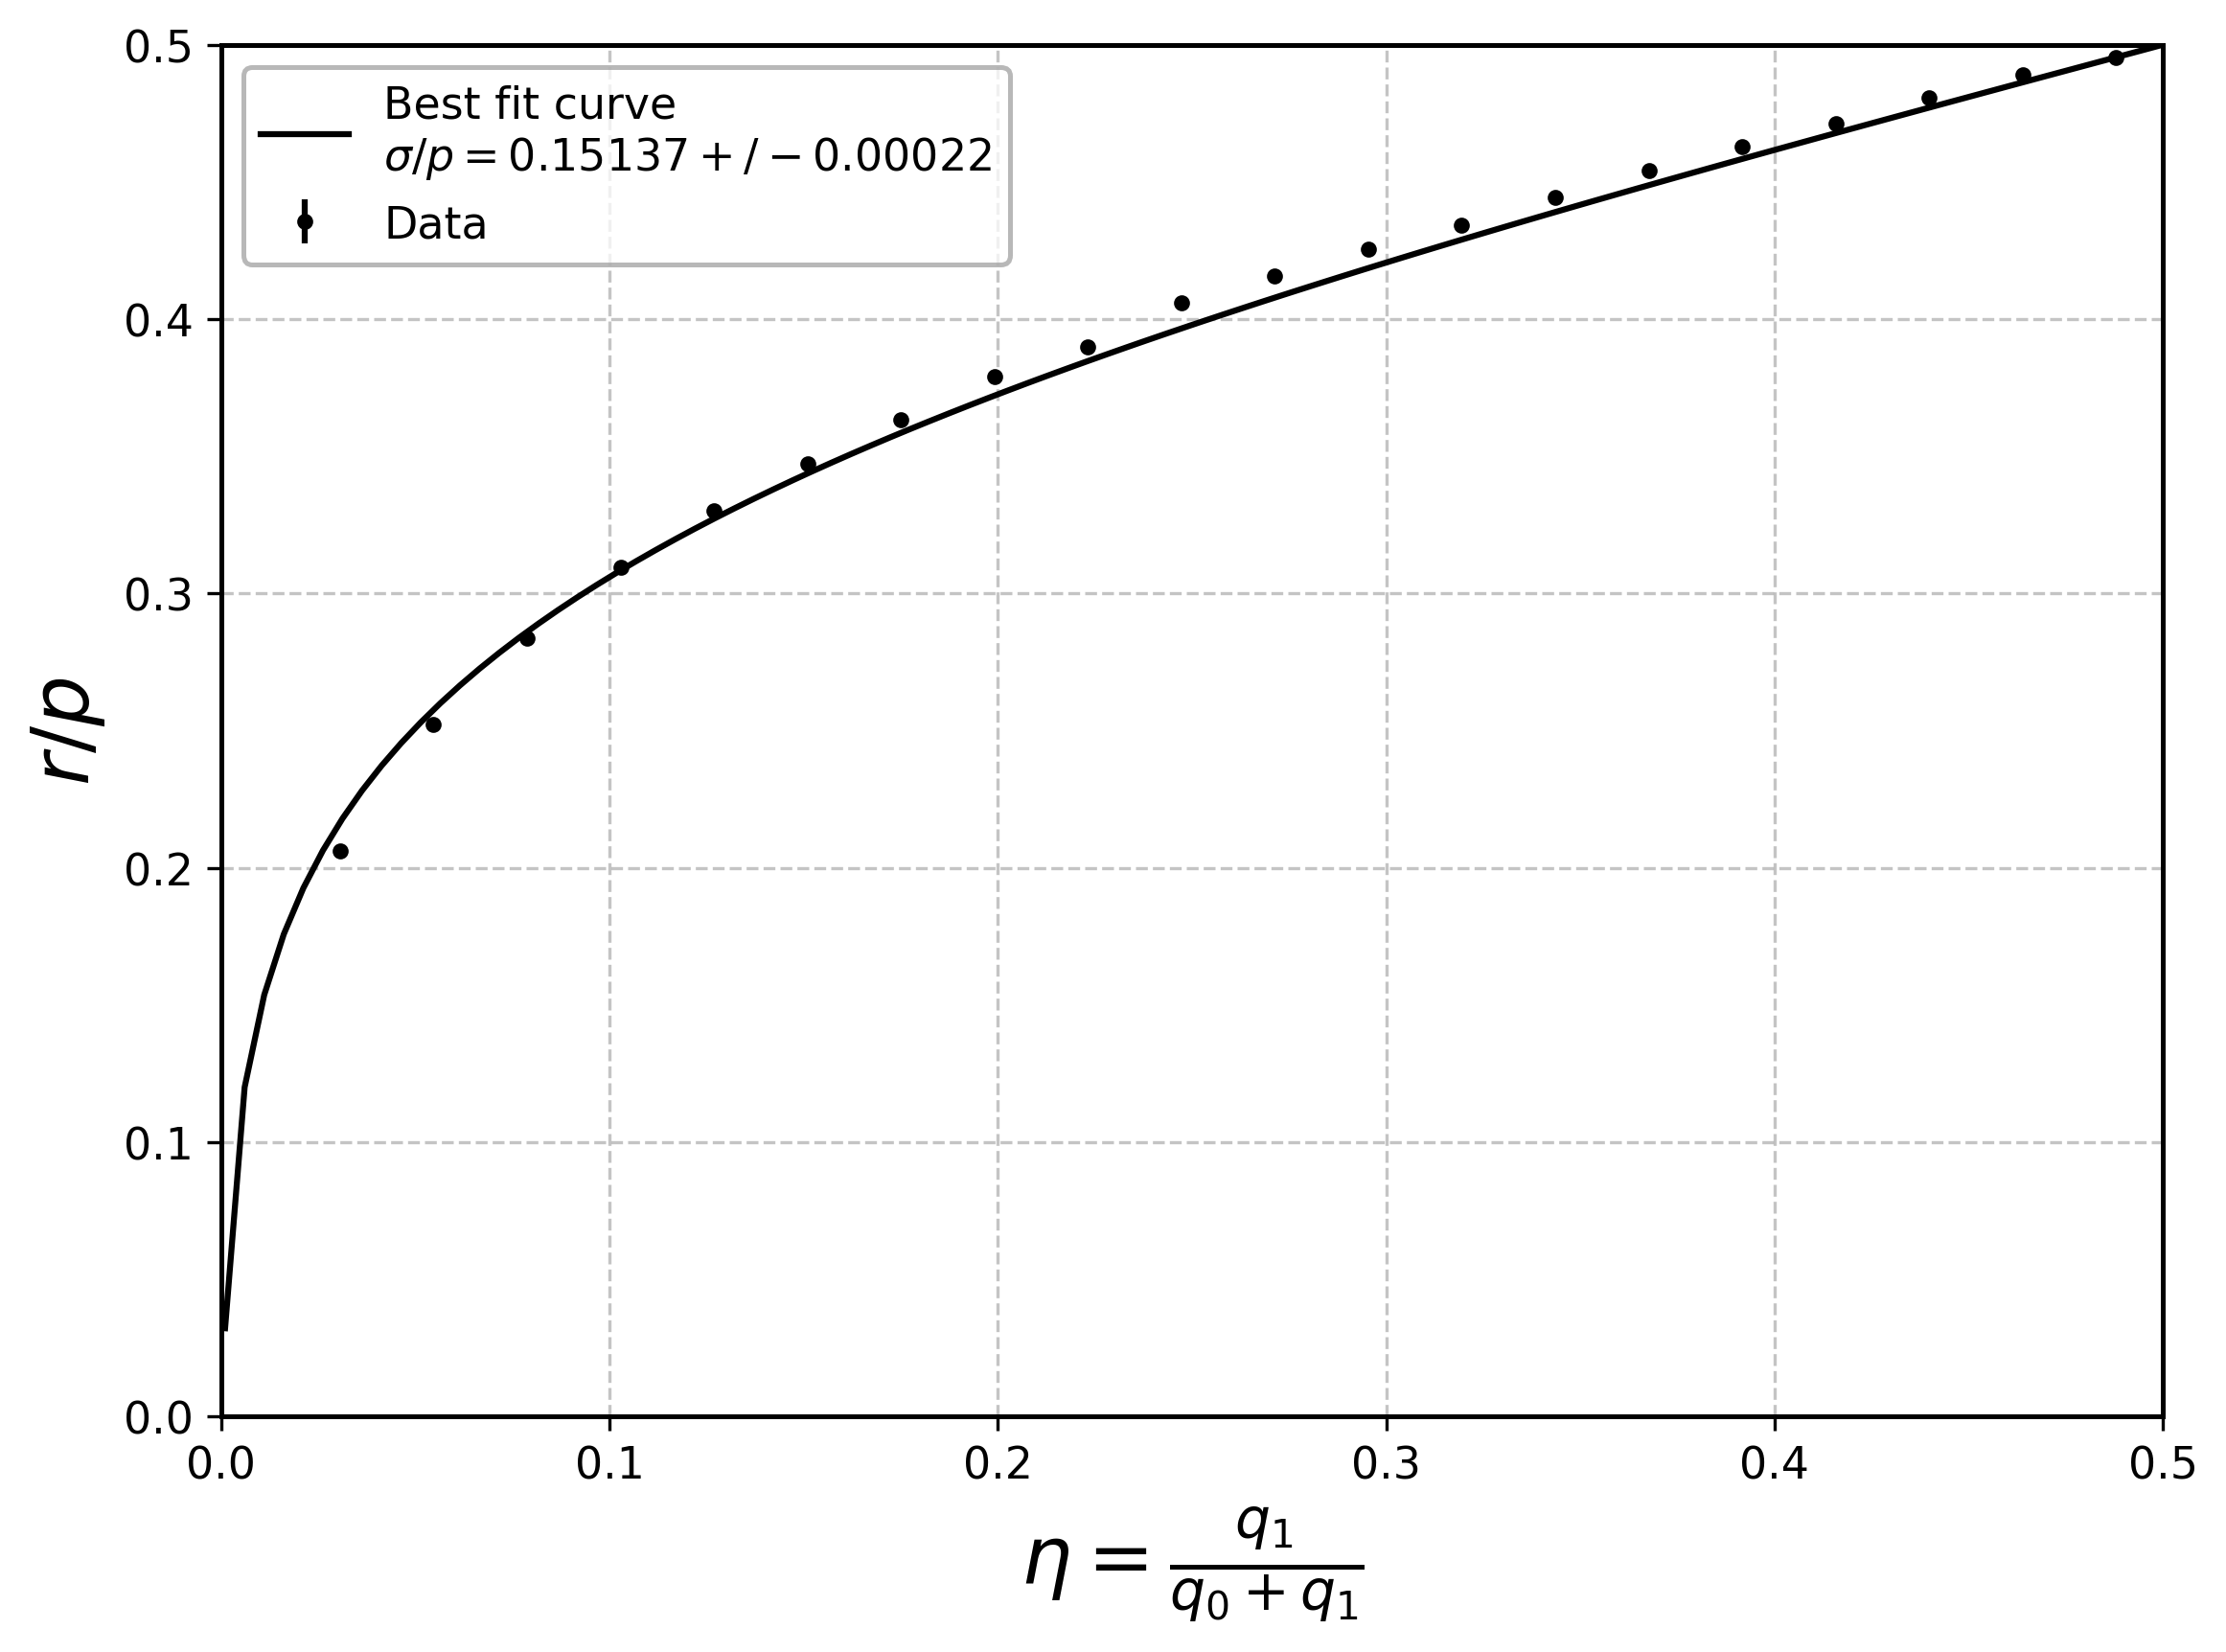
\includegraphics[width=0.49\linewidth]{figures/chapter4/position/eta_2pix_fit}
    \caption{Two-dimensional histogram showing the distribution of $r$ as a function of $\eta$ (left panel) and profile calculated from the latter, using the median of the $r$ distributions for each $\eta$ (right panel). The profile is fitted using Eq. \ref{eq:eta_2pix_final} as fit model to find the best-fit value of $\sigma$. The simulation has an estimated $\langle \sigma \rangle / p = 0.15$.}
    \label{fig:eta_2pix_r_distr}
\end{figure}

A profile of this histogram is then obtained by calculating the median of the $r$ distribution for each $\eta$ bins. The choice to use the median has been made because these distributions have long tails, thus the mean would not be the ideal location estimator.

The resulting profile is fitted using Eq. \ref{eq:eta_2pix_final} as fit model, with $\sigma$ being the only free parameter. The profile and the corresponding fit are shown in Fig. \ref{fig:eta_2pix_r_distr}.

A similar approach can be used for three-pixels events. As already said above, this case requires to separate between the radial and the angular coordinates into two independent one-dimensional two-pixel problems.

The idea behind this model is the same already discussed for the unmodeled $\eta$ algorithm. The radial component can be described by the $\eta_+$ variable, considering the two outer pixels as a single one with total charge given by the sum of the two. The problem is reduced to the same of two-pixel events, with the only difference being in the lower integration limit, which now is the distance of the vertex from the center. $\eta_+$ is given by

\begin{equation}
\eta_+(r) = \int ^{\infty}_{p/\sqrt{3}} \frac{1}{\sqrt{2\pi}\sigma} \exp \left[ - \frac{(r' - r)^2}{2\sigma^2}  \right] dr' = \Phi \left( \frac{r - p/\sqrt{3}}{\sigma} \right),
\label{eq:eta_3pix_int}
\end{equation}
which leads to

\begin{equation}
r(\eta_+) = \frac{p}{\sqrt{3}} + \sigma \Phi^{-1}(\eta_+).
\label{eq:eta_3pix_no_final}
\end{equation}

\begin{figure}[!b]
    \centering
    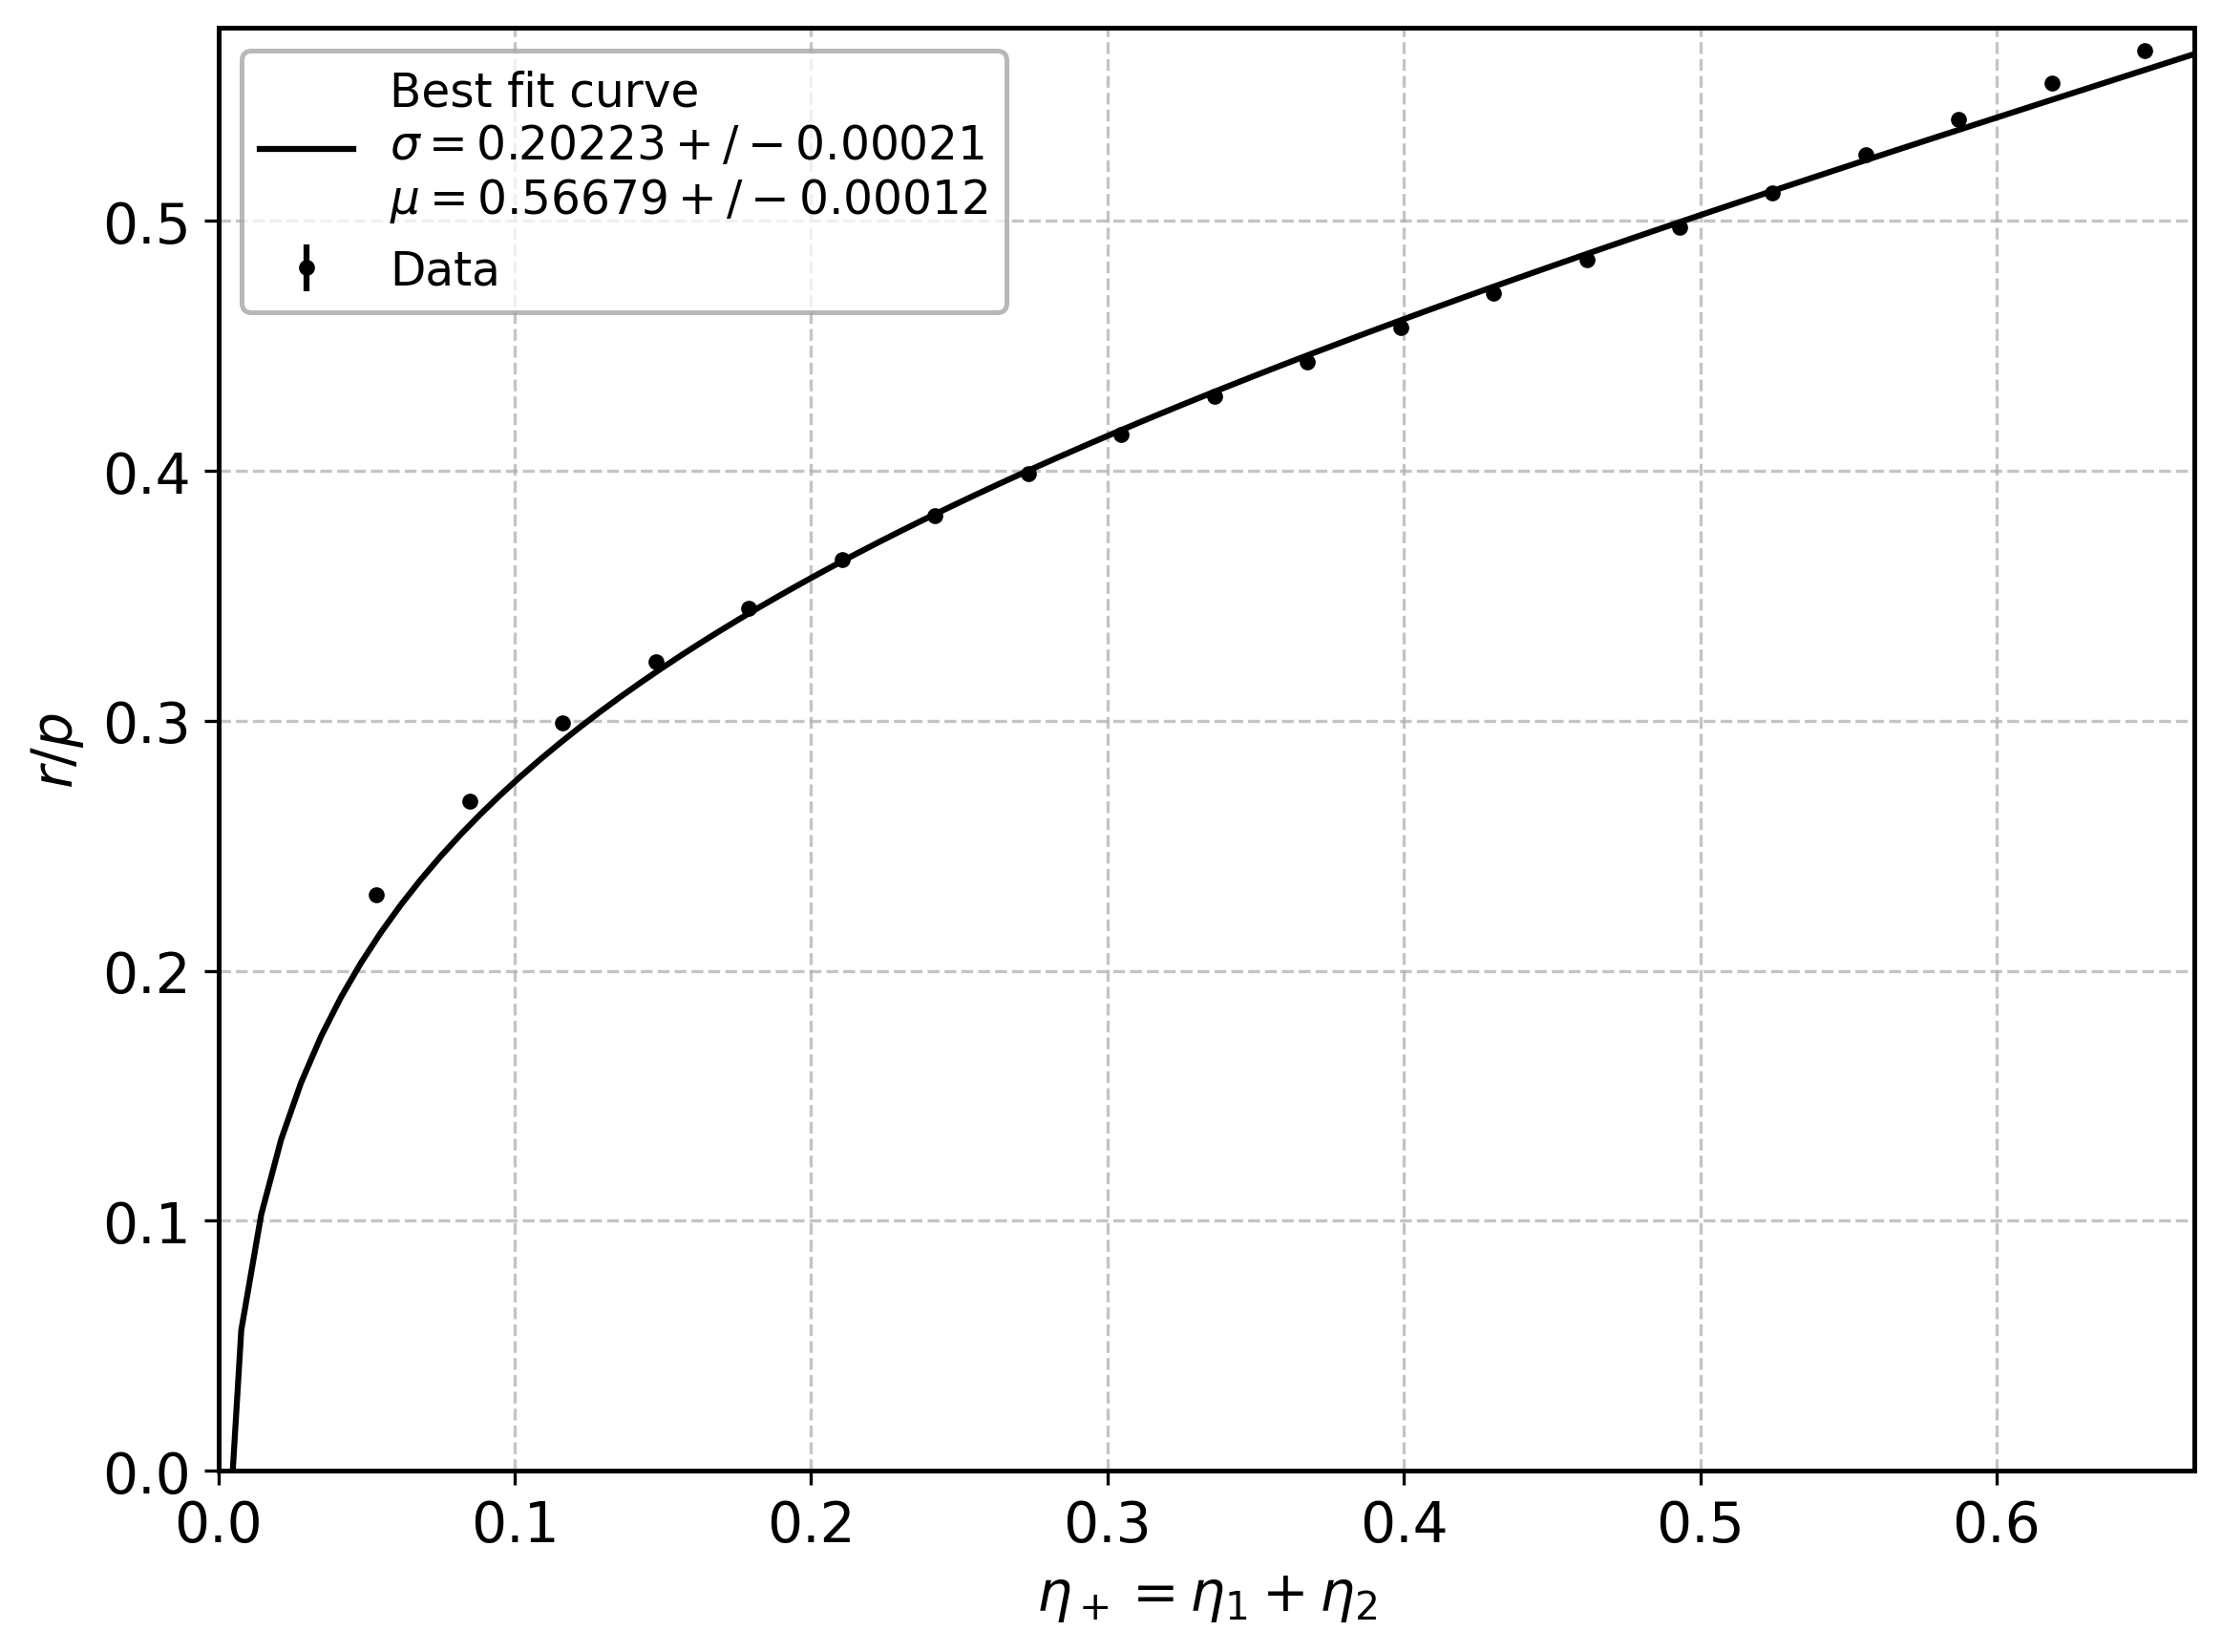
\includegraphics[width=0.49\linewidth]{figures/chapter4/position/eta_3pix_radial_fit}
    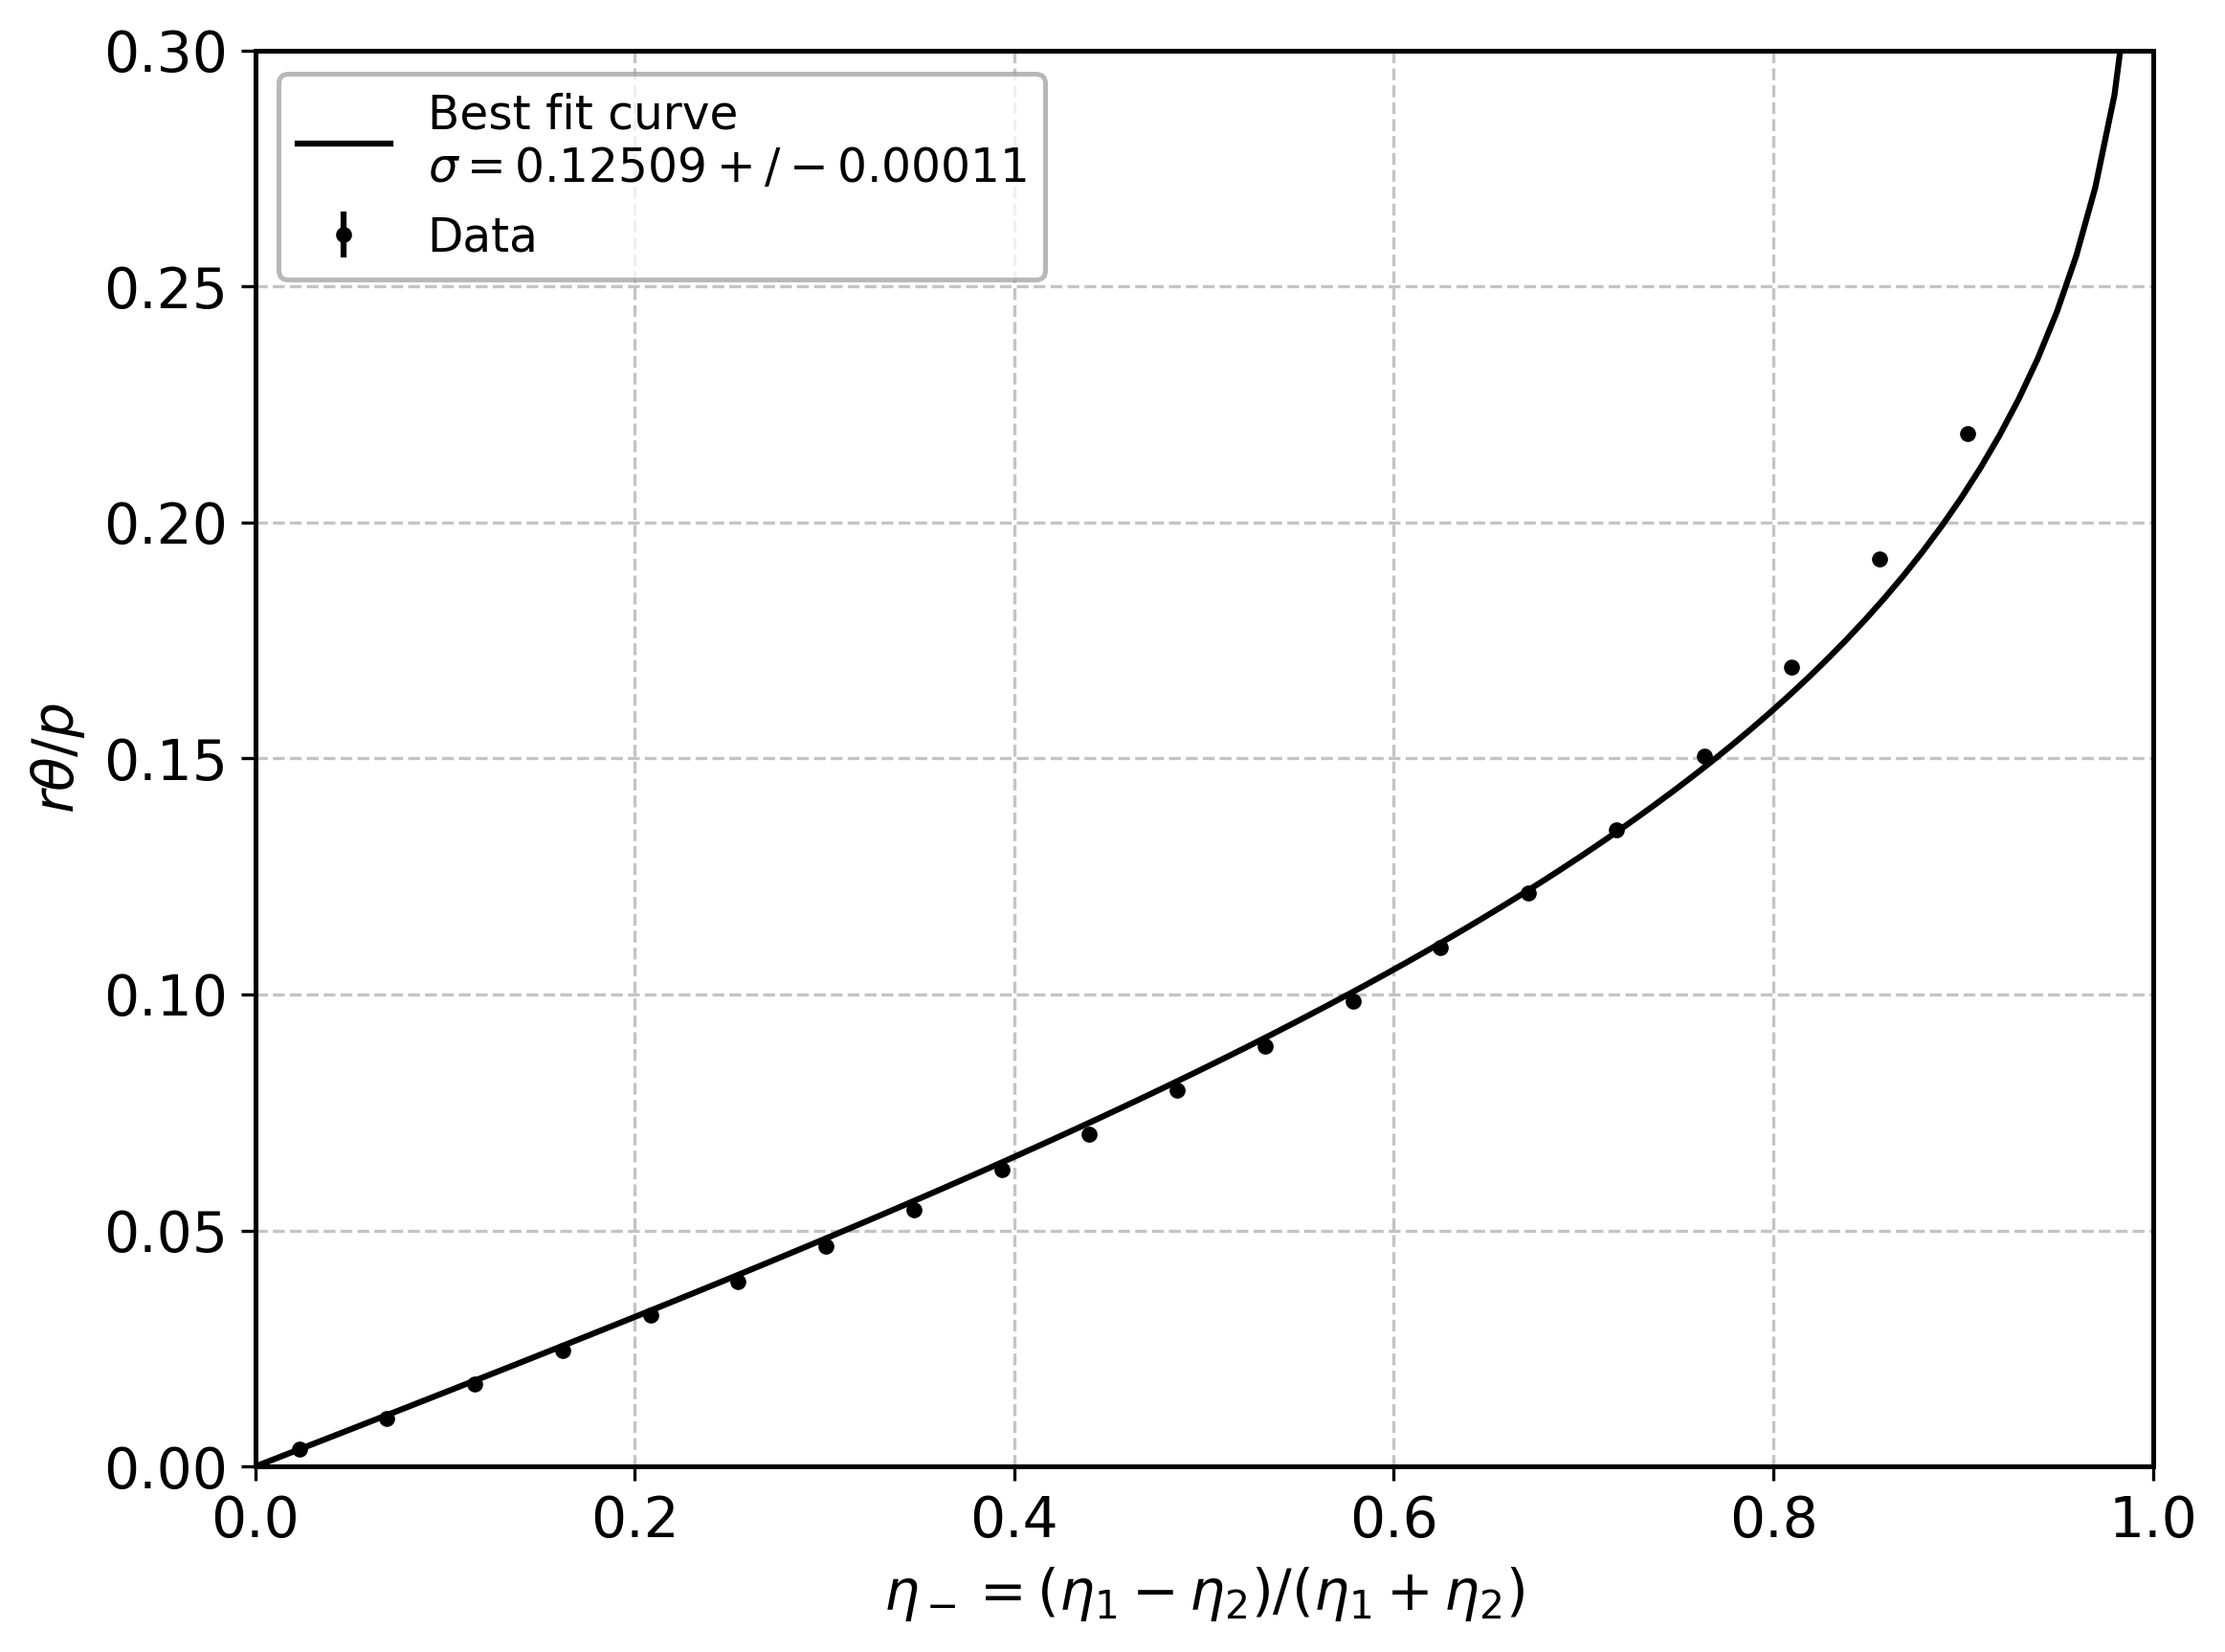
\includegraphics[width=0.49\linewidth]{figures/chapter4/position/eta_3pix_angular_fit}
    \caption{Profile and best-fit curves for the radial and angular components using Eqs. \ref{eq:eta_3pix_final} and \ref{eq:eta_3pix_ang_final}. The simulation has an estimated $\langle \sigma \rangle / p = 0.15$.}
    \label{fig:eta_3pix_fit}
\end{figure}

A small correction needs to be applied because Eq. \ref{eq:eta_3pix_no_final} does not take into account the hexagonal geometry of the pixels and that the internal angles of the hexagons are 120 degrees. Indeed, if a photon hits the vertex and the charge is equally divided between the three pixels, $\eta_+ = 2/3$ but $\Phi^{-1}(2/3) \neq 0$. As a consequence the impact point would not be reconstructed on the vertex, but outside the central pixel. The solution is to normalize $\eta_+$ in order to satisfy $r(2/3) = 1/\sqrt{3}$, thus the final model is
\begin{equation}
r(\eta_+) = \frac{p}{\sqrt{3}} + \sigma \Phi^{-1}\left( \frac{3}{4}\eta_+ \right).
\label{eq:eta_3pix_final}
\end{equation}

To find the model for the angular coordinate it is possible to consider only the two outer pixels, because $\eta_-$ is normalized with respect to the charge collected by these two pixels. The charge diffusion between these two pixels can be modeled as a one-dimensional Gaussian distribution centered in $y$, which is the distance from the midpoint of the pixels.

The relation between $\eta_-$ and $y$ can be found by calculating the fraction of Gaussian that falls inside each pixel, and is given by

\begin{equation}
\eta_-(y) = \frac{\eta_1}{\eta_+} - \frac{\eta_2}{\eta_+} = \left[1 - \Phi \left( - \frac{y}{\sigma} \right ) \right] - \Phi \left( - \frac{y}{\sigma} \right).
\label{eq:eta_3pix_ang}
\end{equation}
Using the approximation of small angles, the relation between the angular coordinate $\theta$ and $y$ is $\theta = y / r$. Inverting Eq. \ref{eq:eta_3pix_ang}, it is possible to find the relation between $\theta$ and $\eta_-$

\begin{equation}
\theta(\eta_-) =  - \frac{\sigma}{r} \Phi^{-1} \left( \frac{1 - \eta_-}{2} \right) = \frac{\sigma}{r} \Phi^{-1} \left( \frac{1 + \eta_-}{2} \right),
\label{eq:eta_3pix_ang_final}
\end{equation}
where it has been used that $\Phi^{-1}(1 - z) = - \Phi^{-1}(z)$.

To calibrate the radial and angular coordinates the strategy is identical to the calibration of two-pixels events. The projection onto the $\hat{r}$ axis and the angle with respect to it are calculated from Monte Carlo truth data of three-pixels events, then are binned in $\eta_+$ and $\eta_-$, and the median of the respective distributions are calculated. The resulting data are fitted with the respective models in Eqs. \ref{eq:eta_3pix_final} and \ref{eq:eta_3pix_ang_final}. Data and best-fit curves are shown in Fig. \ref{fig:eta_3pix_fit}.

As can be observed from Figs. \ref{fig:eta_2pix_r_distr} and \ref{fig:eta_3pix_fit}, the models describe very well the data, and the shape of the profiles are compatible with the cumulative distributions in Figs. \ref{fig:eta_2pix} and \ref{fig:eta_3pix} obtained with the unmodeled $\eta$ algorithm. This validates both the unmodeled and modeled algorithms, which converge to very similar results.

\begin{figure}[!b]
    \centering
    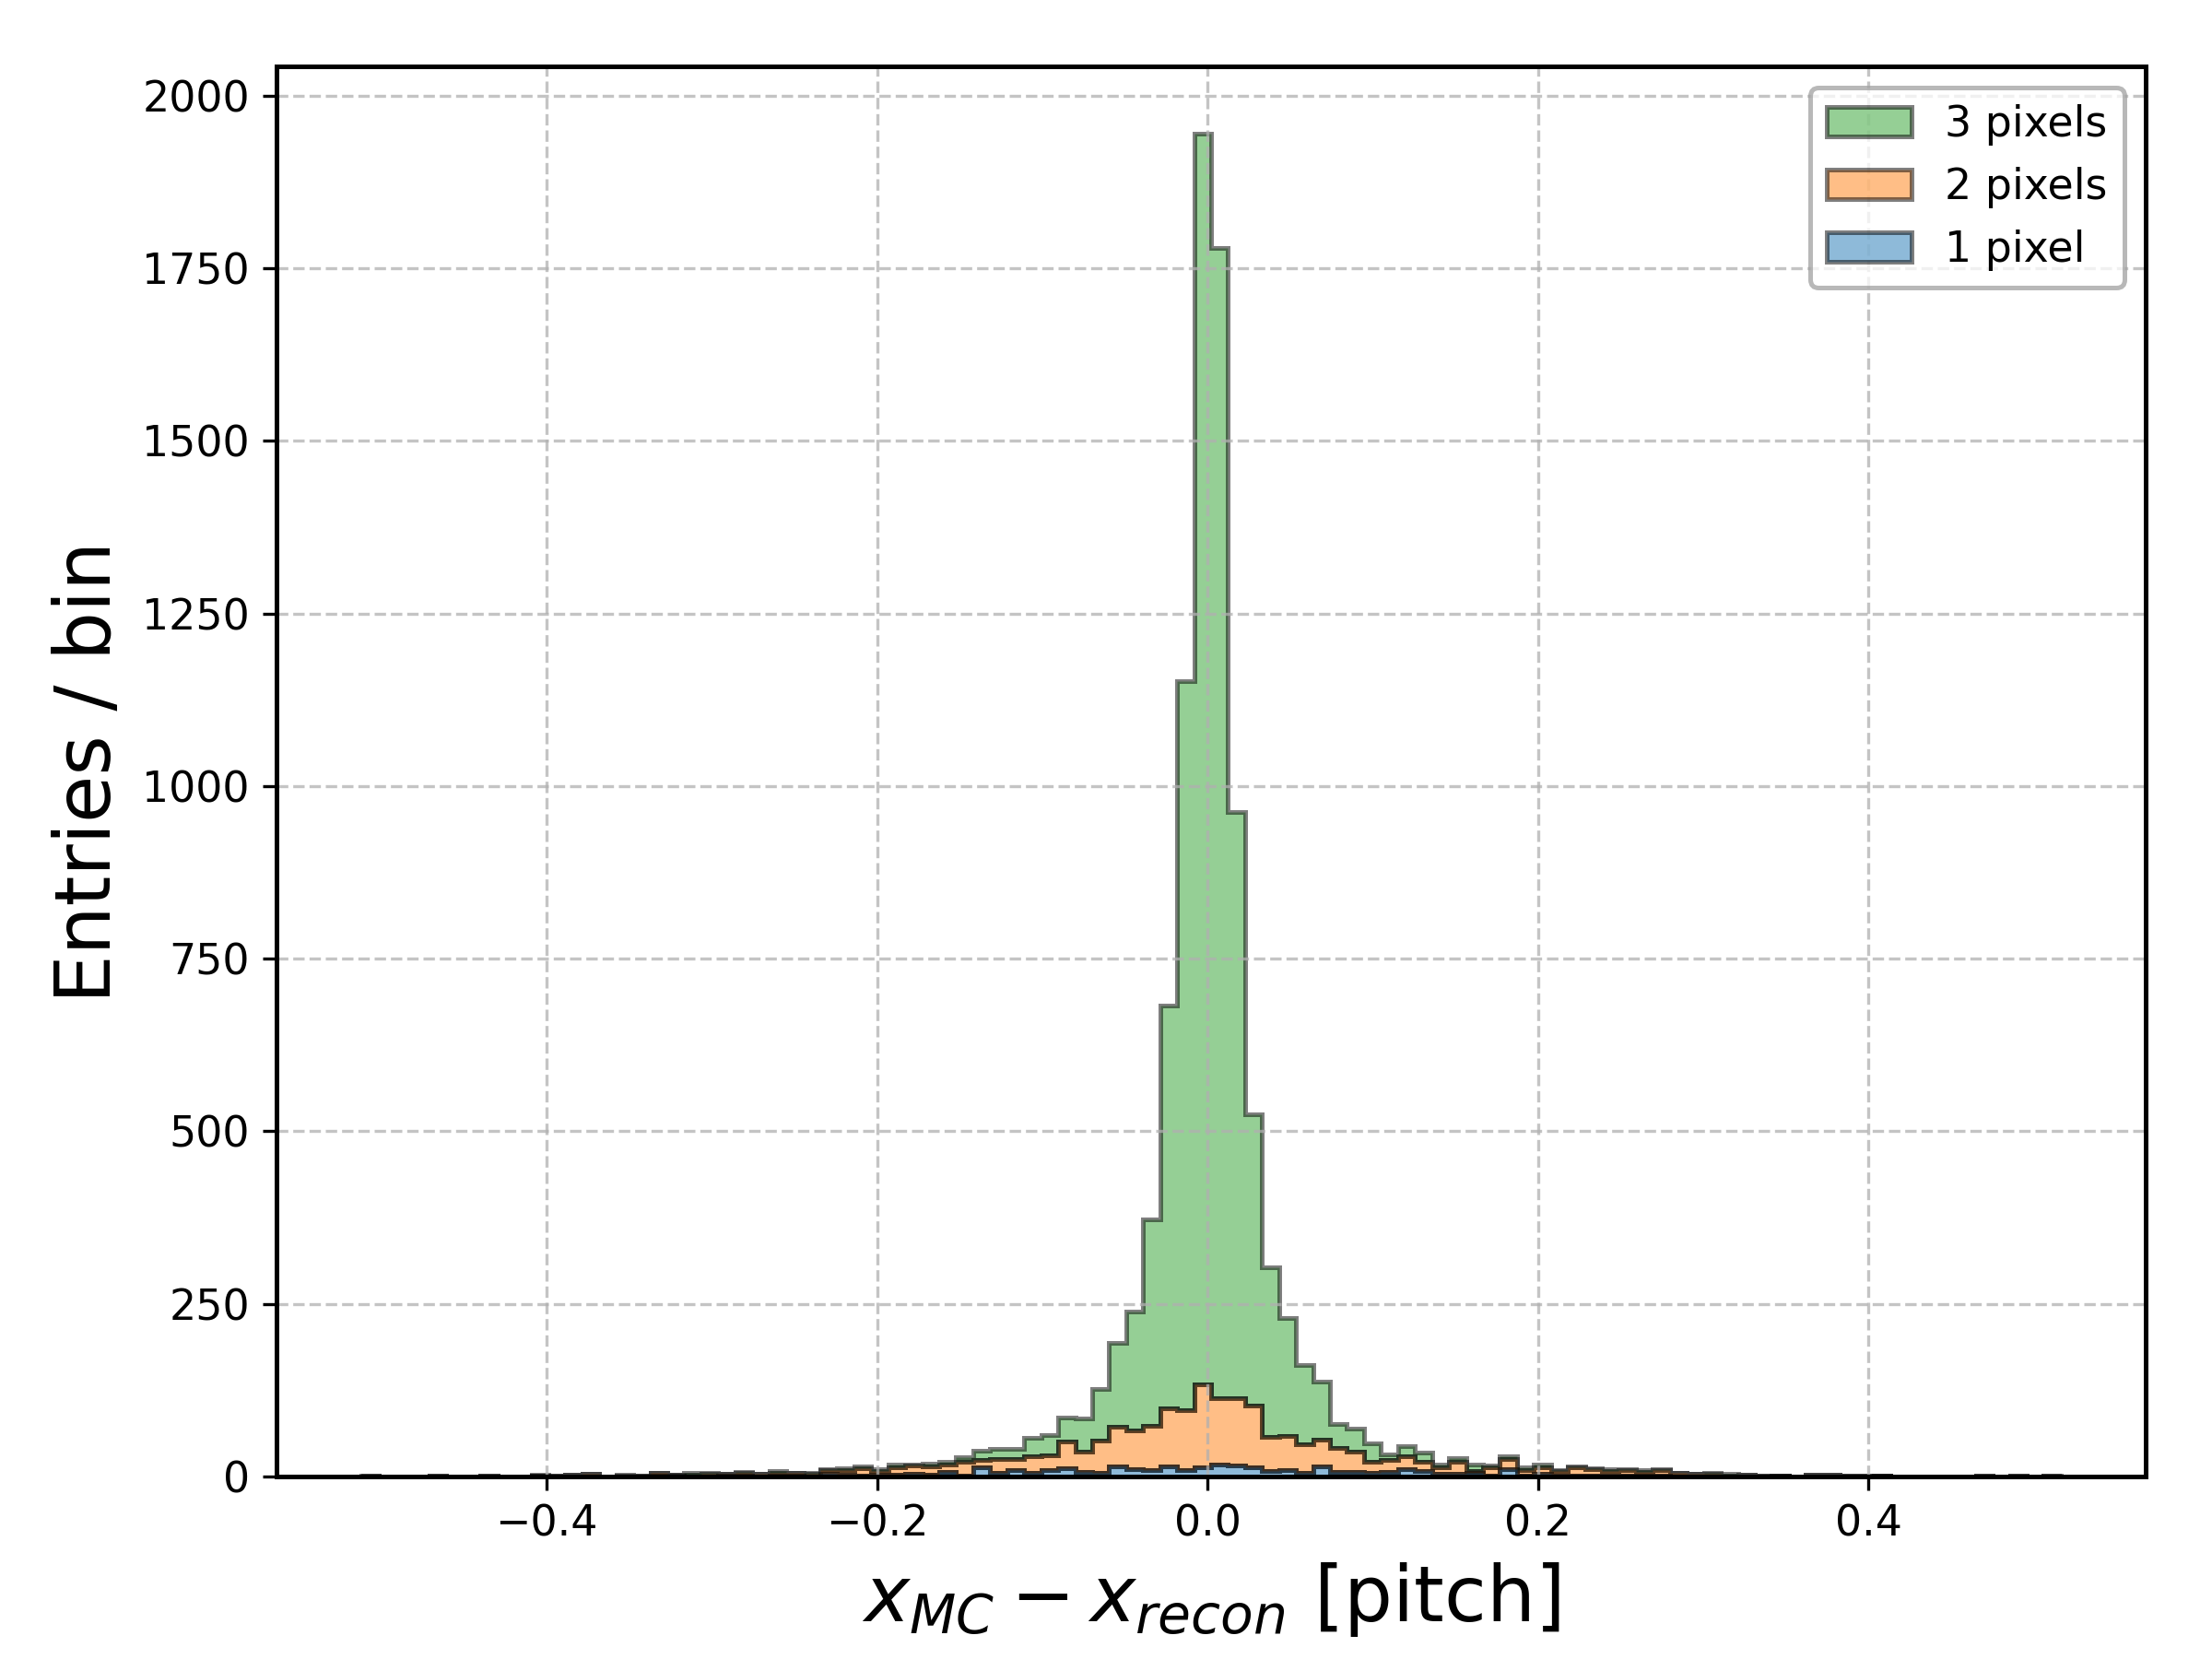
\includegraphics[width=0.49\linewidth]{figures/chapter4/position/eta_modeled_dx}
    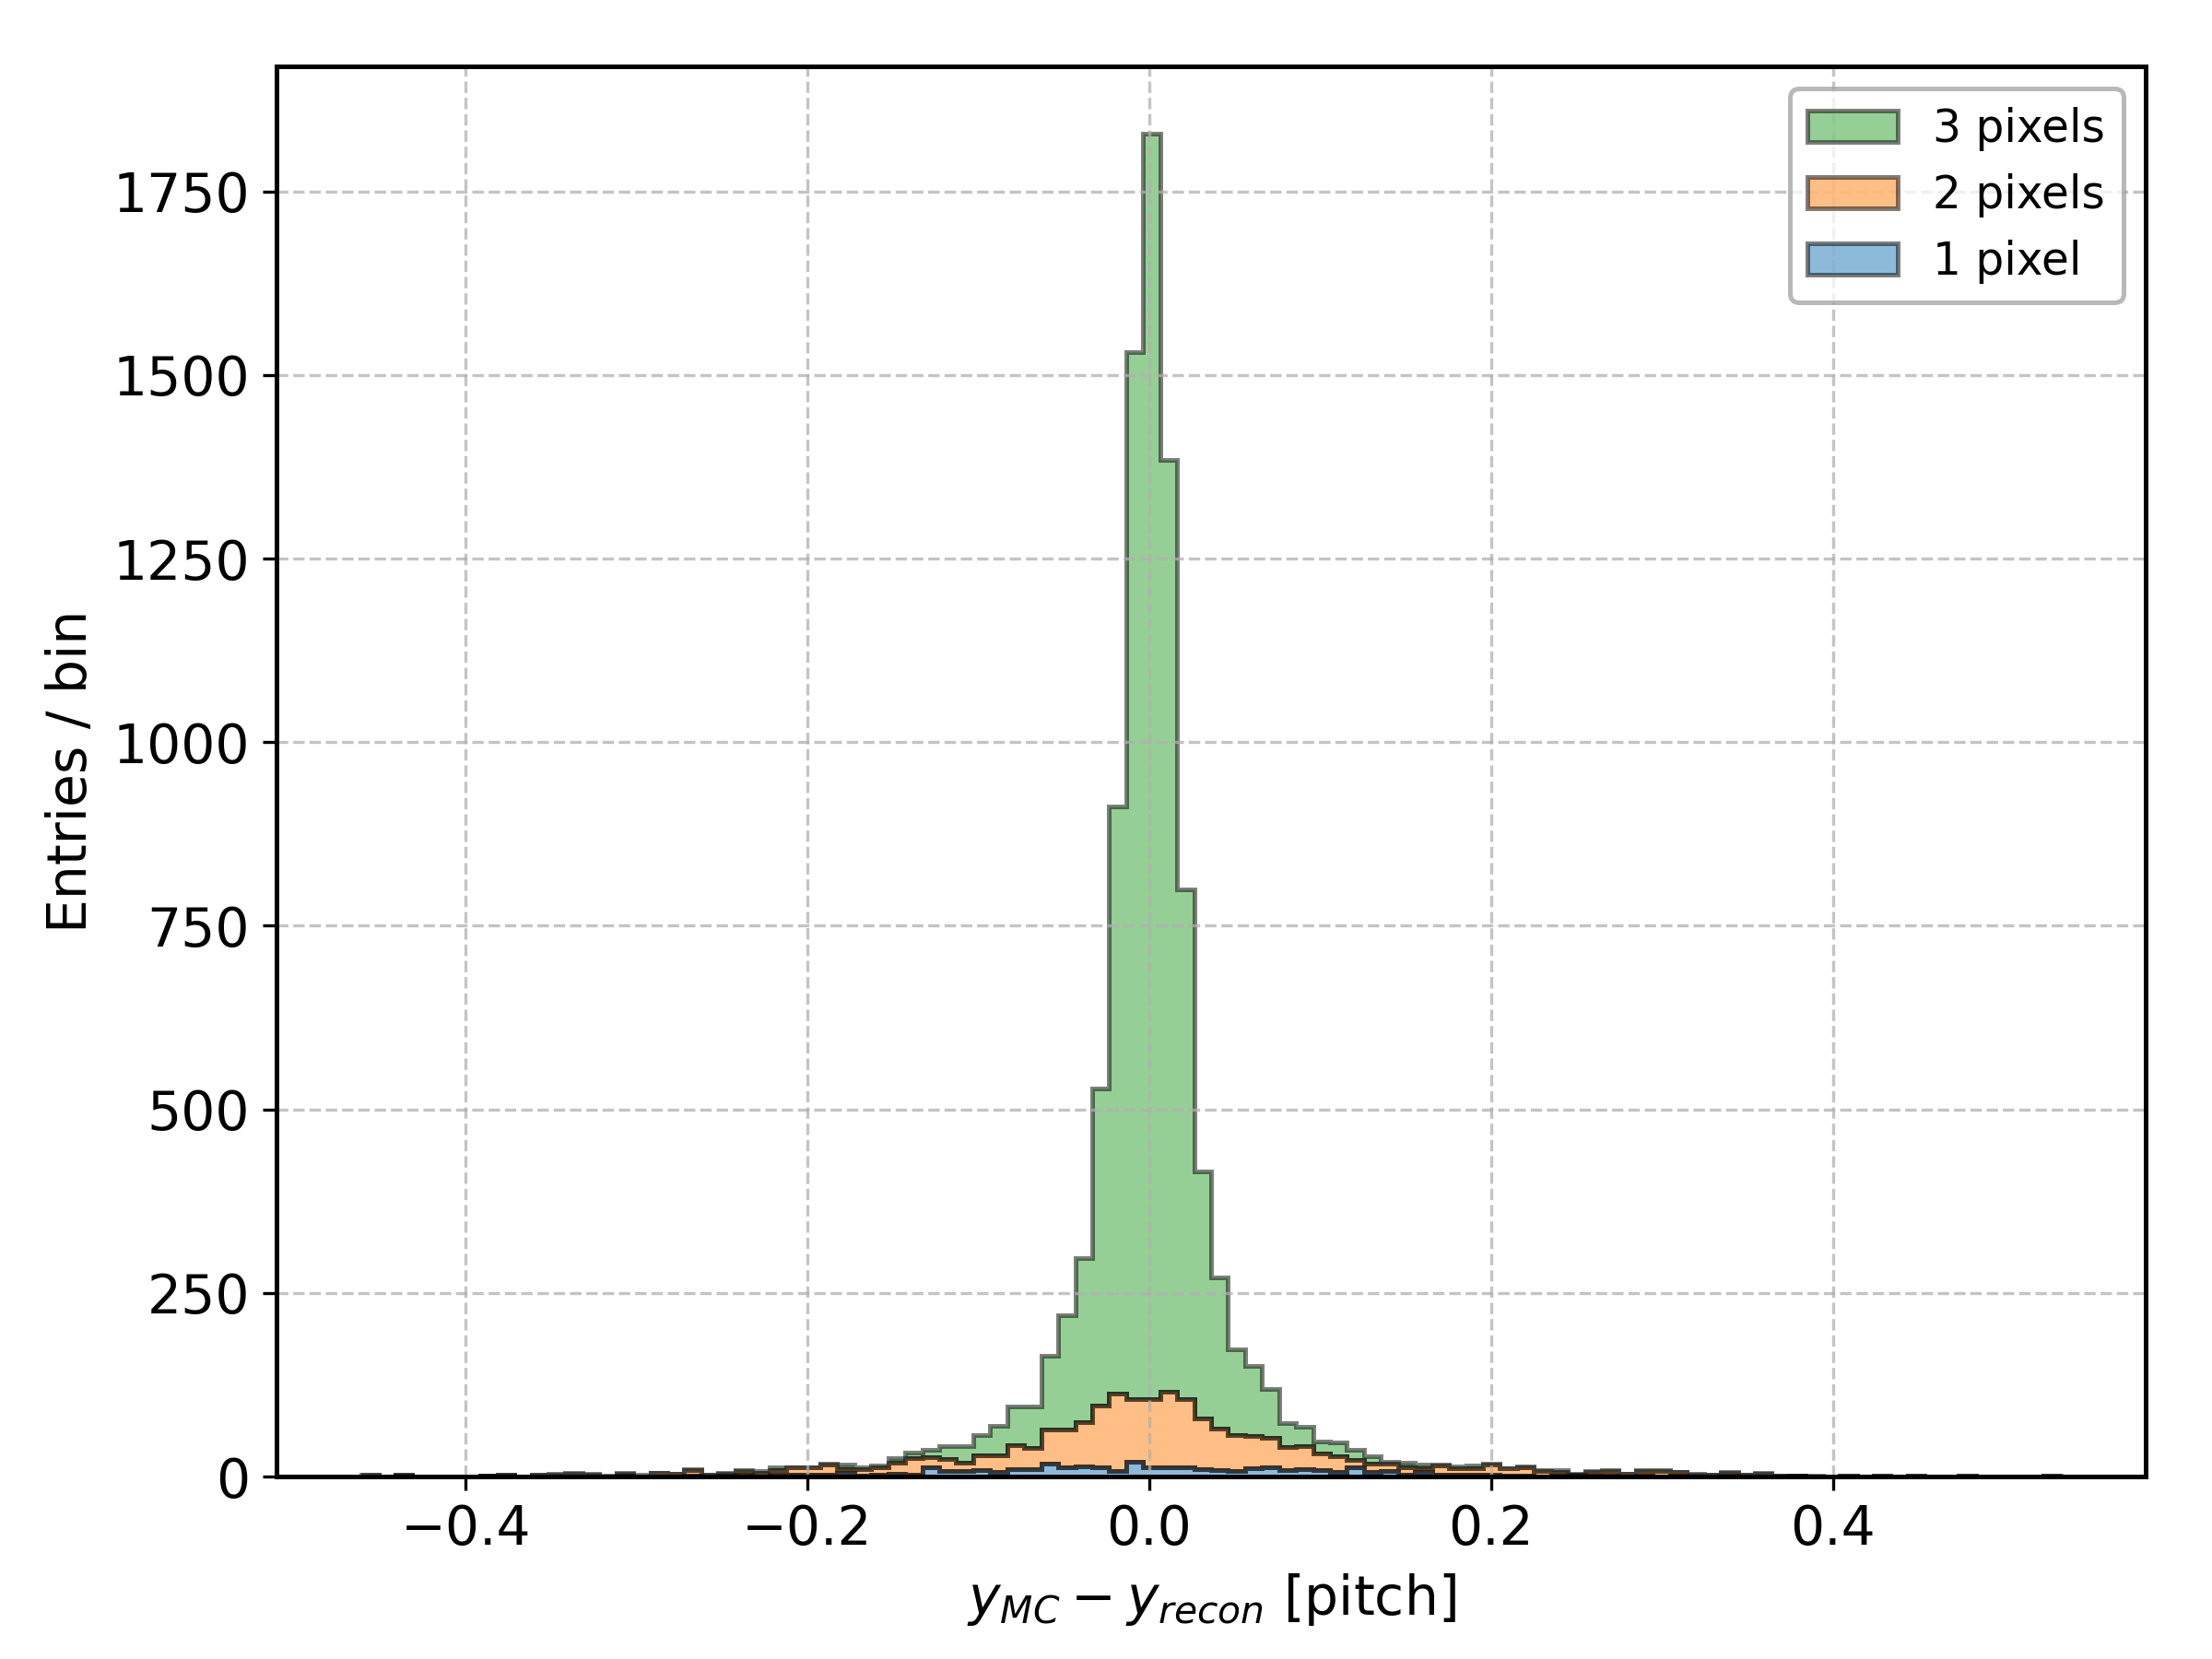
\includegraphics[width=0.49\linewidth]{figures/chapter4/position/eta_modeled_dy}
    \caption{Residuals distributions of the modeled eta algorithm for the $x$ and $y$ directions, calculated as the difference between the reconstructed and the Monte Carlo truth $x$ and $y$ components. The events are separated by cluster size, with each color representing a specific cluster size. The histograms are stacked on each other. The simulation is made with a 8 keV monochromatic source, 20 ENC of noise and ratio between the diffused charge cloud sigma and the pitch of 15\%.}
    \label{fig:eta_modeled_dx_dy}
\end{figure}

However, it can be noted that the best-fit values of $\sigma$ for the three fits are different. The simulation was performed with an average ratio $\langle \sigma \rangle / p = 0.15$, and only the parameter obtained from two-pixel events is compatible with the expected value. These discrepancies can be attributed to the spatial distribution of the events around the projection axes. Indeed, when this distribution is broad, as in the case of three-pixel events (Fig.~\ref{fig:3pix_scatter}), the deviation from the expected value is larger than for two-pixel events (Fig.~\ref{fig:2pix_scatter}). This must be taken into account, as calibration via Monte Carlo simulations becomes necessary, and the nominal value of $\langle \sigma \rangle /p$ estimated through Eqs. \ref{eq:z_average} and \ref{eq:diff_sigma_dist} cannot be directly used.

Once the best-fit parameters have been estimated from simulations, a separate dataset can be analyzed and the resulting residuals distributions are shown in Fig. \ref{fig:eta_modeled_dx_dy}. As for the other cases where the physics of charge diffusion has been taken into account, the resulting distributions are narrow and unimodal.

Moreover, the EEF of the modeled $\eta$ algorithm is very steep and has less relevant tails with respect to the MLE algorithm, as visible in Fig. \ref{fig:eta_modeled_eef}. As expected, the EEF becomes steeper for larger diffusion widths. 
%The distances at which the EEF contains 50\% and 90\% of the events are listed in Tab. \ref{tab:eta_modeled_eef}.

\begin{figure}[h]
    \centering
    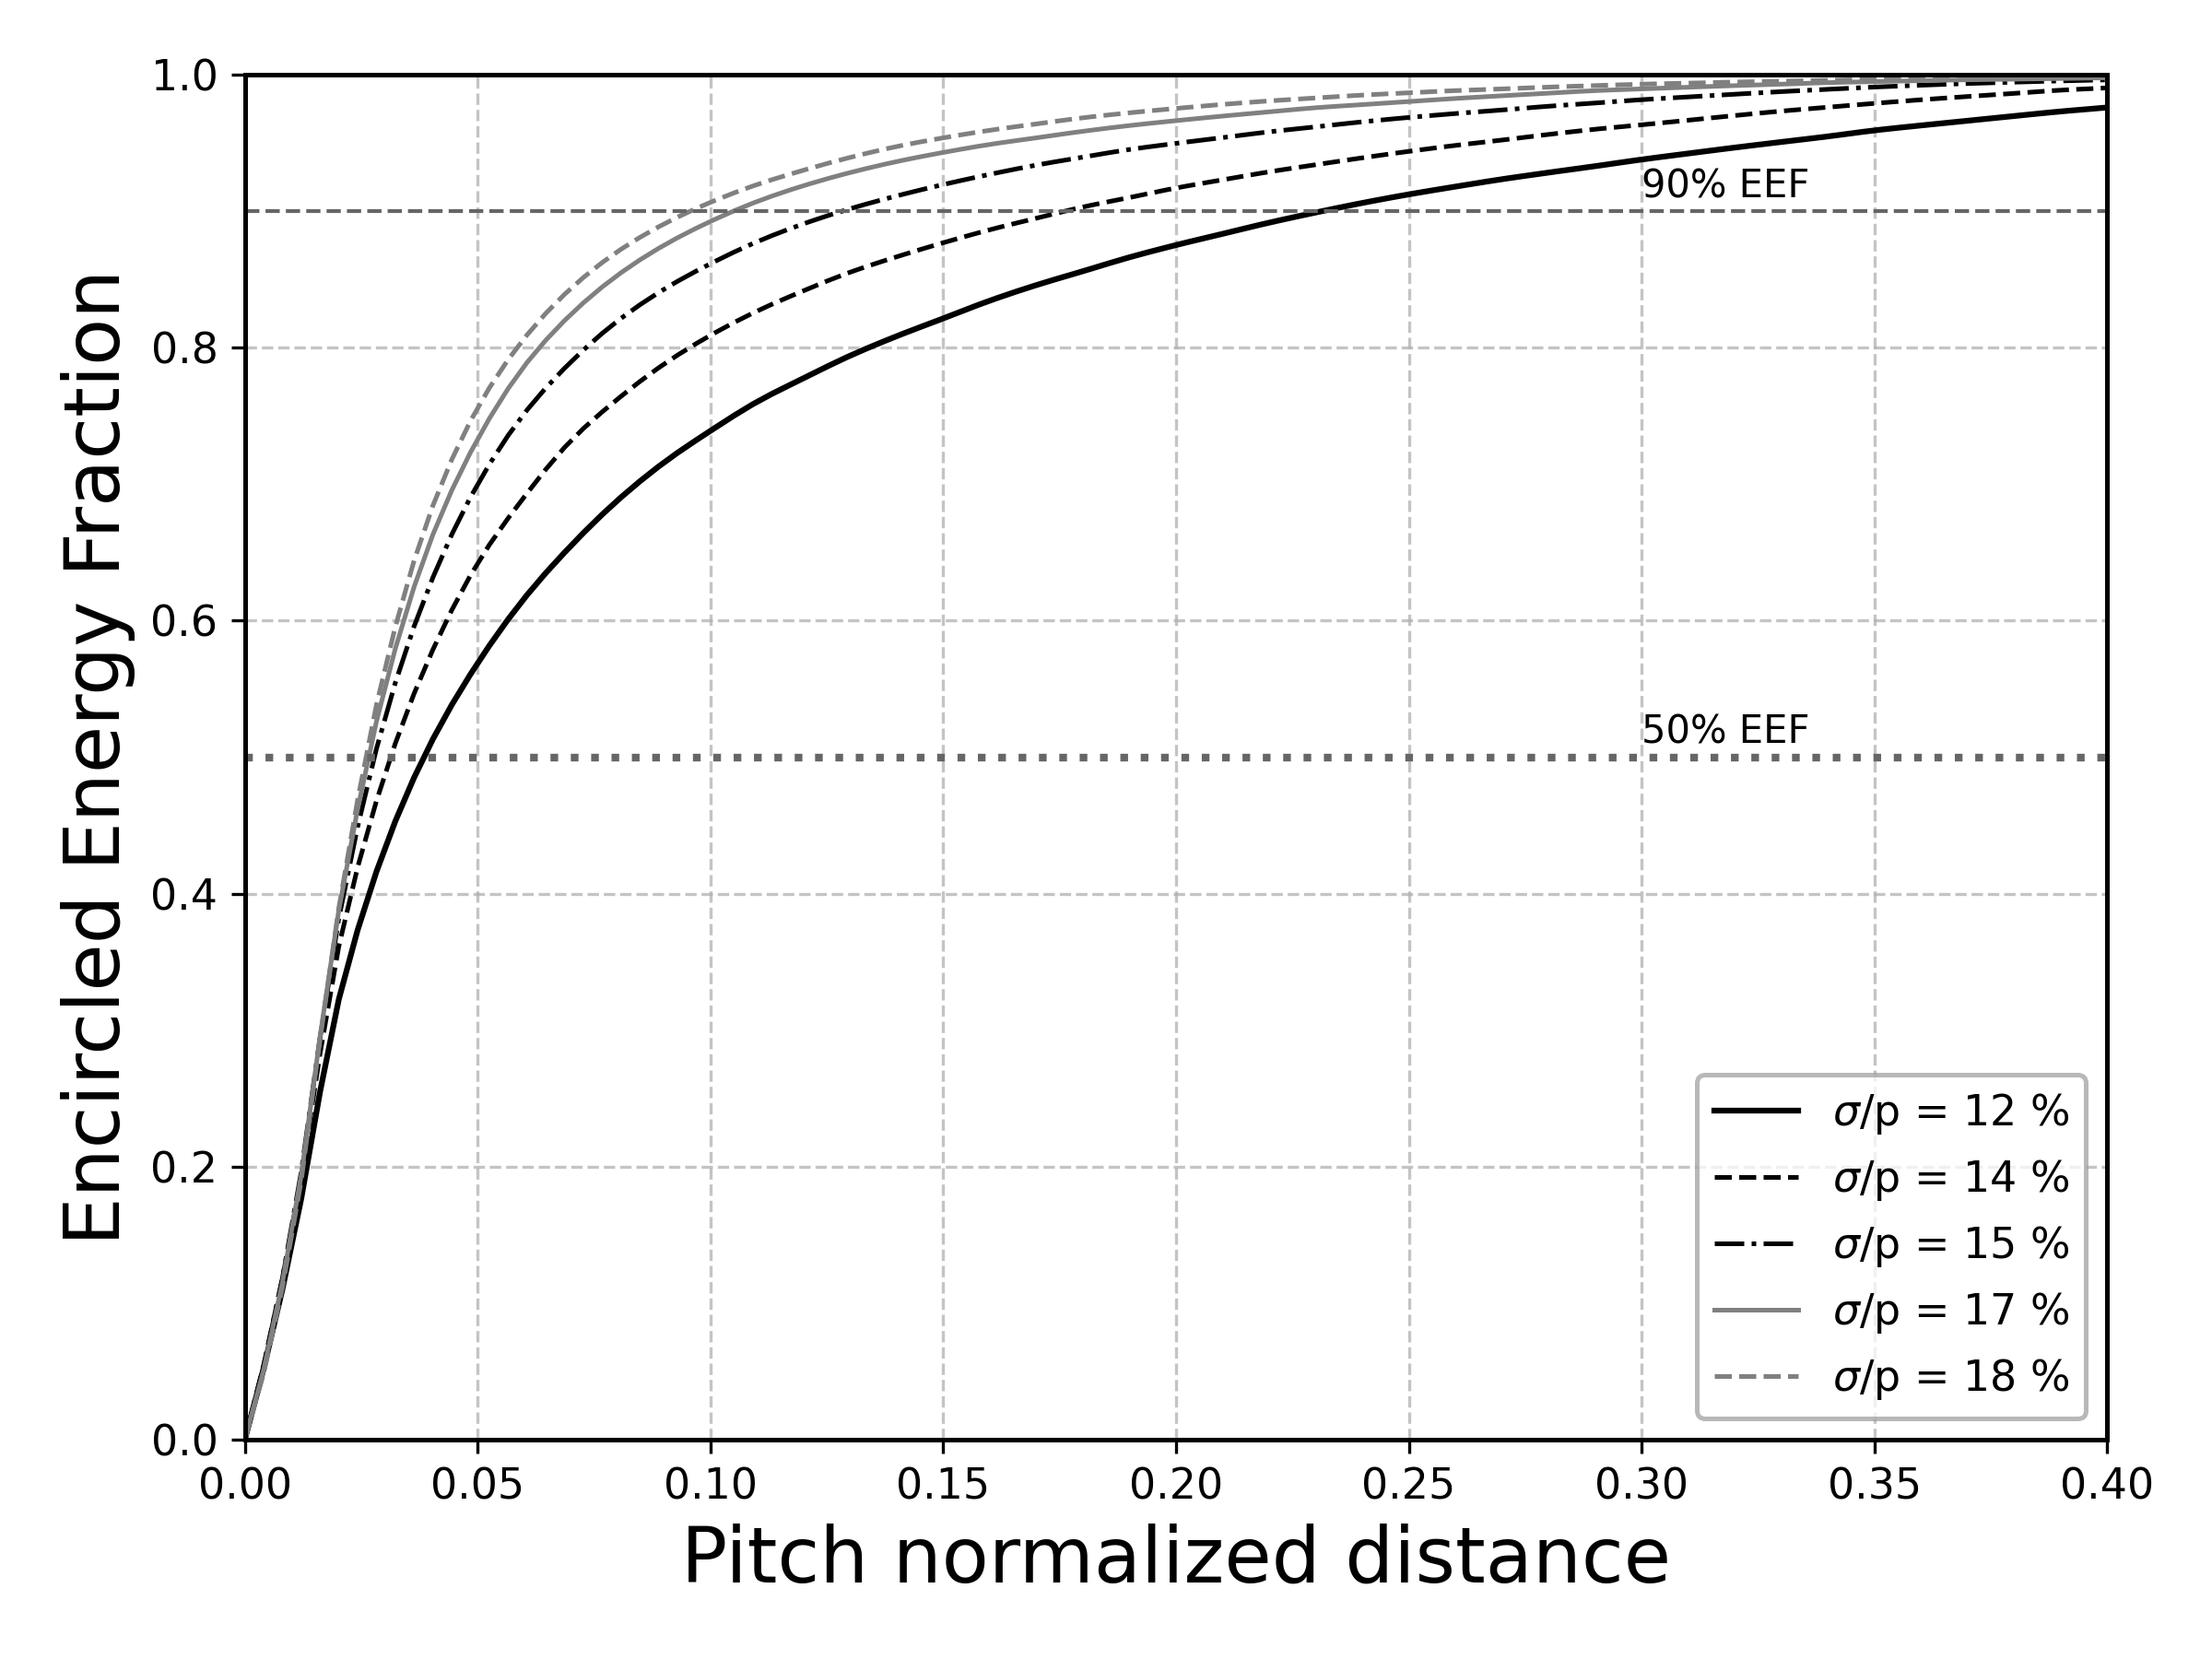
\includegraphics[width=0.7\linewidth]{figures/chapter4/position/eta_modeled_eef}
    \caption{Encircled energy fraction of the modeled eta reconstruction for different values of the ratio between the diffused charge cloud and the pixel pitch as a function of the pitch normalized distance. The simulation is made with 20 ENC of noise.}
    \label{fig:eta_modeled_eef}
\end{figure}

%\begin{table}[htbp]
%\centering
%\begin{tabular}{c cccc}
%$\langle \sigma \rangle / p$ & EEF@50\% [pitch] & EEF@90\% [pitch]\\
%\midrule
%12.2 & 0.04 & 0.23 \\
%13.7 & 0.03 & 0.18 \\
%15.2 & 0.03 & 0.13 \\
%16.8 & 0.03 & 0.11 \\
%18.3 & 0.03 & 0.10 \\
%\bottomrule
%\end{tabular}
%\caption{Pitch distances at which EEF contains 50\% and 90\% of the events with modeled eta reconstruction, as a function of the ratio $\langle \sigma \rangle / p$. The values are extracted from Fig. \ref{fig:eta_modeled_eef}}
%\label{tab:eta_modeled_eef}
%\end{table}

\subsection{Algorithms comparison}
\label{subsec:position_comparison}

To summarize and compare the results of the different reconstruction algorithms, Fig. \ref{fig:eef} shows the values of EEF@50\% and EEF@90\% as a function of the $\langle \sigma \rangle / p$ ratio for all the discussed methods.

\begin{figure}[htbp]
    \centering
    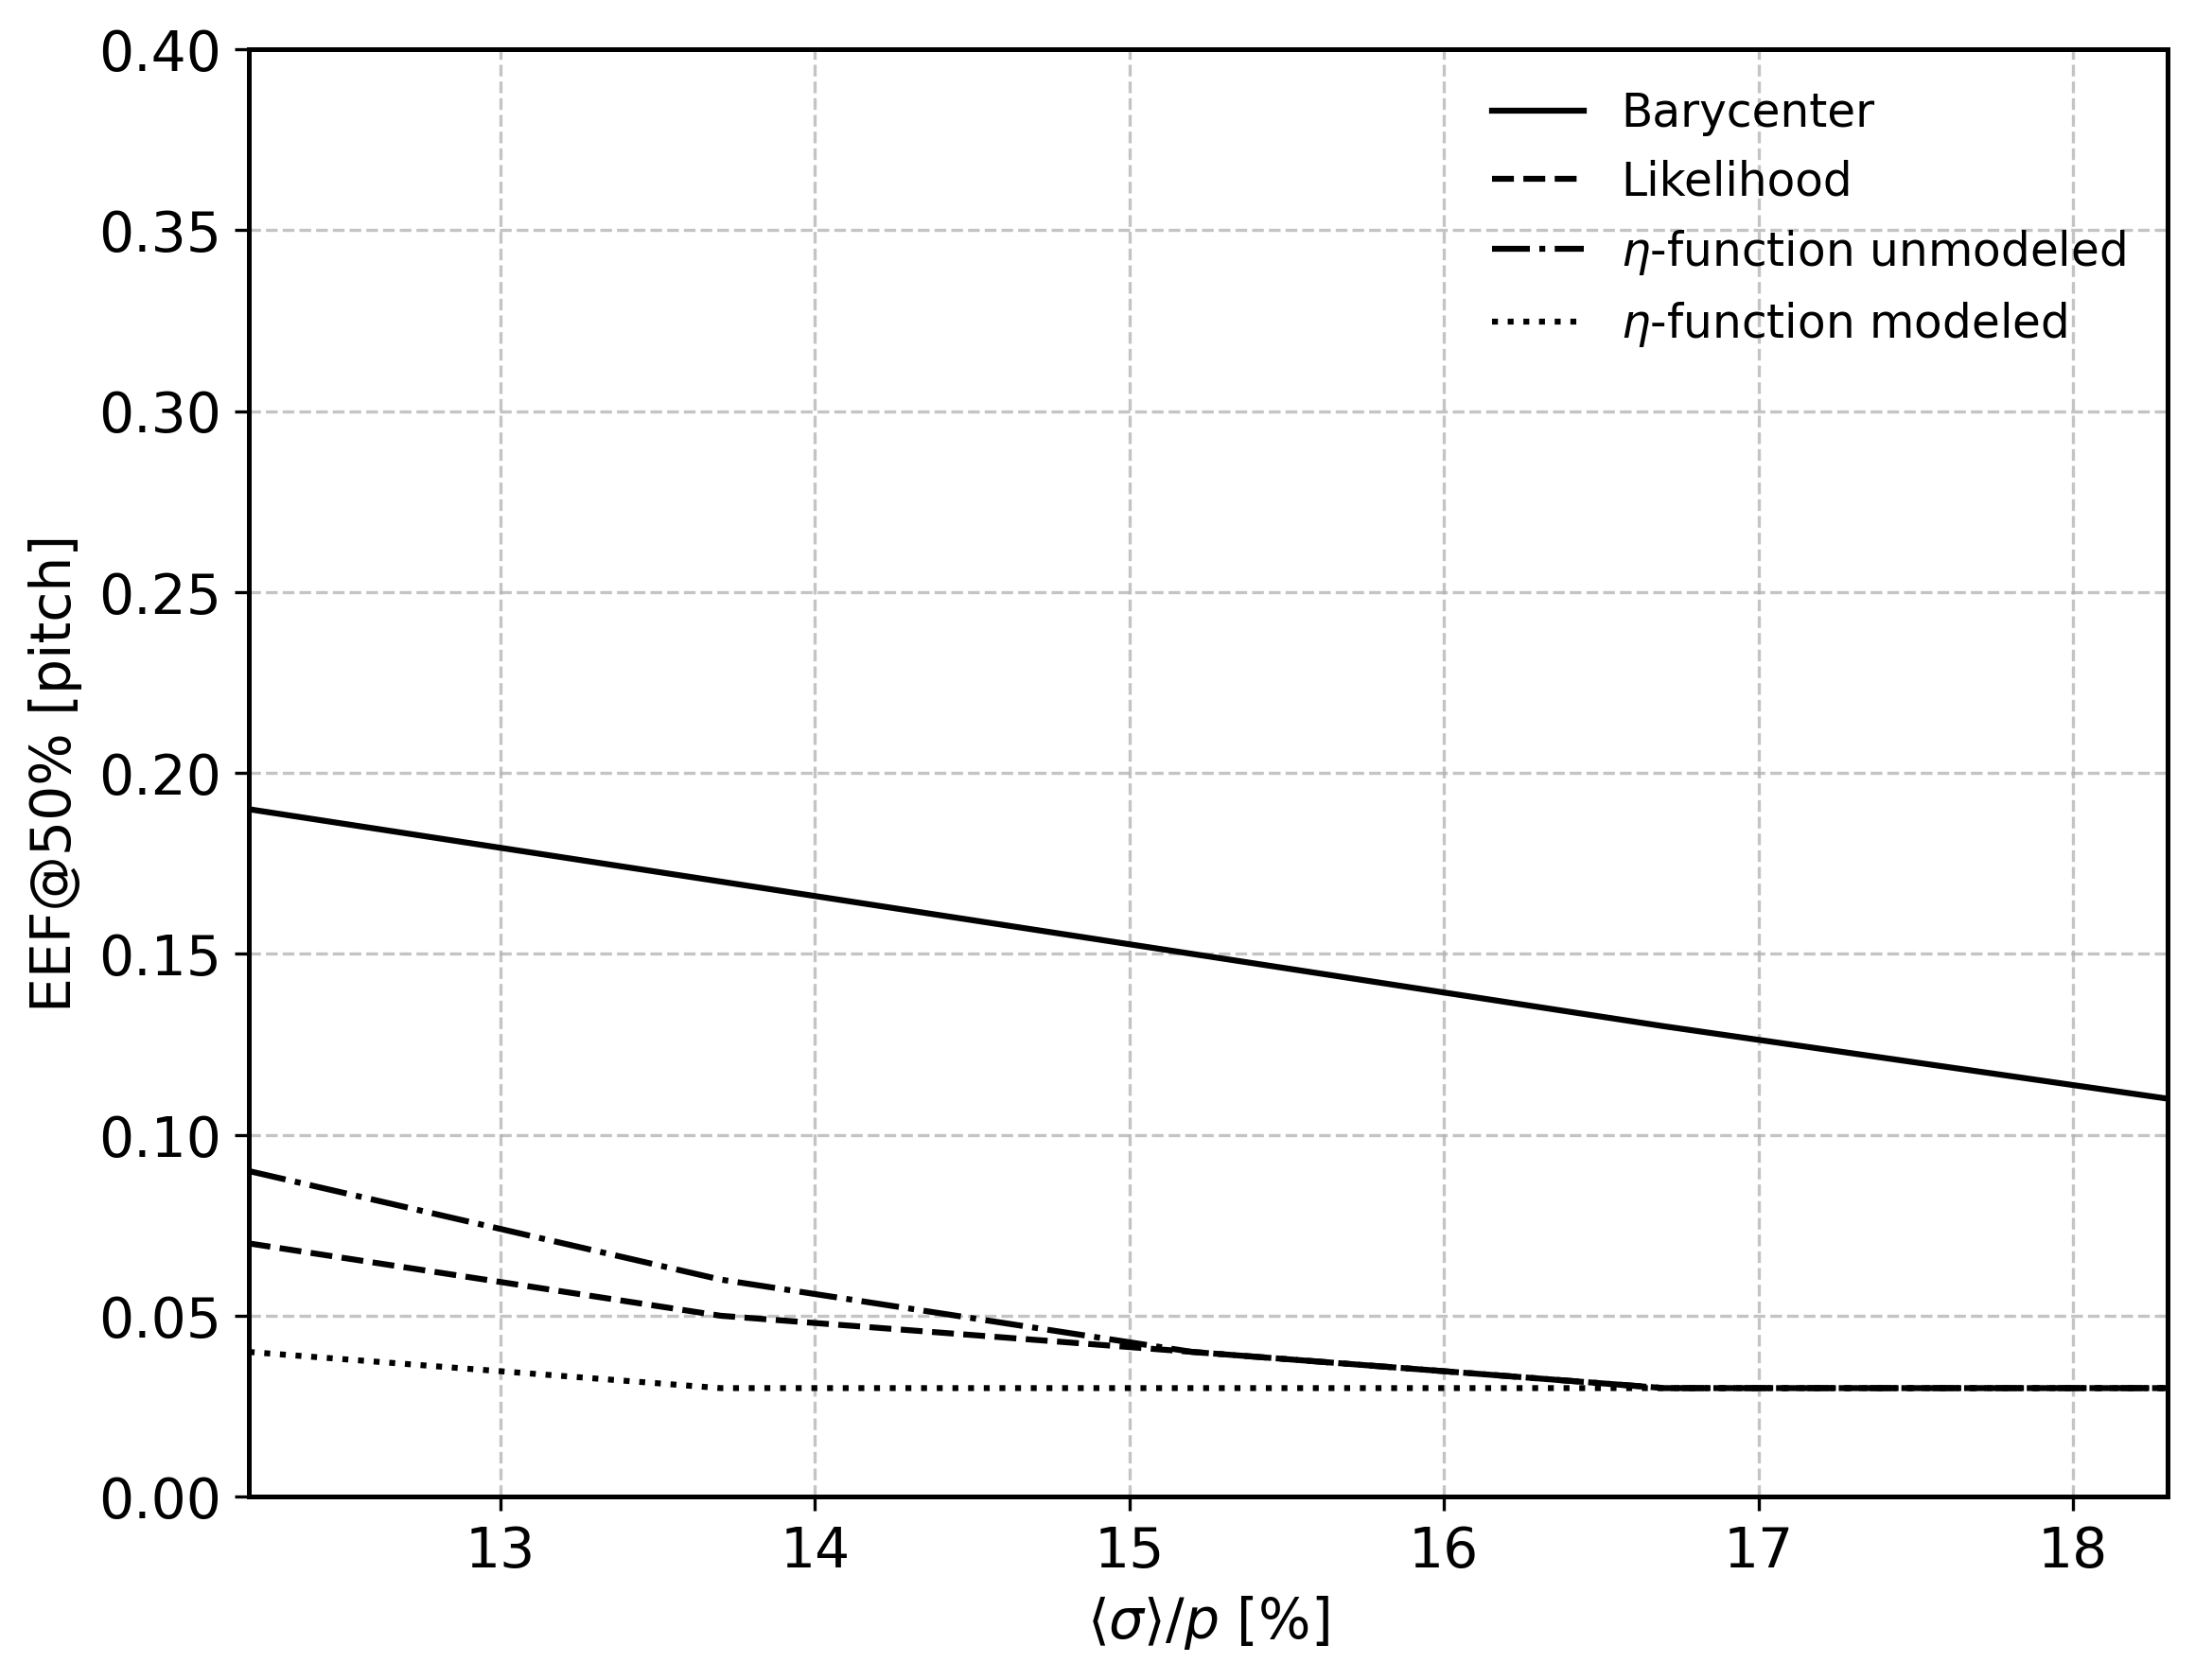
\includegraphics[width=0.49\linewidth]{figures/chapter4/position/eef50}
    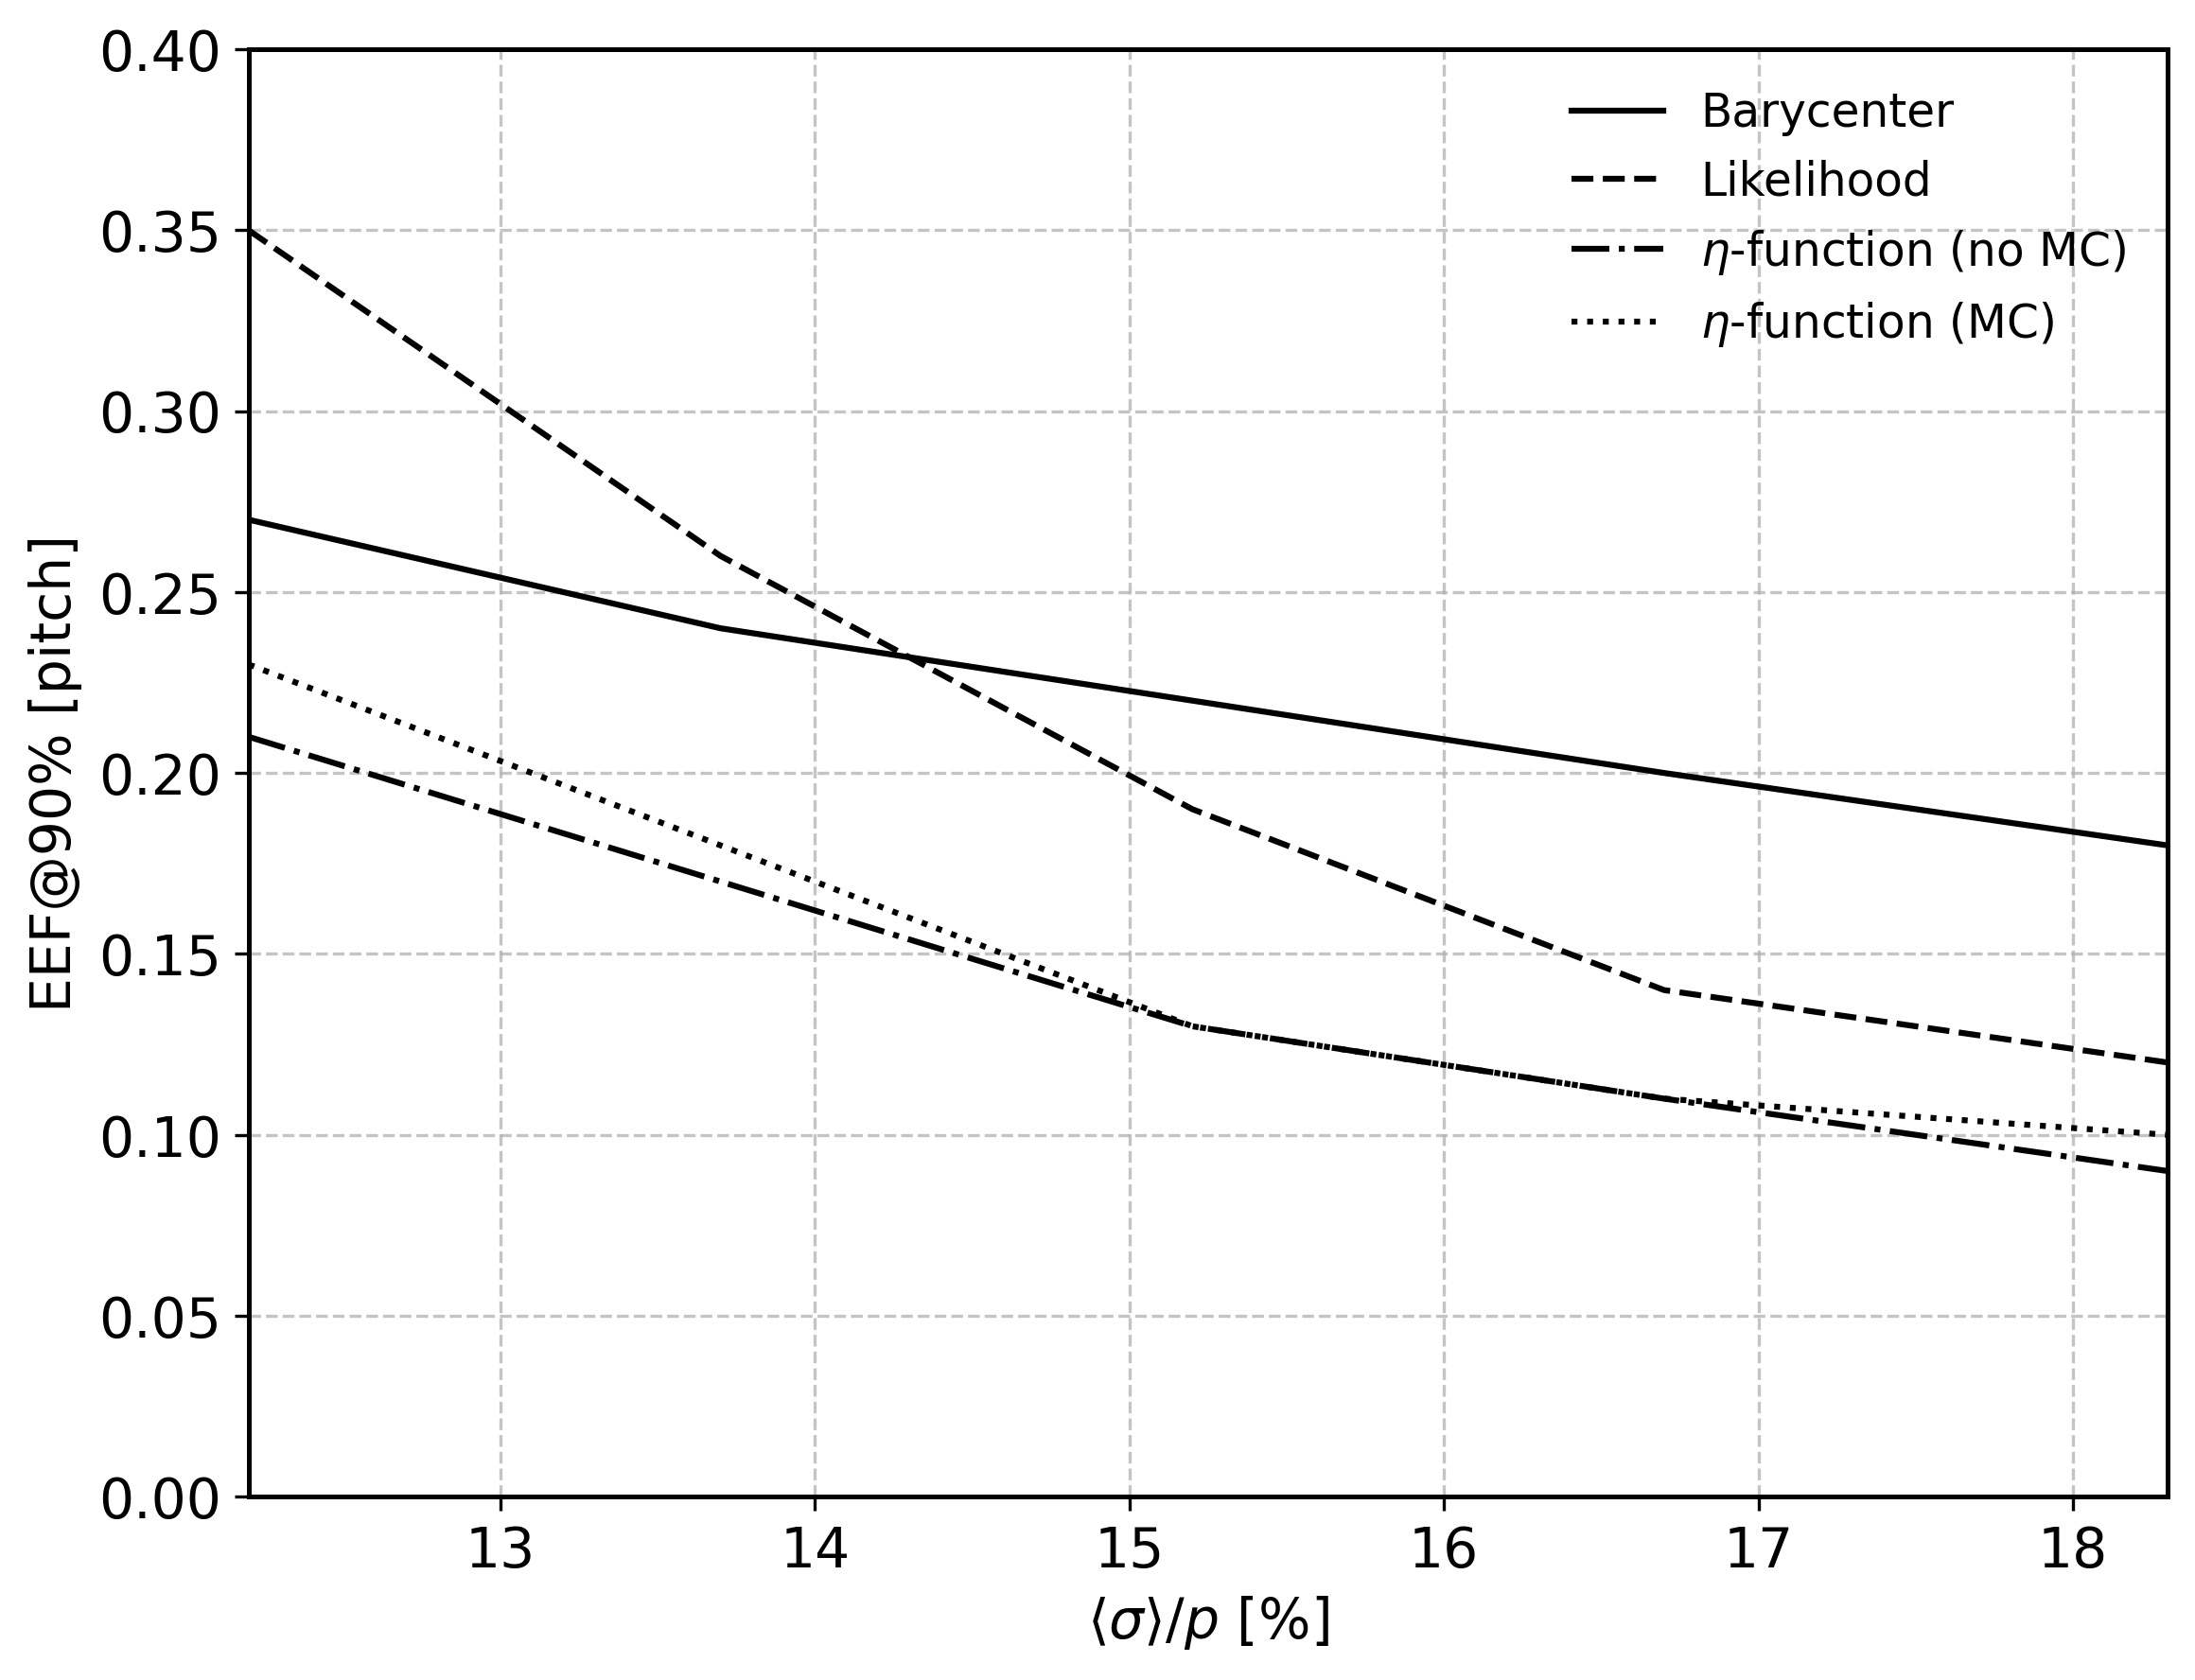
\includegraphics[width=0.49\linewidth]{figures/chapter4/position/eef90}
    \caption{EEF at 50\% (left panel) and 90\% (right panel) as a function of the ratio between the diffusion cloud sigma and the pixel pitch for all the position reconstruction algorithms. All the values are normalized to the pixel pitch.}
    \label{fig:eef}
\end{figure}

As visible in the left panel, the charge barycenter gives the worst core resolution for all diffusion regimes, with values of the EEF@50\% between 0.11 and 0.19 pitch. On the other hand, the MLE and the modeled $\eta$ algorithms achieve the best core containment, improving the EEF@50\% by up to a factor of four with respect to the charge barycenter. The unmodeled $\eta$ algorithm shows slightly worse results than the modeled one for small diffusion widths, but reaches identical values for broader diffusions.

Considering the tails of the distributions, shown in the right panel with the EEF@90\%, the situation is different. For small values of $\langle \sigma \rangle / p$, the MLE has very long tails and its EEF@90\% is even worse than the charge barycenter. This does not happen for the $\eta$ algorithms, which maintain better tail containment across all diffusion regimes. Between the two, the modeled $\eta$ algorithm achieves the best overall performance.

%\begin{figure}[htbp]
%    \centering
%    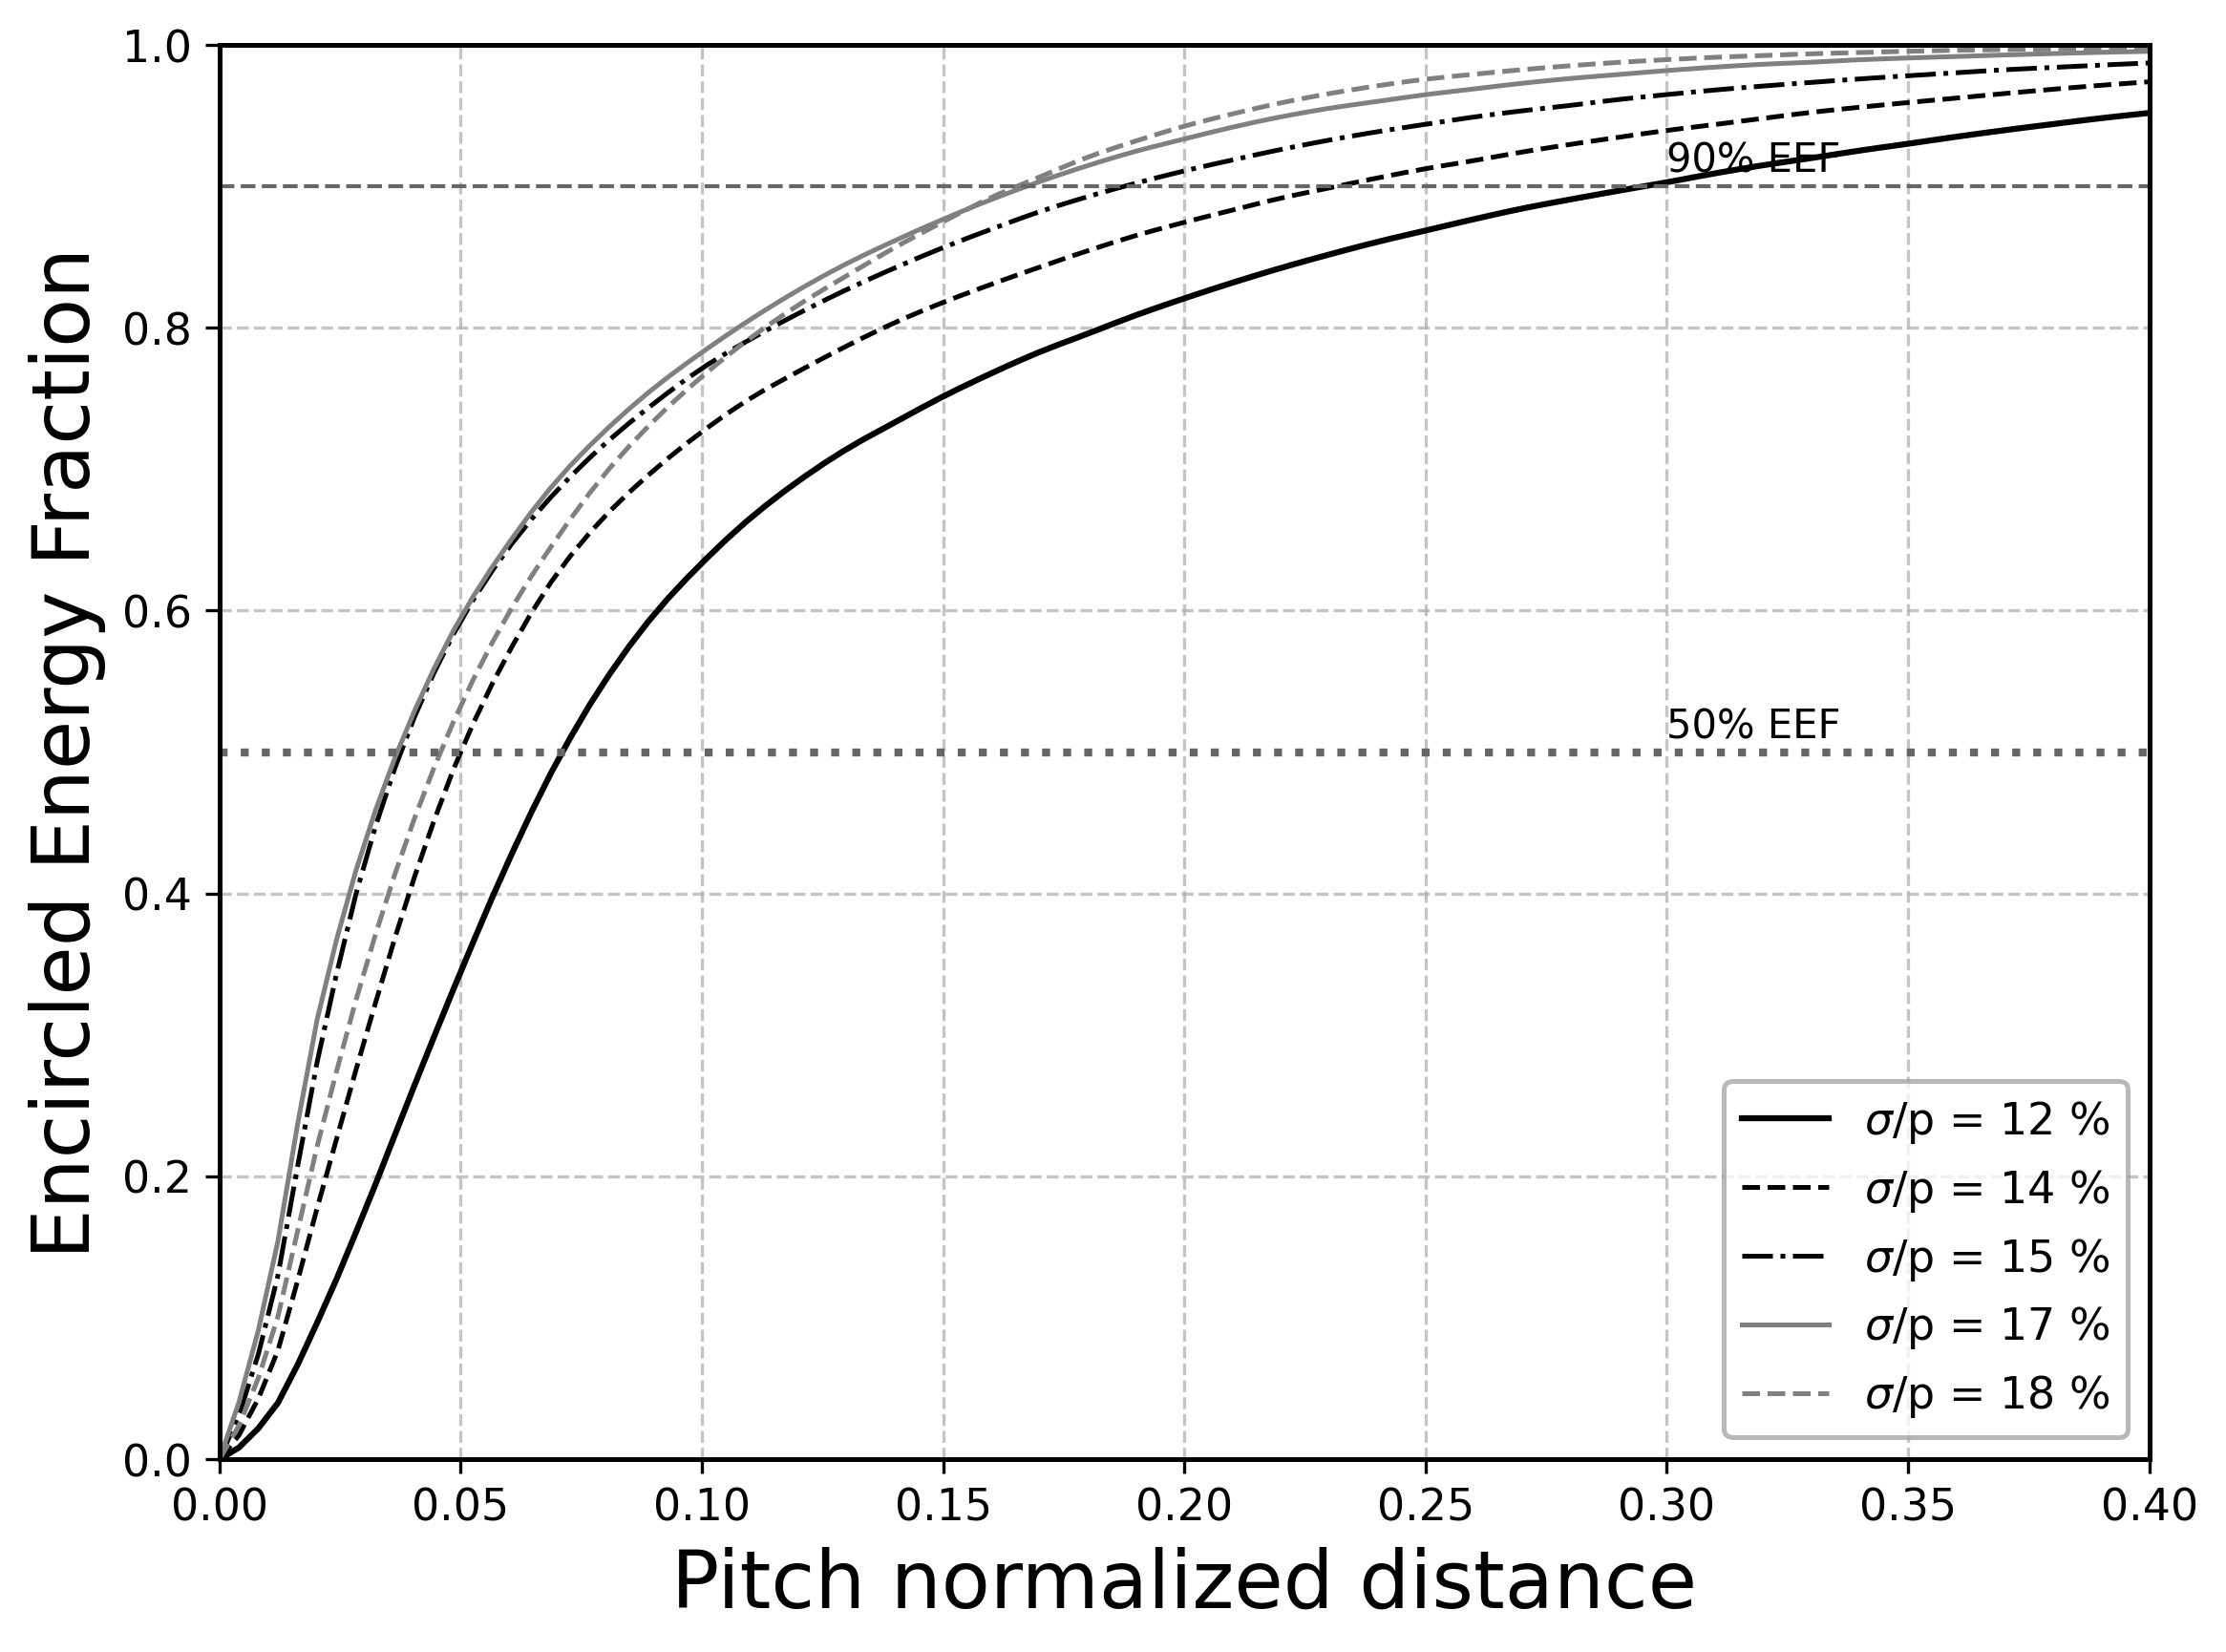
\includegraphics[width=0.49\linewidth]{figures/chapter4/position/mle_systematics}
%    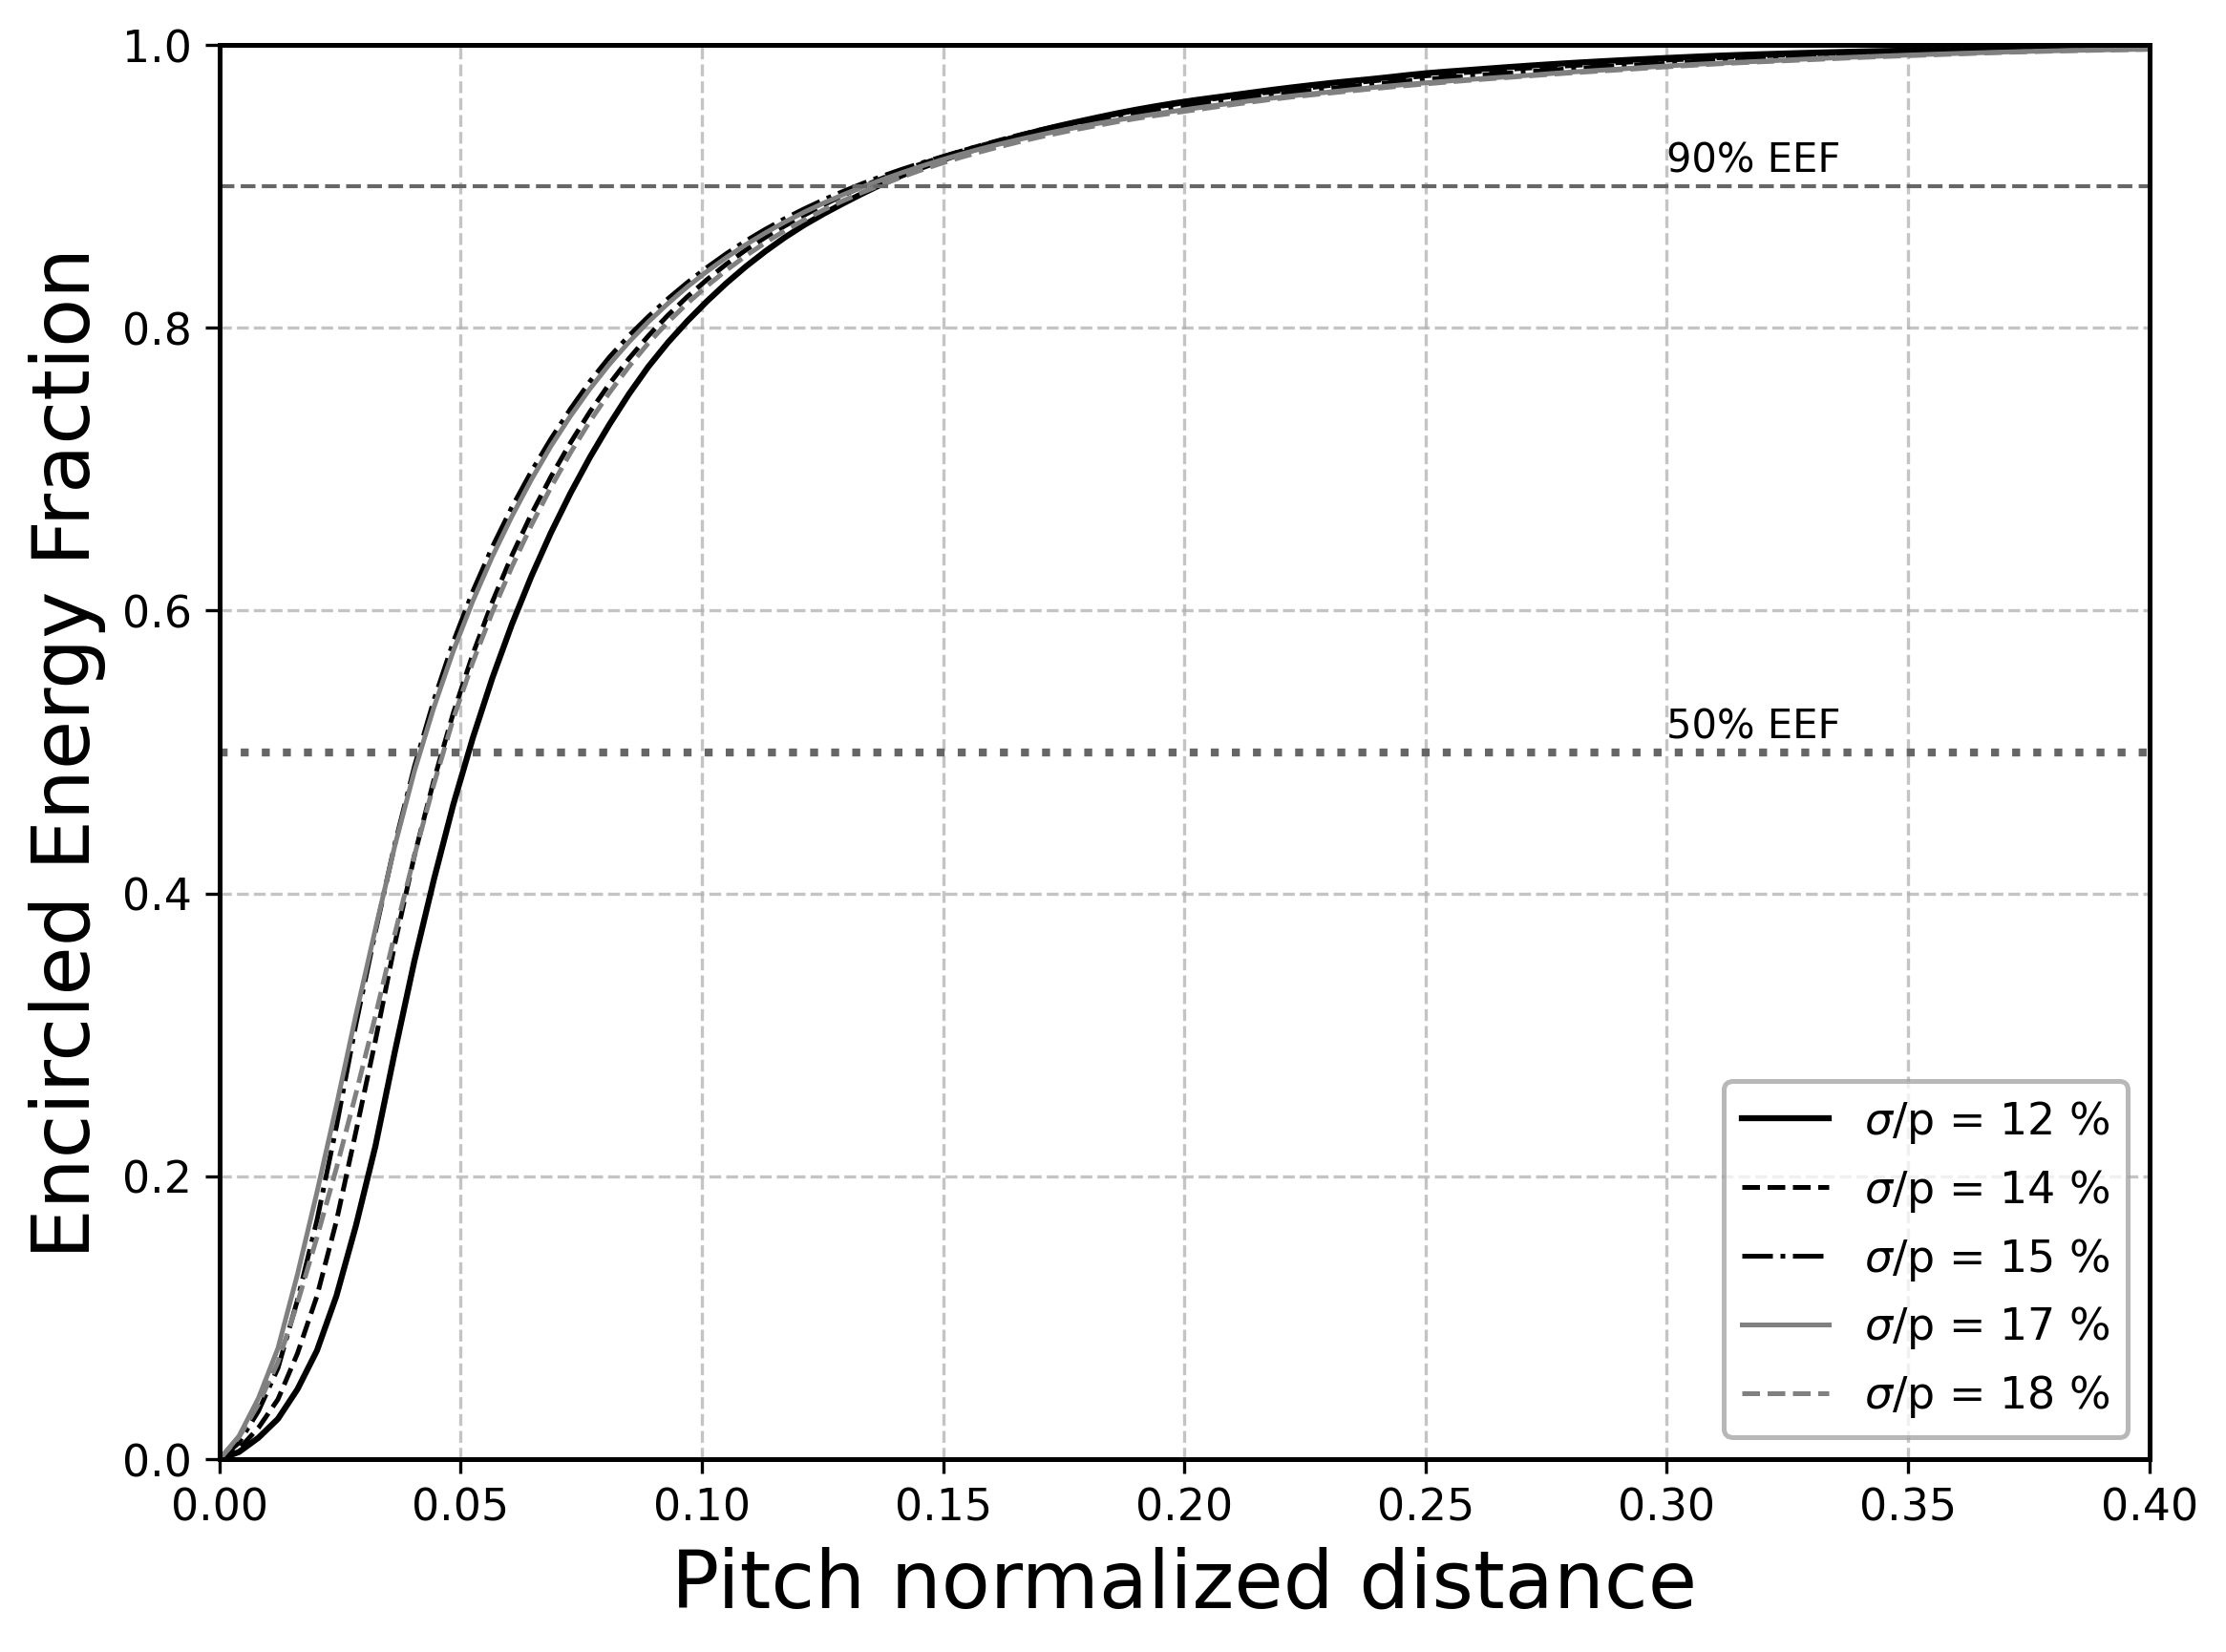
\includegraphics[width=0.49\linewidth]{figures/chapter4/position/eta_unmodeled_systematics}
%    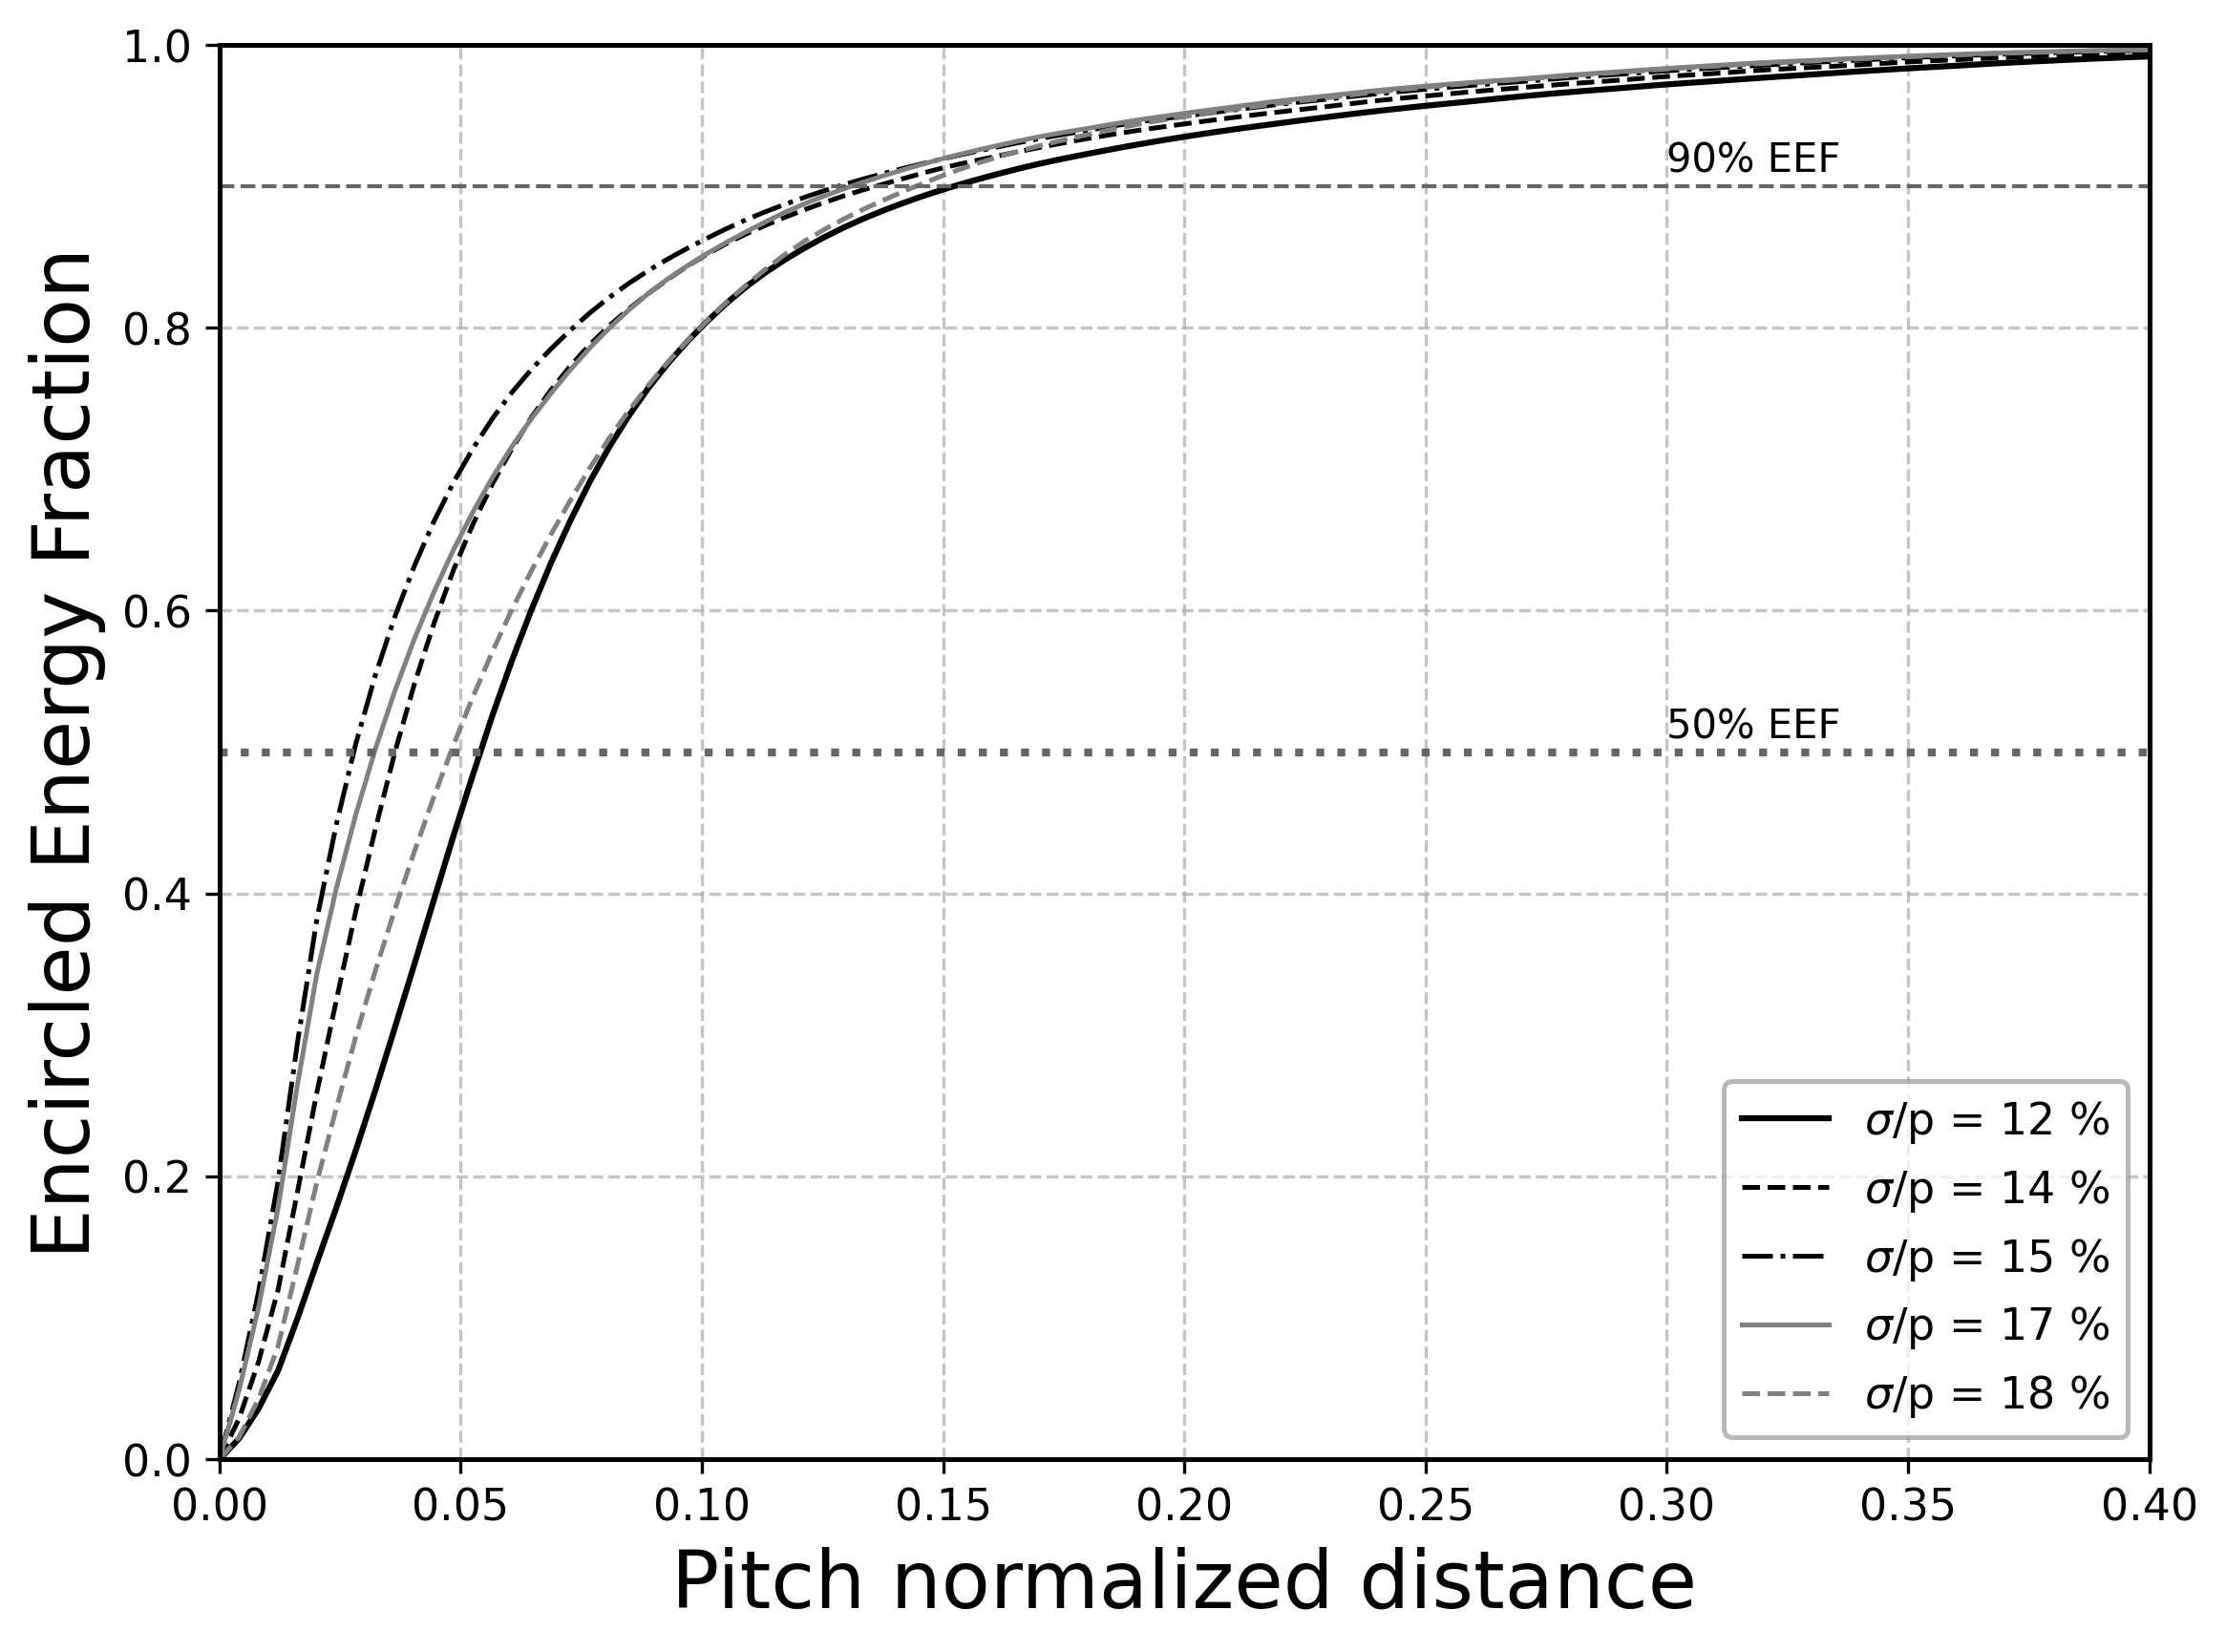
\includegraphics[width=0.49\linewidth]{figures/chapter4/position/eta_modeled_systematics}
%    \caption{}
%    \label{fig:eef_systematics}
%\end{figure}

Both the MLE and the modeled $\eta$ algorithms require an accurate calibration from Monte Carlo simulations, while the unmodeled $\eta$ relies on data from a uniform illumination. In a real scenario, systematic uncertainties in the Monte Carlo parameters can introduce an error in the assumed charge diffusion width.

To quantify how this mismatch affects the spatial resolution, the simulated dataset with a true $\langle \sigma \rangle / p = 15\%$ has been analyzed using "wrong" calibrations generated for different values of $\langle \sigma \rangle / p$. The relative variation of the EEF is reported in Tab. \ref{tab:variation_eef}.

The results show that the MLE and the modeled $\eta$ algorithms are very sensitive to calibration errors. If the diffusion width is not exact, the core resolution drastically worsens, with the EEF@50\% increasing up to almost 90\% for the MLE. On the other hand, the unmodeled $\eta$ algorithm is much more stable. Even with a large mismatch, its core resolution degrades by a maximum of 25\%, and its tails (EEF@90\%) are almost completely unaffected. This means that if Monte Carlo simulations are not perfectly tuned, the unmodeled $\eta$ algorithm is the most reliable choice.

\begin{table}[!t]
\centering
\begin{tabularx}{\textwidth}{X ccccc}

Reconstruction Algorithm & \multicolumn{5}{c}{$\langle \sigma \rangle / p$ [\%]} \\
\cmidrule(l){2-6}
 & 12 & 14 & 15 & 17 & 18 \\
\midrule
MLE & & & & & \\
\quad EEF@50\% & 189\% & 133\% & 100\% & 98\%  & 122\% \\
\quad EEF@90\% & 157\% & 124\% & 100\% & 89\%  & 88\%  \\
\midrule
Unmodeled $\eta$ & & & & & \\
\quad EEF@50\% & 125\% & 112\% & 100\% & 101\% & 112\% \\
\quad EEF@90\% & 103\% & 101\% & 100\% & 101\% & 103\% \\
\midrule
Modeled $\eta$ & & & & & \\
\quad EEF@50\% & 194\% & 131\% & 100\% & 115\% & 172\% \\
\quad EEF@90\% & 119\% & 106\% & 100\% & 102\% & 112\% \\
\bottomrule
\end{tabularx}
\caption{Relative variation of the EEF@50\% and EEF@90\% obtained by analyzing a dataset with true $\langle \sigma \rangle / p = 15\%$ using calibrations generated with different diffusion widths. Values are normalized to the optimal calibration at 15\%, which corresponds to 100\%.}
\label{tab:variation_eef}
\end{table}

\subsection{Modulation transfer function}
\label{subsec:mtf}

A method that is commonly applied in medical physics to characterize the imaging response of the detector is to produce the image of a linear object and study the detector response. This can be achieved using an absorber material plate, such as lead for X-rays, with a slit on it \cite{fujita1992}. The intensity profile of the image on the axis perpendicular to the slit as a function of the position is then calculated, and the result is called Line Spread Function (LSF) \cite{med_imaging}. More precisely, the LSF is the convolution of the PSF with the slit

\begin{equation}
\operatorname{LSF}(x) = \operatorname{PSF}(x, y) \ast \operatorname{Slit}(x, y).
\end{equation}

To correctly characterize the LSF, the slit profile should approach a Dirac $\delta$-function, or at least the slit width should be much smaller than the expected resolution.

Another requirement for a better characterization is that the slit should be inclined with respect to the detector principal axes and the reason for this varies depending on the detector type. In case of energy integrating detectors, like those commonly used in radiography, the reason is that a slit aligned to an axis would produce a narrow LSF profile only a few pixels wide, thus it would be under-sampled. Instead, using an inclined slit causes pixels in adjacent rows to be hit in different positions, allowing to sample the LSF with sub-pixel sampling, which is called presampled LSF.

For single-photon driven readout detectors like ASIX, for which each photon is independently reconstructed with sub-pixel resolution, the reason to use a tilted slit is to uniformly sample the pixel. This enables to estimate the average resolution of the detector for the entire pixel, not only for a specific region. An example of the geometry of the detector and the slits is shown if Fig. \ref{fig:hex_grid_slits}.

The typical angle of the slit should be small, between 2 and 8 degrees, and should be far from being aligned to the main axes of the detector.

\begin{figure}[htbp]
    \centering
    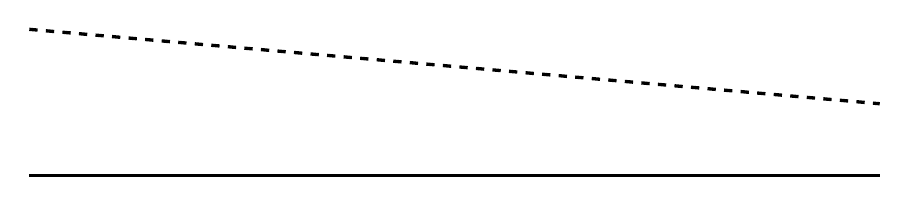
\begin{tikzpicture}[scale=1.2]
    
    \foreach \row in {-2,-1,0,1,2} {
        \foreach \col in {-4,-3,-2,-1,0,1,2,3,4} {
            \pgfmathsetmacro{\xpos}{\col + 0.5*mod(abs(\row),2)}
            \pgfmathsetmacro{\ypos}{\row * 0.866025}

            \hexpix[xshift=\xpos cm, yshift=\ypos cm]{\hexsize}
        }
    }

	\tikzset{slitLine/.style={very thick, opacity=0.7}}
	\draw[very thick, black] (-4.5, -0.7) -- (4.5, -0.7);;
	\draw[very thick, black, dashed] (-4.5, 0.84375) -- (4.5, 0.05625);

    \end{tikzpicture}
    \caption{Example of a grid with hexagonal pixels with two slits passing above. The solid line represents a slit parallel to the horizontal axis of the detector and always crosses the pixels in the same region. The dashed line represents an inclined slit with an angle of 5 degrees, and it crosses different regions each time.}
    \label{fig:hex_grid_slits}
\end{figure}

Producing a slit with a width small enough for high-resolution detectors is not always possible. An alternative method to characterize the spatial resolution consists of using the sharp edge of a slab of absorber material.

The profile image of the transition region around the edge is called Edge Spread Function (ESF). As for the slit method, the edge method requires the edge to be slightly tilted with respect to the main axes of the detector. Similarly to the LSF, the ESF can be computed as

\begin{equation}
\operatorname{ESF}(x) = \operatorname{PSF}(x, y) \ast \operatorname{Edge}(x, y).
\end{equation}

The ideal edge should be perfectly sharp to not introduce distortions, thus it can be represented with a step function. Using the convolution properties, it is possible to show that the derivative of the ESF corresponds to the LSF

\begin{equation}
\frac{d}{dx} \operatorname{ESF}(x) = \operatorname{PSF}(x, y) \ast \frac{d}{dx} \operatorname{Edge}(x, y) = \operatorname{PSF}(x, y) \ast \operatorname{Line}(x, y) = \operatorname{LSF}(x).
\label{eq:esf_lsf}
\end{equation}

This relation holds also when the edge is not ideal.

Once the LSF has been sampled, either directly with a slit or indirectly with an edge using Eq. \ref{eq:esf_lsf}, it is possible to characterize the profile to determine the spatial resolution, that can be defined as the FWHM of the LSF.

The LSF and ESF are defined in the spatial domain. There is another quantity that is commonly used to characterize the imaging properties of a detector which is defined in the frequency domain, the modulation transfer function (MTF). The MTF is defined as the Fourier transform of the LSF

\begin{equation}
\operatorname{MTF}(f) = \mathcal{F}(\operatorname{LSF}(x)).
\label{eq:mtf}
\end{equation}

By definition, the amplitude of MTF is normalized in order to have $\operatorname{MTF}(0) = 1$, which can be achieved either by normalizing the LSF area to 1 or by dividing the resulting MTF by $\operatorname{MTF}(0)$.

The MTF measures how the contrast is transfered as a function of the spatial frequency of the incoming signal. A high value of the MTF for higher frequencies means that the detector has high contrast, thus it can resolve small objects. For an ideal detector with infinite resolution the LSF is a Dirac-$\delta$ function and the resulting MTF is constant and equal to 1.

As for the LSF and the ESF, using a tilted slit or edge to increase the sampling frequency enables to compute the presampled MTF \cite{samei1998}. The usual metric used to determine the spatial resolution of a detector is related to the frequency $f_{10}$ for which $\operatorname{MTF}(f_{10}) = 0.1$.

If the LSF is described by a Gaussian curve $f_{10}$ can be related to its standard deviation. By considering that the Fourier transform of a Gaussian is still a Gaussian

\begin{equation}
\mathcal{F} \left( \frac{1}{\sqrt{2 \pi}\sigma} e^{-x^2/2\sigma^2 } \right) (f) = e^{-2 \pi^2 \sigma^2 f^2},
\label{eq:mtf_gauss}
\end{equation}
and imposing that $\operatorname{MTF}(f_{10}) = 0.1$ it can be found that

\begin{equation}
\sigma = \sqrt{\frac{\ln 10}{2 \pi^2}} \frac{1}{f_{10}} \simeq \frac{1}{2.93 \cdot f_{10}}.
\label{eq:mtf_sigma}
\end{equation}

In general the LSF is not Gaussian. A simple example is to consider an ideal detector without noise sources and composed by a grid of square pixels. If the detector is not capable of reconstructing sub-pixel positions the LSF can be represented by a constant function in the region occupied by the pixel and zero elsewhere. If the pixel has a width equal to $d$ and goes from $-d/2$ and $d/2$, the resulting MTF is \cite{med_imaging}

\begin{equation}
\operatorname{MTF}(f) = \frac{\sin (\pi d f)}{\pi df} = \operatorname{sinc}(df).
\label{eq:mtf_square}
\end{equation}

Eq. \ref{eq:mtf_square} describes the best spatial resolution achievable by a detector with square pixels and without sub-pixel reconstruction.

Considering hexagonal pixels instead of square ones, it is possible to determine the intrinsic resolution achievable by ASIX assuming no sub-pixel reconstruction is employed and all the charge is assigned to the central pixel of the cluster.

The two-dimensional $\operatorname{MTF}(f_x, f_y)$ of an hexagonal pixel has been calculated in \cite{barnard1991} and the projections along the axes orthogonal to the side (0 degrees) and towards the vertex (30 degrees) for an hexagon with pitch $p$ are equal to

\begin{equation}
\begin{split}
\operatorname{MTF}(f_x, 0) = \frac{2}{3} \left[ \operatorname{sinc}(p f_x) + \frac{1}{2} \operatorname{sinc}^2\left( \frac{p}{2} f_x \right) \right], \\
\operatorname{MTF}(0, f_y) = \operatorname{sinc} \left( 	\frac{p}{2 \sqrt{3}} f_y	\right) \operatorname{sinc} \left( 	\frac{\sqrt{3} p}{2} f_y	\right).
\end{split}
\end{equation}

\begin{figure}[!t]
    \centering
    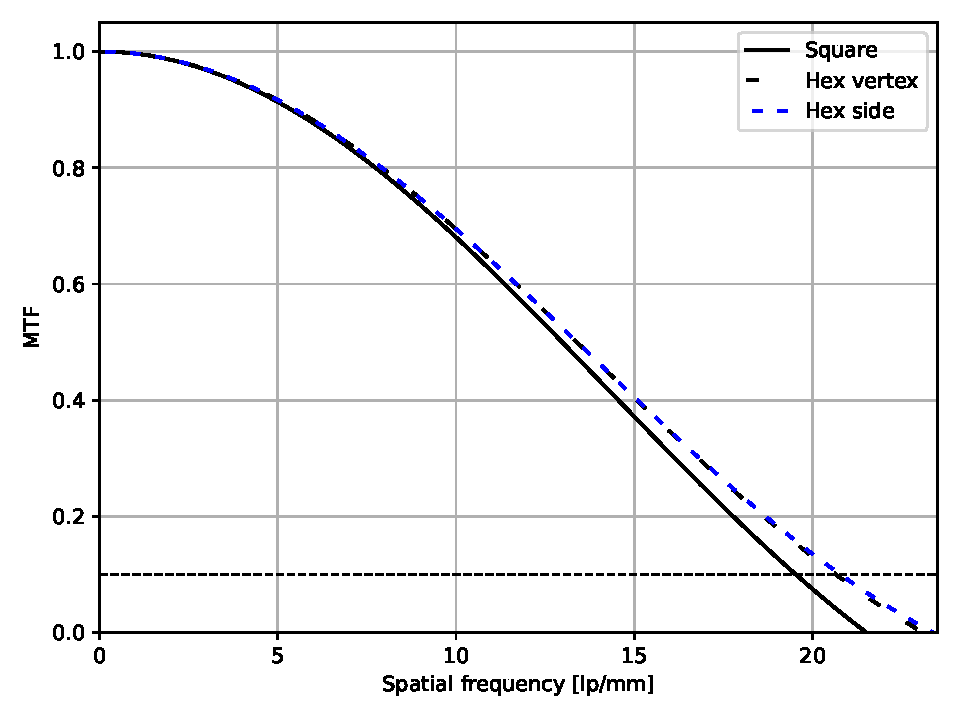
\includegraphics[width=0.6\linewidth]{figures/chapter4/position/mtf_hex_square}
    \caption{MTFs calculated for square and hexagonal pixels with same area. The hexagonal pixel pitch is $p = 50$ $\mu$m. The MTFs referred to the hexagonal pixel are calculated along the directions towards the vertex and orthogonal to the side.}
    \label{fig:mtf_pixels}
\end{figure}

Fig. \ref{fig:mtf_pixels} shows the comparison between the MTF of a square pixel and that of an hexagonal pixel with the same area. It is possible to see that the hexagonal geometry has a slightly better resolution than the square. This can be related to the highest degree of isotropy and symmetry of an hexagon with respect to a square.

Even if no noise sources have been considered for this estimate, it can be interpreted as a lower limit on the resolution of ASIX, as sub-pixel reconstruction algorithms using charge-sharing and diffusion models enable to improve the detector performance.

An alternative and faster way to estimate the spatial resolution of a detector consists of using a line pair phantom, which is a plate with multiple sets of slits with different widths and spatial frequencies, which are expressed as line pair or cycles per millimeter (lp/mm or cycles/mm). The phantom is made of an high-$Z$ material, usually lead. The resolution can be inferred from an image of the phantom by looking at which set of slits is the smallest that can be resolved. The only requirement to use this method is to have a set of slits with a frequency smaller or comparable to the spatial resolution of the detector, but this may not be possible for high resolution detectors.


\begin{figure}[!t]
    \centering
    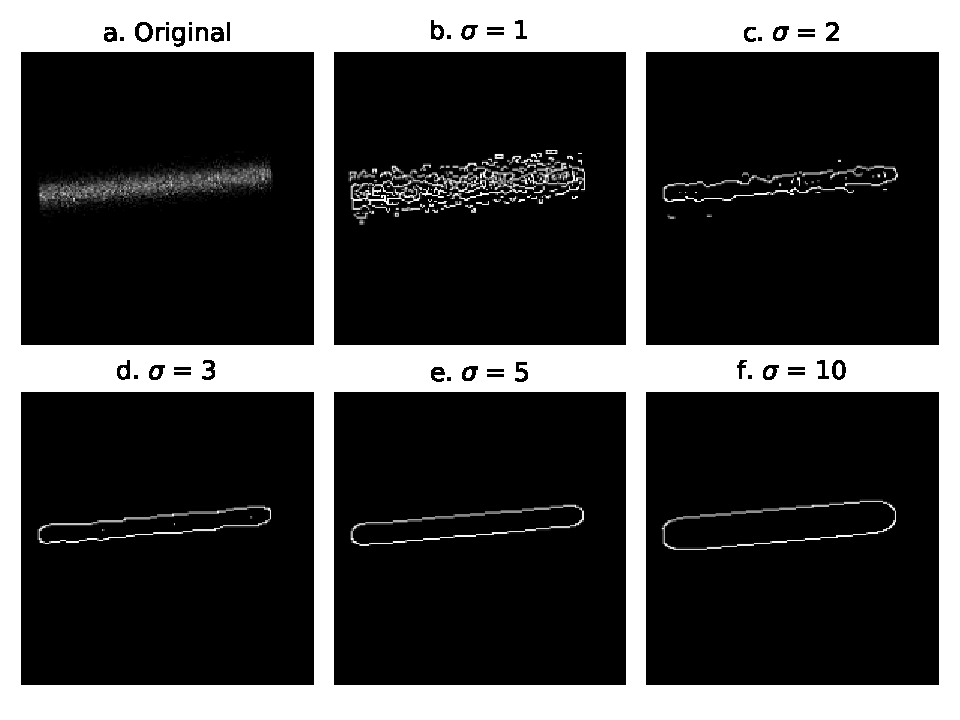
\includegraphics[width=0.8\linewidth]{figures/chapter4/position/mtf_canny}
    \caption{Example usage of the Canny edge detection algorithm on a simulated slit image. The simulated image (a) is binned with a $200 \times 200$ grid, while the slit has a Gaussian profile with a standard deviation of 5 pixels, a length of 160 pixels and a tilt angle of 5 degrees. Images from (b) to (f) show how the detected edges vary by changing the Gaussian filter width. A filter to small is very sensitive to low statistics and detects false edges. Increasing the filter width, this effect becomes less and less visible. If the filter is too wide with respect to the slit width, no edge is detected (case not shown).}
    \label{fig:mtf_canny}
\end{figure}

When using a tilted slit or edge to calculate the MTF, it is necessary to calculate the tilt angle to correctly project the LSF or ESF profile. The procedure to realign the image is described in the case of a slit, but it is the same for an edge.

The angle is determined by the inclination of the slit with respect to the detector $x$-axis. The first step consists of detecting the slit edges in the image. This can be performed using the Canny edge detection algorithm \cite{canny1986}. This algorithm allows to detect the edges in an image and returns a binary image of the same size where a value of 1 means that a pixel is an edge and 0 if it is not.

Before using this algorithm it is necessary to create an image by binning the reconstructed positions. The bin size can not be too large, otherwise the shape and orientation of the slit would be distorted. Another parameter to choose is the width of the Gaussian filter applied by the algorithm to smooth the image. This parameter can not be to small with respect to the slit width, otherwise quantization noise would lead to the detection of false edges. The ideal value should be of the order of the slit width. An example of how the filter width affects edge detection is shown in Fig. \ref{fig:mtf_canny}.

The second step of the process consists of calculating the angle from the detected edges, which are sets of straight lines. This can be performed with the use of the Hough transform \cite{hough1959, duda1972}, which is a technique used to detect parameterizable curves, such as lines.

A line in the plane is represented by a set of two parameters $(\rho, \theta)$, which define the Hough space, where $\rho$ is the distance of the line from the origin of the axes and $\theta$ is the angle between the $x$-axis and the distance vector. Within this representation, each point $(x, y)$ on a straight line is described by

\begin{equation}
\rho = x \cos \theta + y \sin \theta.
\label{eq:hough}
\end{equation}

\begin{figure}[!t]
    \centering
    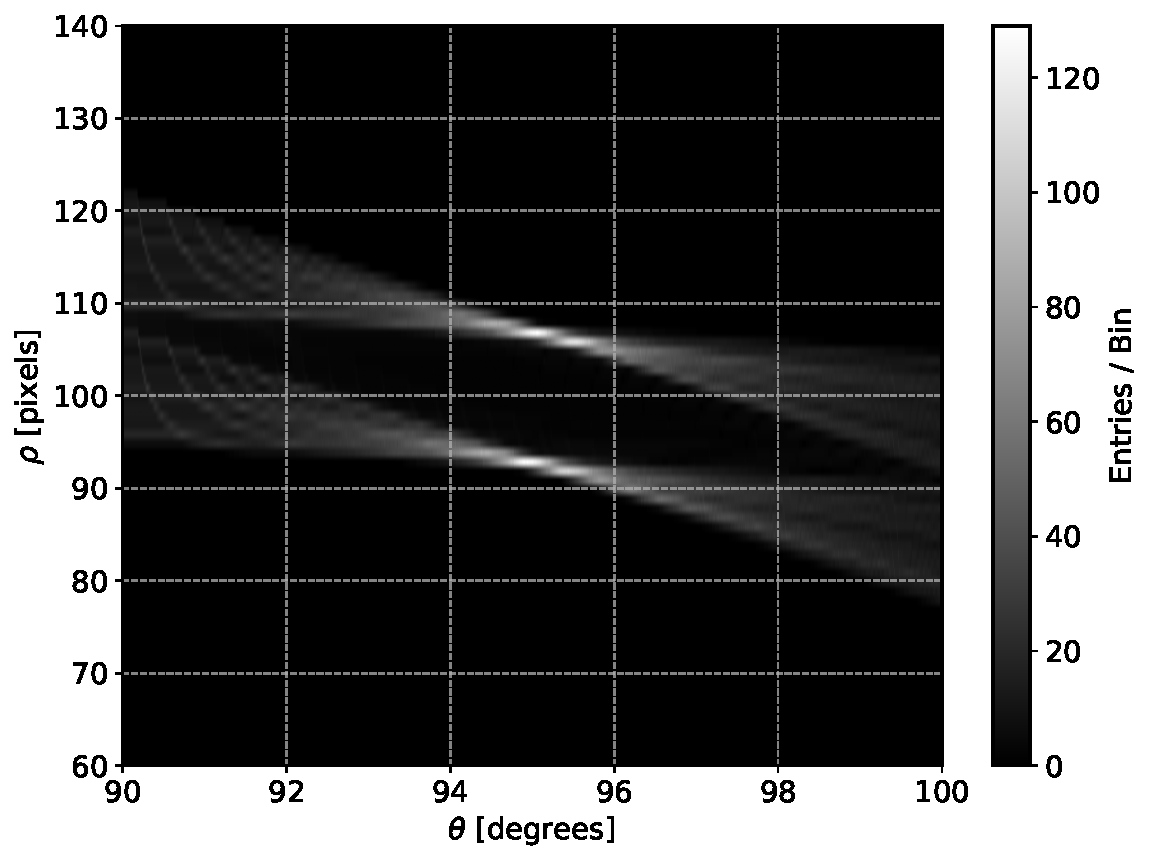
\includegraphics[width=0.7\linewidth]{figures/chapter4/position/mtf_hough}
    \caption{Accumulator space resulting from the Hough transform of the slit edge image from Fig. \ref{fig:mtf_canny}(e). The two nearly identical peaks that are visible correspond to the two long edges of the slit.}
    \label{fig:mtf_hough}
\end{figure}

For each point of the edges, the algorithm scans a given range of $\theta$ values and for each one evaluates Eq. \ref{eq:hough}. The results are accumulated in a two-dimensional histogram, named accumulator space, where for each point and angle value an entry is added at the correspondent bin $(\rho, \theta)$. A straight line is detected when a peak is identified in the latter space, and the tilt angle can be calculated as $\theta_{peak} - \pi/2$. An example of the result of the Hough transform of the edges of a  slit is shown in Fig. \ref{fig:mtf_hough}. During the analysis, if multiple lines are present and multiple peaks are produced by the Hough transform, only the highest one is considered to calculate the tilt angle.

To calculate the presampled LSF, the slit image has to be rotated by the angle found with the Hough transform. Once it has been aligned, the presampled LSF is calculated projecting all the points on the short side of the slit and calculating the histogram of the reconstructed positions. The bin size of this histogram must be smaller than the expected resolution of the detector, in order to not incur in aliasing effects, as stated by the Nyquist theorem, but large enough to not be sensitive to noise.

A possible way to limit distortions from noise is to apply a smoothing algorithm on the LSF, but remembering that in frequency domain a smoothing acts as a low-pass filter, with the possible consequence of underestimating the actual detector resolution.

The presampled MTF is then calculated from the LSF using a discrete fast Fourier transform algorithm. The LSF and MTF calculated from the previous examples are shown in Fig. \ref{fig:slit_lsf_mtf}.

In conclusion, the MTF currently represents the only available way to characterize the spatial resolution of the ASIX prototypes, and this analysis can be performed both on real and simulated data, in order to verify the consistency between the difference of the various implemented reconstruction algorithm and also the consistency between data and simulations.

\begin{figure}[h]
    \centering
    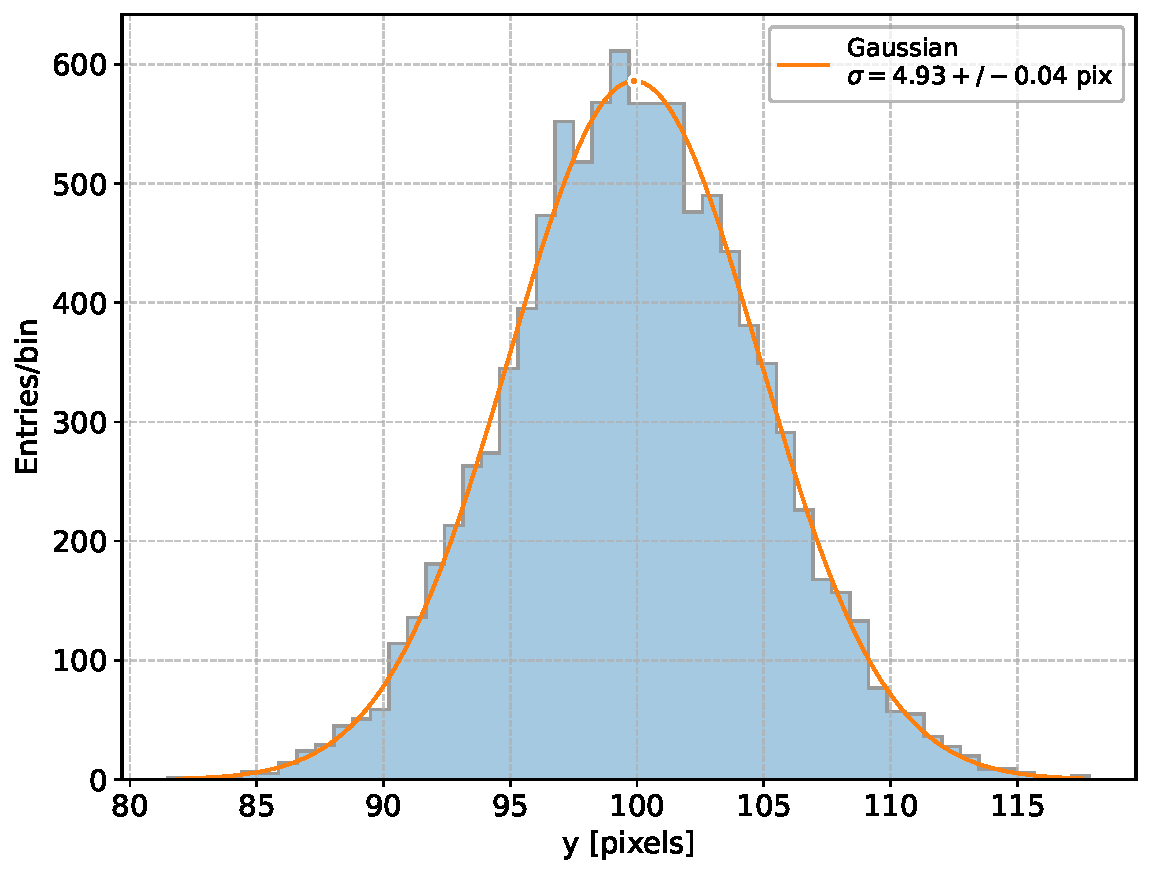
\includegraphics[width=0.49\linewidth]{figures/chapter4/position/mtf_lsf}
	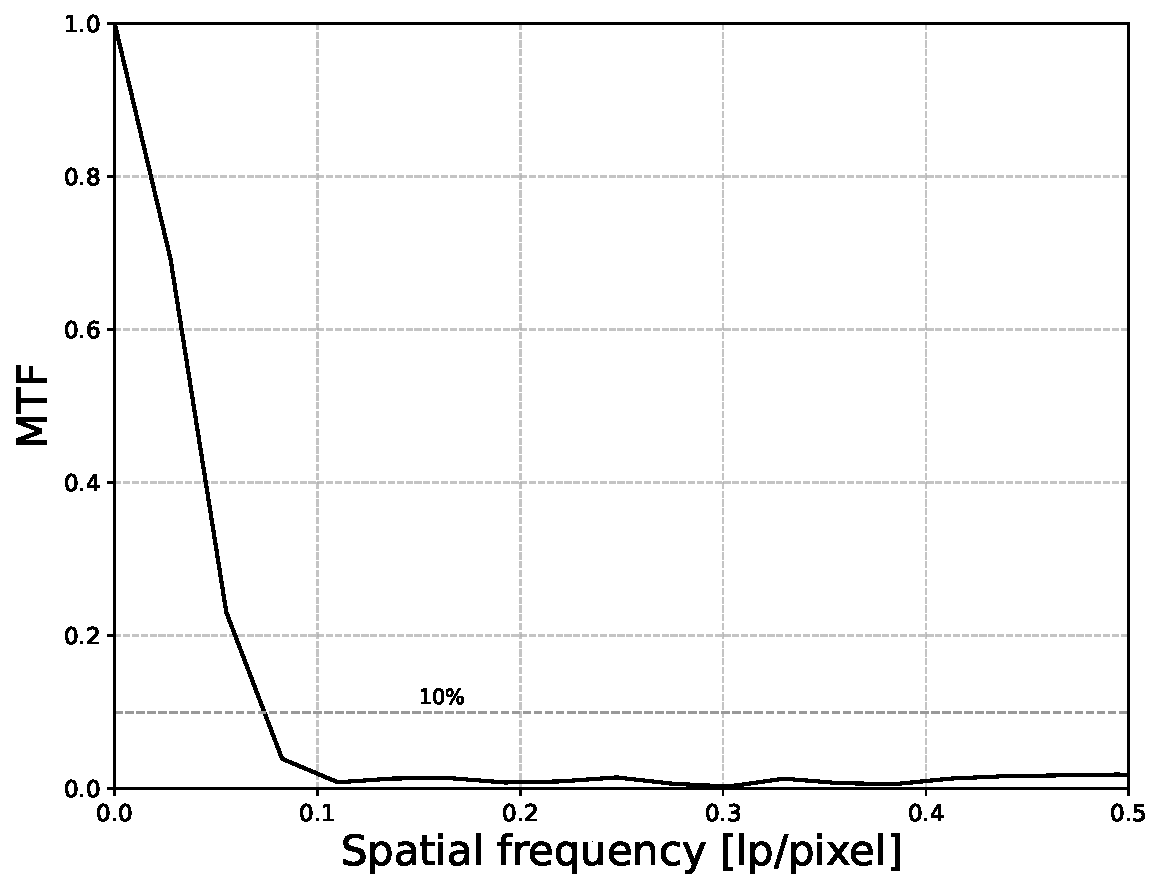
\includegraphics[width=0.49\linewidth]{figures/chapter4/position/mtf}
    \caption{Line spread function (left panel) and modulation transfer function (right panel) calculated for the slit using the edges from Fig. \ref{fig:mtf_canny}(e) and the tilt angle from \ref{fig:mtf_hough}. The slit was simulated with a Gaussian profile with $\sigma = 5$ pix. The standard deviation estimated from an LSF fit is $\sigma_{\textrm{fit}} = 4.93 \pm 0.04$ pix, while from the MTF is $\sigma_{\operatorname{MTF}} = 4.7$ pix using Eq. \ref{eq:mtf_sigma}.}
    \label{fig:slit_lsf_mtf}
\end{figure}


\section{Energy reconstruction}
Using the calibration products it is possible to estimate the photon energy for each event and calculating the spectrum of a source. If the absolute gain has been calibrated, the spectrum can be expressed in terms of eV instead of ADC counts if only the normalized gain has been calibrated. However, the difference is only a scale factor, thus it is not relevant.

As for position reconstruction, there are different algorithms that can be employed in the energy reconstruction. Specifically, two algorithms have been developed and will be explained in this section.

The performances of these algorithms will be shown in Chap. \ref{sec:results}, where laboratory data will be analyzed and the results are compared to simulations. The metric to determine the goodness of these algorithms is the FWHM of a given spectral line.

\subsection{Suppression algorithm}
The first energy reconstruction method is based on the suppression algorithm described in Chap. \ref{sec:analysis}. This algorithm consists of suppressing some of the pixels in an event by using a charge and a geometrical constraint, in order to minimize the probability of including pixels with charge not produced by the photon.

The charge constraint consists of selecting a threshold value, expressed in terms of noise $\sigma$ for each pixel. If a pixel has an amount of charge smaller than the threshold it is suppressed, thus its charge is put to zero. The geometrical constraint follows from the charge diffusion model and it consists of requiring that all the pixels that are above the threshold are adjacent. Furthermore, given the small charge diffusion width, if more than three pixels are above threshold only the three adjacent pixels with the most charge are kept.

This is the same algorithm that is employed to determine an event cluster size and that is applied before position reconstruction when using charge barycentering and $\eta$ algorithms.

After suppressing the pixels, the photon energy is calculated by summing the charge collected by all the unsuppressed pixels.

This method has a free parameter that can be varied, which is the value of the zero-suppression threshold. The final energy resolution depends on this parameter, and it is important to find the best value. This dependence will be shown on laboratory data in the next section.

\subsection{Likelihood estimator}
The second method to estimate the photon energy is to use the likelihood estimator introduced in Chap. \ref{subsec:mle} for the position reconstruction. The likelihood that describes the charge diffusion depends both on the photon incident position and energy, as shown in  Eq. \ref{eq:nll_multivariate}.

This algorithm has been already explained in detail in the previous section, and contrary to the suppression method it does not require an arbitrary threshold. Indeed, the likelihood model intrinsically weights the pixel charges through a simultaneous minimization of both the incident position and the photon energy.

\section{Results}
\label{sec:results}
The detector's imaging and energy resolutions are directly determined by the performance of the position and energy reconstruction methods. To accurately assess these properties, specific datasets were employed for each task.

These datasets were collected in the laboratory using ASIX prototypes. As previously mentioned, the current prototypes are equipped with the XPOL-III ASIC, which differs from the final design in several aspects. The most significant difference is the electronic noise, which is currently four to five times higher than the design goal.

\begin{figure}[!b]
    \centering
    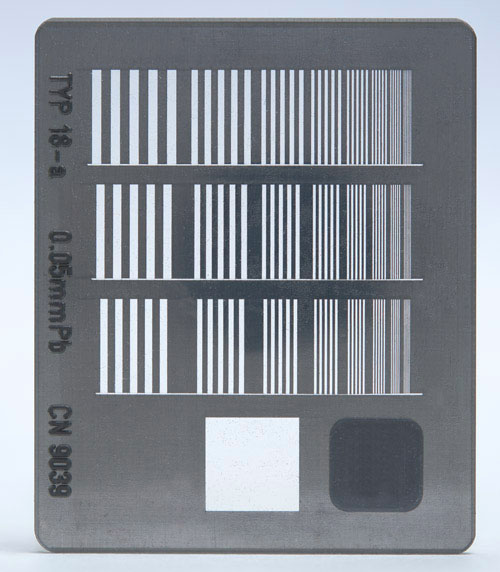
\includegraphics[width=0.4\linewidth]{figures/chapter4/results/huttner}
	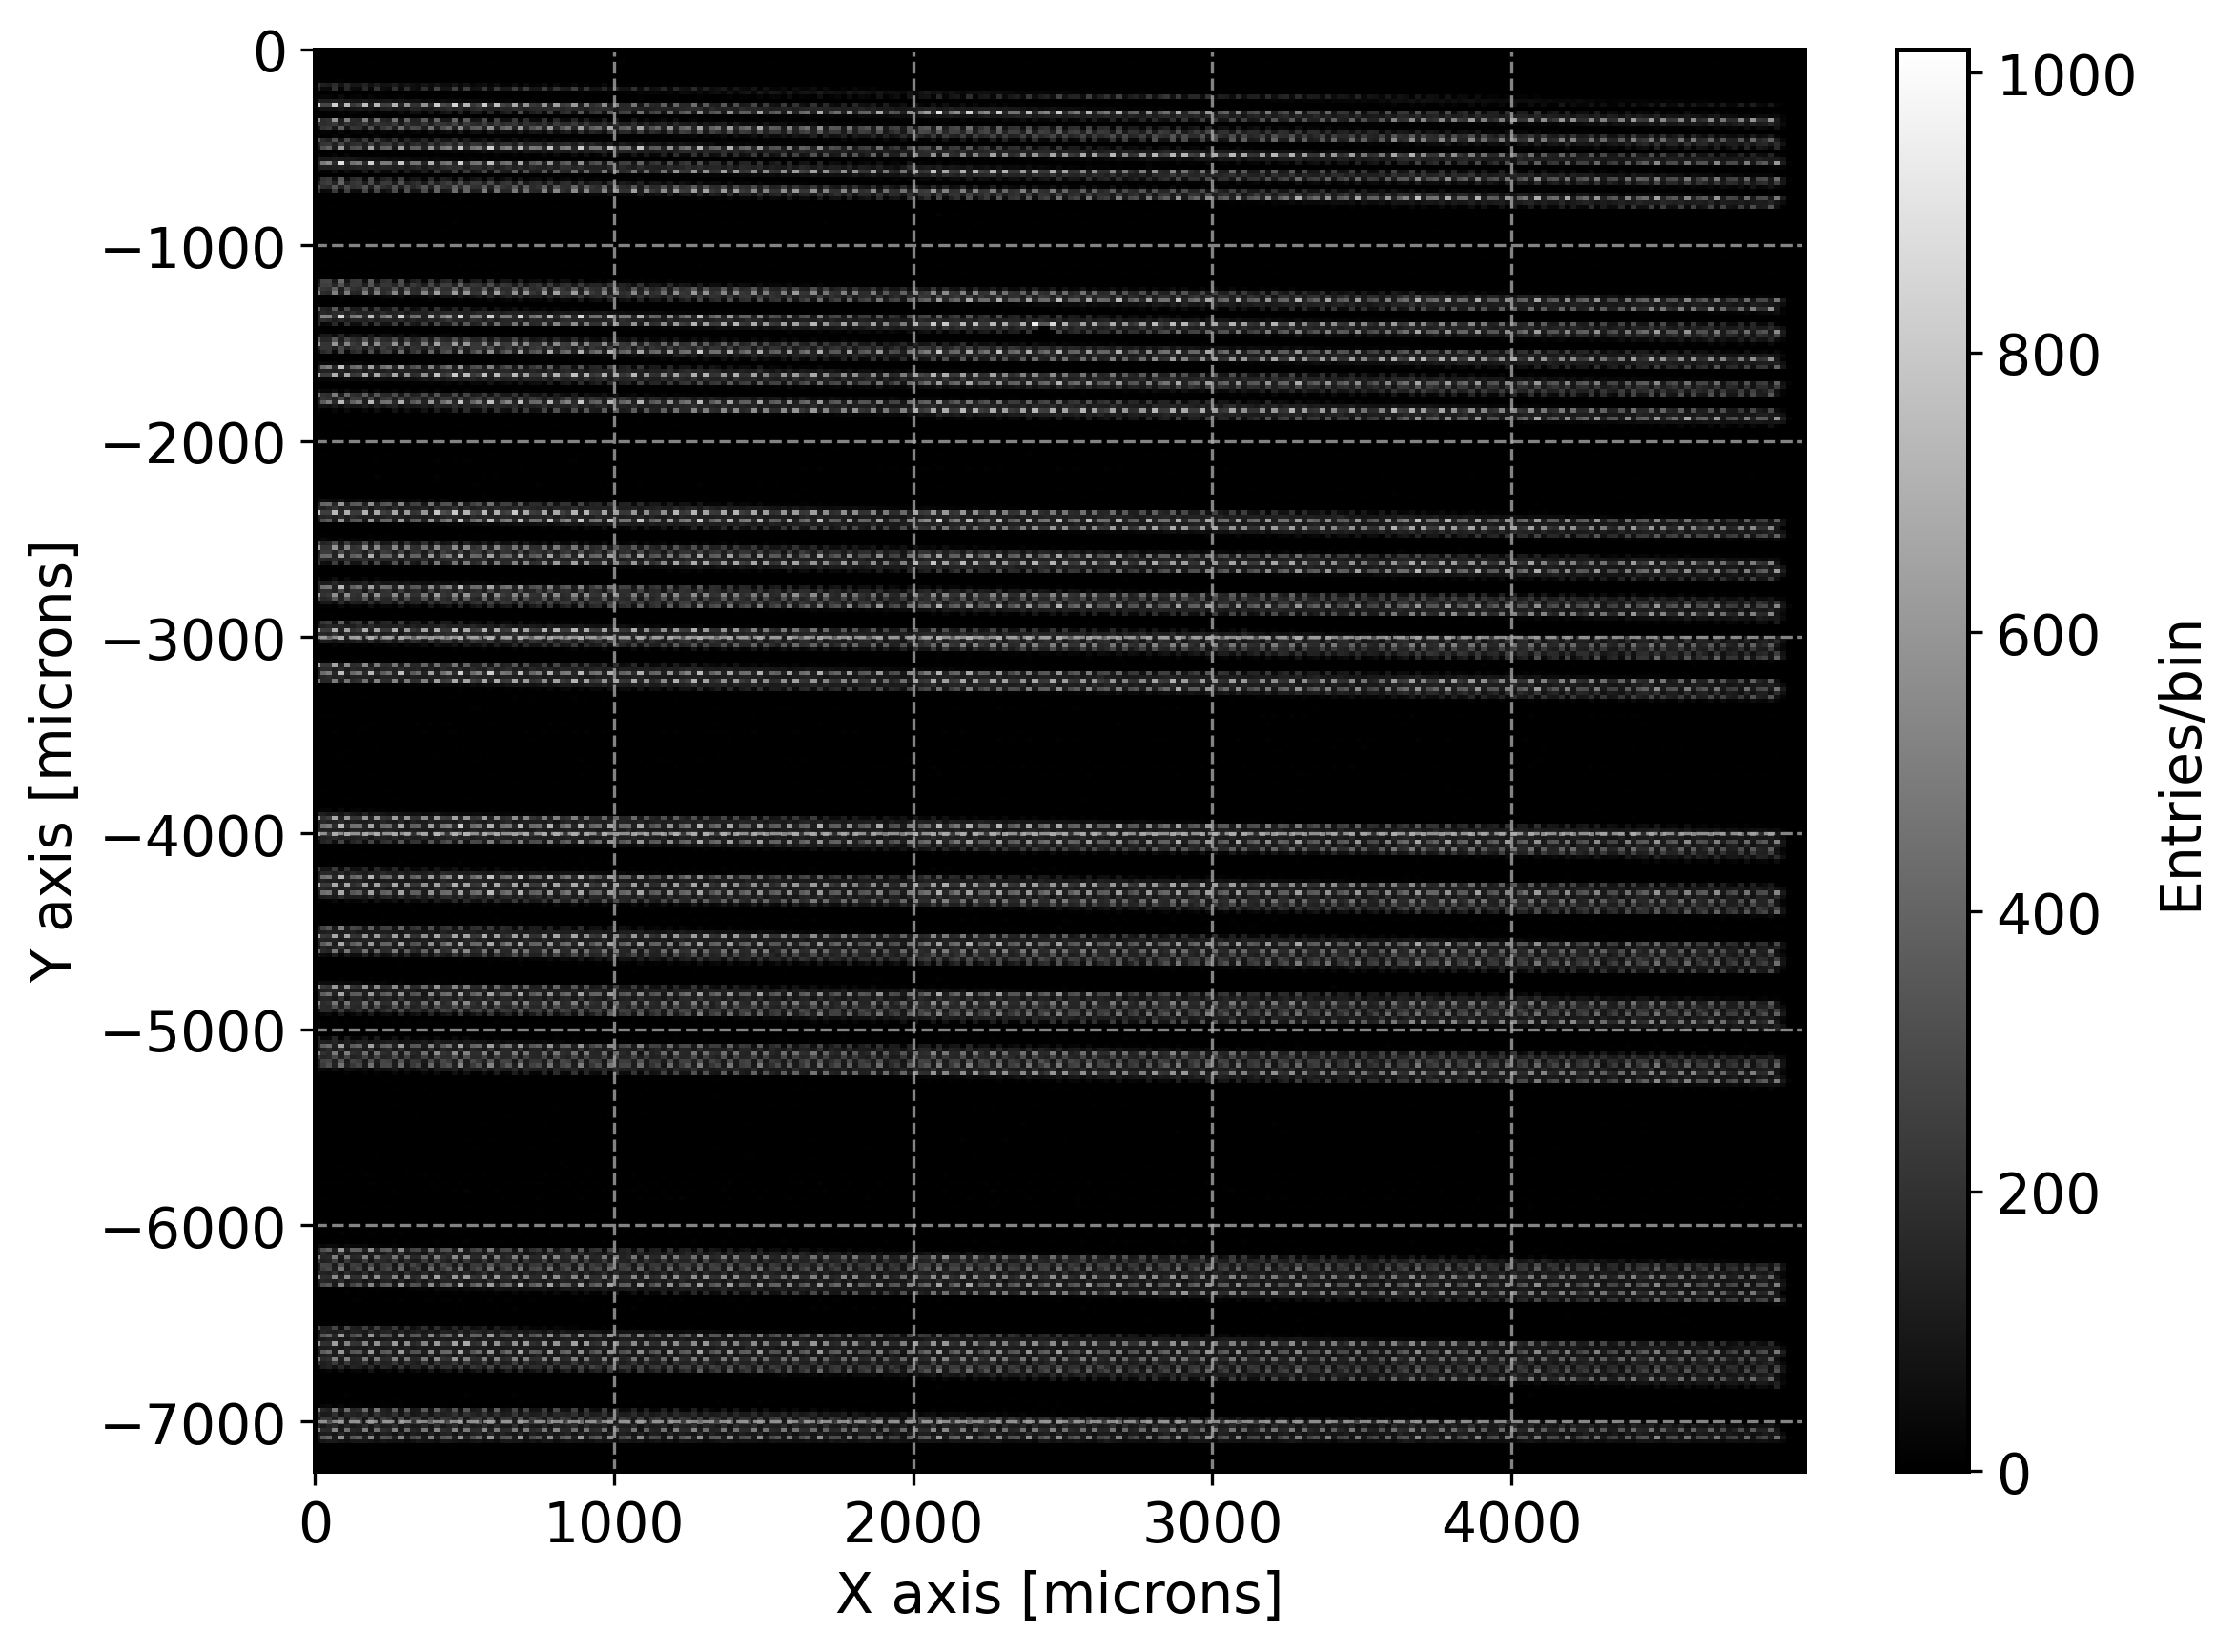
\includegraphics[width=0.59\linewidth]{figures/chapter4/results/slits_hist}
    \caption{The left panel shows an example of Huttner phantom similar to the one employed in the experimental setup. The right panel shows the phantom reconstructed image using the centroid algorithm. It is possible to observe differnent slit sets with various frequencies.}
    \label{fig:huttner}
\end{figure}

Reducing this noise is precisely the major improvement of the final design, which will allow the achievement of very high resolutions in both imaging and spectroscopy. In the current setup, in fact, the total noise is largely dominated by the electronics. However, even in this high-noise regime, the collected data allow us to verify the effectiveness of the developed algorithms and to study how the choice of the method affects the final resolution.

Additionally, these datasets provide a crucial opportunity to validate the Monte Carlo simulations against real data. Accurate simulations are not only important to understand the intrinsic limits of the detector based on its physical properties, but they are also strictly required for the calibration of some of the reconstruction methods.

In this section, the experimental setups used to collect the data for the imaging and spectral resolution estimation are described. Furthermore, dedicated Monte Carlo simulations matching these setups are presented. These simulations are used to calibrate the different reconstruction algorithms and to provide a baseline for comparing the final resolution results.

 
\subsection{Spatial resolution}
To estimate the detector spatial resolution a Huttner phantom similar to the one shown in Fig. \ref{fig:huttner} has been used. The phantom is made of a 50 $\mu$m thick lead slab with multiple sets of slits with different spatial frequencies, ranging from a minimum of 0.5 lp/mm up to a maximum of 10 lp/mm.

\begin{figure}[!b]
    \centering
    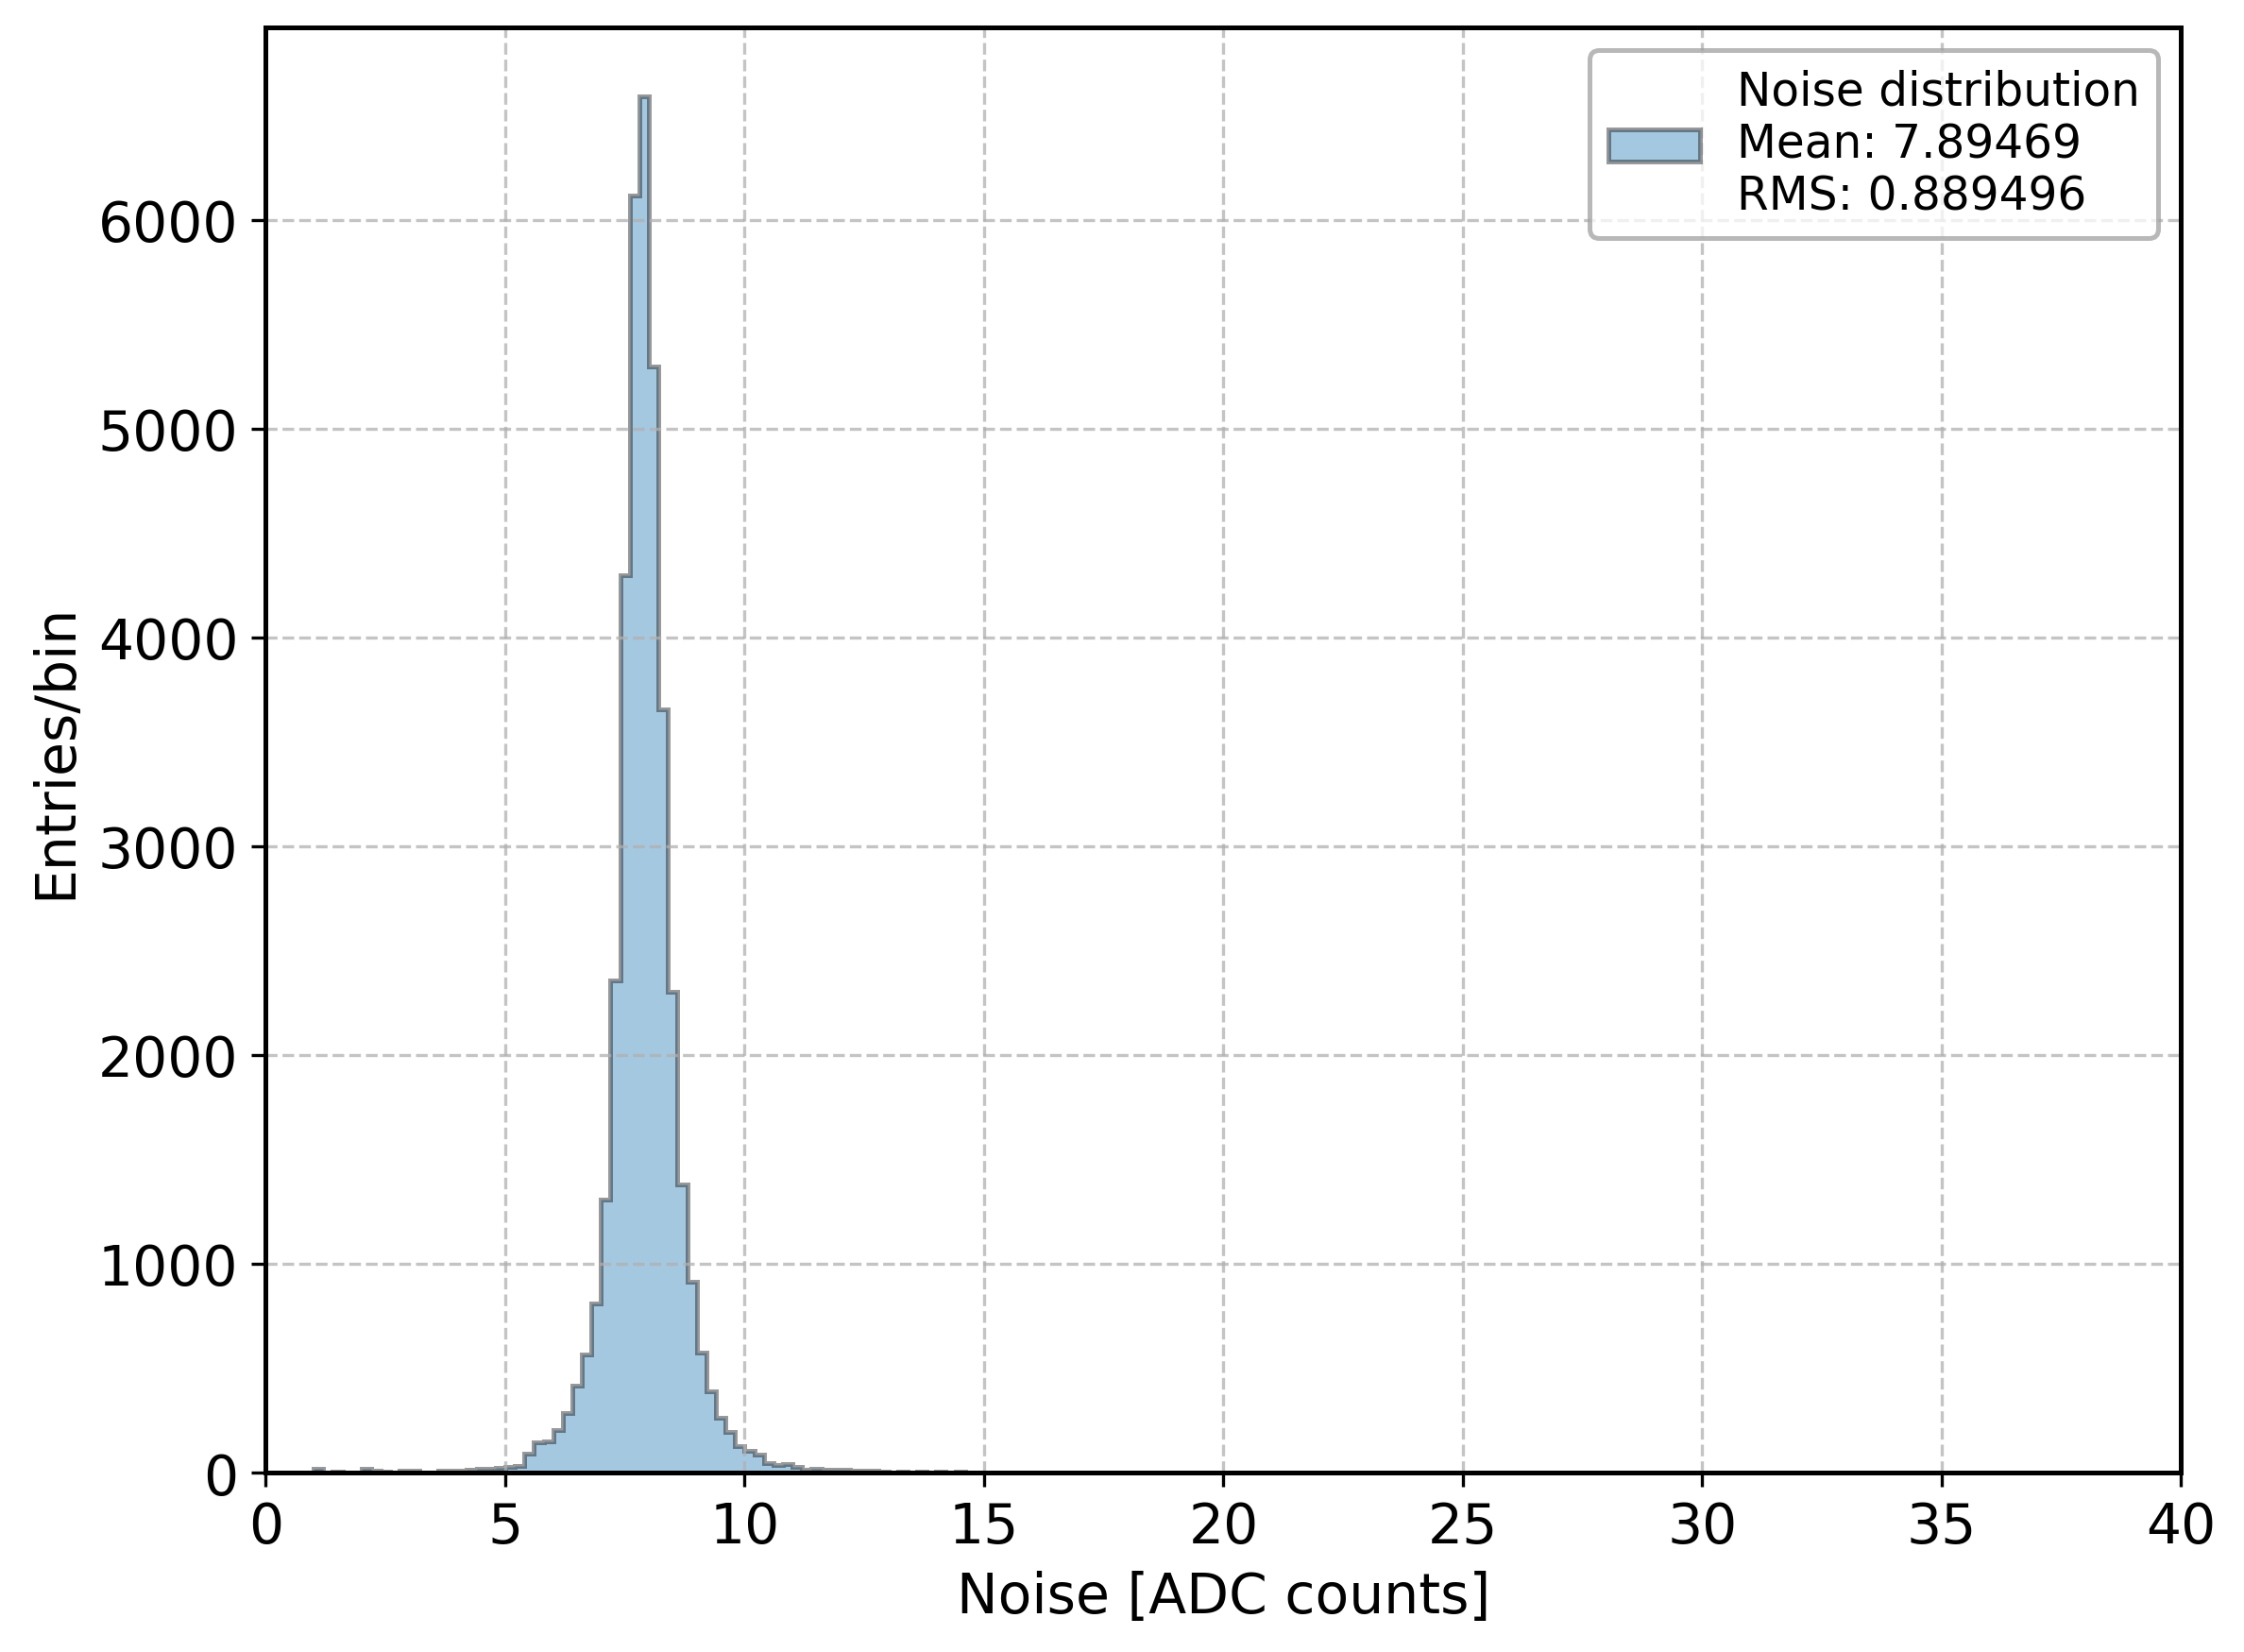
\includegraphics[width=0.49\linewidth]{figures/chapter4/results/noise_hist}
	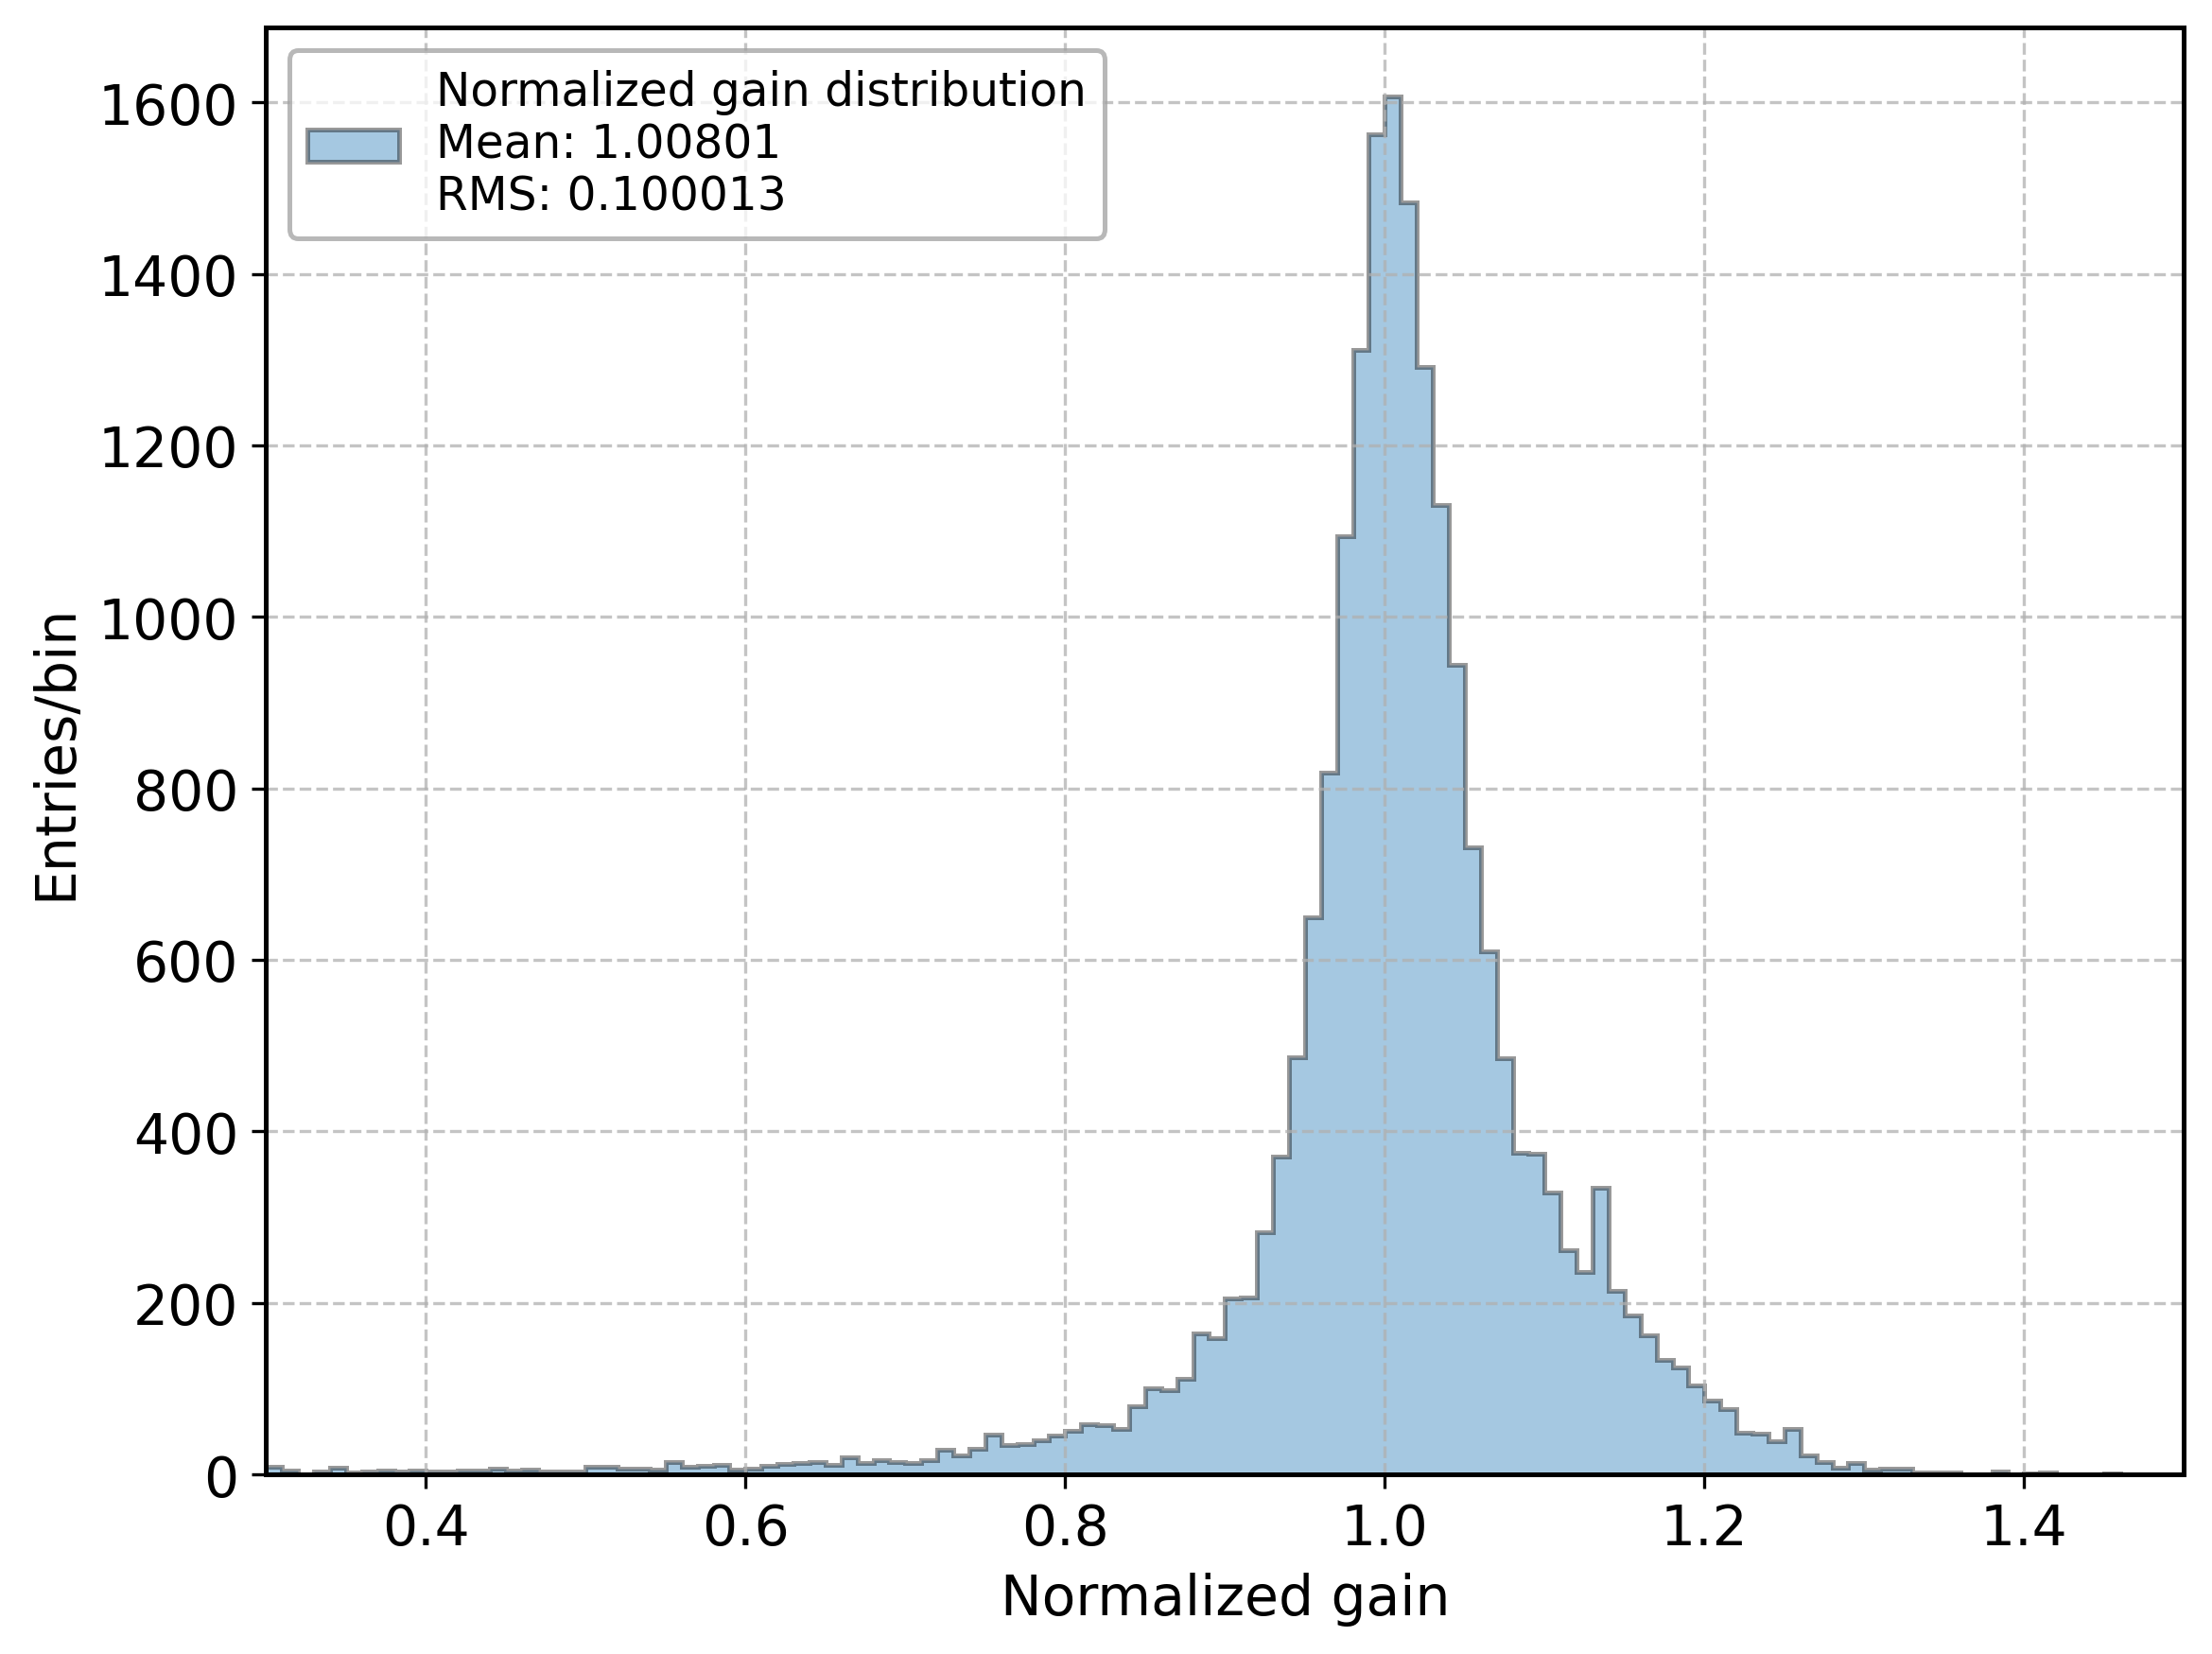
\includegraphics[width=0.49\linewidth]{figures/chapter4/results/equalization_hist}
    \caption{Calibration products obtained from the Huttner phantom laboratory data set. The noise distribution (left panel) has a mean of about 8 ADC counts and a standard deviation of 0.9 ADC counts. The normalized gain has a variation of 10\%.}
    \label{fig:results_cal}
\end{figure}

The phantom portion with the highest frequencies is placed above the detector and it is irradiated with X-rays generated by an X-ray tube which is operated at 10 kV with a gold target \cite{minuti2025}. The X-ray tube is located 1 m from the phantom, in order to have a collimated photon beam. Operating the tube at a voltage of 10 kV with a gold target is not enough to observe fluorescence lines, thus the resulting spectrum is mainly due to Bremsstrahlung emission from accelerated electrons. 

The tested prototype is the one with the silicon sensor, which have pixels with 50 $\mu$m pitch. Given that the expected resolution is smaller than the pixel pitch, the available Hutnner phantom does not have a frequency large enough to be used for a visual estimate of the resolution. The solution is to use the edge of a large slit to calculate the ESF, from which the MTF can then be calculated.

Before the event reconstruction, the detector calibration is performed to estimate the noise level of the pixels. Given that for XPOL-III the pedestal subtraction is performed directly on the chip, the first noise calibration method described in Chap. \ref{sec:calibration} is adopted. Then, the normalized pixel gain is calibrated. The noise and normalized gain distributions are shown in Fig. \ref{fig:results_cal}.

\begin{table}[!t]
\centering
\begin{tabularx}{\textwidth}{X cc}
Reconstruction Algorithm & $f_{10}$ Lab. data [lp/mm] & $f_{10}$ Sim. data [lp/mm]\\
\midrule
Charge barycentering & 47.1 & 53.9 \\
MLE                  & 51.7 & 68.0 \\
Unmodeled $\eta$     & 51.9 & 71.0 \\
Modeled $\eta$       & 51.7 & 67.4 \\
\bottomrule
\end{tabularx}
\caption{Values $f_{10}$ for which $\operatorname{MTF}(f_{10}) = 0.1$ for different reconstruction algorithm calculated for laboratory data and simulated data.}
\label{tab:results_mtf}
\end{table}

\begin{figure}[!b]
    \centering
    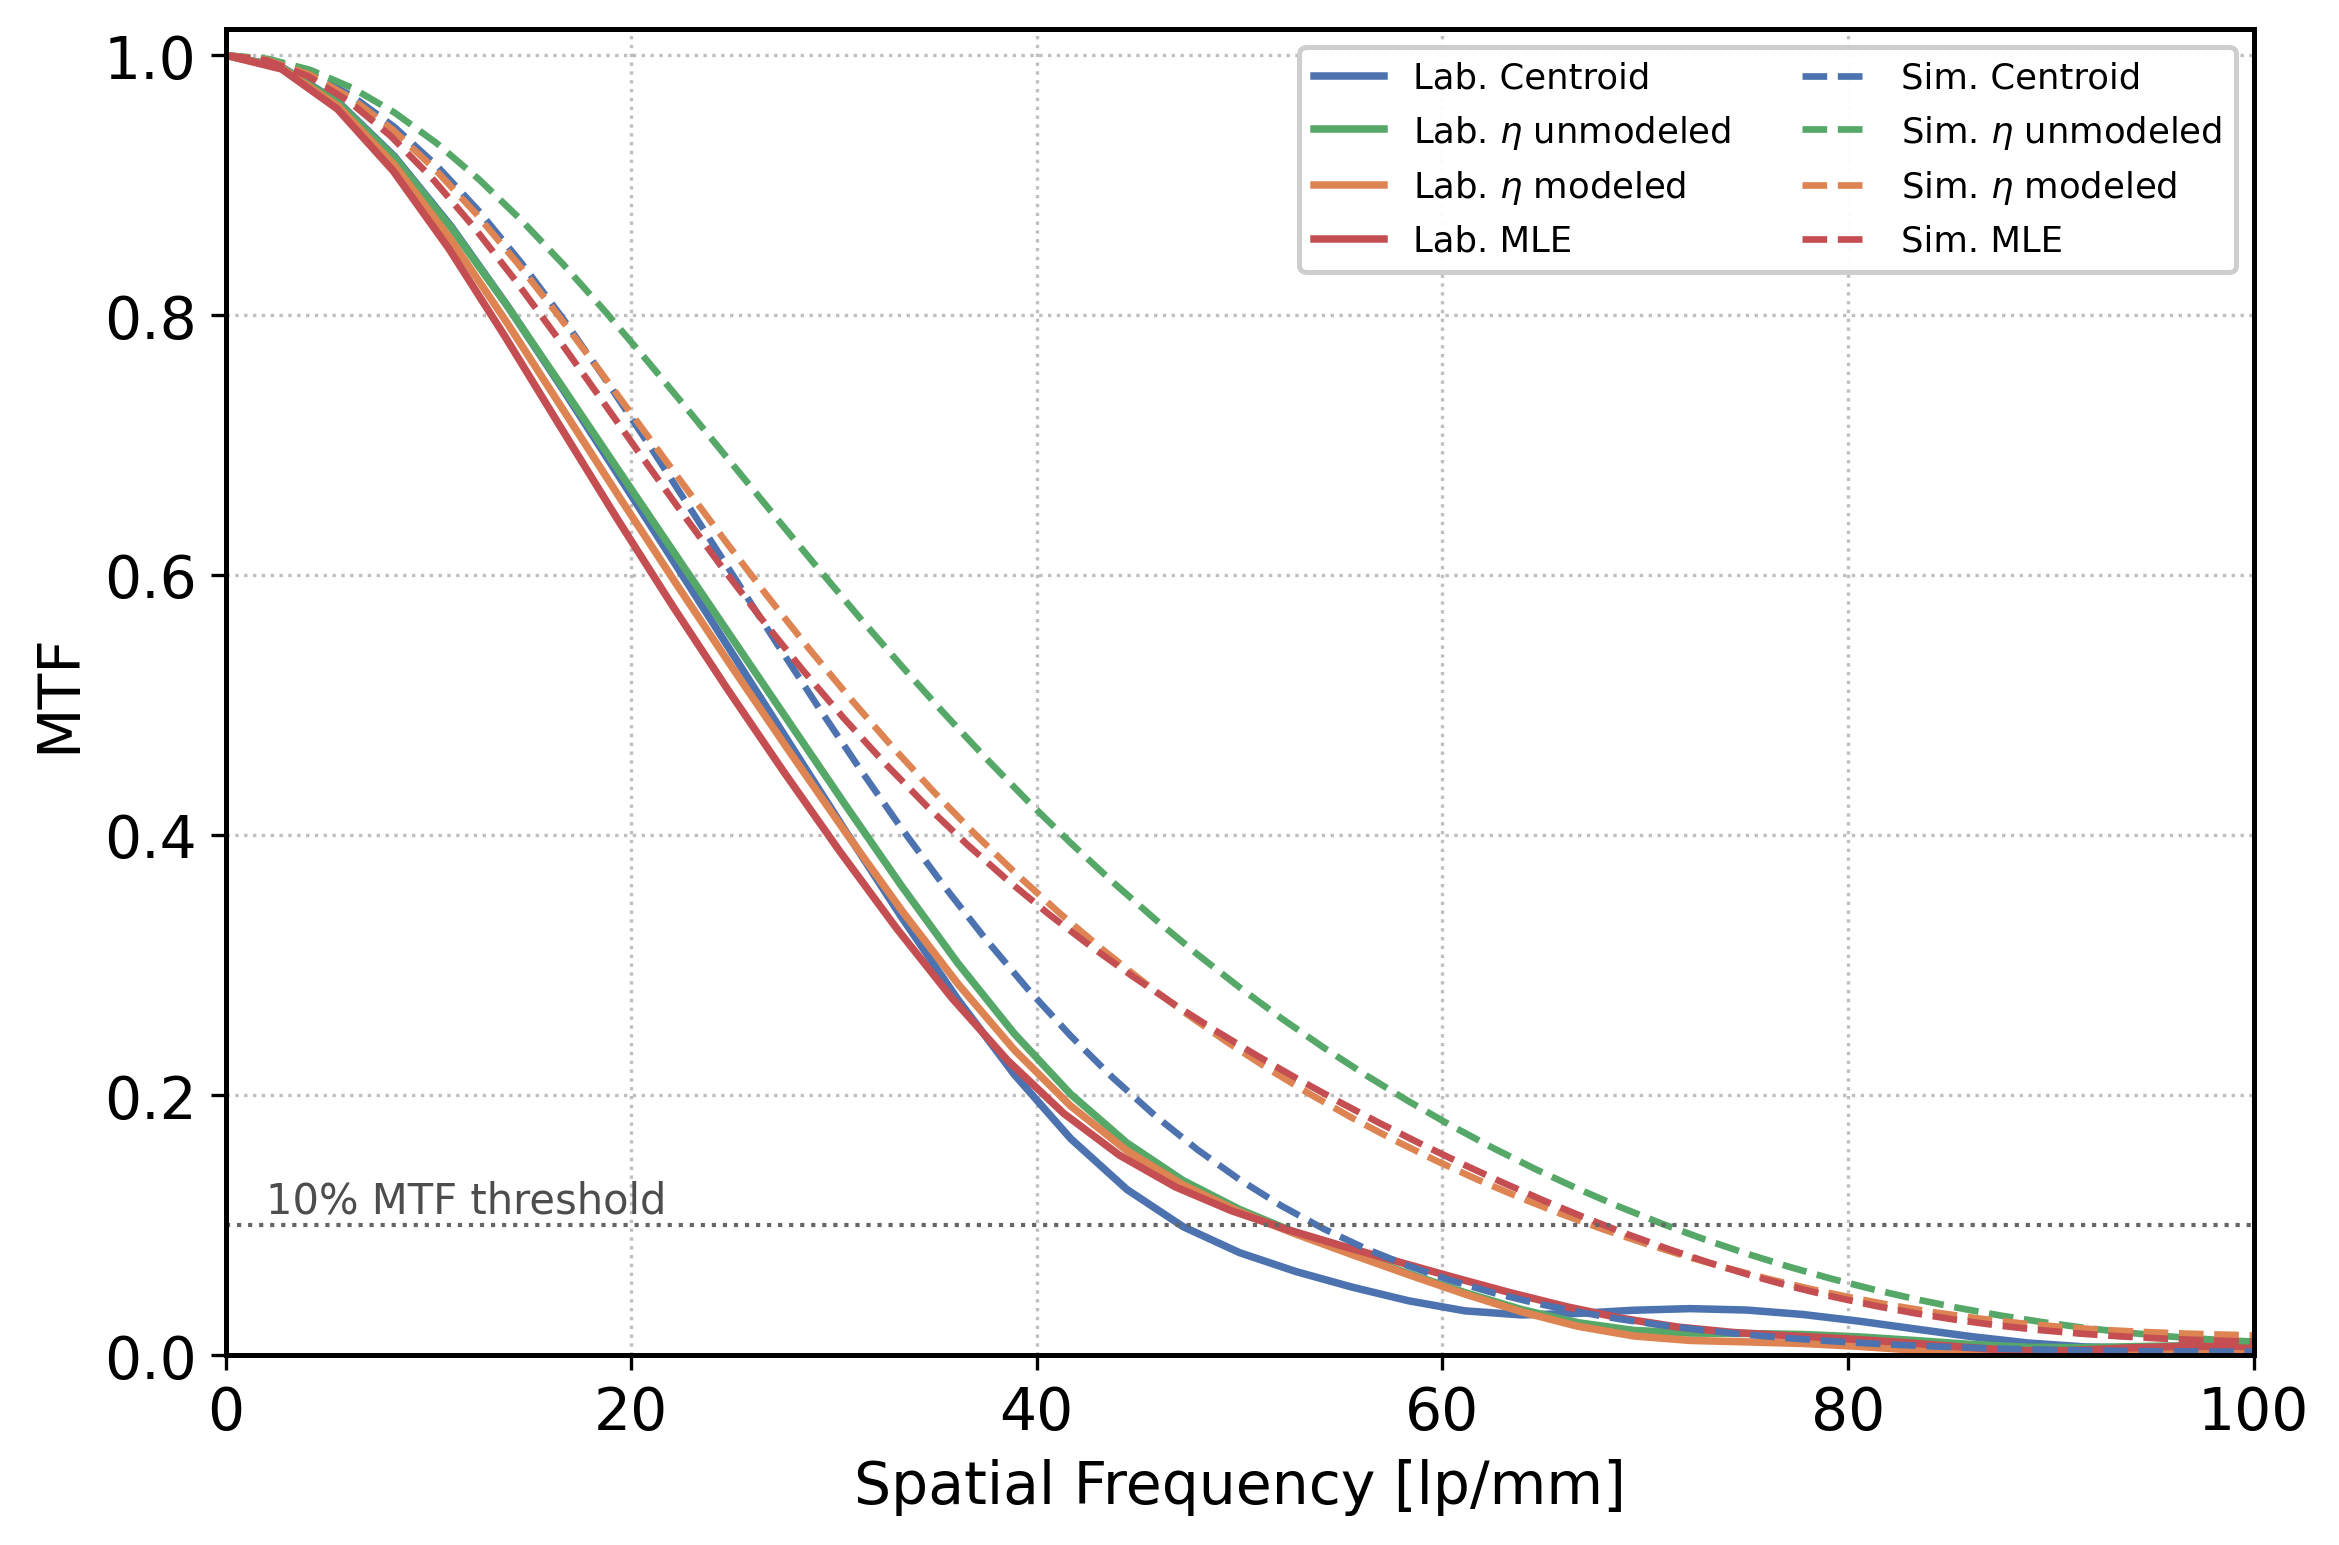
\includegraphics[width=0.7\linewidth]{figures/chapter4/results/slits_mtf}
    \caption{Modulation transfer function obtained with different reconstruction methods for laboratory data and simulated data. Solid lines represent MTF calculated from laboratory data. Dashed lines represent MTF calculated from simulated data}
    \label{fig:results_mtf}
\end{figure}


Once the noise and gain of the detector are characterized, a simulated dataset with matching noise, gain and spectrum shape is generated to calibrate the reconstruction methods. After that, the laboratory data can be analyzed and the event positions can be estimated with the different algorithms. The resulting positions are shown in Fig. \ref{fig:huttner} and it is possible to observe the distribution of the positions along the phantom slits. To estimate the spatial resolution, the method described in Chap. \ref{subsec:mtf} to align and project the reconstructed positions along the axis perpendicular to the slanted slit is used to calculate the MTF.

A new Monte Carlo data set with a slit of the same size of the one analyzed in the laboratory data is simulated to compare the obtained results with those expected from simulations. The data set is generated using the same distribution of noise and normalized gain. After the data set is generated, it is analyzed with the same method used for laboratory data. The MTFs obtained with the different algorithms for laboratory data and simulated data are shown in Fig. \ref{fig:results_mtf} and the values $f_{10}$ for which MTF is 10\% are reported in Tab. \ref{tab:results_mtf}. 

From the analysis of laboratory data, the improvement in the spatial resolution obtained using more complex algorithms than charge barycentering is not as big as expected. Indeed, from Monte Carlo simulations the resolution achieved with the best algorithm, the $\eta$ unmodeled, is about 30\% better than charge barycentering. This behavior can be associated to different factors. An example is the possibility of having defects in the Huttner phantom slit edges. Indeed, the Huttner phantom is designed to have a quick estimate of the resolution and is not ideal to carry on a detailed analysis with the slanted edge. These defects can transmit unwanted photons, thus producing a degraded edge image.

\subsection{Energy resolution}
To estimate the energy resolution, a different experimental setup has been employed. For this purpose it is essential to produce a known spectrum with separated lines. To test the ASIX silicon prototype a gold target has been irradiated by an X-ray tube operated at 25 kV, in order to produce fluorescence lines.

To suppress the Bremsstrahlung continuum spectrum and only detect fluorescence lines, the gold target is tilted with respect to the X-ray tube and only the fluorescence radiation, which is emitted isotropically, reaches the detector. The experimental setup is shown in Fig. \ref{fig:spectral_setup}. With this setup the beam is very small and collimated and it illuminates only an area of about 50 pixels. The observed spectrum shows fluorescence lines produced by $L$-shell transitions. In particular the dominant lines are the $L\alpha$ doublet at about 9.7 keV, the $L\beta$ doublet at 11.5 keV and the $L\gamma$ triplet at 13.4--13.8 keV.

\begin{figure}[htbp]
  \centering
  \begin{tikzpicture}[>=LaTeX, font=\sffamily]

    % Colori
    \definecolor{tubeBody}{RGB}{240, 240, 240}
    \definecolor{goldColor}{RGB}{245, 195, 35}
    \definecolor{detectorColor}{RGB}{235, 235, 235}
    \definecolor{xrayPrimary}{RGB}{210, 40, 40}
    \definecolor{xrayFluo}{RGB}{30, 110, 220}

    % 1. TUBO A RAGGI X ORIZZONTALE (A sinistra)
    \begin{scope}[shift={(-4.2, 0)}]
      % Struttura esterna
      \draw[thick, fill=tubeBody, rounded corners=3pt] (-1.5, -0.6) rectangle (1.5, 0.6);
      % Anodo interno
      \draw[thick, fill=gray!50] (0.8, -0.4) -- (1.1, -0.4) -- (0.7, 0.4) -- (0.4, 0.4) -- cycle;
      % Filamento / Catodo
      \draw[very thick, gray!80] (-1.0, -0.25) -- (-1.0, 0.25);
      \draw[thick, gray!80] (-1.0, 0) -- (-0.4, 0);
      % Finestra di uscita
      \draw[thick, fill=white] (1.5, -0.3) rectangle (1.6, 0.3);
      \node[above, font=\sffamily\small] at (0, 0.65) {X-ray tube};
    \end{scope}

    \coordinate (Source) at (-2.6, 0);

    % 2. TARGET: FOGLIO D'ORO INCLINATO A -45° (Centro in (0,0))
    \coordinate (Target) at (0, 0);

    \begin{scope}[rotate around={-45:(Target)}]
      \draw[thick, fill=goldColor] (-1.2, -0.09) rectangle (1.2, 0.09);
    \end{scope}

    \node[right, font=\sffamily\small, align=left] at (0.8, 0.8) {Au target};
    \draw[->, thick, gray!80] (0.8, 0.6) -- (0.25, 0.25);

    % 3. FASCIO PRIMARIO ORIZZONTALE (Incide al centro della foglia in (0,0))
    \draw[ultra thick, xrayPrimary, ->] (Source) -- (Target) 
      node[midway, above, font=\sffamily\small\bfseries, text=xrayPrimary] {};

    % 4. DETECTOR (Centrato rispetto a (0,0), parallelo al pavimento)
    \coordinate (DetCenter) at (0, -2.5);
    \draw[thick, fill=detectorColor] (-1.3, -2.9) rectangle (1.3, -2.1);
    \node[font=\sffamily\small] at (DetCenter) {Detector};

    % 5. EMISSIONE DI FLUORESCENZA IN RIFLESSIONE (Isotropica)
    % Raggio centrale che va al centro del detector (0, -2.1)
    \draw[thick, xrayFluo, ->] (Target) -- (0, -2.1);
    
    % Raggi laterali verso le estremità del detector
    \draw[thick, xrayFluo, ->] (Target) -- (-0.9, -2.1);
    \draw[thick, xrayFluo, ->] (Target) -- (0.9, -2.1);

    % Frecce tratteggiate esterne (indicatrici dell'emissione isotropica)
    \foreach \angle in {210, 235, 305, 330} {
      \draw[thick, xrayFluo, ->, >=stealth, dashed] (Target) -- (\angle:1.8);
    }

    \node[right, font=\sffamily\small, text=xrayFluo, align=left] at (1.5, -1.2) {Isotropic fluorescence\\radiation};

  \end{tikzpicture}
  \caption{Scheme of the experimental setup for spectral resolution study. The X-ray tube illuminates the Au target which in turn emits fluorescence radiation that irradiates the detector.}
  \label{fig:spectral_setup}
\end{figure}

Before analyzing the data, the detector calibration procedure is performed in order to compensate variations between the pixels. The noise level distribution is approximately a Gaussian with mean around 8 ADC counts and a standard deviation of about 1 ADC counts. The normalized gain is approximately uniform with a standard deviation of 3\%. The obtained calibration products are also used to run a Monte Carlo simulation with the $L\alpha$ and $L\beta$ gold lines and with the same noise and gain distributions of the detector, in order to compare the results between the two datasets.

The energy is then reconstructed using the two methods described in the previous section. When applying the suppression algorithm, different thresholds can be adopted, making it relevant to investigate how the threshold affects the energy resolution. To evaluate the resolution, the $L\alpha$ and $L\beta$ lines are fitted simultaneously using the model described in Eq.~\ref{eq:two_lines_fit}, and the resolution is derived from the FWHM of the $L\alpha$ peak. 

An example of a measured spectrum along with its best-fit curve, as well as the dependence of the energy resolution on the threshold for both experimental and simulated datasets, are shown in Fig.~\ref{fig:spectrum_fit}. While for laboratory data the best energy resolution is achieved at a threshold around 2.5--3.0\,$\sigma$, in the simulations the optimal resolution is obtained with zero threshold. The origin of this discrepancy is not fully understood, but it can likely be attributed to secondary, low-intensity lines present in the experimental gold spectrum that are not modeled in the simulation, as well as pixel-correlated noise sources present in the real setup. Despite this difference, the best energy resolution measured for both datasets, which is 13.5\% (1300 eV) for laboratory data and 12.5\% (1200 eV) for simulated data, does not differ significantly from the expected energy resolution at 9.7 keV of about 11\% (970 eV).

\begin{figure}[!b]
    \centering
    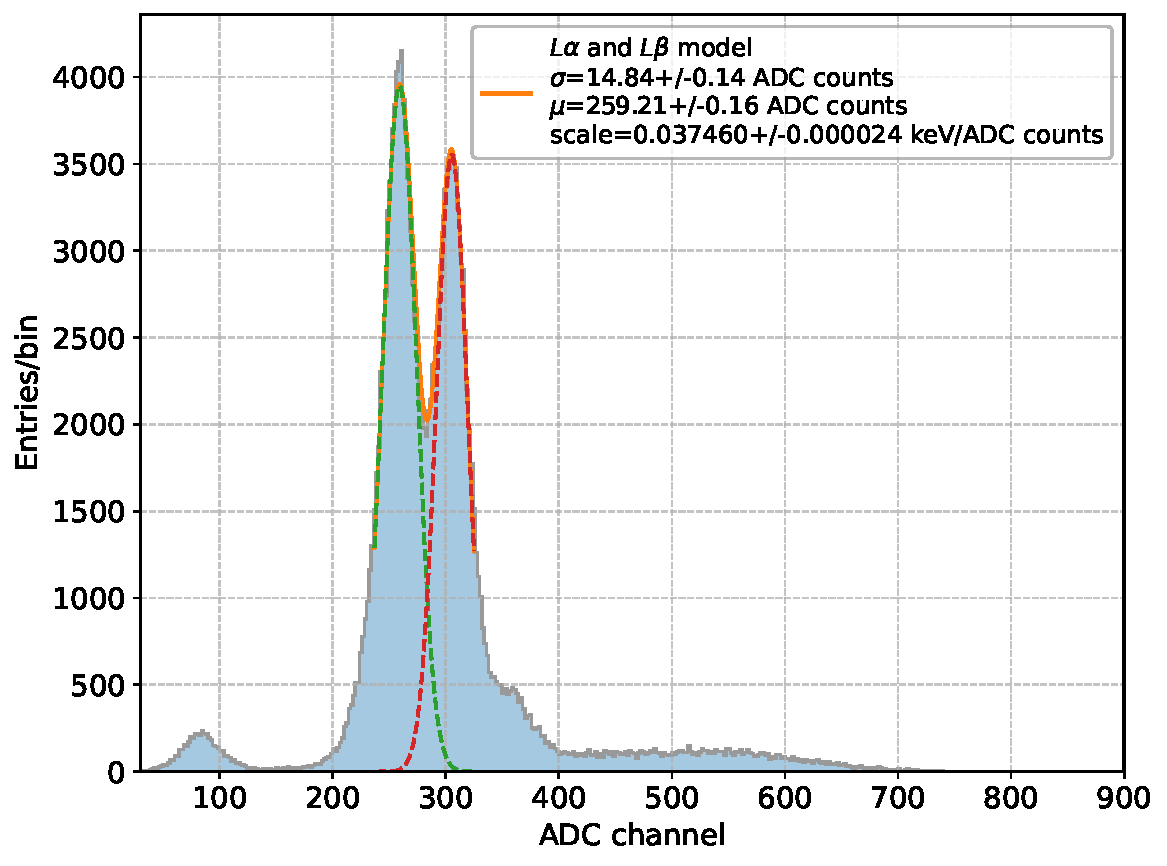
\includegraphics[width=0.49\linewidth]{figures/chapter4/results/spectrum_example}
    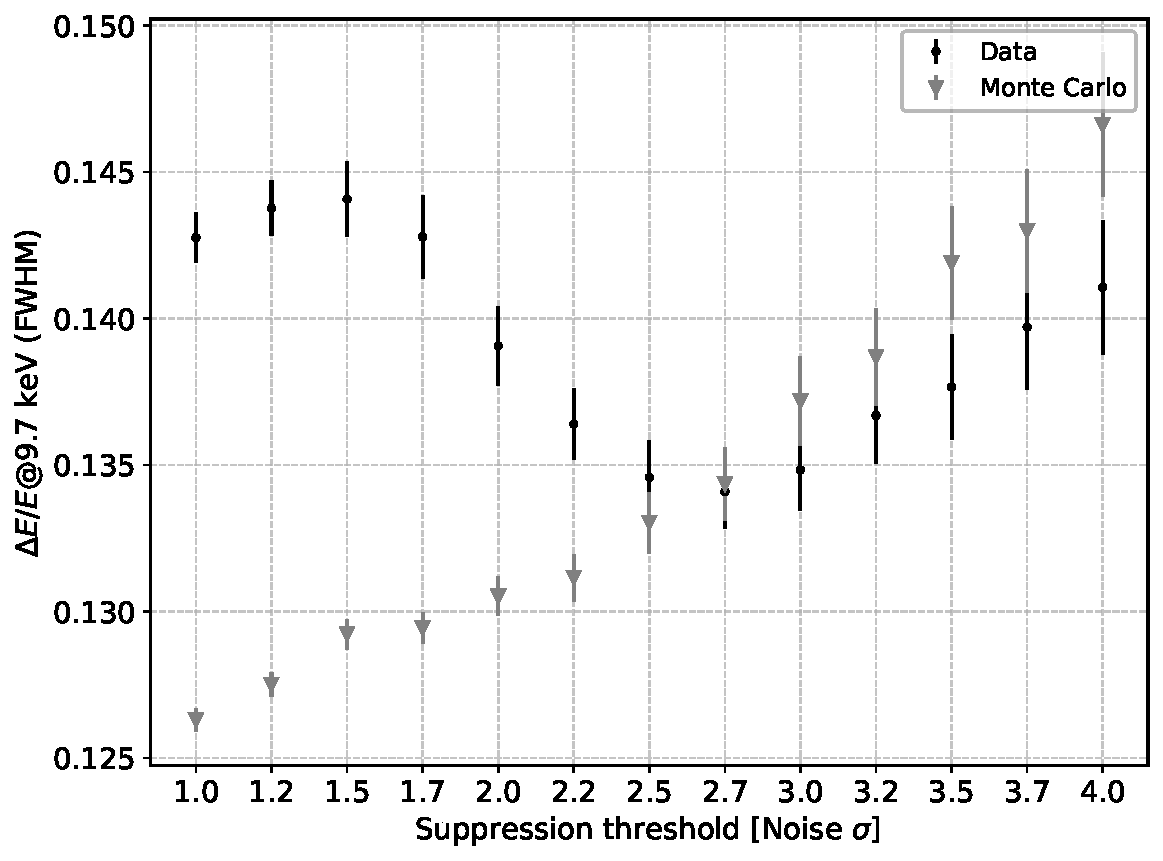
\includegraphics[width=0.49\linewidth]{figures/chapter4/results/zsup_dependence}
    \caption{Example of Au spectrum obtained from an X-ray tube  operated at 25 kV (left panel). The two dominant lines are gold fluorescence lines $L\alpha$ at 9.7 keV and $L\beta$ at 11.5 keV. The spectrum is obtained with a zero-suppression threshold of 2.5$\sigma$ of noise and shows all the events. The dependence of energy resolution on the threshold (right panel) shows that for laboratory data the best resolution is achieved at around 2.5--3.0$\sigma$, while for Monte Carlo simulations it is achieved with lower threshold values. The two dashed lines with the respective error bands show the energy resolution estimate with the MLE algorithm, which is independent from the suppression threshold.}
    \label{fig:spectrum_fit}
\end{figure}

Both laboratory and simulated datasets were also analyzed using the MLE algorithm. For experimental data, the MLE achieves an energy resolution slightly worse than the optimal value obtained with the suppression method. This discrepancy arises from the algorithm's calibration, which relies on Monte Carlo simulations: differences between the simulated and real detector response degrade the reconstruction accuracy. On the other hand, when applied directly to simulated data, the MLE reaches an energy resolution comparable to the best performance achieved by the suppression method. Further measurements are required to determine whether the higher complexity of the MLE algorithm is justified, given that the simpler suppression algorithm achieves the same or even better results on real data.

In conclusion, the current prototype is far from the design goal of 20\,$e^-$ ENC of noise per pixel, which can be achieved only with the ASIC that is currently being designed. At the moment, the single-pixel noise contribution is around 400\,eV. The results obtained with this prototype validate the reconstruction framework and demonstrate the effectiveness of both offline algorithms. Once the final low-noise front-end electronics is coupled to the active sensor, the energy resolution is expected to improve by a factor of 4--5, reaching the targeted $\sim$300\,eV FWHM at 10\,keV and enabling the separation of closely spaced fluorescence lines in applications such as XRD and astrophysical spectroscopy.

\subsection{Cluster size distribution}

\begin{figure}[!b]
\centering
	$\vcenter{\hbox{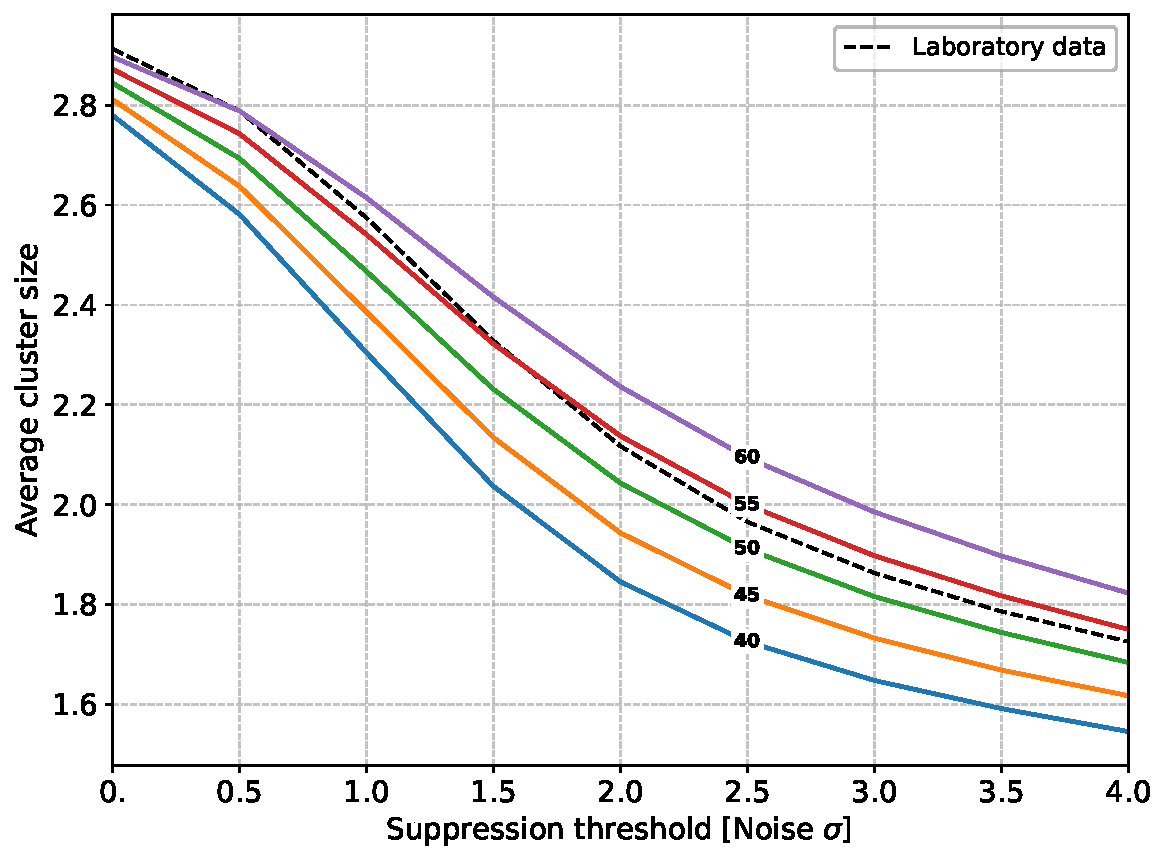
\includegraphics[width=0.55\linewidth]{figures/chapter4/results/cluster_size}}}$\hfill
    $\vcenter{\hbox{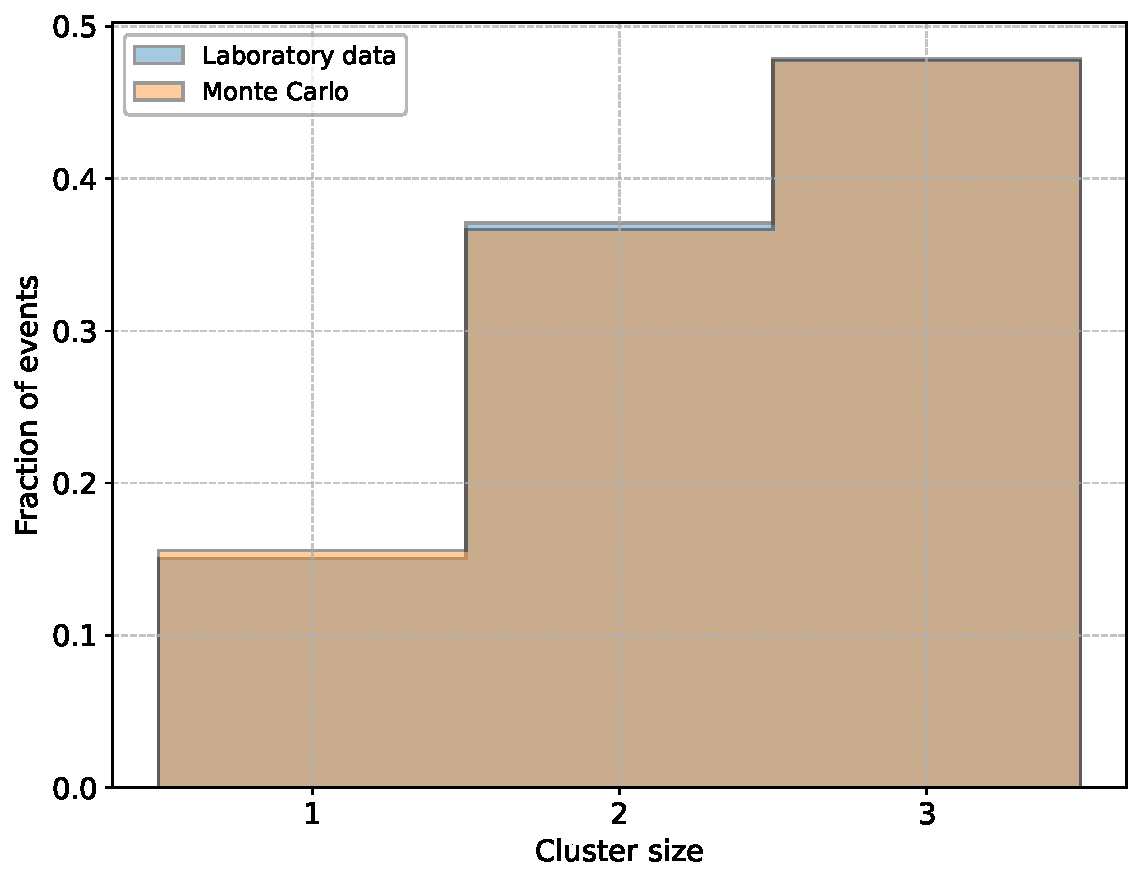
\includegraphics[width=0.45\linewidth]{figures/chapter4/results/cluster_size_hist}}}$
    	\caption{Average cluster size as a function of the zero-suppression threshold for laboratory data and Monte Carlo simulations generated with different diffusion coefficients ranging from 40 to 60 $\mu$m~cm$^{-0.5}$ (left panel). The experimental data points are best matched by the simulation with 55~$\mu$m~cm$^{-0.5}$. Normalized cluster size distribution for laboratory data compared to the Monte Carlo simulation with a diffusion coefficient of 55~$\mu$m~cm$^{-0.5}$, obtained with a zero-suppression threshold of 1.5\,$\sigma$ (right panel).}
\label{fig:cluster_size}
\end{figure}

In addition to comparing the spatial and energy resolutions between laboratory data and Monte Carlo simulations, another relevant quantity that can be evaluated is the cluster size. This metric depends primarily on the charge diffusion geometry and the pixel pitch. While the pixel pitch is precisely known, charge diffusion is harder to estimate accurately due to uncertainties in the diffusion coefficient. In fact, various physical effects, such as local electric field variations, doping non-uniformities, and temperature fluctuations, can introduce a significant uncertainty on its nominal value. Furthermore, pixel crosstalk acts as an additional charge-sharing mechanism, effectively spreading charge across adjacent pixels as if the diffusion coefficient were larger.

For this reason, the effective diffusion coefficient used in the Monte Carlo simulations is tuned by matching the laboratory data. Specifically, events are reconstructed with different zero-suppression thresholds, following the same procedure adopted for the energy reconstruction, to evaluate the average cluster size distribution. Multiple datasets matching the experimental source spectrum, noise, and gain are then simulated for different diffusion coefficients.

The comparison between experimental and simulated data is shown in Fig.~\ref{fig:cluster_size}. For the gold spectrum dataset used to evaluate the energy resolution, the diffusion coefficient that best describes the experimental data is found to be around $55\,\mu\text{m}\,\text{cm}^{-0.5}$. This agreement is confirmed by comparing the cluster size distributions, particularly at a threshold of $1.5\,\sigma$.

\section{Conclusions}
In summary, the characterization of the current ASIX prototypes has successfully validated both the proposed architecture and its dedicated simulation and analysis framework. By combining experimental measurements, using line pair phantoms for spatial resolution and fluorescence targets for spectroscopy, with Monte Carlo simulations, a complete data processing pipeline has been established and tested. This framework covers the entire analysis workflow: it starts from the fundamental calibration of detector non-uniformities, such as noise levels, baseline offsets, and normalized gain, and integrates these products into the event reconstruction process to improve the estimate of the photon energy and its sub-pixel incidence position.

Although the experimental spatial and energy resolutions are currently constrained by the high electronic noise of the XPOL-III readout chip, the implementation of advanced reconstruction algorithms confirms the validity of the underlying physical models. In particular, both the maximum likelihood estimator and the $\eta$ algorithms have demonstrated their superiority over simple charge barycentering, proving that exploiting the charge sharing geometry is the key to achieving sub-pixel spatial resolution. Furthermore, the agreement found between experimental data and simulations, such as in the matching of the cluster size distributions, proves the reliability of the current simulation software for these preliminary studies. However, since the current Monte Carlo framework is based on a simplified physical model, it will need to be upgraded by integrating a full Geant4 simulation to accurately account for all the relevant physical processes.

The integration of a new low-noise XPOL ASIC, with a target of less than $20\text{ e}^-$ ENC per pixel and the seven-pixel parallel readout logic, will finally overcome the current hardware limitations. In preparation for this upgrade, the analysis framework discussed in this work provides a validated environment, ready to be employed for the characterization of the final detector in the next development phases.
